\usepackage[english]{babel} % Sets the document language to English
\usepackage{listings} % For including source code listings
\usepackage{hyperref} % For creating hyperlinks within the document
\usepackage[font=small, labelfont=bf]{caption} % Customizes captions for figures and tables
\usepackage{multicol} % Allows multicolumn layout
\usepackage[ruled, vlined, algo2e]{algorithm2e} % Typesets algorithms
\usepackage[toc, page]{appendix} % Adds appendices to the document
\usepackage{float} % Improves the interface for defining floating objects
\usepackage{amsfonts} % Provides additional fonts, especially mathematical symbols
\usepackage{algorithm} % Float environment for algorithms
\usepackage{algorithmic} % Typesets algorithms
\usepackage{amssymb} % Provides various mathematical symbols
\usepackage{derivative} % For typesetting derivatives
\usepackage[framemethod=tikz]{mdframed} % Creates framed boxes with shaded backgrounds
\usepackage{tikz} % Package for creating diagrams and drawings
\usetikzlibrary{shapes, arrows.meta, positioning} % Importing TikZ libraries for additional functionalities.
\usepackage{amsmath} % Enhanced math features
\usepackage{graphicx} % Loading the package for including graphics
\usepackage{amsmath} % Additional math features
\usepackage{mathtools} % Enhances mathematical typesetting
\usepackage[makeroom]{cancel} % Adds a cancellation bar in math mode
\usepackage{subcaption} % Provides support for subfigures and subcaptions
\usepackage{enumitem} % Customizes lists
\usepackage{bbold} % Provides the identity matrix symbol
\usepackage{multirow} % Allows table cells to span multiple rows

\graphicspath{images} % Sets the path for graphics files
\setcounter{secnumdepth}{5} % Sets the depth for section numbering

\lstset{ 
  frame=tb, % Draws a frame at the top and bottom of code blocks
  tabsize=4, % Sets tab space width
  showstringspaces=false, % Does not mark spaces in strings
  numbers=none, % Does not display line numbers
  commentstyle=\color{green}, % Sets the comment color
  keywordstyle=\color{red}, % Sets the keyword color
  stringstyle=\color{blue}, % Sets the string color
  breaklines=true, postbreak=\mbox{\textcolor{green}{$\hookrightarrow$}\space} % Enables line wrapping with a symbol at the end
}

\newcommand{\defi}[1]{\begin{mdframed} [nobreak=true,hidealllines=false,linecolor=blue!40,linewidth=2pt,backgroundcolor=blue!5,]{#1} \end{mdframed}}
% Defines a command for framed definitions with a blue background

\newcommand{\defib}[2]{\begin{mdframed} [hidealllines=false,linecolor=blue!40,linewidth=2pt,backgroundcolor=blue!5,] \begin{center} \textbf{{#1}} \end{center} \vspace{2mm} {#2} \end{mdframed}}
% Defines a command for framed definitions with a blue background and a title

\newcommand{\theo}[1]{\begin{mdframed} [hidealllines=false,linecolor=yellow!40,linewidth=2pt,backgroundcolor=yellow!5,]{#1} \end{mdframed}}
% Defines a command for framed theorems with a yellow background

\newcommand{\sumup}[1]{\begin{mdframed} [hidealllines=false,linecolor=red!40,linewidth=2pt,backgroundcolor=red!5,]{#1} \end{mdframed}}
% Defines a command for framed summaries with a red background

\newcommand{\tab}[1][0.5cm]{\hspace*{#1}} % Defines a command for adding horizontal space

\title{\Huge \textbf{Machine Learning\\} \Large{Andrea Passerini\\a.y. 2022/2023}}

\author{Stefano Genetti\\Vittoria Ossanna\\Giovanni Valer (\LaTeX\ revision)}

\begin{document}
\maketitle

\newpage
\textit{These notes are for the course "Machine Learning" held by professor Andrea Passerini. These notes do not directly cover the laboratory part; still, while discussing the theory many concepts applicable to the laboratory part might be covered. \\
We tried to include most of the materials used during the lectures or given as reference. Our aim was to create notes that allow to get a clear overview of all the topics and to arrange them in a structured manner, while also being fairly exhaustive.\\
We tried our best to avoid mistakes while compiling these notes. That being said, a very broad range of topics was to be covered, hence we do not take responsibility for any mistake or imperfection that might be present; still, it would be much appreciated if you reported any of those to us so that we can fix the notes accordingly.\\
In this \href{https://github.com/StefanoGenettiUniTN/MachineLearning_Passerini.git}{Github repository} you can find the \LaTeX source code, you are free to clone the project and modify it by yourself or just create an issue to include topics and corrections.\\
We hope that this document will help in the study of this beautiful and exciting subject.}
\newline

\textit{If you consider this material valuable for you in order to be prepared for the exam, consider offering us a coffee (-:}\\
Paypal: vittossanna@gmail.com
\newline

\textit{XOXO - the authors}

\newpage

\tableofcontents


    \chapter{Introduction}
\label{cha:intro}

\textit{A computer program is said to \textbf{learn} from experience E with respect
to some class of tasks T and performance measure P, if its performance at task
in T, as measured by P, improves with experience E.}\\

Machine learning is the study of computer algorithms that improve automatically through
experience. The peculiarity of machine learning algorithms is their ability to
learn without being explicitly programmed. Due to these characteristics, ML is
considered a component of the wider artificial intelligence field. The environments
of machine learning techniques application are never ending. Nowadays hot topics
include speech recognition, optical character recognition, computer vision, autonomous
driving, game playing, recommender systems (e.g. Amazon's "suggested for you" sections)
and so on.

\begin{figure}
	\centering
	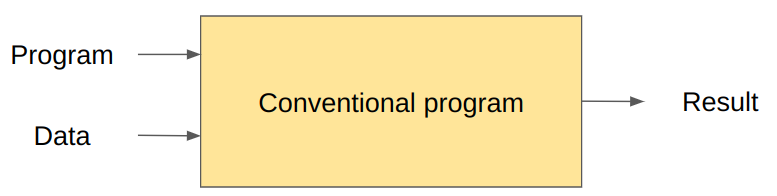
\includegraphics[width=0.8\textwidth]{
		images/01_Introduction_conventionalProgram.png
	}
	\caption{Conventional programming.}
	\label{fig:conventionalProgramming}
\end{figure}

\begin{figure}
	\centering
	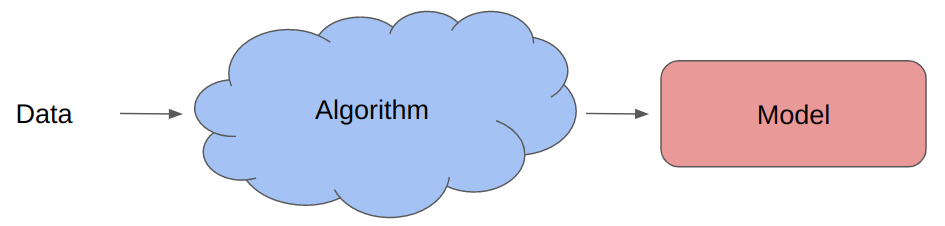
\includegraphics[width=0.8\textwidth]{
		images/01_Introduction_machineLearning.png
	}
	\caption{ML allows computers to \textbf{acquire knowledge}. Knowledge acquired
	is represented by a \textbf{model}. The model is used for \textbf{future} data.}
	\label{fig:mlvsconventionalProgramming}
\end{figure}

\subsubsection*{Components of a well-posted learning problem}
A problem solvable through machine learning techniques relies on three well
defined entities:
\begin{itemize}
	\item the \textbf{task} that we are trying to solve (e.g. recognizing
		handwritten characters),

	\item a \textbf{performance measure} with which we will evaluate the
		performance of the algorithm (e.g. miss-classified items, scoring system...),

	\item the \textbf{training experience} on which the system relies on to learn
		(e.g. data with annotated solutions, labelled handwritten characters).
\end{itemize}

\section{Design of a machine learning system}
A proper design of a machine learning system follows six steps:
\begin{enumerate}
	\item formalize the learning task

	\item collect data

	\item extract features

	\item choose the class of learning models

	\item train the model

	\item evaluate the model
\end{enumerate}

\subsubsection*{Formalize the learning task}
This is a overall definition of the goal we are trying to achieve. This could also
be composed by a chain of separate tasks.\\ Along the definition of the aim, it
is required to define an appropriate performance measure for evaluating the
system.\\ With this first process, we get a formal definition of the problem.
\newline
\textbf{Example:} recognizing handwritten characters from images.

\subsubsection*{Collect data}
A machine learning system requires data, collected in machine readable format, on
which the algorithm will rely for training. This is a delicate and difficult
process because could imply manual intervention for labelling data.\\ Not every
machine learning technique requires annotation of data (semi-supervised and unsupervised
learning).

\subsubsection*{Extract features}
The process of feature extraction consists in representing data in a way in
which a computer can work with, this implies codifying data into other representative
data. Prior knowledge is often needed in order to extract significant features. The
number of features chosen has a relevant impact on the performances: too many
features can require a number of training data much greater, too few could miss relevant
information and decrease the performance. Moreover, by taking into account too many
features, there is the risk of including noisy features which can make the
learning problem harder.

\subsubsection*{Choose the class of learning models}
The choice of the model can heavily impact performance, a simple model classifier
could be insufficient to complete the task while a complex model could lead to \textit{overfitting}.
% \defi{\textbf{Overfitting} \label{def:overfitting}\\ Overfitting is a modeling error that occurs when a function is too closely aligned to a limited set of data points. This happens when in training we achieve top performance while with validation sets they get lower: this could mean that the training took into account also noise among the training data.}
\defi{\textbf{Overfitting}\label{def:overfitting}\\ Overfitting is a modeling error that occurs when a function is too closely aligned to a limited set of data points. This happens when in training we achieve top performance while with validation sets they get lower: this could mean that the training took into account also noise among the training data.}

\subsubsection*{Train the model}
Training a model implies searching through the space of the possible models given
a model class while performance of the model is measured. A trained model should
be able to \textbf{generalize} (perform well on unseen data) and avoid overfitting
\ref{def:overfitting}. Several techniques can be exploited to improve
generalization.

\subsubsection*{Evaluate the model}
The evaluation of the model is based on data which the algorithm has never seen
before. This process identifies weaknesses and give hints on how to improve the model.
Appropriate statistical test need to be carried on to verify significance of the
observed results.

\section{Learning settings}

\subsection{Types of learning methods}
\begin{figure}
	\centering
	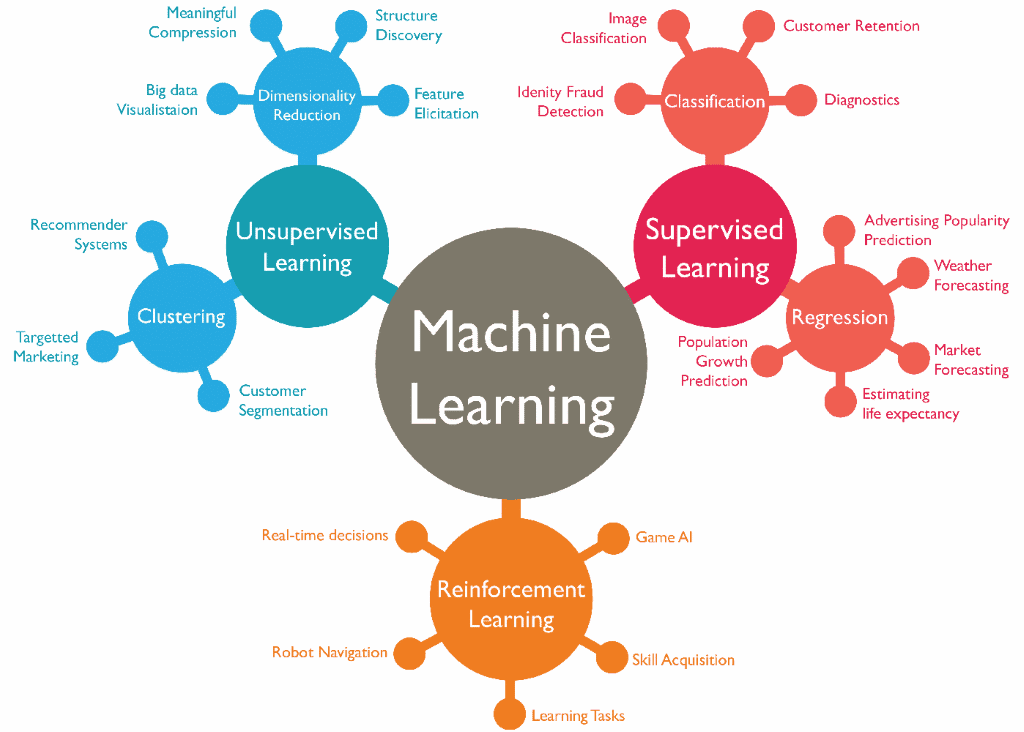
\includegraphics[width=0.8\textwidth]{
		images/01_Introduction_machineLearningAlgorithms.png
	}
	\caption{Main types of learning methods}
	\label{learning_methods_fig}
\end{figure}

Before starting to build a model, it is necessary to choose a type of learning.
Often different data or goals require different learning settings.

\defi{\textbf{Supervised learning \label{def:supervised}\\} The learner is provided with a set of input and output pairs (labelled data) $(x_{i}, y_{i}) \in \mathcal{X}\times \mathcal{Y}$.\\ The learned model $f : \mathcal{X}\rightarrow \mathcal{Y}$ should map input samples into the proper output. A domain expert is often required in order to get labelled inputs. }

\defi{\textbf{Unsupervised learning \label{def:unsupervised}\\} The learner is provided with a set of input but no annotation $(x_{i})\in \mathcal{X}$.\\ The learner models training example, e.g. by grouping them into clusters according to their similarity. These algorithms discover hidden patterns or data groupings without the need for human intervention. }

\defi{\textbf{Semi-Supervised learning \label{def:semi-supervised}\\} The learner is provided with a set of input and output pairs (labelled data) $(x_{i}, y_{i}) \in \mathcal{X}\times \mathcal{Y}$ and a typical much bigger set of unlabelled data $(x_{i})\in \mathcal{X}$.\\ The learned model $f : \mathcal{X}\rightarrow \mathcal{Y}$ should map input samples into the proper output like in supervised learning while unlabelled data can be exploited to improve performances (e.g. improve boundaries). }

\defi{\textbf{Reinforcement learning \label{def:reinforcement}\\} The learner is provided with a set of possible states $\mathcal{S}$ and for each of them a set of possible action $\mathcal{A}$ is available in order to move through the next state. Performing an action $a$ from a state $s$ provides an immediate reward $r(s, a)$ that can be either immediate or delayed.\\ The goal is learning a policy that allows the algorithm to choose between states maximizing the overall reward. Often the model needs to face exploitation (performing moves that are known to be rewarding) and exploration (perform new moves) to avoid getting stuck in a local minimum. }

\subsection{Types of supervised learning tasks}
Before starting to build a model, it is necessary to understand the goal. This
implies understand what kind of classification we are trying to get once the
problem is formalized.

\defi{\textbf{Binary classification} \label{def:binary_classification}\\ The binary classification problem sets its goal into separate samples into two subset (often defined as positive and negative). }

\defi{\textbf{Multiclass classification} \label{def:multiclass_classification}\\ The multiclass classification assigns a sample to a class chosen between $n>2$ different classes. \begin{equation}f: \mathbb{R}^{d}\rightarrow \{1,2,\hdots, n\}\end{equation}}

\defi{\textbf{Multilabel classification} \label{def:multilabel_classification}\\ The multilabel classification assigns a sample to a subset of possible classes (not a unique assignment). E.g. predict the topics of a text. }

\defi{\textbf{Regression} \label{def:regression}\\ This type of problems require to assign a real value to a sample. \begin{equation}f: \mathbb{R}^{d}\rightarrow \mathbb{R}\end{equation}}

\defi{\textbf{Ordinal regression or ranking} \label{def:ranking}\\ A ranking problem sets its goal into defining an order to samples according to their relevance/quality/importance. }

\subsection{Types of unsupervised learning tasks}

\defi{\textbf{Dimensionality reduction} \label{def:dimension_reduction}\\ In dimensionality reduction tasks we are trying to reduce the dimension of the data maintaining as much information as possible. }

\defi{\textbf{Clustering} \label{def:clustering}\\ For clustering we mean divide data into homologous groups according with some chosen similarity. }

\defi{\textbf{Novelty detection} \label{def:novelty}\\ Tasks in which we are trying to detect anomalies. It consists in studying the standard behaviour of the system in order to detect novelty or unusual events. }

Probabilistic reasoning in presence of uncertainty is fundamental. Evaluating of
performances related to different variables and estimate probabilities and
relation between variables is often implied.

\subsection{Types of learning algorithms}
Based on the knowledge we have in the field of research, we adopt different strategies:
\begin{itemize}
	\item \textbf{Bayesian decision theory}: when we are certain of the probability
		distribution of the data

	\item \textbf{Parameter estimation}: when we know the probability distribution
		but parameters need to be adjusted

	\item \textbf{Discriminative or generative methods}: when we have available training
		data but we do not know their distribution

	\item \textbf{Unsupervised methods}: when there is lack of data and also their
		distribution is unknown.
\end{itemize}

\subsection{Discriminative and Generative Models}
Machine learning models can be classified into two types of models: \textit{discriminative}
and \textit{generative} models. These notions have not been explicitly covered during
the course. However, it could be useful to briefly introduce the differences between
the two in order to get a slightly better and more complete understanding of the
following. In simple words, a discriminative model makes predictions on the unseen
data based on conditional probability and can be used either for classification or
regression problem statements ($P(y | x)$). On the contrary, a generative model focuses
on the distribution of a dataset to return a probability for a given example ($P(
x)$).

\paragraph{}

Discriminative models are not capable of generating new data points. Therefore, the
ultimate objective of discriminative models is to separate one class from another
(i.e. learn boundaries). Training discriminative classifiers involve estimating a
function $f: X \rightarrow Y$, or probability $P(Y|X)$.
\begin{itemize}
	\item Assume some functional form for the probability such as $P(Y|X)$.

	\item With the help of training data, we estimate the parameters of $P(Y|X)$.
\end{itemize}

Examples of discriminative models are:

\begin{itemize}
	\item Support Vector Machine (SVMs)

	\item Traditional neural networks

	\item Nearest neighbor

	\item Decision Trees and Random Forest
\end{itemize}

\paragraph{}

Generative models are considered as a class of statistical models that can generate
new data instances. These models are mainly used in unsupervised machine
learning. Generative Adversarial Networks (GANs) are an example of generative machine
learning model.\\ What is more, generative models are capable of finding the
conditional probability $P(Y|X)$, just as the discriminative counterpart. They
estimate the prior probability $P(Y)$ and likelihood probability $P(X|Y)$ with
the help of the training data and uses the Bayes Theorem to calculate the
posterior probability $P(Y|X)$.
\begin{equation}
	P(Y|X) = \frac{P(Y) \cdot P(X|Y)}{P(X)}
\end{equation}
As a result, generative models can tackle a more complex task than analogous
discriminative models.

\paragraph{}

In essence, discriminative models draw boundaries in the data space, while
generative models try to model how data is placed throughout the space. A generative
model focuses on explaining how the data was generated, while a discriminative
model focuses on predicting the labels of the data.

\begin{figure}[H]
	\centering
	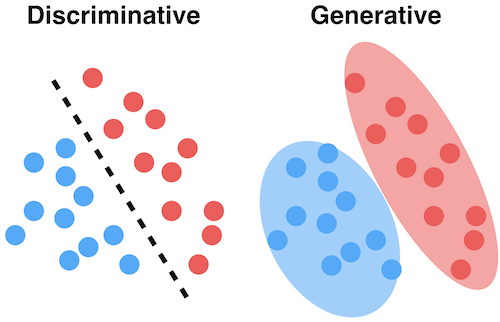
\includegraphics[width=0.5\textwidth]{
		images/01_Introduction_discriminativeAndGenerative.png
	}
	\caption{Discriminative \textit{vs} Generative Models}
	\label{descriminative_generative}
\end{figure}
    \chapter{Decision Trees}
\label{cha:decision_trees}

\begin{figure}[H]
	\centering
	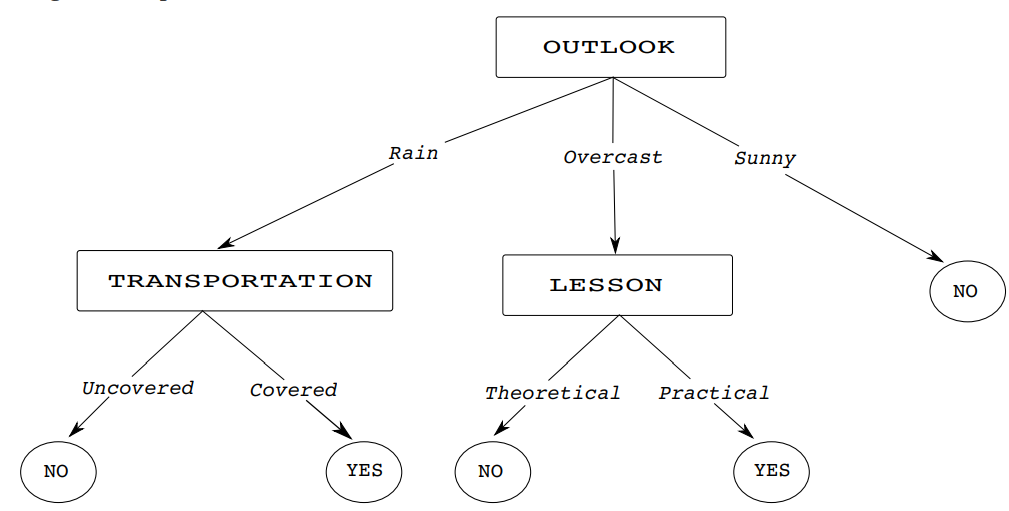
\includegraphics[width=0.8\textwidth]{
		images/02_DecisionTrees_decisionTree1.png
	}
	\caption{Toy example of a decision tree. \textit{Go to lesson}.}
	\label{dt_example}
\end{figure}

\defi{\textbf{Decision tree} \label{def:dt}\\ A \textit{decision tree} encodes a logical formula expressed in \textit{disjunctive normal form}. It consists of a disjunction of conjuctions of constraints over attribute values. Each path from the root to a leaf is a conjunction of the constraints specified in the nodes along it. The leaf contains the label to be assigned to instances reaching it. }
Given a decision three, such as the one reported in Figure \ref{dt_example}, the
disjunction of all paths is the logical formula represented by the tree.

% \begin{equation*}
% \begin{array}{l}
%     (\mathit{OUTLOOK}=\mathit{Rain} \wedge \mathit{TRANSPORTATION}=\mathit{Covered})\\
%     \vee \\
%     (\mathit{OUTLOOK}=\mathit{Overcast} \wedge \mathit{LESSON}=\mathit{Practical})
% \end{array}
% \end{equation*}

\begin{gather*}
	(\mathit{OUTLOOK}=\mathit{Rain}\wedge \mathit{TRANSPORTATION}=\mathit{Covered})
	\\ \vee \\ (\mathit{OUTLOOK}=\mathit{Overcast}\wedge \mathit{LESSON}=\mathit{Practical}
	)
\end{gather*}

\textbf{Remark:} the tree encodes a DNF formula for each class.
\newline

Appropriate problems for decision trees are:
\begin{itemize}
	\item Binary or multiclass classification tasks. Extensions to regressions
		also exists. The most simple regression extension is to predict the average of
		the training examples which reached a leaf.

	\item Instances represented as attribute-value pairs. Indeed the idea is to
		split according to attribute values.

	\item Different explanations for the concept are possible (disjunction). For
		example looking at decision tree in Figure \ref{dt_example}, there can be several
		reasons why I decide to attend a lecture. Decision trees allow to learn
		several explanations for a given concept.

	\item Some instances have missing attributes, i.e. for some attributes we do not
		have the value. This is typical in medical domain in which it is unlikely
		that a patient did all the possible tests which could be useful to make a
		prediction.

	\item There is need for an interpretable explanation of the output.
\end{itemize}

\begin{figure}[H]
	\centering
	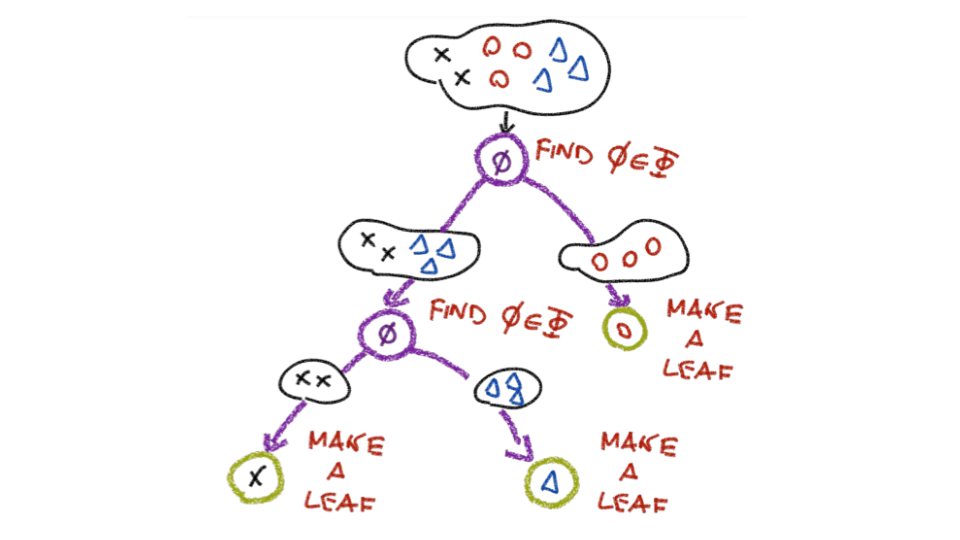
\includegraphics[width=0.7\textwidth]{
		images/02_DecisionTrees_decisionTree2.png
	}
	\caption{Split node training set into children according to the value of the
	chosen attribute}
	\label{ricci_dt}
\end{figure}

\section{Learning decision trees}
In order to learn a decision tree, we follow a \textit{greedy} top-down strategy
inspired by a \textit{divide et impera} approach. For each node, starting from the
root with full training set:
\begin{enumerate}
	\item Choose the best attribute to be evaluated

	\item Add a child for each attribute value

	\item Split node training set into children according to the value of the chosen
		attribute

	\item Stop splitting a node when a stopping condition is met. For example, the
		node which has been reached contains examples from a single class (all
		examples have the same label, they are homogeneous), or there are no more attributes
		to test.
\end{enumerate}

\textbf{Remark:} if the current set of examples is not homogeneous but we stop
splitting for other reasons, we assign to the leaf the majority class of the set.
\newline

In essence, the learning algorithm recursively partitions the training set and
decides whether to grow leaves or non-terminal nodes.

\subsection{Choosing the best attribute}

\defi{\textbf{Entropy} \label{def:entropy}\\ The \textit{entropy} is a measure of the amount of information contained in a collection of instances (training examples) $S$ which can take a number $c$ of possible values (class labels). The entropy of a set of labelled examples measures its label inhomogeneity. \begin{equation}H(S) = - \sum_{i=1}^{c}p_{i}\log_{2}{p_i}\end{equation} where $p_{i}$ is the fraction of $S$ taking value $i$. }

\defi{\textbf{Information gain} \label{def:information_gain}\\ \textit{Information gain} is the expected reduction of entropy obtained by partitioning a set $S$ according to the value of a certain attribute $A$. \begin{equation}\mathit{IG}(S,A) = H(S)-\sum_{v \in \mathit{Values}(A)}\frac{|S_{v}|}{|S|}H(S_{v})\end{equation} where $\mathit{Values}(A)$ is the set of possible values taken by $A$ and $S_{v}$ is the subset of $S$ taking value $v$ at attribute $A$. \begin{itemize}\item The second term represents the sum of entropies of subsets of examples obtained partitioning over $A$ values, weighted by their respective sizes.

\item An attribute with high information gain tends to produce homogeneous groups in terms of labels, thus favouring their classification.\end{itemize} \textbf{Remark:} \[IG(S,A) \geq 0\] }

Overall, the selection of the best splitting attribute is given in terms of
maximization of information gain. The procedure ends when the subset of the training
set which has reached a given node along the path from the root of the tree satisfies
a certain criterion. For instance, the set of training examples which has reached
the current node, is characterized by a homogeneity value lower then a given
threshold ($H(S)<\epsilon$), has a given minimum cardinality ($|S|<k$), is
completely homogeneous, there are no more splitting attributes to choose.
Depending on the particular implementation, in some of these cases we grow a leaf
instead of splitting the training examples and generating new intermediate nodes.

\section{Issues in decision tree learning}

\subsection{Overfitting avoidance}
Decision trees have a structure that is determined by the data. As a result they
are flexible and can easily fit the training set, with high risk of overfitting.\\
Requiring that each leaf has only examples of a certain class can lead to very
complex trees. A complex tree can easily overfit the training set, incorporating
random regularities not representative of the full distribution. What is more many
kinds of noise can occur in the training data: some values of attributes are
incorrect because of errors in the data acquisition process, the instance was labeled
incorrectly, some attributes are irrelevant to the decision making process. In order
to build simpler tree structures, less prone to overfitting, it is possible to accept
impure leaves, assigning them the label of the majority of their training
examples.\\ A technique to reduce complexity is called \textit{pruning}. There
are two possible strategies to prune a decision tree:
\begin{itemize}
	\item \textbf{pre-pruning}: decide whether to stop splitting a node even if it
		contains training examples with different labels.

	\item \textbf{post-pruning}: learn a full tree and successively prune it removing
		subtrees, replacing whole subtrees with leaf nodes.
\end{itemize}

With the aim of improving generalization and as a consequence, reducing overfitting,
if a \textit{validation set} is available it is possible to implement a post-pruning
strategy. The procedure is described in Algorithm \ref{alg:postPruning}.

\begin{algorithm}
	\caption{Post pruning \label{alg:postPruning}}
	\begin{algorithmic}
		[1] \STATE \textbf{for each} node $n$ in the tree \textbf{do}\{ \STATE \tab
		Evaluate the performance on the validation set \STATE \tab when removing the
		subtree rooted at $n$ \STATE \} \STATE \textbf{if} all node removals worsen performance\{
		\STATE \tab STOP \STATE \} \STATE \STATE $n$ $\leftarrow$ node whose removal
		has the best performance improvement \STATE \STATE Replace the subtree
		rooted at $n$ with a leaf \STATE \STATE Assign to the leaf the majority
		label of all examples in the subtree \STATE \STATE \textbf{return} to line 1
	\end{algorithmic}
\end{algorithm}

\subsection{Dealing with continuous-valued attributes}
Continuous valued attributes need to be discretized in order to be used in internal
nodes tests. Discretization threshold can be chosen to maximize the information
gain. A possible procedure is the following:
\begin{enumerate}
	\item Examples are sorted according to their continuous attribute values.

	\item For each pair of successive examples having different labels, a
		candidate threshold is placed as the average of the two attribute values.

	\item For each candidate threshold, the information gain achieved by splitting
		the examples is computed.

	\item The threshold producing the higher information gain is used to discretize
		the attribute.
\end{enumerate}

\subsection{Alternative attribute test measures}
The information gain criterion tends to prefer attributes with a large number of
possible values. As an extreme, the unique ID of each example is an attribute which
perfectly splits the data into singletons, but it will be of no use on new
examples. Moreover, this would lead to overfitting.
\paragraph{}
In order to deal with this problem a new measure of entropy is introduced. In this
case we do not compute entropy taking into account class values, but we
calculate the spread with respect to the values of the attributes.
\begin{equation}
	H_{A}(S) = -\sum_{v \in \mathit{Values}(A)}\frac{|S_{v}|}{|S|}\log_{2}{\frac{|S_{v}|}{|S|}}
\end{equation}
This quantity is maximized when there exists an attribute which splits the dataset
homogeneously in many subsets. The aim is to discourage the choice of these kind
of attributes to perform the splits. To do this \textit{gain ratio} is
introduced as an alternative of information gain measure introduced above.
\begin{equation}
	\mathit{IGR}(S,A) = \frac{\mathit{IG}(S,A)}{H_{A}(S)}
\end{equation}
In this case, splitting according to unique identifiers would result in high
values of entropy with respect to attribute values ($H_{A}(S)$), which leads to low
values of gain ratio ($\mathit{IGR}(S,A)$).

\subsection{Handling attributes with missing values}
Assume that an example $x$ with class $c(x)$ has missing value for attribute $A$.
When attribute $A$ has to be tested at node $n$, the following solutions could be
adopted:
\begin{itemize}
	\item \textit{Simple solution}. Assign to $x$ the most common attribute value among
		the examples in $n$ or (during training) the most common attribute value among
		the examples in $n$ with class $c(x)$.

	\item \textit{Complex solution}. Propagate $x$ to each of the children of $n$,
		with a fractional value equal to the proportion of examples with the
		corresponding attribute value.\\At training time, you assign the leaf the
		majority vote among the training examples which reach that leaf considering
		their weight.\\At test time, if we process an example with missing
		attributes it ends up in multiple leaves with a given probability. Each leaf
		votes with a weight which depends on the fraction of the test example which reached
		that leaf.
\end{itemize}

\begin{figure}[H]
	\centering
	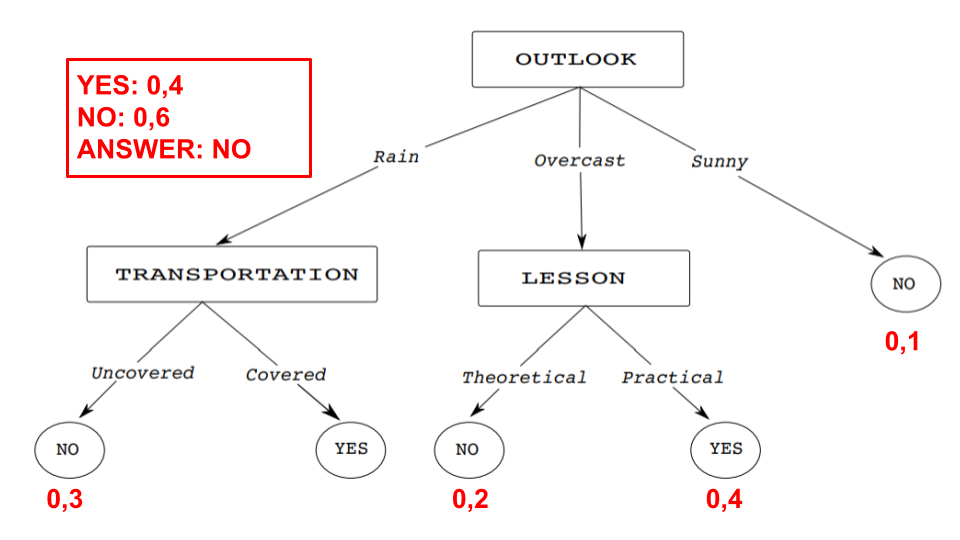
\includegraphics[width=0.8\textwidth]{
		images/02_DecisionTrees_missingAttributes.png
	}
	\caption{Dealing with missing attributes at test time. Complex solution.}
	\label{missing_attributes}
\end{figure}

\section{Random forest}

A common technique to reduce overfitting is \textit{ensemble learning}. Following
this method we learn multiple models at training time. At test time we average
the results or take the majority vote of the models.

\subsection{Bootstrap sampling and bagging}
\paragraph{}
\textbf{Bootstrap sampling:} Given a set $D$ containing $N$ training examples, create
$D'$ by drawing $N$ examples at random with replacement (i.e. same example can be
selected multiple times) from $D$.
\paragraph{}
\textbf{Bagging:}
\begin{enumerate}
	\item Create $k$ bootstrap datasets $D_{i}$

	\item Train distinct classifier on each $D_{i}$

	\item Classify new instance by majority vote/average
\end{enumerate}

\subsection{Training}
Random forests are ensembles of decision trees. Each tree is typically trained on
a bootstrapped version of the training set (sampled with replacement, i.e.
independent samples). Each decision tree is independently trained with its
bootstrapped version of the training set. At each node the splitting function is
optimized on $m$ randomly sampled features. This helps obtaining decorrelated
decision trees At the end of the training a forest with $M$ trees is generated.
\begin{figure}[H]
	\centering
	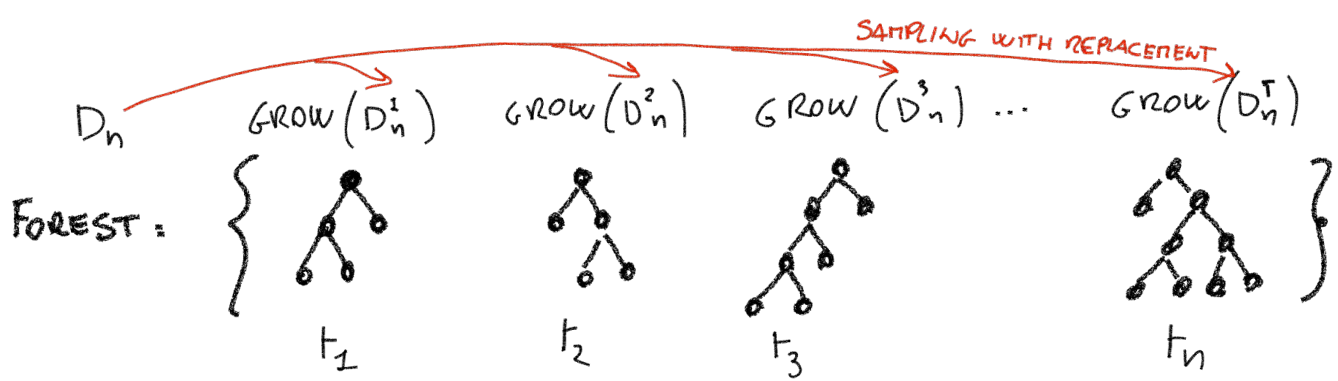
\includegraphics[width=\textwidth]{images/02_DecisionTrees_randomForest.png}
	\caption{Random forest}
	\label{rf}
\end{figure}

\subsection{Testing}
\begin{enumerate}
	\item Test the example with each tree in the forest.

	\item Return the majority class among the predictions.
\end{enumerate}
More formally, given a set of trees $Q=\{t_{1}, ..., t_{T}\}$, the final
prediction of the forst is obtained by averaging the prediction of each tree in
the ensemble:
\begin{equation}
	f_{Q}(x) = \frac{1}{T}\sum_{j=1}^{T}f_{t}(x)
\end{equation}
    \chapter{K-nearest neighbors}
\label{cha:KNN}

\defi{\textbf{K-Nearest Neighbors (kNN)} \label{def:knn}\\
K-nearest neighbors algorithm is a non-parametric supervised learning method. It allows to define the belonging of an example to an area of influence of the data used for learning.
}

\textbf{Remark:} kNN is non-parametric since it does not make any assumptions on the data being studied, i.e., the model is distributed from the data. \newline

\textbf{Remark:} kNN is a lazy algorithm because it does not use the training data points to make any generalisation. Which implies: \begin{itemize}
    \item You expect little to no explicit training phase,
    \item The training phase is pretty fast,
    \item kNN keeps all the training data since they are needed during the testing phase.
\end{itemize}

Given a training set, each point has its own area of influence, as the area in which is most likely to position new samples that can be labelled as the main point.
Training data can be positioned in a multidimensional space, so the concept of distance we use is not the "trivial" one: euclidean distance is not always the best option. 
The $k$ in \textbf{kNN} means that the number of closest neighbors we consider is equal to $k$ (e.g. if $k=3$ and two of them are points of a class A and only one belongs to a class B, then the point we are trying to classify will belong to class A, regardless of the position of the three points in training set).\\

\defi{\textbf{Concept of distance (or metric)} \label{defi:distance}\\
Given a set $\mathcal{X}$ a function $d:\mathcal{X} \times \mathcal{X} \rightarrow \R^{+}_{0}$ is a metric for $\mathcal{X}$ if for any $x, y, z \in \mathcal{X}$ the following proprieties are satisfied:
\begin{itemize}
    \item \textbf{reflexivity}: $d(x, y)=0 \Leftrightarrow x=y$
    \item \textbf{symmetry}: $d(x, y) = d(y, x)$
    \item \textbf{triangle inequality}: $d(x, y) + d(y, z) \geq d(x, z)$
\end{itemize}
}

An example of a metric distance definition is the euclidean distance:\\

$$d(x, y) = \sqrt{\sum_{i=1}^n (x_{i} - y_{i})^{2}}$$

The pseudo-algorithm for classification problems \ref{def:binary_classification} \ref{def:multiclass_classification} \ref{def:multilabel_classification} can be formalized with Algorithm \ref{alg:knn_classification}. 

\begin{algorithm}
\caption{kNN for classification \label{alg:knn_classification}}
\begin{algorithmic}
\FORALL{test examples $x$} 
    \FORALL {training examples $(x_i, y_i)$}
        \STATE compute distance $d(x, x_i)$
    \ENDFOR
    \STATE select the k-nearest neighbors\\
    \RETURN class of x as majority class among k-neighbors
\ENDFOR
\end{algorithmic}
\end{algorithm}

The selection of the majority vote can be formalized as:\\

\begin{equation}
    argmax_y {\sum_{i=1}^k \delta(y, y_{i})}
\end{equation}

The pseudo-algorithm for regression problems \ref{def:regression} can be formalized with Algorithm \ref{alg:knn_regression}. 

\begin{algorithm}
\caption{kNN for regression \label{alg:knn_regression}}
\begin{algorithmic}
\FORALL{test examples $x$} 
    \FORALL {training examples $(x_i, y_i)$}
        \STATE compute distance $d(x, x_i)$
    \ENDFOR
    \STATE select the k-nearest neighbors\\
    \RETURN the average output value among neighbors
\ENDFOR
\end{algorithmic}
\end{algorithm}

The computation of the average value can be formalized as:\\

$$\frac{1}{k} \sum_{i=1}^k y_{i}$$

\section{Characteristic of kNN learning}
    Here are reported the main features of the kNN algorithm:
    \begin{itemize}
        \item \textbf{instance-based learning}: the models results calibrated for the test example to be processed.\\
        \textit{Instance-based learning} (sometimes called \textit{memory-based learning}) is a family of learning algorithms that, instead of performing explicit generalization, compare new problem instances with instances seen in training, which have been stored in memory. In other words, this methods construct hypotheses directly from the training instances themselves. This means that the hypothesis complexity can grow with the data: in the worst case, a hypothesis is a list of $n$ training items and the computational complexity of classifying a single new instance is $\mathcal{O}(n)$. One advantage that instance-based learning has over other methods of machine learning is its ability to adapt its model to previously unseen data. Instance-based learners may simply store a new instance or throw an old instance away.\\Because computation is postponed until a new instance is observed, these algorithms are sometimes referred to as \textit{lazy}. 
        \item \textbf{lazy learning}: computation is mostly deferred to the classification phase (speed up research)
        \item \textbf{local learner}: assumes prediction should be mainly influenced by nearby instances (an area is affected by a class)
        \item \textbf{uniform feature weighting}: all features are uniformly weighted in computing distances, no data point or distance affect the classification in any way since the given data point in the training set is considered in the set of nearest neighbours.
    \end{itemize}
    
    Anyhow, for the last point, a further implementation of the \textit{kNN algorithm} is available: its upgrade consists in giving the data a different weight proportional to the inverse of the distance.\\
    
    For the classification problem, the selection of the majority vote is: 
    \begin{equation}
        argmax_y {\sum_{i=1}^k w_{i}\delta(y, y_{i})}
    \end{equation}
    
    while for the regression problem is:
    \begin{equation}
        \frac{ {\sum_{i=1}^k w_{i}y_{i}}}
        { {\sum_{i=1}^k w_{i}}}
    \end{equation}    
    
    where 
    
    \begin{equation}
        w_{i} = \frac{1}{d(x, x_{i})}
    \end{equation}    
    
    \chapter{Linear algebra}
\label{cha:linear_algebra} \defi{\textbf{Group} \label{def:group}\\In abstract algebra, a group is a set $G$ where an operation $*$ is defined. Moreover $*$ satisfies the following properties: \begin{enumerate}\item \textit{associative}: $(a*b)*c=a*(b*c) \forall a,b,c \in G$

\item \textit{identity element}: $\exists e \in G : a*e=e*a=a \forall a \in G$

\item \textit{inverse element}: $\forall a \in G$ $\exists a' \in G : a*a'=a'*a=e$\end{enumerate} }

\defi{\textbf{Commutative group} \label{def:comm_group}\\ A group $(G,*)$ is \textit{commutative} iff $a*b=b*a$ $\forall a,b \in G$. }

\defi{\textbf{Vector space} \label{def:vector_space}\\ A \textit{vector space} over the field $\mathcal{R}$ is an algebraic structure composed by a commutative group $(V,+)$, whose elements are called $vectors$, and a function $f:\mathcal{R}\times V \rightarrow V$ called \textit{scalar multiplication} which satisfies the properties listed below. It is common to use $kv$, instead of $f(k,v)$ to represent the scalar multiplication between a scalar $k \in \mathcal{R}$ and a vector $v \in V$. \begin{itemize}\item \textit{distributive over elements} $k(v_{1}+v_{2})=kv_{1}+kv_{2}$

\item \textit{distributive over scalars} $(k_{1}+k_{2})v=k_{1}v+k_{2}v$

\item \textit{associative over scalars} $(k_{1}k_{2})v=k_{1}(k_{2}v)$

\item \textit{identity element} $1v=v$\end{itemize} $\forall k,k_{1},k_{2}\in \mathcal{R}, \forall v, v_{1}, v_{2}\in V$. }
Vector space examples are: the set of two-dimensional vectors $V^{2}$, the set
of three-dimensional vectors $V^{3}$, the matrix space $M_{m,n}(\mathcal{R})$.

\defi{\textbf{Subspace} \label{def:subspace}\\ Given a vector space $V$ defined over the field $R$, a non-empty set $W \subseteq V$ is a \textit{subspace} of $V$ if it is close w.r.t. the sum of vectors and the scalar product: \begin{equation*}\forall w,w'\in W, \forall k \in K, w+w' \in W \wedge kw \in W\end{equation*} Each subspace is in turn a vector space with respect to the operations defined in $V$. }

\defi{\textbf{Linear combination} \label{def:linear_combination}\\ Given a vector $v \in V$, $v$ is a linear combination of the vectors $v_{1},...,v_{k}\in V$ with coefficients $c_{i}\in \mathcal{R}$ if: \begin{equation*}v = c_{1}v_{1}+...+c_{k}v_{k}= \sum_{i=1}^{K}c_{i}v_{i}\end{equation*} }

\defi{\textbf{Span} \label{def:span}\\ The span of vectors $v_{1},...,v_{k}$ is defined as the set of their linear combinations: \begin{equation*}\{\sum_{i=1}^{K}c_{i}v_{i}, c_{i}\in \mathcal{R}\} = <v_{1},...,v_{k}>\end{equation*} The span is a \textit{vector subspace} (also known as \textit{linear subspace}) of $V$. In particular the span $<v_{1},...,v_{k}>$ is the subset generated by $v_{1},...,v_{k}$. }

\defi{\textbf{Linear independency and linear dependency} \label{def:indipendency1}\\ A set of vectors $v_{1},...,v_{k}$ is \textit{linearly independent} if the null vector can be written as a linear combination of the elements $v_{i}$ of the set

\begin{equation*}a_{1}v_{1}+a_{2}v_{2}+...+a_{k}v_{k}=0\end{equation*}

if and only if all the coefficients $a_{1},...,a_{k}$ are null. Intuitively, a set of vectors $v_{1},...,v_{k}$ is linearly independent if none of them can be written as a linear combination of the others. \\ A set of vectors $v_{1},...,v_{k}$ is \textit{linearly dependent} is it is not linearly independent. As a consequence, a set of vectors $v_{1},...,v_{k}$ is linearly dependent if there exist some not-null scalars $a_{1},...,a_{k}$ such that: \begin{equation*}a_{1}v_{1}+a_{2}v_{2}+...+a_{k}v_{k}=0\end{equation*} }

\defi{\textbf{Basis} \label{def:basis1}\\ A set of vectors $\mathcal{B}=\{v_{1},...,v_{k}\}$ is a \textit{basis} for $V$ if any element in $V$ can be uniquely written as a linear combination of vectors $v_{i}$. A necessary condition is that vectors $v_{i}$ are linearly independent. All bases of $V$ have the same number of elements, called the \textit{dimension} of the vector space. }
\defi{\textbf{Linear maps} \label{def:linear_maps}\\ Given two vector spaces $V$ and $V'$, a function $f: V \rightarrow V'$ is a \textit{linear map} if $\forall a_{1}, a_{2}\in \mathcal{R}, v_{1}, v_{2}\in V$: \begin{equation*}f(a_{1}v_{1}+a_{2}v_{2})=a_{1}f(v_{1})+a_{2}f(v_{2})\end{equation*} }

A linear map between two finite-dimensional spaces $V$, $V'$ of dimensions $n$,$m$
can always be written as a matrix $A$. Consider a linear map
$T: V \rightarrow V'$ and two sets $\mathcal{B}=\{u_{1},...,u_{n}\}$, $\mathcal{C}
=\{v_{1},...,v_{m}\}$ which are basis of $V$ and $V'$ respectively.

Consider also two isomorphisms $T_{\mathcal{B}}: V \rightarrow{\mathcal{R}}^{n}$,
$T_{\mathcal{C}}: V' \rightarrow{\mathcal{R}}^{m}$ which associate to each
vector its coordinates with respect to a given base. These two isomorphisms uniquely
identify a matrix $A \in M_{m,n}(\mathcal{R})$. The $n$ columns of $A$ are the
vectors $T_{\mathcal{C}}(T(u_{j}))$ obtained from the coordinates of the images
$T(u_{1}),...,T(u_{n})$, with respect to basis $\mathcal{C}$.

For any $x \in V$ we have:
\begin{itemize}
	\item Each element $x \in V$ can be written as a linear combination of the elements
		of the basis $\mathcal{B}$.
\end{itemize}
\begin{equation*}
	f(x) = f(\sum_{i=1}^{n}\lambda_{i}u_{i}) = \sum_{i=1}^{n}\lambda_{i}f(u_{i})
\end{equation*}
\begin{itemize}
	\item Given that the $n$ columns of $A$ are the vectors $T_{\mathcal{C}}(T(u_{j}
		))$ obtained from the coordinates of the images $T(u_{1}),...,T(u_{n})$,
		with respect to basis $\mathcal{C}$.
\end{itemize}
\begin{equation*}
	f(u_{i}) = \sum_{j=1}^{m}a_{ji}v_{j}
\end{equation*}
\begin{itemize}
	\item Putting all together we notice that actually the image of $f(x)$ can be written
		as a linear combination of the elements of the basis $\mathcal{C}$. As a
		consequence, $f(x)$ belongs to the vector space $V'$.
\end{itemize}
\begin{equation*}
	f(x) = \sum_{i=1}^{n}\lambda_{i}f(u_{i}) = \sum_{i=1}^{n}\sum_{j=1}^{m}\lambda_{i}
	a_{ji}v_{j}= \sum_{j=1}^{m}(\sum_{i=1}^{n}\lambda_{i}a_{ji}) v_{j}= \sum_{j=1}^{m}
	\mu_{j}v_{j}
\end{equation*}

The matrix $A \in M_{mn}(\mathcal{R})$ defined above is called the matrix associated
with the linear map $T$ with respect to the basis $\mathcal{B}$, $\mathcal{C}$. $A$
is typically indicated with the symbol $M^{\mathcal{C}}_{\mathcal{B}}(T)$. If
$V=V'$ and $\mathcal{B}=\mathcal{C}$, then we write $M_{\mathcal{B}}(T)$. If
$V=\mathcal{R}^{n}$, $V'=\mathcal{R}^{m}$ and we consider the canonical basis of
the two vector spaces, then we simply write $M(T)$.

Consider a linear map $T$ and a matrix $A=M^{\mathcal{C}}_{\mathcal{B}}(T)$
defined as described above. Consider also a vector $v \in V$ and a vector $x$.
This latter is the column vector of the coordinates $x_{1},...,x_{n}$ of $v$
with respect to the basis $\mathcal{B}$. Given that, the image of $T(v)$ has a
corresponding vector of coordinates with respect to basis $\mathcal{C}$ which
can be calculated by the matrix multiplication $Ax$. We propose an example in Figure~\ref{fig:linear_function_matrix}.
\begin{figure}[H]
	\centering
	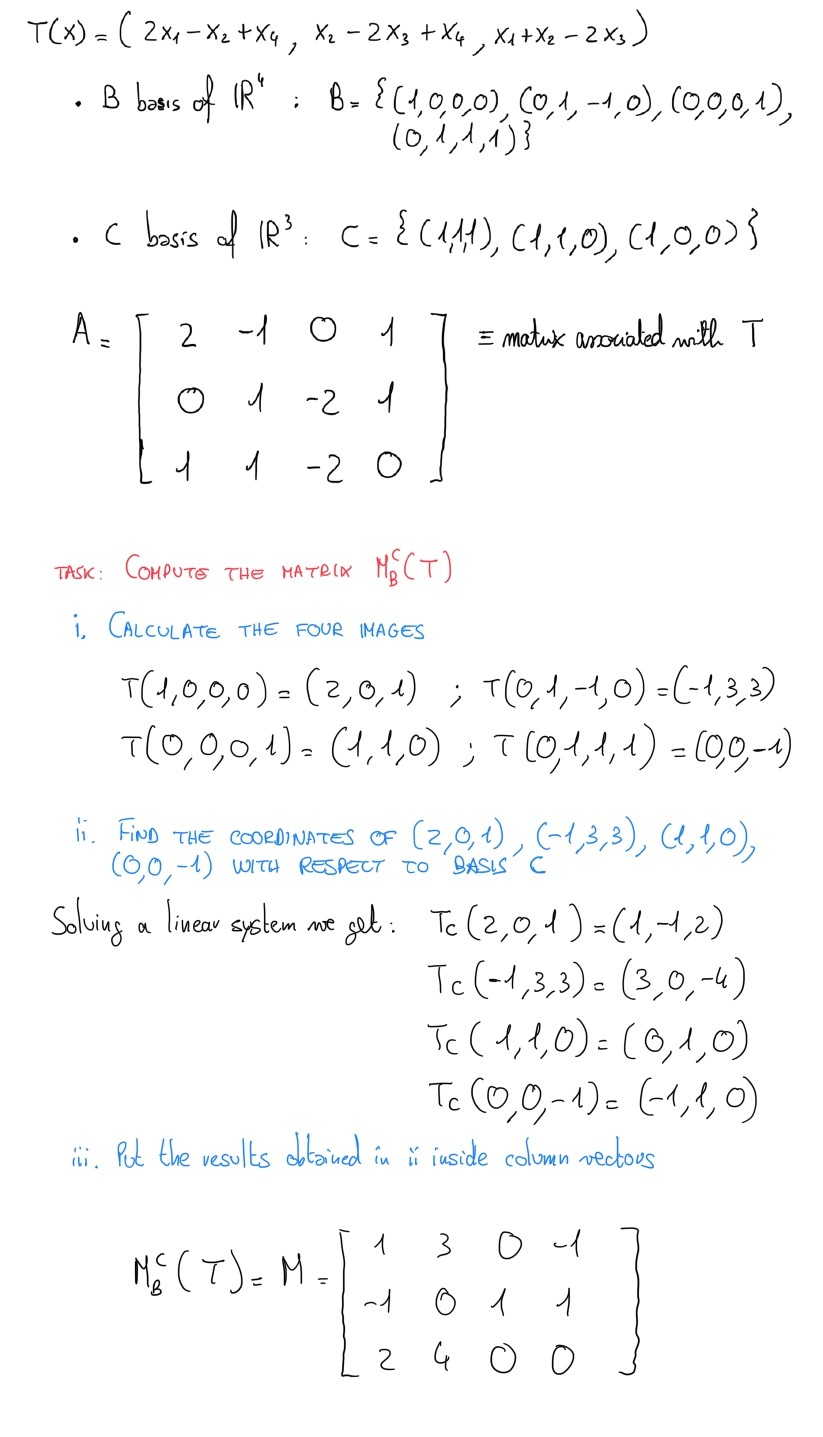
\includegraphics[scale=0.60]{images/04_LinearAlgebra_matrixLinearFunction.jpg}
	\caption{Example of a computation of the matrix associated with a linear
	function}
	\label{fig:linear_function_matrix}
\end{figure}

\defi{\textbf{Matrix of basis transformation} \label{def:basis_transformation}\\ Consider two basis of the vector space $V$: $\mathcal{B}=\{v_{1},...,v_{n}\}$ and $\mathcal{B}'=\{v'_{1},...,v'_{n}\}$. The \textit{transition matrix} (or \textit{matrix of basis transformation}) from $\mathcal{B}$ to $\mathcal{B}'$ is the invertible matrix $P=[p_{ij}]$, with order $n$, whose columns are the coordinates of the vectors $v_{j}$ of the basis $\mathcal{B}$ with respect to the basis $\mathcal{B}'$. \begin{equation*}v_{j}= \sum_{i}p_{ij}v'_{i}\quad (j = 1,...,n)\end{equation*} }

\textbf{Remark:} The matrix $P$ is the matrix associated with the identity
function with respect to the basis $\mathcal{B}$ and $\mathcal{B}'$ :
$P = M^{\mathcal{B}'}_{\mathcal{B}}(id_{V})$. From this observation we can derive
the following consequence. If the vector $v \in V$ has coordinates
$x_{1},...,x_{n}$ with respect to basis $\mathcal{B}$, and coordinates $x'_{1},..
.,x'_{n}$ with respect to basis $\mathcal{B}'$, then:
\begin{equation}
	x' = Px
\end{equation}
where $P$ is the matrix of basis transformation from $\mathcal{B}$ to $\mathcal{B}
'$. We propose an example of basis transformation in $\mathcal{R}^{2}$ in Figure
\ref{fig:basis_transformation}.

\begin{figure}[H]
	\centering
	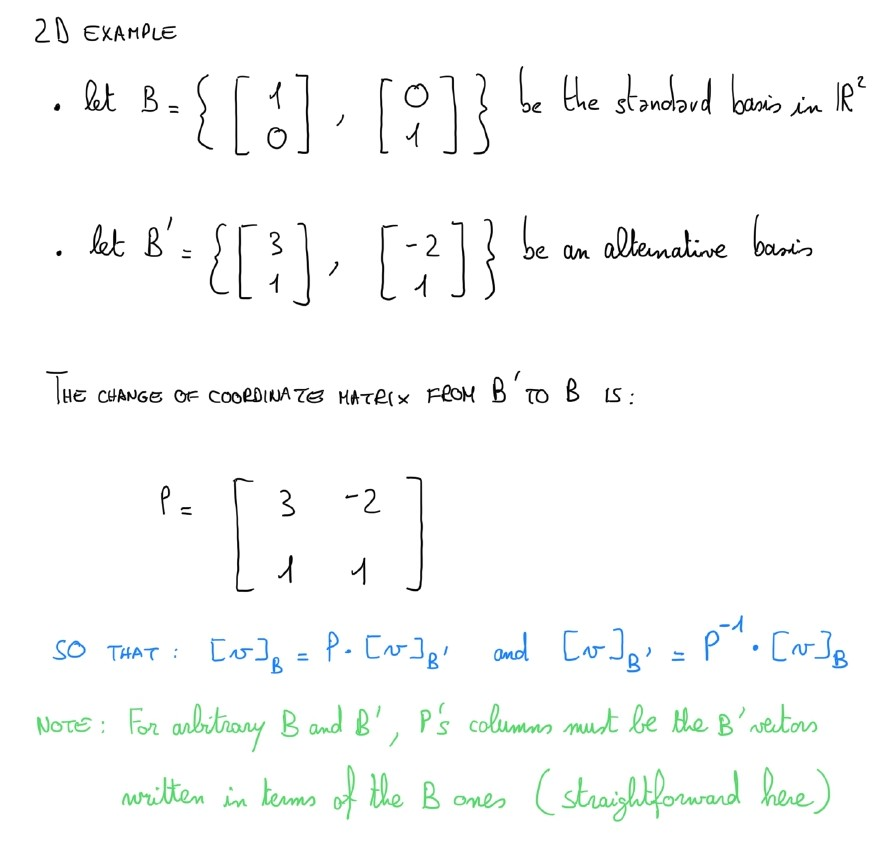
\includegraphics[scale=0.65]{images/04_LinearAlgebra_basisTransformation.jpg}
	\caption{2D example of basis transformation.}
	\label{fig:basis_transformation}
\end{figure}

\defi{\textbf{Transpose} \label{def:transpose}\\ Matrix obtained exchanging rows with columns (indicated with $M^{T}$).\\Given two matrices $M$,$N$ and their transposes $M^{T}$, $N^{T}$, the following relevant property holds: \begin{equation*}(MN)^{T}= N^{T}M^{T}\end{equation*} }

\defi{\textbf{Trace} \label{def:trace}\\ Sum of diagonal elements of a matrix. \begin{equation*}tr(M) = \sum_{i=1}^{n}M_{ii}\end{equation*} }

\defi{\textbf{Inverse} \label{def:inverse}\\ The matrix which multiplied with the original matrix gives the identity. \begin{equation*}MM^{-1}=I\end{equation*} }

\defi{\textbf{Rank} \label{def:rank}\\ The rank of a $n \times m$ matrix is the dimension of the space spanned by its columns. Consider a matrix $A$ $m \times n$. In the matrix there are $n$ columns $A^{1},...,A^{n}$. It is possible to demonstrate that the column space $<A^{1},...,A^{n}>$ has dimension equal to the rank of the matrix $A$. \begin{equation*}rg(A) = \mathit{dim}(<A^{1},...,A^{n}>)\end{equation*} In particular the columns of $A$ are linearly independent if and only if $rg(A)=n$. }

\section{Matrix derivatives}
In this section, there are reported some useful properties of matrix calculus.

\begin{equation*}
	\centering
	\begin{aligned}
		\frac{\partial M \mathbf{x}}{\partial \mathbf{x}}              & =M                                                              \\
		\frac{\partial \mathbf{y}^T M \mathbf{x}}{\partial \mathbf{x}} & =M^{T} \mathbf{y}                                               \\
		\frac{\partial \mathbf{x}^T M \mathbf{x}}{\partial \mathbf{x}} & =\left(M^{T}+M\right) \mathbf{x}                                \\
		\frac{\partial \mathbf{x}^T M \mathbf{x}}{\partial \mathbf{x}} & =2 M \mathbf{x}\quad \text{ if }\mathbf{M}\text{ is symmetric } \\
		\frac{\partial \mathbf{x}^T \mathbf{x}}{\partial \mathbf{x}}   & =2 \mathbf{x}
	\end{aligned}
\end{equation*}

\textbf{Note:} Results are column vectors. Transpose them if row vectors are needed
instead.

\section{Metric structure}
\defi{\textbf{Norm} \label{def:norm}\\ The \textit{norm} defined in $\mathcal{R}^{n}$ is a function $||\cdot||:\mathcal{X}\rightarrow \mathcal{R}_{0}^{+}$ which associates to the vector $x$ the non-negative real number: \begin{equation}||x|| = \sqrt{x \cdot x}= \sqrt{x_{1}^{2}+ ... + x_{n}^{2}}\end{equation} The norm has the following properties: \begin{itemize}\item $||x+y|| \leq ||x|| + ||y||$

\item $||\lambda x|| = |\lambda| ||x||$

\item $||x||>0$ if $x \neq 0$\end{itemize} where $x,y \in \mathcal{X}$, $\lambda \in \mathcal{R}$ }

\defi{\textbf{Metric} \label{def:metric}\\ A norm defines a \textit{metric} $d: \mathcal{X}\times \mathcal{X}\rightarrow \mathcal{R}_{0}^{+}$ such that: \begin{equation}d(x,y) = ||x-y||\end{equation} This metric is commonly referred to as $distance$. This latter is a function which associates to each couple of vectors $x,y \in \mathcal{R}^{n}$ the real number $d(x,y)$. }

\textbf{Remark:} The concept of norm is stronger than that of metric: not any metric
gives rise to a norm.\\

\defi{\textbf{Unit vector} \label{def:unit_vector}\\ A \textit{unit vector} is a vector $v \in \mathcal{R}^{n}$ such that: \begin{equation*}||v|| = 1\end{equation*} }

\textbf{Remark:} each vector $v \neq \pmb{0}$ can be normalized:
\begin{equation*}
	v' = \frac{v}{||v||}
\end{equation*}
where $v'$ is a unit vector.

\section{Dot product}
\defi{\textbf{Bilinear form} \label{def:bilinear_form}\\ A function $Q: \mathcal{X}\times \mathcal{X}\rightarrow \mathcal{R}$ on a vector space $X$ is a \textit{bilinear form} if it is linear in each argument separately: \begin{equation*}Q(\lambda x + \mu y, z) = \lambda Q(x,z) + \mu Q(y,z)\end{equation*}

\begin{equation*}Q(x, \lambda y + \mu z) = \lambda Q(x,y) + \mu Q(x,z)\end{equation*} where $x,y,z \in \mathcal{X}$, $\lambda, \mu \in \mathcal{R}$.

A bilinear form is \textit{symmetric} if for all $x,y \in \mathcal{X}$: \begin{equation*}Q(x,y) = Q(y,x)\end{equation*}

}

\defi{\textbf{Dot product} \label{def:dot_product}\\ The \textit{dot product} on $\mathcal{R}^{n}$ is a function $<\cdot,\cdot>: \mathcal{X}\times \mathcal{X}\rightarrow \mathcal{R}$ which associate to a couple of vectors $x,y \in \mathcal{R}^{n}$ the real number: \begin{equation}<x,y> = x \cdot y = \sum_{i=1}^{n}x_{i}y_{i}= x^{T}y\end{equation} }

The dot product has the following properties:
\begin{enumerate}
	\item \textit{symmetric}: $x \cdot y = y \cdot x$ for all $x,y \in \mathcal{R}^{n}$

	\item \textit{bilinear}: $(\alpha x + \beta y) \cdot z = \alpha (x \cdot z) + \beta
		(y \cdot z)$ and $x \cdot (\alpha y + \beta z) = \alpha (x \cdot y) + \beta (
		x \cdot z)$, for all $x,y,z \in \mathcal{R}^{n}$ and
		$\alpha, \beta \in \mathcal{R}$

	\item \textit{symmetric bilinear}: this property follows from the previous ones

	\item \textit{positive semi-definite}: $x \cdot x \geq 0$ for all $x \in \mathcal{R}
		^{n}$

	\item The dot product could also be \textit{positive definite} if it satisfies:
		$x \cdot x = 0$ iff $x=0$ for all $x \in \mathcal{R}^{n}$
\end{enumerate}

Any dot product defines a corresponding \textit{norm} via:
\begin{equation*}
	||x|| = \sqrt{<x,x>}
\end{equation*}

\begin{itemize}
	\item The angle $\theta$ between two vectors is defined as:
\end{itemize}
\begin{equation}
	\cos{\theta}= \frac{<x,z>}{||x||||z||}
\end{equation}

\begin{itemize}
	\item Two vectors are \textit{orthogonal} if $<x,y>=0$.

	\item A set of vectors $\{x_{1},...,x_{n}\}$ is orthonormal if all vectors $x_{i}$
		in the set are mutually orthogonal and are all unit vectors:
\end{itemize}
\begin{equation*}
	<x_{i}, x_{j}> = \delta_{ij}
\end{equation*}
\hspace{7mm} where $\delta_{ij}=1$ if $i=j$, $0$ otherwise.

\section{Eigenvalues and eigenvectors}
\label{sec:eigenvalues_eigenvectors}

\defi{\textbf{Eigenvalues and eigenvectors} \label{def:eigen}\\ Given a $n \times n$ matrix $M$, the real value $\lambda$ and (non-zero) vector $x$ are an \textit{eigenvalue} and corresponding \textit{eigenvector} of $M$ if: \begin{equation}Mx=\lambda x\end{equation} }

\textbf{Properties:}
\begin{itemize}
	\item A $n \times n$ matrix has $n$ eigenvalues

	\item A $n \times n$ matrix can have less than $n$ distinct eigenvalues

	\item A $n \times n$ matrix can have less than $n$ linear independent eigenvectors
		(also fewer then the number of distinct eigenvalues)
\end{itemize}

\defi{\textbf{Singular matrices} \label{def:singular_matrix}\\ A matrix is \textit{singular} if it has a zero eigenvalue. \begin{equation*}Mx = 0x = 0\end{equation*} }

A singular matrix has linearly dependent columns (see Definition \ref{def:indipendency1}):
\begin{equation*}
	[M_{1}... M_{n-1}M_{n}]
	\begin{bmatrix}
		x_{1}   \\
		x_{2}   \\
		\vdots  \\
		x_{n-1} \\
		x_{n}
	\end{bmatrix}
	= 0
\end{equation*}
\begin{equation*}
	M_{1}x_{1}+\hdots+M_{n-1}x_{n-1}+M_{n}x_{n}= 0
\end{equation*}
\begin{equation*}
	M_{n}= M_{1}\frac{-x_{1}}{x_{n}}+\hdots+M_{n-1}\frac{-x_{n-1}}{x_{n}}
\end{equation*}

\defi{\textbf{Determinant} \label{def:determinant}\\ The \textit{determinant} $|M|$ of a $n \times n$ matrix $M$ is the product of its eigenvalues. }

\textbf{Remark:} a matrix is \textit{invertible} if its determinant is not zero
(i.e. it is not singular).

\defi{\textbf{Symmetric matrix} \label{def:symmetric_matrix}\\ A \textit{symmetric matrix} is a square matrix that is equal to its transpose. \begin{equation*}A = A^{T}\end{equation*} Because equal matrices have equal dimensions, only square matrices can be symmetric. The entries of a symmetric matrix are symmetric with respect to the main diagonal. So if $a_{ij}$ denotes the entry in the $i$th row and $j$th column then: \begin{equation*}a_{ji}= a_{ij}\end{equation*} for all indices $i$ and $j$. }

If A is a real symmetric matrix, then any two eigenvectors ($x,z$) corresponding
to distinct eigenvalues ($\lambda \neq \mu$) are orthogonal. $(x, \lambda)$ and $(
z, \mu)$ IF $\lambda \neq \mu \Rightarrow <x,z>=0$. The proof of this
preposition is reported in Figure \ref{fig:proof_eigen_symmetric}.

\begin{figure}[H]
	\centering
	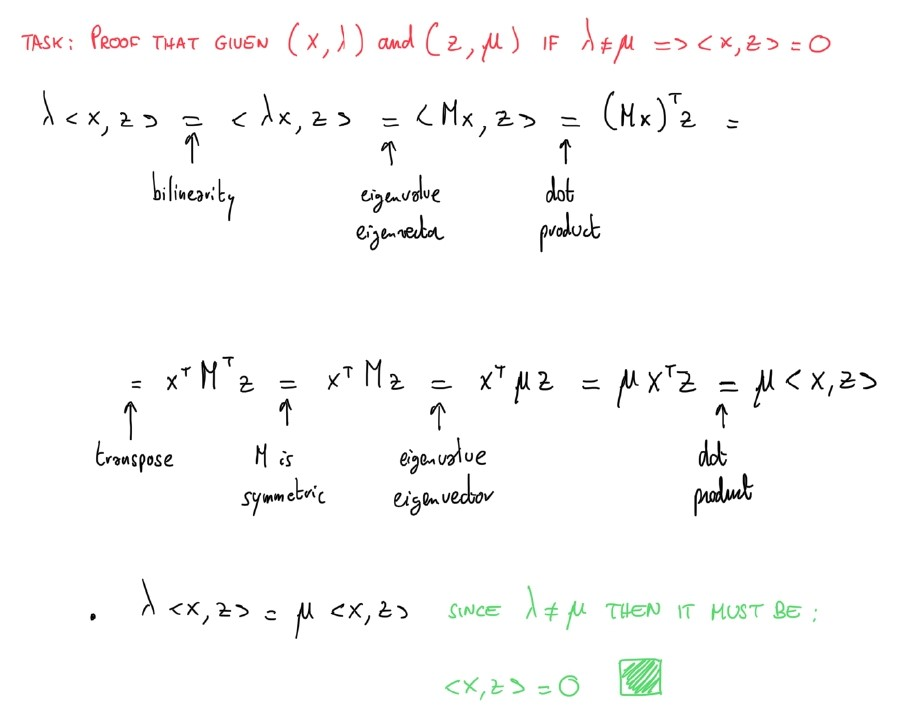
\includegraphics[scale=0.85]{images/04_LinearAlgebra_symmetricMatrixProof.jpg}
	\caption{Proof that $(x, \lambda)$ and $(z, \mu)$ IF
	$\lambda \neq \mu \Rightarrow <x,z>=0$.}
	\label{fig:proof_eigen_symmetric}
\end{figure}

\section{Eigen-decomposition}
The purpose of this section is to describe an iterative procedure to find eigenvalues
and eigenvectors for a matrix $A$. Given $A$ we want to find $\lambda$ and $x$
values such that:

\begin{equation*}
	Ax=\lambda x
\end{equation*}

We multiply both sides of the equation by $x^{T}$ and we divide both sides of the
equation by $x^{T}x$. We are not interested in the 0 vector, so the dot product $x
^{T}x$ is not 0.

\begin{equation*}
	\frac{x^{T}A x}{x^{T}x}= \frac{x^{T}\lambda x}{x^{T}x}
\end{equation*}

For linearity we can move $\lambda$.

\begin{equation*}
	\frac{x^{T}A x}{x^{T}x}= \lambda \frac{x^{T}x}{x^{T}x}= \lambda
\end{equation*}

The fraction $\frac{x^{T}A x}{x^{T}x}$ is called \textit{Raleigh quotient}.

\paragraph{}

At this point we want to find the eigenvector which maximize the \textit{Raleigh
quotient}. In this way we get the eigenvector ($x$) which corresponds to the maximal
eigenvalue.

\begin{equation*}
	x = \mathit{argmax}_{v}\frac{v^{T}A v}{v^{T}v}
\end{equation*}

Now we normalize the obtained eigenvector $x$:
\begin{equation*}
	x \leftarrow \frac{x}{||x||}
\end{equation*}

Note that a normalized eigenvector is still an eigenvector.

In this way we have obtained the first eigenvalue and the first normalized
eigenvector.

\paragraph{}

In order to compute the other eigenvectors and eigenvalues, we modify $A$ such that,
if we repeat the previous procedure, we find another eigenvector. This
modification is called \textit{deflation}.

\begin{equation*}
	\tilde{A}= A - \lambda x x^{T}
\end{equation*}

Note that $x x^{T}$ is not $x^{T}x$ which is a scalar (dot product). Indeed $x x^{T}$
is a matrix.

Deflation turns $x$ into an eigenvector for $\tilde{A}$ which has zero-eigenvalue:

\begin{equation*}
	\tilde{A}x = (A - \lambda x x^{T}) x = Ax - \lambda x x^{T}x
\end{equation*}
Since $x$ is normalized $x^{T}x = 1$, so:
\begin{equation*}
	\tilde{A}x = Ax - \lambda x
\end{equation*}
Since $\lambda$ and $x$ is an eigenvalue-eigenvector pair $Ax = \lambda x$, so:
\begin{equation*}
	\tilde{A}x = Ax - \lambda x = 0
\end{equation*}
We can conclude that $x$ is an eigenvector with 0 eigenvalue:
\begin{equation*}
	\tilde{A}x = 0x
\end{equation*}

\paragraph{}
At this point, we can repeat the maximization procedure on the deflated matrix.
In particular, we maximize the Raleigh quotient $\frac{v^{T}\tilde{A}v}{v^{T}v}$.
In this way we can find the maximal possible eigenvalue. For sure, we will not
find $x$ since its corresponding eigenvalue is 0. We can demonstrate that after
the deflation operation, other eigenvalues-eigenvectors are unchanged:
\begin{equation*}
	\tilde{A}z = (A - \lambda x x^{T}) z = Az - \lambda x x^{T}z
\end{equation*}
As stated in Section \ref{sec:eigenvalues_eigenvectors}, in the case of symmetric
matrices, eigenvectors with distinct eigenvalues are orthogonal, so:
\begin{equation*}
	\tilde{A}z = Az - \lambda x x^{T}z = Az
\end{equation*}
As a conclusion, for a symmetric matrix, dealing with $\tilde{A}$ is like
working with $A$.

\paragraph{}
At the end of the day:
\begin{equation*}
	x' = \textit{argmax}_{v}\frac{v^{T}\tilde{A}v}{v^{T}v}
\end{equation*}
where $x'$ is the eigenvector with the second largest eigenvalue. The procedure is
iteratively repeated on the deflated matrix until solution is zero, which means
that there are no more positive eigenvalues. If the matrix has negative eigenvalues,
I can recover them minimizing the Raleigh quotient instead of maximizing it. At some
point the solution of the iterative procedure will be 0 again. If the obtained
set of eigenvalues is not full rank yet, we have to take into consideration the eigenvectors
with zero eigenvalues. The eigenvectors with zero eigenvalues are obtained
extending the obtained set to an orthonormal basis.

\paragraph{}
Eigen-decomposition allows to diagonalize a matrix.

\begin{itemize}
	\item Let $V = [v_{1}\hdots v_{n}]$ be a matrix with orthonormal eigenvectors as
		columns

	\item Let $\Lambda$ be the diagonal matrix of corresponding eigenvalues

	\item A square simmetric matrix can be \textit{diagonalized} as:
\end{itemize}
\begin{equation}
	V^{T}A V = \Lambda
\end{equation}

\textbf{Remark:} a diagonalized matrix is much simpler to manage and has the same
properties as the original one (e.g. same eigen-decomposition).

\vspace{5mm}

\textbf{Proof:}\\ From eigenvalue-eigenvector definition (Definition
\ref{def:eigen}):
\begin{equation*}
	A[v_{1}\hdots v_{n}] = [v_{1}\hdots v_{n}]
	\begin{bmatrix}
		\lambda_{1} &        & 0           \\
		            & \ddots &             \\
		0           &        & \lambda_{n}
	\end{bmatrix}
\end{equation*}
\begin{equation*}
	AV = V \Lambda
\end{equation*}

We multiply both sides by $V^{-1}$.
\begin{equation*}
	V^{-1}AV = V^{-1}V \Lambda
\end{equation*}

We have that $V^{-1}V = I$. What is more $V$ is a \textit{unitary matrix}, which
means that its columns are orthonormal, for which: $V^{-1}= V^{T}$. As a consequence:
\begin{equation*}
	V^{T}AV = \Lambda
\end{equation*}

\defi{\textbf{Positive semi-definite matrix} \label{def:positive_semidefinite_matrix}\\ An $n \times n$ symmetric matrix $M$ is \textit{positive semi-definite} if all its eigenvalues are non-negative. Alternative sufficient and necessary conditions are: \begin{itemize}\item for all $x \in \mathcal{R}^{n}$\end{itemize} \begin{equation*}x^{T}M x \geq 0\end{equation*} \begin{itemize}\item there exists a real matrix $B$ such that:\end{itemize} \begin{equation*}M = B^{T}B\end{equation*} }

\defi{\textbf{Positive definite matrix} \label{def:positive_definite_matrix}\\ An $n \times n$ symmetric matrix $M$ is \textit{positive definite} if all its eigenvalues are positive. }

\section{Understanding eigendecomposition}

\subsection{Scaling transformation in standard basis}
Consider Figure \ref{fig:scalar_trans}.
\begin{itemize}
	\item Let $x_{1}= [1,0]$, $x_{2}= [0,1]$ be the standard orthonormal basis in
		$\mathcal{R}^{2}$

	\item Let $x = [x_{1}, x_{2}]$ be an arbitrary vector in $\mathcal{R}^{2}$

	\item A linear transformation is a \textit{scaling} transformation if it only
		stretches $x$ along its directions
\end{itemize}

In Figure \ref{fig:scalar_trans}, matrix $A$ encodes a scaling transformation.

\begin{figure}[H]
	\centering
	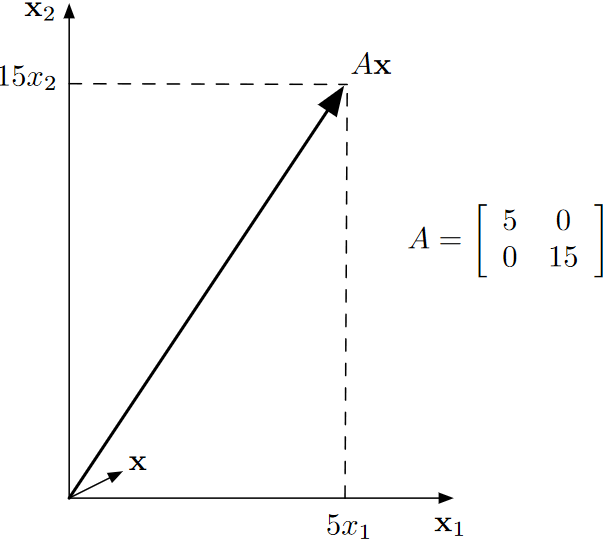
\includegraphics[width=0.5\textwidth]{
		images/04_LinearAlgebra_scalingVector.png
	}
	\caption{Scaling transformation in standard basis.}
	\label{fig:scalar_trans}
\end{figure}

\subsection{Scaling transformation in eigenbasis}
Consider Figure \ref{fig:eigenbasis_trans}.
\begin{itemize}
	\item Let $A$ be a non-scaling linear transformation in $\mathcal{R}^{2}$.
		Actually, transformation $Av$ is not a linear transformation, since $v$ has
		no components along the x\-axis.

	\item Let $\{v_{1}, v_{2}\}$ be an \textit{eigenbasis} for $A$. An eigenbasis is
		a basis in which every vector is an eigenvector.

	\item By representing vectors in $\mathcal{R}^{2}$ in terms of the $\{v_{1},v_{2}
		\}$ basis (instead of the standard $\{x_{1}, x_{2}\}$), $A$ becomes a
		scaling transformation.
\end{itemize}

Eigendecomposition is useful since we can compute an eigenbasis for a matrix $A$
so that $A$ becomes a scaling transformation with respect to the coordinate
system defined by the eigenbasis.

\begin{figure}[H]
	\centering
	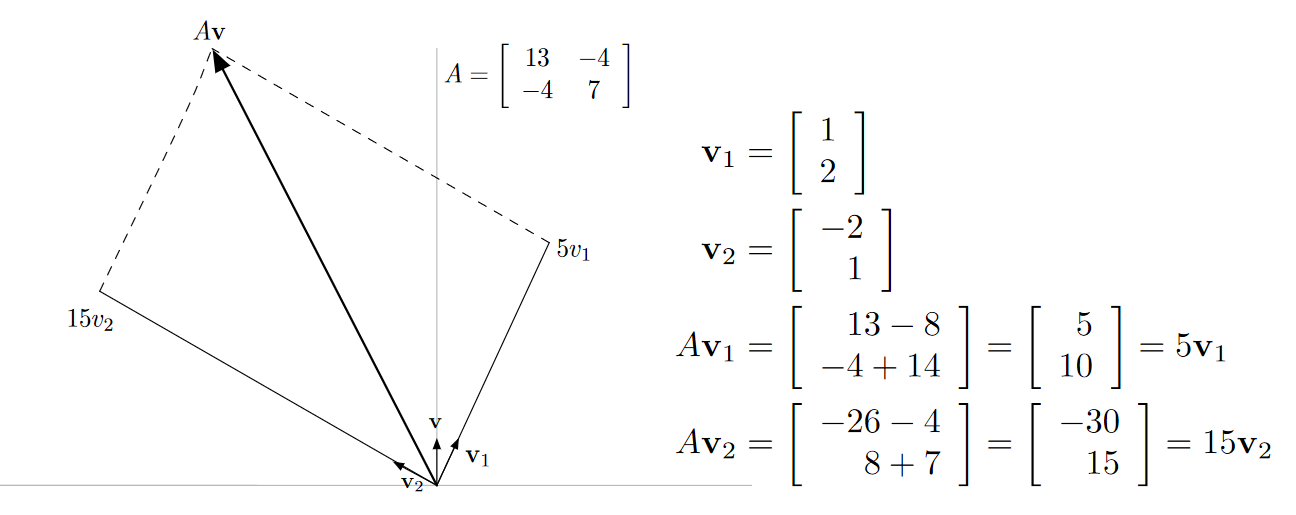
\includegraphics[width=\textwidth]{
		images/04_LinearAlgebra_eigenbasisTransformation.png
	}
	\caption{Scaling transformation in eigenbasis.}
	\label{fig:eigenbasis_trans}
\end{figure}

\section{Principal Component Analysis (PCA)}
Consider Figure \ref{fig:eigen_PCA}. $X$,$Y$ could be the height and the weight
of a person. These two dimensions are correlated. As a result, if we collect some
data from a population, we would obtain a distribution similar to the one
represented on the left side of Figure \ref{fig:eigen_PCA}. On the other hand,
the graphic on the right of Figure \ref{fig:eigen_PCA}, represents two quantities
$P1, P2$ which are apparently uncorrelated. Indeed, the data spreads along the two
dimensions.

\begin{itemize}
	\item Let $A$ be a data matrix with correlated coordinates.

	\item PCA is a linear transformation mapping data to a system of uncorrelated coordinates.

	\item It corresponds to fitting an ellipsoid to the data, whose axes are the
		coordinates of the new space.
\end{itemize}

\begin{figure}[H]
	\centering
	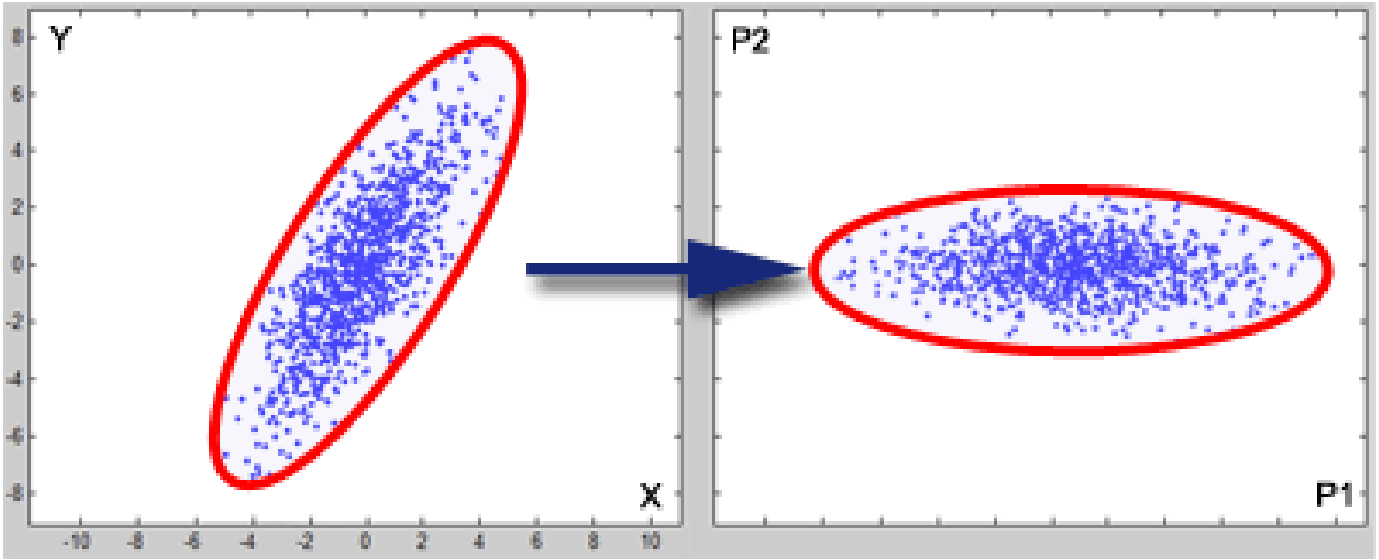
\includegraphics[width=\textwidth]{images/04_LinearAlgebra_PCA.png}
	\caption{Principal Component Analysis (PCA).}
	\label{fig:eigen_PCA}
\end{figure}

Given a dataset $X \in \mathcal{R}^{n \times d}$ with $n$ examples and $d$ dimensions.

\begin{enumerate}
	\item Compute the mean of the data ($X_{i}$ is the $i^{th}$ row vector of $X$):
		\begin{equation*}
			\Bar{x}= \frac{1}{n}\sum_{i=1}^{n}X_{i}
		\end{equation*}

	\item Center the data into the origin:
		\begin{equation*}
			X = X -
			\begin{bmatrix}
				\Bar{x} \\
				\vdots  \\
				\Bar{x}
			\end{bmatrix}
		\end{equation*}

	\item Compute the data covariance:
		\begin{equation*}
			C = \frac{1}{n}X^{T}X
		\end{equation*}
		The covariance information highlights the correlations between the
		dimensions.

	\item Compute the (orthonormal) eigendecomposition of $C$:
		\begin{equation*}
			V^{T}C V = \Lambda
		\end{equation*}

	\item Use the set of eigen vectors as the new coordinate system:
		\begin{equation*}
			x' = V^{-1}x = V^{T}x
		\end{equation*}
		($V^{-1}= V^{T}$ as $V$ is unitary). In this new space (represented by the
		axis of the ellipse) the data are uncorrelated.
\end{enumerate}

\textbf{Remark:} this procedure assumes linear correlations (and Gaussian
distributions).

\subsection{Dimensionality reduction}
Assume that we have computed the covariance matrix $C$ of a certain data distribution.
What is more, we have also performed eigen value - eigen vector decomposition.
At this point, it is possible to proof that each eigenvalue corresponds to the amount
of variance in the direction of the corresponding eigenvector. The eigen vector
which corresponds to the largest eigen values represents the directions of
largest spread. The dimensions with the largest spread are the dimensions with the
largest information. In order to perform \textit{dimensionality reduction} (e.g.
visualization), we select only the $k$ eigenvectors with largest eigenvalues.\\ Suppose
that we want to map the data in a $d$ dimensional space in a lower dimensional space
with $k$ dimensions. To do this, we execute the same procedure described above for
PCA, but this time we take into consideration only the first $k$ eigenvectors of
the covariance matrix decomposition.
\begin{equation*}
	W = [v_{1}, \hdots, v_{k}]
\end{equation*}
Then, it is straightforward to map a point in the primary space to the new lower
$k$-dimensional space (which retains the most information in terms of linear correlations):
\begin{equation*}
	x' = W^{T}x
\end{equation*}

Dimensionality reduction could be a valid pre-computation before applying other
machine learning algorithms which perhaps performs poorly on high dimensional
scenarios.
    \chapter{Probability theory}
\label{cha:probability}

\section{Discrete random variables}
    A discrete variable can assume a value in a range of possible values, it can not get values in between. 
    
    \defi{\textbf{Probability mass function}: \label{defi_prob_mass_funct}\\
    Given a discrete random variable $X$ taking values in $\mathcal{X} = \{v_1, ..., v_n\}$, its probability mass function $P: \mathcal{X} \rightarrow [0, 1]$ is defined as:
    $$P(V_i) = Pr(X=v_i)$$
    and satisfies the following conditions:
    \begin{itemize}
        \item $P(x) \geq 0$
        \item $\sum_{x \in \mathcal{X}}{P(x)} = 1$
    \end{itemize}
    }
    
    \defi{\textbf{Expected value}: \label{def:expected_value}\\
    The expected value (mean or average) of a random variable is:
    $$E[X] = \mu = \sum_{x \in \mathcal{X}} xP(x) = \sum_{i=1}^{m}v_{i}P(v_{i})$$
    This is a linear operator, that implies:
    $$E[\lambda x +\lambda ' y] = \lambda E[y] + \lambda ' E[y]$$
    }
    
    \defi{\textbf{Variance}: \label{def:variance}\\
    The variance of a random variable is the moment of inertia of its probability mass function:
    $$Var[x] = \sigma ^2 = E[(x - \mu)^2] = \sum_{x \in \mathcal{X}}(x - \mu)^2 P(x)$$
    The standard deviation $\sigma$ indicates the typical amount of deviation from the mean one should expect for a randomly drawn value of x.
    }
    
    Variance is \textbf{not} a linear operator.
    Therefore:\\
    $$Var[x] = E[x^2] = E[x]^2$$
    $$Var[\lambda x] = \lambda ^2 Var[X]$$
    And for \textbf{uncorrelated variables} $x, y$ it is true that\\
    $$Var[x+y] = Var[x] + Var[y]$$
    
    \subsection{Probability distributions for discrete variables}
        
        \defi{\textbf{Bernoulli distribution}: \label{defi:bernoullo_dist}\\
        The Bernoulli distribution applies on variables that can assume binary outcomes (0/1, true/false, success/failure). Being $p$ the parameter of success, its probability mass function is defines as:
        $$P(x;p) = 
            \begin{cases} 
            p & if\ x = 1\\ 
            1-p &if\ x = 0
            \end{cases}
        $$
        The expected value for a Bernoulli distribution is $p$ and the variance is equal to $p(1-p)$.
        }
        
        \defi{\textbf{Binomial distribution}: \label{def:binomial_dist}\\
        The binomial distribution is a Bernoulli distribution extended to a certain number $n$ of trials. Its probability mass function is:
        $$P(x;p,n) = \binom{n}{x}p^x(1-p)^{n-x}$$
        The expected value for a Binomial distribution is $np$ and the variance is equal to $np(1-p)$.
        }
        
        It is easy to see that a Bernoulli distribution is per se a Binomial distribution in the trivial case where $n=1$.\\
        A Bernoulli distribution can be used for modelling the toss of a coin, whereas the Binomial distribution describes the event of the coin has been tossed $n$ times.
        
        \defi{\textbf{Multinomial distribution}\label{def:mutltinomial_dist}\\
        The multinomial distribution models the probability of an event that can have $m$ different outcomes, each with (possibly) a different probability. Its probability mass function is:
        $$P(x_1, \dots, x_m; p_1, \dots p_m) =  \prod_{i=1}^m p_i^{x_i}$$
        where
        \begin{itemize}
            \item $x_1, \dots, x_m$ is a vector that represents the outcome,
            \item $E[x_i] = p_i$
            \item $Var[x_i] = p_i(1-p_i)$
            \item $Cov[x_i, x_j] = -p_i p_j$
        \end{itemize}
        }
        
        Examples of outcome vectors for a 6-faces dice (d6) are:
        $$x_1 = [1, 0, 0, 0, 0, 0],$$
        $$x_2 = [0, 1, 0, 0, 0, 0],$$
        $$x_3 = [0, 0, 1, 0, 0, 0],$$
        $$x_4 = [0, 0, 0, 1, 0, 0],$$
        $$x_5 = [0, 0, 0, 0, 1, 0],$$ 
        $$x_6 = [0, 0, 0, 0, 0, 1]$$
        in which the first column represents the success of the event of getting one as result, the second column the event of getting two and so on so forth. Since the event are mutually exclusive, just one column is signed as $1$.
        For a fair dice, the vector or probabilities would be:
        $$p =  \left[ \frac{1}{6}, \frac{1}{6}, \frac{1}{6}, \frac{1}{6}, \frac{1}{6}, \frac{1}{6} \right] $$
        
        \defi{\textbf{Multinomial distribution (general case)}\\
        Given $n$ repetition of an event which can end uo in $m$ possible outcome, $p=\{p_1, \dots, p_m\}$ the probability of each of the outcomes, the probability mass function is
        $$P(x_1, \dots, x_m; p_1, \dots, p_m, n) = \dfrac{n!}{\prod\limits_{i=1}^mx_i!}\prod\limits_{i=1}^mp_i^{x_i}$$
        In this distribution $E[x_i] = np_i$, $Var[x_i] = np_i(1-p_i)$ and $Cov[x_i, x_j] = -np_i p_j$
        }
        Also this last case is a generalization of every case described above, but four our purposes will not be used, it is reported for completeness.
        
    \subsection{Pairs of discrete random variables}
        
        \defi{\textbf{Joint probability mass function}: \label{def:joint_prob_mass_funct}\\
        Given a pair of discrete random variables $X, Y$ taking values $\mathcal{X} = \{v_1, ..., v_n\}$ and $\mathcal{Y} = \{y_1, ..., y_n\}$, the joint probability mass function is defined as:
        $$P(v_i, w_j) = Pr[X = v_i, Y = w_j]$$
        This function has the following properties:
        \begin{itemize}
            \item $P(x, y) \geq 0$
            \item $\sum_{x \in \mathcal{X}} \sum_{y \in \mathcal{Y}} P(x, y) = 1$
        \end{itemize}
        }
        
        Its expected values are:
        $$\mu_{x} = E[x] = x\sum_{x \in \mathcal{X}} \sum_{y \in \mathcal{Y}} P(x, y)$$
        $$\mu_{y} = E[y] = y\sum_{x \in \mathcal{X}} \sum_{y \in \mathcal{Y}} P(x, y)$$
        The variances are:
        $$\sigma_{x}^2 = Var[(x - \mu_{x})^2] = \sum_{x \in \mathcal{X}} \sum_{y \in \mathcal{Y}} (x - \mu_{x})^2 P(x, y)$$
        $$\sigma_{y}^2 = Var[(y - \mu_{y})^2] = \sum_{x \in \mathcal{X}} \sum_{y \in \mathcal{Y}} (y - \mu_{y})^2P(x, y)$$
        The covariance (expectation of how much they can co-vary) is:
        $$\sigma_{xy} = E[(x-\mu_{x})(y-\mu_{y})] = \sum_{x\in \mathcal{X}} \sum_{y \in \mathcal{Y}} (x-\mu_{x}) (y - \mu_{y}) P(x, y)$$
        From these values we can get a coefficient of correlation as:
        $$\rho = \frac{\sigma_{xy}}{\sigma{x}\sigma{y}}$$
        This measure is the ratio between the covariance of two variables and the product of their standard deviations; thus, it is essentially a normalized measurement of the covariance, such that the result always has a value between -1 and 1.
        
\section{Conditional probabilities}
    If two variables are not independent, we can apply some laws and rules to get their probability and conditional probabilities.
    
    \theo{\textbf{Law of total probability}\\
    The marginal distribution of a variable is obtained from a joint distribution summing over all possible values of the other variable.
    
    $$P(x) = \sum_{y \in \mathcal{Y}} P(x, y)$$ 
    and
    $$P(y) = \sum_{x \in \mathcal{X}} P(x, y)$$ 
    }
    
    \theo{\textbf{Produt rule, Bayes' rule}\label{theo:bayes}\\
    Given two variables $x, y$ we can get the conditional probability from Bayes' rule as:
    $$P(x|y)P(y) = p(y|x)P(x)$$
    }
    
    This is important because it allows to get information about a posterior probability given the initial conditions and the likelyhood of the linkage.
    
    $$posterior = \frac{likelyhood \times prior}{evidence}$$
    
    Prior and evidence are the data related to the single variables and likelyhood is the effect produced by the cause.\\
    These rules apply also to more than two variables:
    $$P(y) = \sum_x \sum_z P(x, y, z)$$
    $$P(y) = \sum_x \sum_z P(y | x, z) P(x, z)$$
    also for conditional probability:
    $$P(y) = \sum_x \sum_y \frac{P(x|y, x)P(y|z)P(x, z)}{P(x|z)}$$
    Overall it is true that:
    $$P(y|x, z) = \frac{P(x|z, y)P(y|z)}{P(x|z)}$$
    
\section{Continuous random variables}
    Continuous variables allows us to assign non-discrete values, for example the height of a range of people, what we do is assigning intervals. 
    The probability mass function can be generalized on continuous domains.\\
    Given $W = (a < X \leq b)$ then $A = (X \leq a)$ and $B = (X \leq b)$. W and A end up to be mutually exclusive, so 
    $$P(B) = P(A) + P(W)$$
    
    \defi{\textbf{Cumulative distribution}\label{def:cumulative_dist}\\
    Given a continuous variable $X$ we define 
    $$F(q) = P(X \leq q)$$
    the cumulative distribution of X. 
    F is a monotonic function.\\
    Given and interval $a < X \leq b$, the probability of $X$ is described as the difference of the edge values:
    $$P(a < X \leq b) = F(b) - F(a)$$
    }
    
    \defi{\textbf{Probability density function}\label{def:prob_density_func}\\
    The derivative of the cumulative distribution is called density function.
    $$p(x) = \frac{d}{dx}F(x)$$
    This corresponds to the mass function for continuous values. Therefore is true that
    $$F(q) = P(X \leq q) = \int_{-\infty}^q p(x)dx $$
    The probability density function has these properties:
    \begin{itemize}
        \item $p(x) \geq 0$
        \item $\int_{-\infty}^{\infty} p(x)dx = 1$ which stands for the sum of all possible cases.
    \end{itemize}
    }
    
    Also mean and variance \ref{def:expected_value} \ref{def:variance} are computed in the same way, but taking into account the infinite number of small interval, therefore computing an integral as well.
    
    $$E[x] = \mu = \int_{-\infty}^{\infty} xp(x)dx$$
    $$Var[x] = \sigma ^2 = \int_{-\infty}^{\infty} (x-\mu)^2 p(x)dx$$
    
    \subsection{Probability distributions for continuous variables}
        \defi{\textbf{Gaussian or Normal distribution ($\mathcal{N}$)}\label{def:gaussian_normal}\\
        The Gaussian distribution is a bell-shaped function that is the standard for fitting continuous data. The mean is the highest point in the graph while the variance is the spreading of the data from the mean.\\
        The probability density function is
        $$p(x; \mu, \sigma) = \frac{1}{\sqrt{2\pi}\sigma} \exp^{-\frac{(x-\mu)^2}{2\sigma ^2}}$$
        A standard distribution is denoted as $\mathcal{N}(0, 1)$ where $\mu = 0$ and $\sigma = 1$, \\
        whereas a standardization of a normal distribution is $\mathcal{N}(\mu, \sigma^2)$, it is carried on through this formula:
        $$z = \frac{x-\mu}{\sigma}$$
        }
        
        \begin{figure}
            \centering
            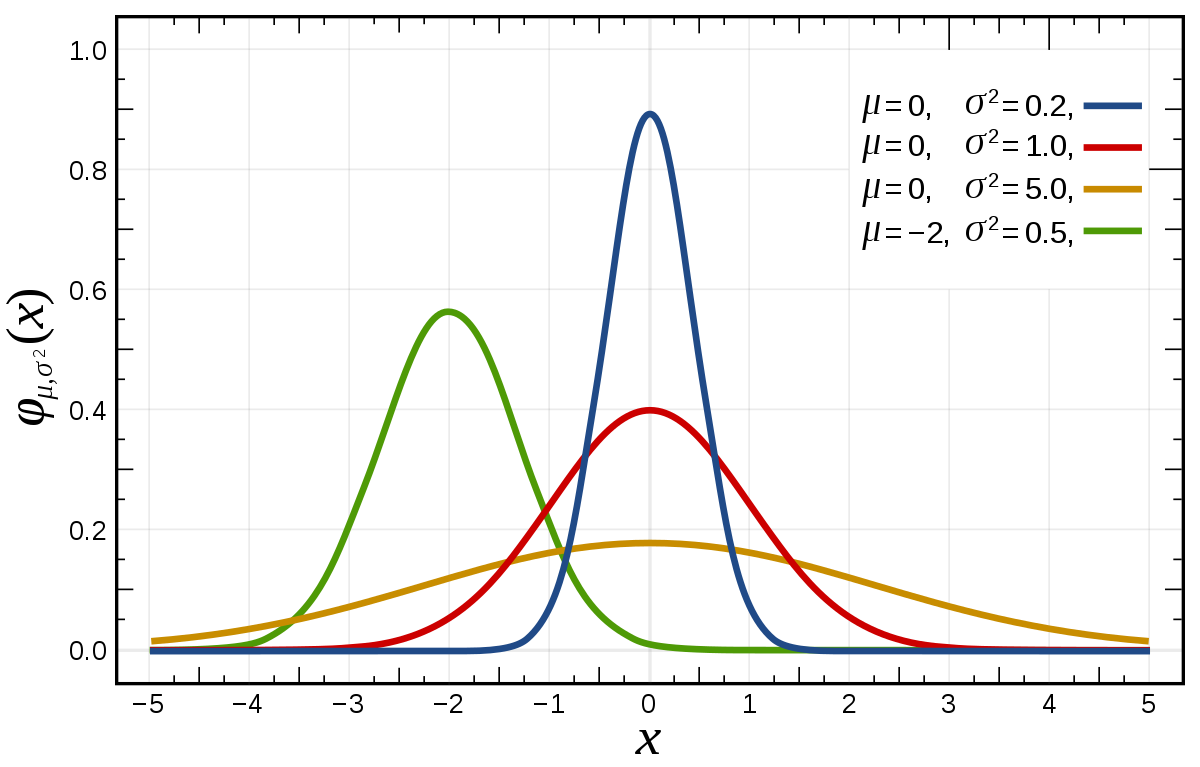
\includegraphics[scale=0.2]{images/gaussian.png}
            \caption{Set of Gaussian distributions}
            \label{fig:Gaussian_1}
        \end{figure}
        
        \defi{\textbf{Beta distribution}\label{def:beta_dist}\\
        The beta distribution is a second degree order of probability distribution (as the probability of a probability) that is defined in the interval $[0, 1]$ with parameters $\alpha$ and $\beta$. Its probability density function is
        $$p(x;\alpha, \beta) = \frac{\Gamma(\alpha + \beta)}{\Gamma(\alpha)\Gamma(\beta)}x^{\alpha-1}(1-x)^{\beta-1}$$
        where
        \begin{itemize}
			\item $\mathbb{E}[x] = \frac{\alpha}{\alpha+\beta}$
			\item $Var[x] = \frac{\alpha\beta}{(\alpha+\beta)^2(\alpha+\beta+1)}$
			\item $\Gamma(x+1) = x\Gamma(x)$
			\item $\Gamma(1) = 1$
		\end{itemize}
        }
        This distribution focuses on describing the distribution of a parameter $p$ of a binomial distribution after observing $\alpha -1$ independent events with probability $p$ and $\beta -1$ with probability $1-p$.
        
        \defi{\textbf{Multivariate normal distribution}\label{def:multi_normal_dist}\\
        This distribution aims to define a Gaussian distribution extended to $d$ dimensions. In order to define such distribution we need a mean $\mu$ and $\Sigma$ covariance matrix.
        Its probability density function is described as
        $$p(\vec{x}, \vec{\mu}, \Sigma) = \frac{1}{(2\pi)^{\frac{d}{2}}|\Sigma|^{\frac{1}{2}}}e^{-\frac{1}{2}(\vec{x}-\vec{\mu})^T\Sigma^{-1}(\vec{x}-\vec{\mu})}$$
        Relevant features are:
        \begin{itemize}
            \item $E[x] = \mu$
            \item $Var[x] = \Sigma$
            \item the squared Mahalanobis distance from x to $\mu$ is \\$r^2 = (x-\mu)^T \Sigma ^{-1} (x-\mu)$
        \end{itemize}
        }
        
        \begin{figure}
            \centering
            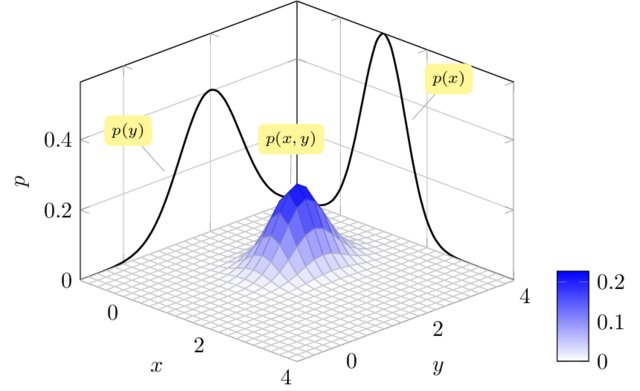
\includegraphics[scale=1]{images/multivariate_distribution.jpg}
            \caption{Multivariate normal distribution for $d=3$}
            \label{fig:Gaussian_2}
        \end{figure}
        
        \defi{\textbf{Dirichlet distribution}\label{def:diri_dist}\\
        This distribution is defined for $x \in [0, 1]^m$, $\sum_{i=1}^m x_i = 1$, the parameters it is based on are $\alpha = \alpha_1, \dots, \alpha_m$ and its probability density function is
        $$p(x_1, \dots, x_m; \vec{\alpha}) = \frac{\Gamma(\alpha_0)}{\prod\limits_{i=1}^m\Gamma(\alpha_i)}\prod\limits_{i=1}^mx_i^{a_i-1}$$
		Where $\alpha_0 = \sum_{j=1}^m \alpha_j$.
		
		Characterizing values of this distribution are:
		\begin{itemize}
		    \item $E[x_i] = \frac{\alpha_1}{\alpha_0}$
		    \item $Var[x_i] = \frac{\alpha_i(\alpha_0-\alpha_i)}{\alpha_0^2(\alpha_0+1)}$
		    \item $Cov[x_i, x_j] = \frac{-\alpha_i\alpha_j}{a_0^2(\alpha_0+1)}$
		\end{itemize}
		
		This distribution can model a posterior distribution of parameters $p$ of a multinomial distribution after observing $\alpha_i -1$ times each mutually exclusive events.
        }

\section{Probability laws}
    Let's consider a sample of $X_1, \dots, X_n$ \textbf{independent} instances from a distribution with mean $\mu$ and variance $\sigma^2$. 
    We can get a \textbf{mean of the obervated values} as
    $$\bar{X}_n = \frac{X_1 + \dots + X_n}{n}$$
    and his expectation will be equals to $\mu$
    $$E[\bar{X}_n] = \mu$$
    Its variance (iff they are \textbf{independent}) will be computed as 
    $$Var[a(X+Y)] = a^2(Var[X] + Var[Y])$$
    and the mean of the computed variance will be
    $$Var[\bar{X}_n] = \frac{1}{n^2}(Var[X_1] + \cdots Var[X_n]) = \frac{\sigma^2}{n}$$
    that means that the variance of the average decreases as the number of observation increases (the higher the number of the observation, the higher the precision of the estimate).
    
    \theo{\textbf{Chebyshev's inequality}\label{theo:Chebyshev}\\
    Given a random variable $X$ with mean $\mu$ and variance $\sigma^2$, for all $a > 0$
    $$Pr[|X-\mu| \geq a] \leq \frac{\sigma^2}{a^2}$$
    this implies the more $X$ differs from the mean more than $a$ the more $\sigma^2$ gets bigger and vice versa.\\
    Also, replacing $a = k\sigma$ for $k>0$
    $$Pr[|X - \mu| \geq k\sigma] \leq \frac{1}{k^2}$$
    This inequality shows that most of the probability mass of a random variable stays within few standard deviations from its mean.
    }
    
    \theo{\textbf{Law of large numbers}\label{theo:large_numbers}\\
    Considering a sample of $X_1, \dots, X_n$ independent instances from a distribution with mean $\mu$ and variance $\sigma^2$,
    for any $\epsilon > 0$ it is true that the object $\bar{X_n}$ obeys:
    $$\lim_{n \rightarrow \infty} Pr[|\bar{X_n}| > \epsilon] = 0$$
    Using Chebyschev's inequality and knowing that
    $E[\bar{X_n}] = \mu$ and also $Var[\bar{X_n}] = \frac{\sigma^2}{n}$ it comes that 
    $$Pr[|\bar{X_n} - E[\bar{X_n}]| > \epsilon] \leq \frac{\sigma^2}{n\epsilon^2}$$
    
    }
    
    Overall this means that increasing the number of observation of a certain events allows us to get closer to the actual mean $\mu$ so the accuracy increases. Also this means that the variance gets closer (less uncertainty, relatively less values far away from the actual mean).
    
    \theo{\textbf{Central limit theorem}\label{theo:central_limit}\\
    Considering a sample $X_1, \dots, X_n$ of idipendent instances drawn from a distribution with mean $\mu$ and variance $\sigma^2$, then
    \begin{enumerate}
        \item regardless the distribution of $X_i$, for $n \rightarrow \infty$ the distribution of the sample average $\bar{X_n}$ approaches to a Normal distribution $\mathcal{N}$
        \item Its mean approaches to $\mu$ and its variance approaches to $\frac{\sigma^2}{n}$
        \item Thus the normalized sample average:
        $$z = \frac{\bar{X_n} - \mu}{\cfrac{\sigma}{\sqrt{n}}}$$
        approaches to a normal distribution $\mathcal{N} (0, 1)$ 
    \end{enumerate}
    }
    
    The Central Limit theorem implies that:
    \begin{itemize}
        \item the sum of a sufficiently large sample of independent random measurements is \textbf{approximately normally distributed}
        \item there is \textbf{no need to know the actual distribution}
        \item justifies the \textbf{importance of the Gaussian} distribution in the real world applications
    \end{itemize}
    
    \section{Information theory}
        Consider a discrete set of symbols $\mathcal{V} = \{v_1, \dots, v_n\}$ with mutually exclusive probabilities $P(V_i)$.
        We aim designing a binary codification for each symbol that minimize the overall length of messages encoded in binary.
        This optimal code assign to each symbol $v_i$ a number of bits equals to $- \log P(v_i)$.\\
        
        \defi{\textbf{Entropy}\label{def:entropy_probability}\\
        The entropy of the set of symbols is the expected length of a message encoding a symbol assuming each such optimal coding
        $$H[\mathcal{V}] = E[-\log P(v)] = -\sum_{i=1}^n P(v_i) \log P(v_i)$$
        
        }
        
        \defi{\textbf{Cross entropy}\label{def:cross_entropy}\\
        Considering two distributions $P$ and $Q$ over a variable $X$, the cross entropy between the two distributions measures the expected number of bits needed to code a symbol sampled from P using Q instead:
        $$H(P;Q) = \mathbb{E}_P[-\log Q(v)] = -\sum_{i=1}^n P(v_i)\log Q(v_i)$$
        
        }
        
        This is also used as a loss in binary classification (with $P$ as empirical true distribution and $Q$ ad empirical predicted distribution).
        
        From these two definition we get the concept of \textbf{relative entropy}.
        
        \defi{\textbf{Relative entropy}\label{def:relative_entropy}\\
        Consider two distribution $P$ and $Q$ over a variable $X$, the relative entropy divergence (KL) measures the expected length difference when coding instances samples from $P$ using $Q$ instead:
        $$D_{KL} (p||q) = H(P; Q) - H(P)$$
        %$$D_{KL} (p||q) = -\sum_{i=1}^n P(v_i)\log Q(v_i) +\sum_{i=1}^n \log P(v_i)$$
        therefore
        $$D_{KL} (p||q) = \sum_{i=1}^n P(v_i) \log \frac{P(v_i)}{Q(v_i)}$$
        }
        
        \defi{\textbf{Conditional entropy}\label{def:conditional_entropy}\\
        Consider two variables $V, W$ with (possibly different) distribution $P$, then the conditional entropy of the entropy remaining for variable $W$ once $V$ is known:
        $$H(W|V) = \sum_v P(v)H(W|V=v)$$
		$$H(W|V) =\sum_{v} P(v)\sum_w P(w|v)\log P(w|v)$$
        }
        
        The conditional entropy allows to get insight of the information gain (reduction of entropy for $W$).
        
        \defi{\textbf{Mutual information}\label{def:mutual_info}\\
        Given two variables $V, W$ with (possibly different) distribution $P$. The mutual information (or \textit{information gain}) is the reduction in entropy for $W$ once $V$ is known:
        $$I(W; V) = H(W) - H(W|V)$$
        $$I(W; V) = -\sum_{w} P(w)\log P(w) + \sum_{v} P(v)\sum_w P(w|v)\log P(w|v)$$
        }   
        
        Concept as the entropy are used to build ML models, as a decision trees \ref{cha:decision_trees}: this value is indeed taken into account when we are trying to select the most clever feature on which the separation in the subset will be based on. 
    \chapter{Evaluation}
\label{cha:evaluation} Evaluation requires to define performance measures to be optimized.
The evaluation process differs from solving a classic optimization problem. Indeed,
performance of learning algorithms cannot be evaluated on entire domain. The purpose
of machine learning is to learn a model from a restricted training set and perform
generalization from this knowledge. Performance evaluation is needed for:
\begin{itemize}
	\item tuning hyperparameters of learning methods (e.g. type of kernel and kernel
		parameters, learning rate of perceptron)

	\item evaluating quality of learned predictor

	\item computing statistical significance of difference between learning algorithms
\end{itemize}

The training loss function measures the cost paid for predicting $f(x)$ for
output $y$ ($f(x)$ is the predicted value; $y$ is the ground truth). It is
designed to boost effectiveness and efficiency of learning algorithms (e.g.
\textit{hinge loss} for SVM). Typically the purpose of the training is to minimize
a training loss. As a consequence, ideal training loss functions are smooth,
differentiable. As a result, not all the performance measures can be used as
loss functions. Actually there is a difference between a loss function and the final
performance measure. For example, \textit{accuracy} (i.e. fraction of examples
correctly classified) is a performance measure which can not be used as a loss function.
More in depth, accuracy (or misclassification cost) is never used as a loss function,
since it is \textit{piecewise constant} and so not amenable to gradient descent.
A function is said to be piecewise constant if it is locally constant in
connected regions separated by a possibly infinite number of lower-dimensional
boundaries. Square wave (Figure \ref{fig:square_wave}) is an example of piecewise
constant function. This latter is not differentiable in correspondence of the
jumps and has first derivative equals to zero when it is constant. The gradient cannot
be computed or it is zero and so it does not indicate where to move in order to find
the optimum.

\begin{figure}[H]
	\centering
	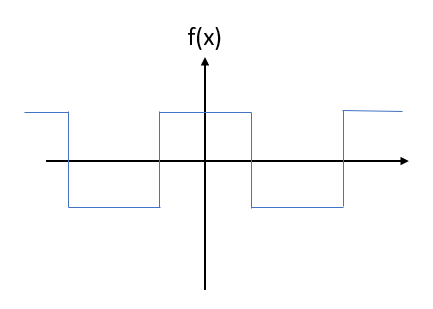
\includegraphics[width=0.5\textwidth]{
		images/06_Evaluation_squareWaveFunction.png
	}
	\caption{Square wave function is an example of piecewise constant function.}
	\label{fig:square_wave}
\end{figure}

An example of training loss function is \textit{cross entropy loss}.
\newline

Typically it is useful to consider multiple performance measures which can highlight
complementary information about the model under study.

\section{Binary classification}
\label{sec::performanceBinaryClassification} The typical way to visualize the performance
of a classification algorithm is by means of a \textit{confusion matrix}. This last
is a table which has the possible labels as rows and columns. In particular, the
rows represent the true labels for the data, while the columns report the
predicted labels. In the case of binary classification, the confusion matrix can
be exemplified as illustrated in Figure \ref{fig:binClassConfusionMatrix}.

\begin{itemize}
	\item TP $\rightarrow$ true positives: positives predicted as positives

	\item TN $\rightarrow$ true negatives: negatives predicted as negatives

	\item FP $\rightarrow$ false positives: negatives predicted as positives

	\item FN $\rightarrow$ false negatives: positives predicted as negatives
\end{itemize}

\begin{table}[ht]
	\centering
	\begin{tabular}{cc|cc|}
		\cline{3-4}                                         &   & \multicolumn{2}{c|}{prediction} \\
		\cline{3-4}                                         &   & \multicolumn{1}{c|}{P}         & N  \\
		\hline
		\multicolumn{1}{|c|}{\multirow{2}{*}{ground truth}} & P & \multicolumn{1}{c|}{TP}        & FN \\
		\cline{2-4} \multicolumn{1}{|c|}{}                  & N & \multicolumn{1}{c|}{FP}        & TN \\
		\hline
	\end{tabular}
	\caption{Confusion matrix for binary classification}
	\label{fig:binClassConfusionMatrix}
\end{table}

From the confusion matrix it is possible to compute several performance measures.

\defi{\textbf{Accuracy} \label{def:accuracy}\\ \textit{Accuracy} is the fraction of correctly labelled examples among all predictions. \begin{equation}\mathit{Acc}= \frac{\mathit{TP}+\mathit{TN}}{\mathit{TP}+\mathit{TN}+\mathit{FP}+\mathit{FN}}\end{equation}

\textbf{Remark:} accuracy is one minus the misclassification cost. }

Accuracy is not informative for strongly unbalanced datasets (typically negatives
much more than positives). For instance, if we monitor the presence of a rare
pathology in a set of people, negatives example would be much more than positives.
In this context, predictions are dominated by the larger class. As a consequence,
predicting everything as negative often maximizes the accuracy without learning nothing.
A possible solution consists of \textit{rebalancing} costs. Following this
technique, a positive example does not count as one but it counts as $\frac{N}{P}$
where $N=TN+FP$ and $P=TP+FN$. In this way, if we have 10 times more negatives,
when the model predicts a positive correctly, it does not count as one point but
it counts as 10 points.

\defi{\textbf{Precision} \label{def:precision}\\ \textit{Precision} is the fraction of positives among examples predicted as positives. \begin{equation}\mathit{Pre}= \frac{\mathit{TP}}{\mathit{TP}+\mathit{FP}}\end{equation}

It measures the precision of the learner when predicting positive. }

\textbf{Remark:} a problem of this measure is that I can improve precision by
predicting positive very rarely. For this reason a the following complementary measure
is introduced.

\defi{\textbf{Recall or Sensitivity} \label{def:recall}\\ \textit{Recall} (or \textit{sensitivity}) is the fraction of positive examples predicted as positives. \begin{equation}\mathit{Rec}= \frac{\mathit{TP}}{\mathit{TP}+\mathit{FN}}\end{equation} It measures the coverage of the learner in returning positive examples. }
Since these last two measures are complementary, i.e. when precision increases, the
recall typically decreases, it is not usually appropriate to consider them
separately. Nevertheless, in some contexts it could be reasonable to consider
recall and precision separately. Consider an in information retrieval task like:
"\textit{Give me the pages about machine learning from DISI website}". In this
case it is crucial to achieve a good precision in the first results of the
searching algorithm output. Vice versa, if we aim to develop a cancer detection
application, recall has to be prioritized.\\ For standard classification tasks,
there is a measure which combines recall and precision balancing the two aspects.

\defi{\textbf{F-measure} \label{def:fmeasure}\\ \textit{F-measure} combines precision and recall balancing the two aspects. $\beta$ is a parameter trading\-off precision and recall. \begin{equation}\mathit{F_\beta}= \frac{(1+\beta^{2})(\mathit{Pre}\cdot \mathit{Rec})}{\beta^{2}\mathit{Pre}+ \mathit{Rec}}\end{equation} }

The most common version of F-measure is the $F_{1}$-measure which sets $\beta=1$.
$F_{1}$ is the \textit{harmonic mean} of precision and recall. A good trade off between
precision and recall is needed in order to have a high value of $F_{1}$. $F_{1}$
is a good performance measure (better then accuracy) in the case of unbalanced
datasets.
\begin{equation}
	F_{1}= \frac{2(\mathit{Pre} \cdot \mathit{Rec})}{\mathit{Pre} + \mathit{Rec}}
\end{equation}
Classifiers often provide a confidence in the prediction (e.g. random forests,
margin or SVM). In these cases it is possible to improve precision and/or recall
by moving the confidence threshold for deciding if an element has to be
classified positively or negatively. With a high threshold we would maximize precision.
On the other hand, low values of threshold tend to maximize recall. By varying
threshold from min to max possible value, we obtain a curve of performance measures.
This curve can be shown plotting one measure (recall) against the complementary
one (precision) (see Figure \ref{fig:precisionRecallCurve}).

\begin{figure}[H]
	\centering
	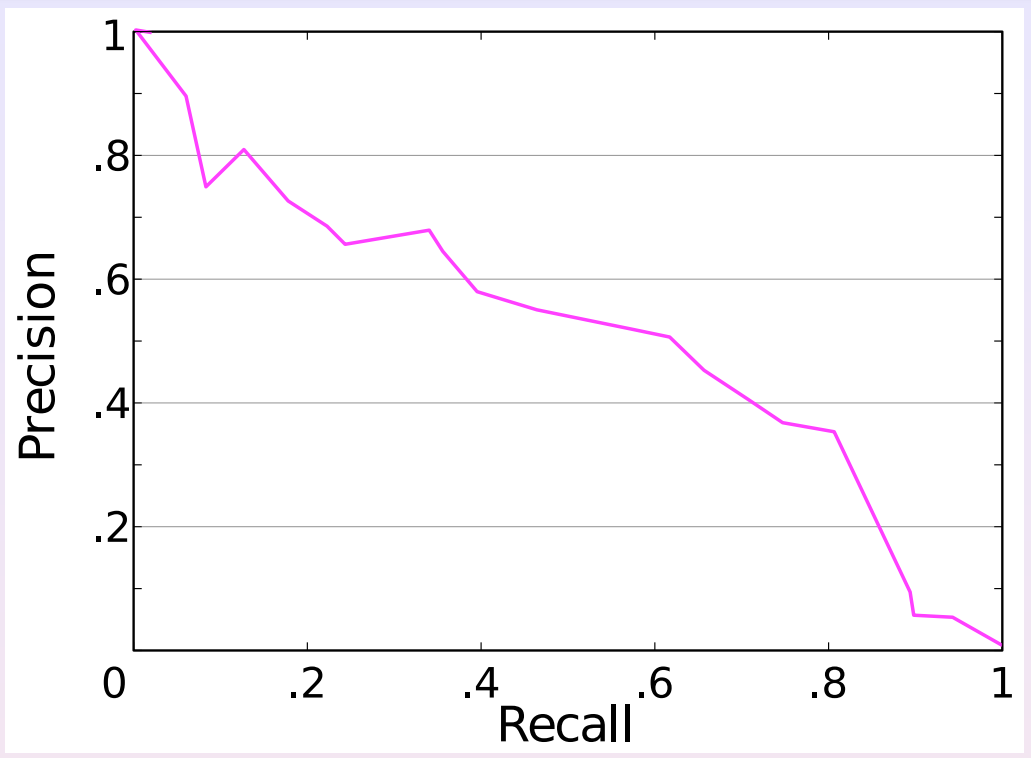
\includegraphics[width=0.5\textwidth]{
		images/06_Evaluation_precisionRecallCurve.png
	}
	\caption{Precision-recall curve. When the threshold is 0, we obtain very high
	precision, since in this case the model predicts positive only if it has very high
	confidence. On the right the graphic highlights high recall since the model
	predicts always positive with such a configuration.}
	\label{fig:precisionRecallCurve}
\end{figure}

With this tool, we can compare different algorithms by plotting them on the same
graphic. Then, we can decide the algorithm to use according to what we are
interested in.\\ A single aggregate value can be obtained taking the area under
the curve (see Figure \ref{fig:areaUnderPreRecCurve}). It combines the performance
of the algorithm for all possible thresholds (without preference for a specific
value of threshold). The area under the precision-recall curve is a good general
way to compare an algorithm with respect to another.

\begin{figure}[H]
	\centering
	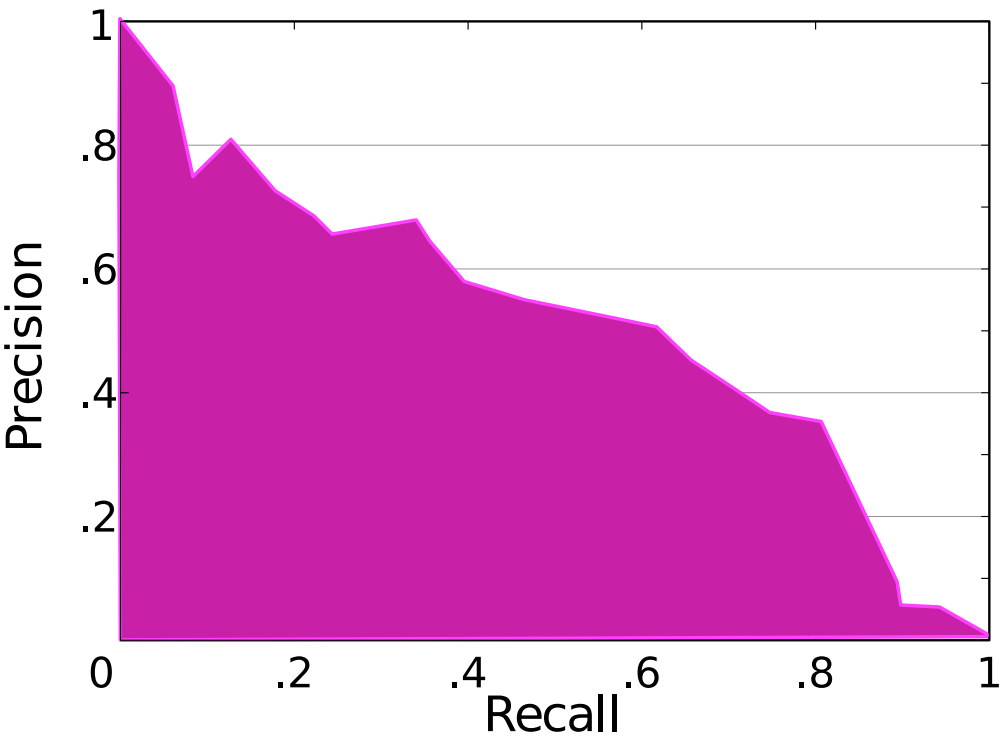
\includegraphics[width=0.5\textwidth]{
		images/06_Evaluation_areaPrecisionRecallCurve.png
	}
	\caption{Area under precision-recall curve.}
	\label{fig:areaUnderPreRecCurve}
\end{figure}

\section{Multiclass classification}
\label{sec::performanceMulticlassClassification} The notion introduced for binary
classification in Section \ref{sec::performanceBinaryClassification} can be extended
to the domain of multiclass classification.\\ The confusion matrix is a generalized
version of the binary one. The rows are the ground truth labels, while the columns
represents the predicted labels. The structure of a confusion matrix in the case
of multiclass classification is schematized in Figure
\ref{fig:confisionMatrixMulticlassClassification}.

\begin{table}[ht]
	\centering
	\begin{tabular}{cc|clc|}
		\cline{3-5}                                         &                              & \multicolumn{3}{c|}{prediction} \\
		\cline{3-5}                                         &                              & \multicolumn{1}{c|}{$y_{1}$}   & \multicolumn{1}{l|}{$y_{2}$}  & $y_{3}$                       \\
		\hline
		\multicolumn{1}{|c|}{\multirow{3}{*}{ground truth}} & $y_{1}$                      & \multicolumn{1}{c|}{$n_{11}$}  & \multicolumn{1}{l|}{$n_{12}$} & $n_{13}$                      \\
		\cline{2-5} \multicolumn{1}{|c|}{}                  & \multicolumn{1}{l|}{$y_{2}$} & \multicolumn{1}{l|}{$n_{21}$}  & \multicolumn{1}{l|}{$n_{22}$} & \multicolumn{1}{l|}{$n_{23}$} \\
		\cline{2-5} \multicolumn{1}{|c|}{}                  & $y_{3}$                      & \multicolumn{1}{c|}{$n_{31}$}  & \multicolumn{1}{l|}{$n_{32}$} & $n_{33}$                      \\
		\hline
	\end{tabular}
	\caption{Multiclass classification confusion matrix.}
	\label{fig:confisionMatrixMulticlassClassification}
\end{table}

\begin{itemize}
	\item $n_{ij}$ is the number of examples with class $y_{i}$ predicted as $y_{j}$

	\item the main diagonal contains true positives for each class

	\item the sum of off-diagonal elements along a column is the number of false positives
		for the column label:
		\[
			\mathit{FP}_{i}= \sum_{j \neq i}n_{ji}
		\]

	\item the sum of off-diagonal elements along a row is the number of false negatives
		for the row label:
		\[
			\mathit{FN}_{i}= \sum_{j \neq i}n_{ij}
		\]
\end{itemize}

At this point we can compute the performance measures discussed above in Section
\ref{sec::performanceBinaryClassification}. Accuracy, precision, recall, $F_{1}$-measure,
are defined "\textit{per-class}" (e.g. $\mathit{Pre}_{i}$ indicates the
precision of class $i$) considering as negatives examples from other classes.
\begin{itemize}
	\item Precision of class $i$
		\[
			\textit{Pre}_{i}= \frac{n_{ii}}{n_{ii}+\textit{FP}_{i}}
		\]

	\item Recall of class $i$
		\[
			\textit{Rec}_{i}= \frac{n_{ii}}{n_{ii}+\mathit{FN}_{i}}
		\]
\end{itemize}

An extension of the accuracy in a multiclass setting is the concept of \textit{multiclass
accuracy}.

\defi{\textbf{Multiclass accuracy} \label{def:multiclassAccuracy}\\ Multiclass accuracy is the overall fraction of correctly classified examples. \begin{equation}\mathit{MAcc}= \frac{\sum_{i}n_{ii}}{\sum_{i}\sum_{j}n_{ij}}\end{equation} }

In the same manner, we can compute $F_{1}$ for class $i$ and the average $F_{1}$
across classes.
\newline

From the confusion matrix we can infer the pair of classes which are often confused
by the classifier. This kind of observations could for example highlight the
need of considering additional features in order to disambiguate classes.

\section{Regression}
\textit{Root mean squared error} is the typical performance measure in the regression
domain. Intuitively, it represents the distance between the predicted value and the
real value.
\begin{equation}
	\textit{RMSE}= \sqrt{\frac{1}{n}\sum_{i=1}^{n}(f(x_{i})-y_{i})^{2}}
\end{equation}
for dataset $\mathcal{D}$ with $n=|\mathcal{D}|$.
\newline

Another useful performance parameter for regression is the \textit{Pearson
correlation coefficient}:
\begin{equation*}
	\rho = \frac{\textit{cov}(X,Y)}{\sigma_{X}\sigma_{Y}}= \frac{E[(X-\Bar{X})(Y-\Bar{Y})]}{\sqrt{E[(X-\Bar{X})^{2}E[(Y-\Bar{Y})^{2}]})]}
\end{equation*}

The random variable $X$ represents the predicted value, the random variable $Y$
represents the ground truth label. However, the expectation values can be
computed only knowing the probability distribution. This last is typically unknown
in machine learning tasks. As a consequence we approximate the expected values
considering the average value over the entire dataset.

\begin{equation}
	\rho = \frac{\sum_{i=1}^{n}(f(x_{i})-\Bar{f}(x_{i}))(y_{i}-\Bar{y_i})}{\sqrt{\sum_{i=1}^{n}(f(x_{i})-\Bar{f(x_i)})^{2}\sum_{i=1}^{n}(y_{i}-
	\Bar{y_i})^{2}}}
\end{equation}

\section{Performance estimation}
Computing performance measures on training set would be optimistically biased.
We need to rely on different approaches. A typical method to deal with these circumstances
is the \textit{Hold-out procedure}.

\subsection{Hold-out procedure}
Given a labelled training set $\mathcal{D}$, we split it in three independent sets:
\begin{itemize}
	\item \textit{Training set} (40\% $\mathcal{D}$): used to train the model

	\item \textit{Validation set} (30\% $\mathcal{D}$): used to estimate the
		performance of different algorithmic settings (i.e. hyperparameters). This
		set is used to make decisions.

	\item \textit{Test set} (30\% $\mathcal{D}$): used to estimate final
		performance of the selected model
\end{itemize}

The problematic aspect of this method is that the split of the original dataset into
the training set, validation set and test set is constant. As a consequence,
this procedure is used when a lot of data are available. On the contrary, if the
dataset is small the prediction would be inaccurate. In the case of small datasets
we need an approach whose results do not depend on the particular split.

\subsection{k-fold cross validation}
The \textit{$k$-fold cross validation} approach splits the dataset $\mathcal{D}$
in $k$ equal sized disjoint subsets $\mathcal{D}_{i}$. For each $i \in [1,k]$:
\begin{itemize}
	\item train a predictor on $\mathcal{T}_{i}= \mathcal{D}\setminus \mathcal{D}_{i}$

	\item compute score $S$ (e.g. accuracy) of predictor $L(\mathcal{T}_{i})$ on
		test set $\mathcal{D}_{i}$:
		\[
			S_{i}= S_{\mathcal{D}_i}[L(\mathcal{T}_{i})]
		\]
\end{itemize}
After this iterative procedure, return the average score across folds.
\[
	\Bar{S}= \frac{1}{k}\sum_{i=1}^{k}S_{i}
\]
In this way, the performance doesn't depend on the specific choice of the split,
because we perform multiple splits. In real application a typical value of $k$ is
$k \geq 10$.
\newline

The variance of the average score is computed assuming independent folds as follows:
\begin{equation}
	\label{variance_score}\mathit{Var}[\Bar{S}] = \mathit{Var}[\frac{S_{1}+\hdots+S_{k}}{k}
	] \approx \frac{1}{k^{2}}\sum_{j=1}^{k}\mathit{Var}[S_{j}]
\end{equation}
Notice that, the last part of the equation is not an equality. Indeed, the sets $S
_{1}, \hdots, S_{k}$ share a lot of components. At this point the variance of
the performance score on a specific fold can not be directly computed. Since we cannot
exactly compute $\mathit{Var}[S_{j}]$, we approximate it with the \textit{unbiased
variance} across folds:
\begin{equation}
	\label{variance_across_folds}\mathit{Var}[S_{j}] = \mathit{Var}[S_{h}] \approx
	\frac{1}{k-1}\sum_{i=1}^{k}(S_{i}- \Bar{S})^{2}
\end{equation}

It is not important to understand why we divide the result by $k-1$. In essence,
it is necessary because an unbiased estimate, is an estimate such that, if we consider
an infinite number of cases converges to the true prediction. If we plug
Equation \ref{variance_across_folds} into Equation \ref{variance_score}, we get:
\begin{equation}
	\mathit{Var}[\Bar{S}] \approx \frac{1}{k^{2}}\sum_{j=1}^{k}\frac{1}{k-1}\sum_{i=1}
	^{k}(S_{i}- \Bar{S})^{2}= \frac{1}{k^{2}}\frac{k}{k-1}\sum_{i=1}^{k}(S_{i}- \Bar
	{S})^{2}= \frac{1}{k}\frac{1}{k-1}\sum_{i=1}^{k}(S_{i}- \Bar{S})^{2}
\end{equation}

\section{Hypothesis testing}
We want to compare generalization performance of two learning algorithms. We
want to know whether observed difference in performance is \textit{statistically
significant} (and not due to some noisy evaluation). Hypothesis testing allows
to test the statistical significance of a hypothesis (e.g. the two predictors
have different performance).
\newline

\textbf{Null hypothesis:} $H_{0}$ default hypothesis, for rejecting which evidence
should be provided
\newline

\textbf{Test statistic:} Given a sample of $k$ realizations of random variables $X
_{1}, \hdots, X_{k}$, a \textit{test statistic} is a statistic $T=h(X_{1}, \hdots
,X_{k})$ whose value is used to decide whether to reject $H_{0}$ or not.
\newline

Example: given a set measurements $X_{1}, \hdots, X_{k}$, decide whether the actual
value to be measured is zero.
\begin{itemize}
	\item \textit{Null hypothesis:} the actual value is zero

	\item \textit{Test statistic:} sample mean:
		\[
			T = h(X_{1}, \hdots , X_{k}) = \frac{1}{k}\sum_{i=1}^{k}X_{i}= \Bar{X}
		\]
\end{itemize}

\subsection{Glossary}
\begin{itemize}
	\item \textit{Tail probability}: probability that $T$ is at least as great (right
		tail) or at least as small (left tail) as the observed value $t$.

	\item \textit{p-value}: the probability of obtaining a value $T$ at least as extreme
		as the one observed $t$, under the assumption that the null hypothesis is
		correct. A very small p-value means that such an extreme observed outcome would
		be very unlikely under the null hypothesis. (Figure \ref{fig:p_value})

	\item \textit{Type I error}: reject the null hypothesis when it's true. This
		is the most serious error. In order to minimize the type I it is common to put
		a threshold on the p-value.

	\item \textit{Type II error}: accept the null hypothesis when it's false.

	\item \textit{Critical region}: the set of random variables $X_{1}, \hdots, X_{k}$
		taken into account in the test statistic, can be visualized as a vector in a
		$n$-dimensional space. In this latter, we define a region $C$ such that if
		the vector lies in $C$ then the null hypothesis is rejected. In orther words
		the critical region represents the set of values of $T$ for which we reject the
		null hypothesis.

	\item \textit{Critical values}: values on the boundary of the critical region.
		\newline

		\textbf{Example:}\\ A common null hypothesis is the one which states that a Gaussian
		distribution $\mathcal{N}(\theta, 1)$ with variance 1 has mean value equals to
		one ($\theta = 1$). The adopted critical region to face this test statistic
		is the following one:
		\[
			C = \{(X_{1}, X_{2}, \hdots, X_{n}) : |1 - \frac{1}{n}\sum_{i=1}^{n}X_{i}|
			> \frac{1.96}{\sqrt{n}}\}
		\]
		So, the null hypothesis "$\theta = 1$" has to be rejected when the distance
		between the sample mean and 1 is larger then $\frac{1.96}{\sqrt{n}}$.

	\item \textit{Significance level}: The type 1 error and the type 2 error are not
		symmetric. Actually, the purpose of the test statistics is not to state that
		the null hypothesis is true or false, but the purpose of the test is to
		understand if the sampled data are compatible with the null hypothesis. As a
		consequence, there is high tolerance for accepting $H_{0}$, while it is rejected
		only if the sampled data are really improbable assuming $H_{0}$ is satisfied.
		This kind of balance is regulated according to a parameter $\alpha$. This latter
		is referred to as \textit{significance level}. The test must fulfil the property
		for which, the probability of rejecting the null hypothesis when it is true
		is lower then $\alpha$. In other words, the significance level $\alpha$ is
		the largest acceptable probability for committing a type 1 error. Typical values
		of $\alpha$ are $0.1, 0.05, 0.005$.
		\newline

		\textbf{Example:}\\ Suppose we want to verify the following null hypothesis:
		\[
			H_{0}: \theta \in w
		\]
		where $w$ is a set of possible values for parameter $\theta$. For this purpose,
		a point estimator $d(\pmb{X})$ is considered. The null hypothesis $H_{0}$ is
		rejected when $d(\pmb{X})$ is "far" from region $w$. In order to understand
		how much "far" $w$ and $d(\pmb{X})$ should be in order to reject $H_{0}$
		with a significance level $\alpha$, it is necessary to know the distribution
		of the estimator $d(\pmb{X})$ when $H_{0}$ is true. This notion would allow
		us to use the property such that the probability of the type 1 error is
		lower than $\alpha$, to understand when the estimator is "far" enough from $w$
		to reject the null hypothesis, and so defining the critical region of the
		test.
\end{itemize}

\begin{figure}[H]
	\centering
	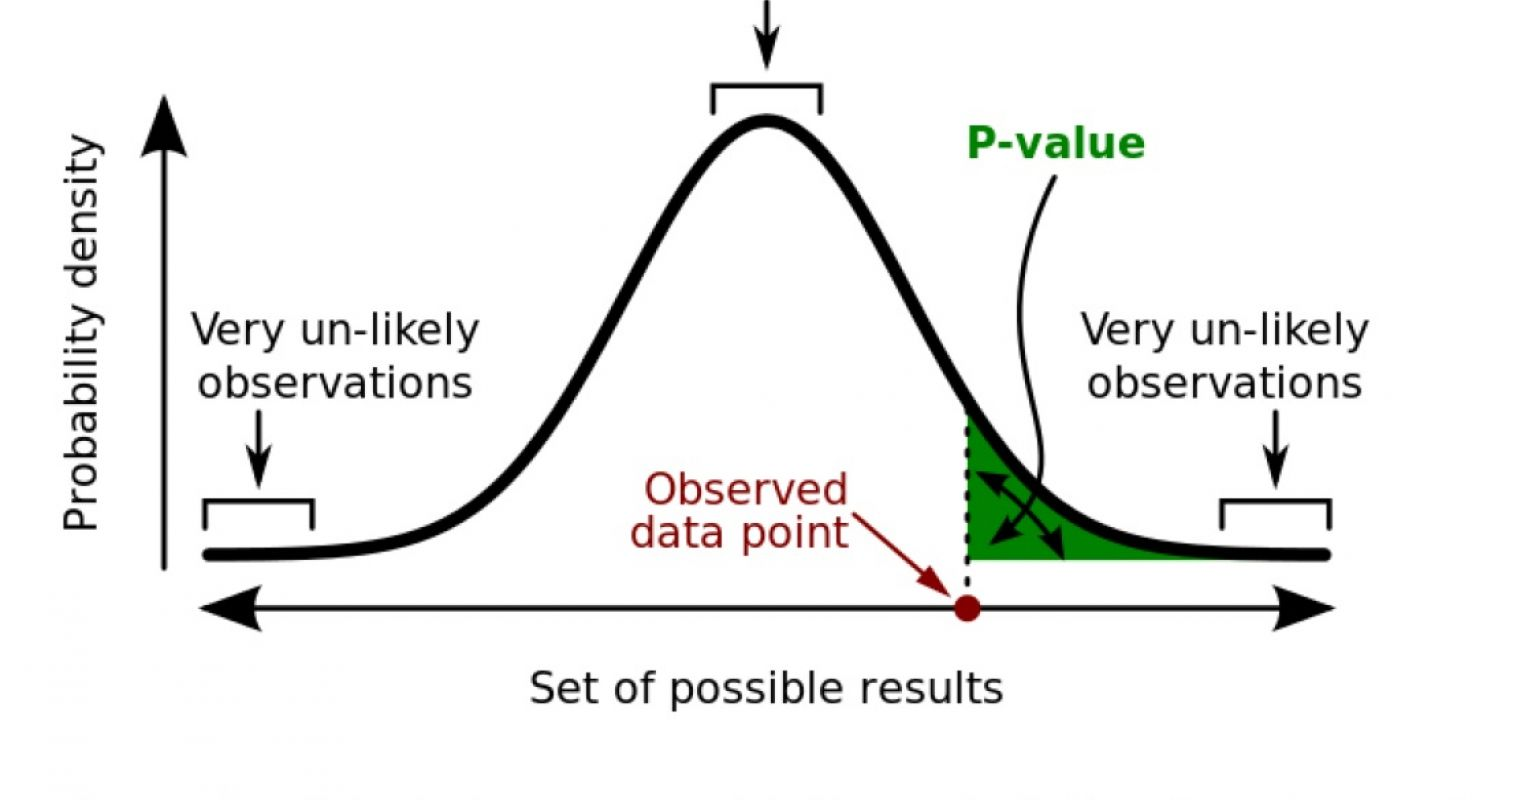
\includegraphics[width=0.8\textwidth]{
        images/06_Evaluation_pValue.jpg
    }
	\caption{p-value}
	\label{fig:p_value}
\end{figure}

\subsection{A useful digression to better understand hypothesis testing}
Suppose that $X_{1}, X_{2}, \hdots, X_{n}$ is a random sample sampled from a normal
distribution with parameters $\mu$ and $\sigma^{2}$. The variance of the normal
distribution is known, while the mean value is unknown. Given a plausible mean
value $\mu_{0}$, we want to test the null hypothesis:
\[
	H_{0}: \mu = \mu_{0}
\]

For example, if we are testing the performance differences between two machine
learning algorithms and the null hypothesis states that there is no difference
between the performance of the two algorithms, then the mean value of their difference
in performance would be 0.
\newline

In this case, $\Bar{X}:= \frac{1}{n}\sum_{i=1}^{n}X_{i}$ is the natural punctual
estimator for $\mu$. We accept $H_{0}$ when $\Bar{X}$ is not too far from
$\mu_{0}$. As a consequence, for a proper choice of the constant $c$, the critical
region is:
\begin{equation}
	\label{example_criticalRegion}C = \{(X_{1},X_{2},\hdots,X_{n}) : |\Bar{X}|-\mu_{0}
	|>c\}
\end{equation}
If our intention is to build a test with significance level $\alpha$, we need to
find the value of $c$ in Equation \ref{example_criticalRegion} such that the probability
of commit a first type error is $\alpha$. This means that $c$ has to verify the
following relation:
\begin{equation}
	\label{prob_1TypeErrorExample}\alpha = P(\mathit{I \; type \; error}) = P_{\mu_0}
	(|\Bar{X}-\mu_{0}|>c)
\end{equation}
We write $P_{\mu_0}$ to indicate the value of probability computed under the assumption
that $\mu = \mu_{0}$. Indeed, by definition, first type error occurs when the
sampled data lead us to reject $H_{0}$ (i.e. ($X_{1}, X_{2}, \hdots, X_{n}\in C$))
when indeed the null hypothesis is correct (i.e. $\mu=\mu_{0}$).\\ When
$\mu =\mu_{0}$, we know that $\Bar{X}$ is characterized by a normal distribution
with mean value $\mu_{0}$ and variance $\frac{\sigma^{2}}{n}$. Considering a
$\mathcal{N}(0,1)$ random variable $\mathcal{Z}$, we obtain:
\begin{equation}
	\frac{\Bar{X}-\mu_{0}}{\frac{\sigma}{\sqrt{n}}}\sim_{\mu_0}\mathcal{Z}
\end{equation}
Where the relation $\sim$ is conditioned to the hypothesis that: $H_{0}: \mu = \mu
_{0}$. The Equation \ref{prob_1TypeErrorExample} can now be written as:
\[
	\alpha = P_{\mu_0}(|\frac{\Bar{X}-\mu_{0}}{\frac{\sigma}{\sqrt{n}}}| > \frac{c
	\sqrt{n}}{\sigma}) = P(|Z| > \frac{c \sqrt{n}}{\sigma}) = 2P(Z > \frac{c
	\sqrt{n}}{\sigma})
\]
From this formula, we can immediately conclude that:
\[
	P(Z > \frac{c \sqrt{n}}{\sigma}) = \frac{\alpha}{2}
\]
By definition of $z_{\frac{\alpha}{2}}$ we write:
\[
	P(Z > z_{\frac{\alpha}{2}}) = \frac{\alpha}{2}
\]
From this we get:
\[
	\frac{c \sqrt{n}}{\sigma}= z_{\frac{\alpha}{2}}
\]
\[
	c = z_{\frac{\alpha}{2}}\frac{\sigma}{\sqrt{n}}
\]
We can conclude that:
\begin{itemize}
	\item if $|\frac{\Bar{X}-\mu_{0}}{\frac{\sigma}{\sqrt{n}}}|>z_{\frac{\alpha}{2}}$
		we reject $H_{0}$

	\item if $|\frac{\Bar{X}-\mu_{0}}{\frac{\sigma}{\sqrt{n}}}| \leq z_{\frac{\alpha}{2}}$
		we accept $H_{0}$
\end{itemize}
\begin{figure}[H]
	\centering
	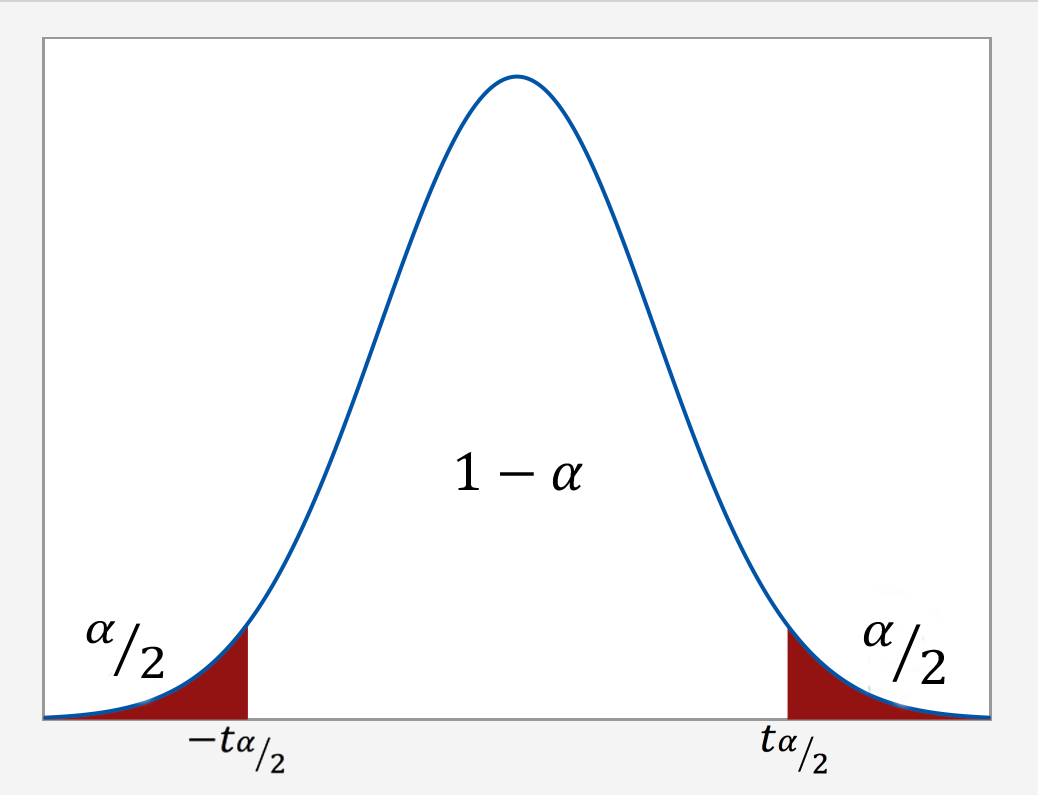
\includegraphics[width=0.5\textwidth]{
		images/06_Evaluation_normalDistributionTest.png
	}
	\caption{Confidence intervals}
	\label{fig:confidence_intervals}
\end{figure}

The acceptance region corresponds to the interval symmetric with respect to 0 labeled
with $1-\alpha$ in Figure \ref{fig:confidence_intervals}.

\subsection{Hypothesis testing when the variance is unknown}
Up to this point we have assumed that the only unknown parameter of the distribution
is the mean value. However, really often both the mean $\mu$ and the variance $\sigma
^{2}$ are unknown. Under these new assumptions, we study how to test the null hypothesis
about the mean value.
\[
	H_{0}: \mu = \mu_{0}
\]
Analogously to what we have done before, it is reasonable to reject the null hypothesis
when the sample mean $\Bar{X}$ is far from $\mu_{0}$. However, in this case the problem
is more difficult since the distance between $\Bar{X}$ and $\mu_{0}$ which determines
a rejection of the null hypothesis, depends on the standard deviation $\sigma$, which
in this new setting is unknown. In particular, in the previous case, the null
hypothesis is rejected when $|\Bar{X}-\mu_{0}|$ is larger then
$z_{\frac{\alpha}{2}}\cdot \frac{\sigma}{\sqrt{n}}$:
\[
	|\frac{\Bar{X}-\mu_{0}}{\frac{\sigma}{\sqrt{n}}}|>z_{\frac{\alpha}{2}}
\]
Since $\sigma$ is unknown, we replace it with the sample standard deviation $S$.
\begin{equation}
	S = \sqrt{\frac{1}{n-1}\sum_{i=1}^{n}(X_{i}-\Bar{X})^{2}}
\end{equation}
Given that, we reject the null hypothesis when
$|\frac{\Bar{X}-\mu_{0}}{\frac{S}{\sqrt{n}}}|$ is "too large". In order to understand
when this quantity is "too large" we need to know the distribution of the statistic
test when $H_{0}$ is verified.

\theo{\textbf{Probability distribution of a sample sampled from a Gaussian distribution with unknown variance}\label{theo:no_variance_gaussian}\\

$X_{1}, X_{2}, \hdots, X_{n}$ is a sample sampled from a Gaussian distribution with mean value $\mu$. If $\Bar{X}$ and $S^{2}$ denotes the sample average and the sample variance respectively, then: \begin{equation}\frac{\Bar{X}-\mu}{\frac{S}{\sqrt{n}}}\sim t_{n-1}\end{equation}

\begin{itemize}\item When we normalize $\Bar{X}$ by subtracting the mean value $\mu$ and dividing by the standard deviation $\frac{\sigma}{\sqrt{n}}$, we obtain a \textbf{standard normal distribution}.

\item When we normalize $\Bar{X}$ by subtracting the mean value $\mu$ and dividing by the sample standard deviation $\frac{S}{\sqrt{n}}$, we obtain a \textbf{Student's t-distribution} with $n-1$ degrees of freedom.\end{itemize} }

We denote the statistic of the test with $T$ such that:
\[
	T = \frac{\Bar{X}-\mu}{\frac{S}{\sqrt{n}}}
\]
Under the assumption that $H_{0}$ is true ($\mu = \mu_{0}$), $T$ is a $t$-distribution
with $n-1$ degrees of freedom. We impose that the probability of a type one
error is $\alpha$:
\[
	P_{\mu_0}(-c \leq \frac{\Bar{X}-\mu_{0}}{\frac{S}{\sqrt{n}}}\leq c) = 1 - \alpha
\]
\[
	\alpha = 1 - P(-c < T < c) = P(T \leq -c) + P(T \geq c) = 2P(T \geq c)
\]
\[
	P(T>c) = \frac{\alpha}{2}
\]
\[
	c = t_{\frac{\alpha}{2},n-1}
\]
In conclusion:
\begin{itemize}
	\item $H_{0}$ is rejected at a significance level $\alpha$ if:
		\[
			|\frac{\Bar{X}-\mu_{0}}{\frac{S}{\sqrt{n}}}|>t_{\frac{\alpha}{2},n-1}
		\]

	\item $H_{0}$ is accepted if:
		\[
			|\frac{\Bar{X}-\mu_{0}}{\frac{S}{\sqrt{n}}}|\leq t_{\frac{\alpha}{2},n-1}
		\]
\end{itemize}

In this case, the p-value is the probability that a Student's t-distribution
with $n-1$ degrees of freedom has a value larger then $|t|$ under the assumption
that $H_{0}$ is verified, where $t$ is the test statistic calculated from the sample
data.

\subsection{Some properties of the t distribution}
In the following we report some important properties of the $t_{k-1}$ distribution.
\begin{itemize}
	\item The Student's t-distribution is a bell-shaped distribution similar to the
		Normal one

	\item The shape is wider and shorter (fatter tails): reflects greater variance
		due to using its approximation $\tilde{Var}[\Bar{X}]$ instead of the true
		unknown variance of the distribution

	\item $k-1$ is the number of degrees of freedom of the distribution (related
		to the number of independent events observed)

	\item $t_{k-1}$ tends to the standardized normal $Z$ for $k \rightarrow \infty$
\end{itemize}

\section{Comparing learning algorithms}
The purpose of this section is to understand how to compare two learning algorithms
using hypothesis testing.\\ First of all we run k-fold cross validation procedure
for algorithms A and B. Then we compute the mean performance difference for the
two algoritms:
\begin{equation}
	\hat{\delta}= \frac{1}{k}\sum_{i=1}^{k}\delta_{i}= \frac{1}{k}\sum_{i=1}^{k}S_{\mathcal{D}_i}
	[L_{A}(\mathcal{T}_{i})] - S_{\mathcal{D}_i}[L_{B}(\mathcal{T}_{i})]
\end{equation}

Where $S_{\mathcal{D}_i}[L_{A}(\mathcal{T}_{i})]$ is the performance of
algorithm A on fold $i$. In particular the learning algorithm $L_{A}$ is executed
on a subset of the dataset ($\mathcal{T}_{i}$) while the performance ($S$) of the
algorithm is measured considering the rest of the dataset ($\mathcal{D}_{i}$).
\newline

The null hypothesis is that the mean difference is zero (i.e. there is no difference
between the two algorithms).
\[
	H_{0}: \mu = 0
\]

Clearly, the variance of the distribution is unknown. As a consequence we
implement a t-test which rejects the null hypothesis at significance level
$\alpha$ when:
\[
	\frac{\Bar{\delta}}{\sqrt{\tilde{Var}[\Bar{\delta}]}}\leq - t_{k-1, \frac{\alpha}{2}}
\]
or
\[
	\frac{\Bar{\delta}}{\sqrt{\tilde{Var}[\Bar{\delta}]}}\geq t_{k-1, \frac{\alpha}{2}}
\]
where $\Bar{\delta}$ is the sample mean of the difference and:
\[
	\sqrt{\tilde{Var}[\Bar{\delta}]}= \sqrt{\frac{1}{k(k-1)}\sum_{i=1}^{k}(\delta_{i}-
	\Bar{\delta})^{2}}
\]
Notice the the null hypothesis assumes zero means, that is why $\Bar{\delta}$ is
alone in the numerator.
\newline
We perform a two-tailed test if no prior knowledge can tell the direction of the
difference. Otherwise it is reasonable to use one-tailed test.
\subsection{t-test example: 10-fold cross validation}
In Figure \ref{fig:tTestExample} there are reported the test performances
computed on ten folds. The first column is the number of the fold ($\mathcal{D}_{1}
, \mathcal{D}_{2}, \hdots, \mathcal{D}_{10}$) of the 10-fold cross validation.
The second and the third columns reports the performances (e.g. accuracy) achieved
by algorithm A and B respectively. Finally, the fourth columns indicates the difference
between the two scores.\\ Firstly, we can easily compute the mean value of the
difference:
\[
	\Bar{\delta}= \frac{1}{10}\sum_{i=1}^{10}\delta_{i}= 0.046
\]

\begin{figure}[H]
	\centering
	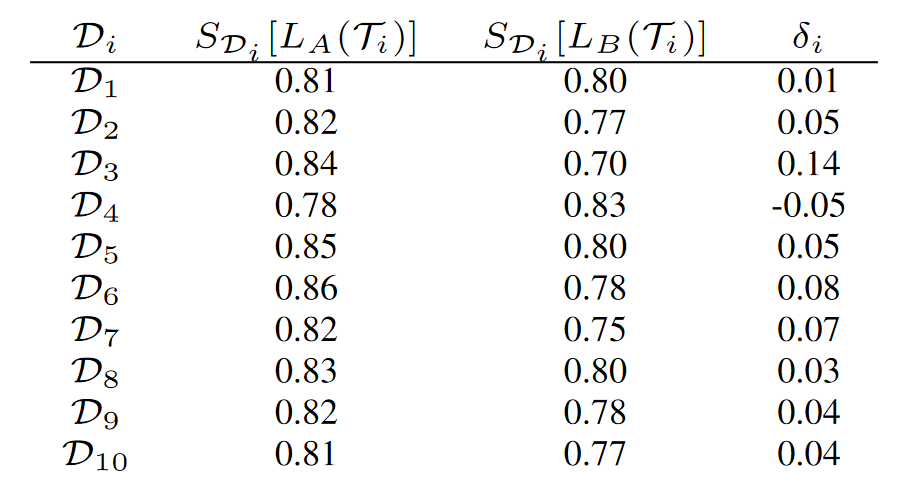
\includegraphics[width=0.8\textwidth]{
        images/06_Evaluation_tTest.png
    }
	\caption{10-fold cross validation used to implement a t-test example on the
	performance difference between two algorithms A and B.}
	\label{fig:tTestExample}
\end{figure}

At this point we compute the unbiased estimate of the standard deviation:
\[
	\sqrt{\tilde{Var}[\Bar{\delta}]}= \sqrt{\frac{1}{10 \cdot 9}\sum_{i=1}^{10}(\delta_{i}-
	\Bar{\delta})^{2}}= 0.0154344
\]
With this value we can calculate the standardized mean error difference:
\[
	\frac{\Bar{\delta}}{\sqrt{\tilde{Var}[\Bar{\delta}]}}= \frac{0.046}{0.0154344}=
	2.98
\]
We compute the $t$ distribution for $\alpha=0.05$ (i.e. we are happy to have a type
one error probability of $5\%$) (it is a two-tailed test so we consider $\frac{\alpha}{2}$
in the following formula) and $k=10$:
\[
	t_{k-1, \frac{\alpha}{2}}= t_{9,0.025}= 2.262
\]
Finally, since $2.262 < 2.98$, the null hypothesis is rejected. We can conclude
that the two classifiers are different. Indeed, my observation (i.e. my test
statistic) is further to the right with respect to $t_{k-1, \frac{\alpha}{2}}$.
In order to calculate the value of $t_{9,0.025}$ we have looked at the entry
$[d f = 9, t_{.}025]$ of the table in Figure \ref{fig:tDistributionTable}.
\newline

\begin{figure}[H]
	\centering
	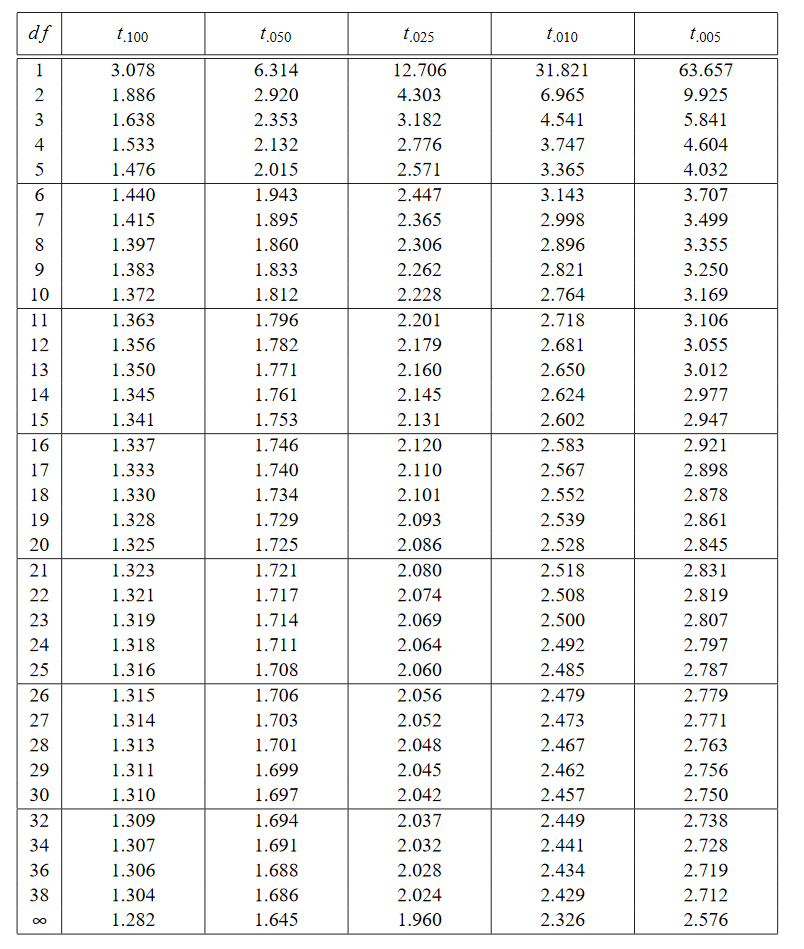
\includegraphics[width=0.6\textwidth]{
        images/06_Evaluation_tDistribution.png
    }
	\caption{Computing Student's t distribution.}
	\label{fig:tDistributionTable}
\end{figure}

\textbf{Remarks:}
\begin{itemize}
	\item The test we have described in this section is a \textit{paired test}
		since both the algorithms are evaluated over identical samples.

	\item The test we have described is a \textit{two-tailed test}. Indeed we can not
		tell a priory if algorithm A is better then B or vice versa. Otherwise, if we
		had prior knowledge about the direction of the difference, we would use a
		one-tailed test (dividing $\alpha$ by two wouldn't be required).
\end{itemize}
    \chapter{Parameter estimation}

\label{cha:param_estimation}

The settings of the environment we are now working in rely on:
\begin{itemize}
    \item a collection of data sampled from a probability distribution $p(\pmb{x}, y)$
    \item the probability distribution $p(\pmb{x}, y)$ from which data are driven is known, but the parameters that describe this distribution are unknown (e.g. we know that $p$ is a Gaussian distribution but we do not know the actual mean $\mu$ and variance $\sigma$ (or mean vector and covariance matrix in the multivariate case)
    \item the data coming from the training set $\mathcal{D} = \{(\pmb{x}_1, y_1), \dots, (\pmb{x}_m, y_m)\}$ are independent and identically distributed samples (i.i.d.) according to $p(\pmb{x}, y)$
    \item the training set $\mathcal{D}$ can be divided into $\mathcal{D}_1, \dots, \mathcal{D}_c$ subsets, with $c$ equal to the number of classes. For each subset we have $n$ examples i.i.d. $\mathcal{D}_i = \{\pmb{x}_1, \dots, \pmb{x}_n\}$
    \item for any \textit{new} example $x$ not in the training set, we compute the posterior probability of the class given the example and the full training set
    $\mathcal{D}$:
    \begin{equation}
    P(y_i|\pmb{x}, \mathcal{D}) = \frac{p(\pmb{x}|y_i, \mathcal{D})p(y_i|\mathcal{D})}{p(\pmb{x}|\mathcal{D})}
    \label{eq:main_eq}
    \end{equation}
    
    Computing this process for every class, we can take as predicted label the maximum probability among the classes.
\end{itemize}

\sumup{We are trying to find the parameters that describe the actual distribution $p$ from the training data $\mathcal{D}$, therefore $p(\pmb{X} | \mathcal{D}_i, y_i)$.}

From now on, whenever we are referring to a vector of features, we will use the bold notation $\pmb{x}$.

\defi{By \textit{independent} we mean that each example is sampled independently from the others.}
\defi{By \textit{identically distributed} we mean that all examples are sampled from the same distribution $p(\pmb{x}, y)$.}

From these settings we can further assume some simplifications: 
\begin{itemize}
    \item $\pmb{x}$ is independent of $\mathcal{D}_j (j \neq i)$ given $y_i$ and $\mathcal{D}_i$
    $$P(y_i|\pmb{x}, \mathcal{D}) = \frac{p(\pmb{x}|y_i, \mathcal{D}_i)p(y_i|\mathcal{D})}{p(\pmb{x}|\mathcal{D})}$$
    \item without further knowledge
    $$p(y_i | \mathcal{D}) = \frac{\#y_i}{\#total} = \frac{|\mathcal{D}_i|}{|\mathcal{D}|}$$
    \item the normalizing factor $$p(\pmb{x}, \mathcal{D}) = \sum_{i=1}^c p(\pmb{x}|y_i, \mathcal{D}_i)p(y_i|\mathcal{D})$$
\end{itemize}

At this point, the factor of the Equation \ref{eq:main_eq} we are missing is $p(\pmb{x}|y_i, \mathcal{D}_i)$. In order to do this, we need to estimate the parameters $\theta_i$ of the given distribution.\\
There are two main option in order to get an estimation of the parameters $\theta_i$:
\begin{enumerate}
    \item \textbf{Maximum likelihood}: we assume that $\Theta_i$ have fixed but unknown values, then we assume that the parameters $\Theta_i$ are the ones that maximize the probability of the observed examples $\mathcal{D}_i$ (coming from the training set) of being part of $\mathcal{D}_i$.\\
    The values $\Theta_i$ are used to compute probability for new unseen examples:
    $$P(\pmb{x}|y_i, \mathcal{D}_i) \approx p(\pmb{x}|\Theta_i)$$
    \item \textbf{Bayesian estimation}: we assume that $\Theta_i$ are \textbf{not} fixed, but random variables with some known \textit{prior distribution}, as we observe examples, the prior distribution become a \textit{posterior} distribution. The prediction for the new examples are obtaining by an integral over the possible values of $\Theta_i$
    $$p(\pmb{x}|y_i, \mathcal{D}_i) = \int_{\Theta_i} p(\pmb{x}, \Theta_i|y_i, \mathcal{D}_i) d\Theta_i$$
\end{enumerate}

\section{Maximum-likelihood estimation}
    \label{par:maximum_likelihood_estim}
    This method of parameter estimation is based on an analysis \textit{a posteriori}, aka the data have already been seen.\\
    The estimation of the parameters $\Theta^*$ if the distribution $p(\pmb{x}, y)$ is based on finding the combination that fits at best the distribution of the data in each true class.
    $$\Theta_i^* = argmax_{\Theta_i} p(\Theta_i|\mathcal{D}_i, y_i) = argmax_{\Theta_i} \frac{p(\mathcal{D}_i, y_i|\Theta_i)p(\Theta_i)}{p(\mathcal{D}_i, y_i)}$$
    but $p(\mathcal{D}_i, y_i)$ does not depend on $\Theta$, so:
    $$\Theta_i^* = argmax_{\Theta_i} p(\Theta_i|\mathcal{D}_i, y_i) = argmax_{\Theta_i} p(\mathcal{D}_i, y_i|\Theta_i)p(\Theta_i)$$
    $p(\mathcal{D}_i, y_i|\Theta_i)$ is called the likelihood. $p(\Theta_i)$ is called the prior.\\
    This estimation assumes that a prior distribution for the parameters $p(\Theta_i)$ is available.\\
    The most common formulation for the maximum likelihood estimation is:
    \begin{equation}
        \Theta_i^* = argmax_{\Theta_i} p(\mathcal{D}_i, y_i| \Theta_i)
        \label{eq:max_likelihood_common}
    \end{equation}
    which maximizes the likelihood of the parameters with respect to the training samples\textbf{ without } prior knowledge distribution of the parameters.\\
    
    Since every class is treated independently, we will drop the redundant notation $\mathcal{D}_i, y_i$ with $\mathcal{D}$ since it is not ambiguous.\\
    
    With these assumption, we are trying to find $\theta^*$ as the combination of parameters for the distribution $p(x, y)$ that maximize the probability of a data coming for that same distribution:
    \begin{align*}
		\Theta^* &= argmax_{\Theta} p(\mathcal{D} | \Theta)\\
		&= argmax_\Theta \prod_{j=1}^n p(\pmb{x}_j|\Theta)
	\end{align*}
	
	\textbf{Remark:}
	$p(\mathcal{D}| \Theta) = \prod_{j=1}^n p(\pmb{x}_j|\Theta)$ since the elements $\pmb{x}_1, \hdots, \pmb{x}_n$ in the training data are i.i.d..
    
    \subsection{Maximizing the log-likelihood}
        In order to maximize the probability previously described, is it clever to consider to maximize the logarithm of the probability.
        This is considered useful because the log function is monotonic and has several properties that simplify the procedure. For instance, computing the derivatives of a product is a pain, while it is easier to derive a summation.
        
        \begin{align*}
    		\Theta^* &= argmax_{\Theta} \log p(\mathcal{D} | \Theta)\\
    		&= argmax_\Theta \sum_{j=1}^n \log p(\pmb{x}_j|\Theta)
    	\end{align*}    
        
        In order to get the maximum, we can apply the derivative operation and look for the null point of this function. Since there are several parameters we are looking for, we will apply a gradient to the equation:
        
        \begin{equation}
            \nabla _\Theta \sum_{j=1} ^n \log p(\pmb{x}_j|\Theta) = 0
        \end{equation}
        
        These point will be local or global maxima depending on the distribution.\\
        
        The distribution we take into account is a Gaussian \ref{def:gaussian_normal} distribution of the parameters $\mu$ and $\sigma$ (\textit{univariate} case).
        $$p(\pmb{x}_j|\Theta) = \frac{1}{\sqrt{2\pi}\sigma} \exp{(-\frac{(\pmb{x}-\mu)^2}{2\sigma ^2})} $$
        
        Considering the logarithm:
        $$\sum_{i=1}^n \log p(\pmb{x}_j|\Theta) = \sum_{i=1}^n \log{ \left[ \frac{1}{\sqrt{2\pi}\sigma} \exp{(-\frac{(\pmb{x}-\mu)^2}{2\sigma ^2})} \right] } = \sum_{i=1}^n \log{ \frac{1}{\sqrt{2\pi}\sigma}}-\frac{(\pmb{x}-\mu)^2}{2\sigma ^2}$$
        
        Let's begin with the derivative of the log of the probability with respect to $\mu$.
        
        \begin{align*}
        \pdv {p(\pmb{x}_j|\Theta)}{\mu} &= \pdv{}{\mu} \sum_{i=1}^n \log \frac{1}{\sqrt{2\pi}\sigma} - \frac{(\pmb{x}-\mu)^2}{2\sigma^2}\\
    	&= \sum_{i=1} ^n \frac{(\pmb{x}_i - \mu)}{\sigma^2}
    	\end{align*}
    	
    	If we set this quantity to be equal to zero we get
    	
    	\begin{align*}
        	\sum_{i=1}^n \frac{(\pmb{x}_i - \mu)}{\sigma^2} &= 0\\
        	\sum_{i=1}^n (\pmb{x}_i - \mu) &= 0\\
        	\sum_{i=1}^n \pmb{x}_i &= \sum_{i=1}^n \mu\\
        	\sum_{i=1}^n \pmb{x}_i &= n \mu\\
        	\mu &= \frac{1}{n}\sum_{i=1}^n \pmb{x}_i
    	\end{align*}
    	
    	\textbf{Remark:} this is the sample mean. \newline
    	
    	Repeating these operation with respect to $\sigma$ we get	
    	
    	\begin{align*}
    	\pdv {p(\pmb{x}_j|\Theta)}{\sigma} &= \pdv{}{\sigma} \sum_{i=1}^n \log \frac{1}{\sqrt{2\pi}\sigma} - \frac{(\pmb{x}_i-\mu)^2}{2\sigma^2}\\
    	&= \sum_{i=1} ^n \sqrt{2 \pi} \sigma \frac{1}{\sqrt{2 \pi}}(- \sigma^{-2})-\frac{(\pmb{x}_i - \mu)^2}{2} (-2 \sigma^{-3}) \\
    	&= \sum_{i=1} ^n -\frac{1}{\sigma} + \frac{(\pmb{x}_i - \mu)^2}{\sigma^3}
    	\end{align*}
    	
    	If we set this quantity to be equal to zero we get
    	
    	\begin{align*}
    	    \sum_{i=1} ^n -\frac{1}{\sigma} + \frac{(\pmb{x}_i - \mu)^2}{\sigma^3} &= 0\\
        	\sigma^3 \cdot \sum_{i=1} ^n -\frac{1}{\sigma} + \frac{(\pmb{x}_i - \mu)^2}{\sigma^3} &= 0 \cdot \sigma^3\\
        	\sum_{i=1}^n -\sigma^2 + \sum_{i=1}^n (\pmb{x}_i - \mu^2) &= 0\\
        	\sum_{i=1}^n (\pmb{x}_i - \mu^2) &= \sum_{i=1}^n \sigma^2\\
        	\sum_{i=1}^n (\pmb{x}_i - \mu^2) &= n \sigma^2\\
        	\sigma^2 &= \frac{\sum_{i=1}^n (\pmb{x}_i - \mu)^2}{n}
    	\end{align*}
    	
    	\textbf{Remark:} this is the sample variance. \newline
    	
    	By this we can get to the conclusion that if take into account Gaussian distribution, then the parameters that maximize the fitting of the training data into the dataset divided per class correspond to the sample mean and to the sample variance.
    	
    	\sumup{
    	If this example is valid for a univariate (single feature) Gaussian distribution, we can extend the concept to a multivariate Gaussian distribution \ref{def:multi_normal_dist} and get as a result that:
    	\begin{itemize}
    	    \item the log of the likelihood is
    	    $$\sum_{j=1}^n -\frac{1}{2} (x_j - \mu)^t \Sigma^{-1}(x_j - \mu) -\frac{1}{2}log(2\pi)^d|\Sigma|$$
    	    \item the maximum likelihood estimates are the vector of the sample means
    	    $$\mu = \frac{1}{n}\sum_{j=1}^n x_j$$
    	    and the covariances matrix
    	    $$\Sigma = \frac{1}{n} \sum_{j=1}^n (x_j - \mu)(x_j - \mu)^t$$
    	\end{itemize}
    	
    	In the general case of a Gaussian distribution the maximum likelihood parameters are simply their empirical estimates over the samples.\\
    	The Gaussian mean is the sample mean while the covariance matrix is the mean of the sample covariances.}
    	
\section{Bayesian estimation}
    \label{par:Bayesian_estimation}
    With this approach we focus on the estimation of the parameters of our distribution $p(x, y)$ a \textit{priori}, meaning that we update our values while getting new classified data.\\
    In this case, the parameters $\Theta_i$ are related to a random variables (with some known prior distribution) that also need to be modeled. The prediction of the new samples is obtained through the integral over every possible parameter.
    $$p(x|y_i, \mathcal{D}_i) = \int_{\Theta_i} p(x, \Theta_i|y_i, \mathcal{D}_i) d\Theta_i$$
    The probability of $\pmb{x}$ given each class $y_i$ is independent of the other classes $y_j$ with $i \neq j$. For simplicity we write:
    $$p(\pmb{x}|\mathcal{D}) = \int_{\Theta} p(\pmb{x}, \Theta|\mathcal{D}) d\Theta$$
    $$p(\pmb{x}|\mathcal{D}) = \int_{\Theta} p(\pmb{x} |\Theta,\mathcal{D}) p(\Theta | \mathcal{D}) d\Theta$$ 
    where $\mathcal{D}$ is the dataset for a certain class $y$ and $\Theta$ the parameters of its distribution.\\
    
    Let's proceed also in this case considering a Gaussian \ref{def:gaussian_normal} distribution with unknown parameters $\Theta$.\\
    In computing $p(\pmb{x} | \Theta, \mathcal{D})$, we do not need $\mathcal{D}$ since the probability of an example depends only on the parameters $\Theta$. As a result, hereafter we write $p(\pmb{x}|\Theta)$.
    Since the prediction is conditioned on the parameters $\Theta$
    $$p(\pmb{x}|\mathcal{D}) = \int p(\pmb{x}|\Theta)p(\Theta|\mathcal{D})d\Theta$$
    The member of the equation $p(\pmb{x}|\Theta)$ can be easily compute since we have the type of distribution and its parameters.
    Therefore we need to estimate the parameter posterior density given the training set:
    $$p(\Theta|\mathcal{D}) = \frac{p(\mathcal{D}|\Theta)p(\Theta)}{p(\mathcal{D})}$$
    In this formula $p(\mathcal{D})$ is a constant independent on $\Theta$ (therefore will not influence the Bayesian decision).
    If the final probability is needed we can compute it through
    $$p(\mathcal{D}) = \int_{\Theta} p(\mathcal{D}|\Theta)p(\Theta)d\Theta$$
    
    \textbf{Remark:} Calculating $p(\mathcal{D})$ is useful only if we want the final probability. Otherwise, if we only need to compute the most probable class then $p(\mathcal{D})$ can be treated as a constant and it is not necessary to compute it.
    
    \subsection{Univariate normal case: unknown \texorpdfstring{$\mu$}{u} and known \texorpdfstring{$\sigma$}{s}}
    In the following we consider a univariate normal case such that the mean $\mu$ is unknown and the standard deviation is known. In other words $\Theta = \{ \mu \}$.
    Let's say that we are trying to define $\mu$ from a given Gaussian distribution $p(x|\Theta) = p(x|\mu) \sim \mathcal{N}(\mu, \sigma^2)$.
    For the Bayesian settings in which we are working, also the mean $\mu$ belongs to a Gaussian distribution $p(\mu) \sim \mathcal{N}(\mu_0, \sigma_{0}^2)$: this distribution derives from \textbf{prior} knowledge, $\mu$ is at this time a random variable. For example, $\mu$ could be a random variable representing the mean height of the German student at the University of Trento while the prior $\mu_0, \sigma^2_0$ could be the mean and the variance of the world German population.\\
    The Gaussian mean posterior given the dataset is computed as
    \begin{align*}
    p(\mu|\mathcal{D}) &= \frac{p(\mathcal{D}|\mu)p(\mu)}{p(\mathcal{D})}\\
    &= \alpha \prod_{j=1}^n p(x_j|\mu)p(\mu)
    \end{align*}
    where $\alpha = \frac{1}{p(\mathcal{D})}$ is independent of $\mu$.\\
    
    $p(\mathcal{D}|\mu)=\prod_{j=1}^n p(\pmb{x}_j|\mu)$ since the examples are i.i.d..\\
    
    From here we compute $p(\mu|\mathcal{D})$ taking into account two Gaussian distributions: the Gaussian distribution (of the data) $p(\pmb{x}_j | \mu) \sim \mathcal{N}(\pmb{x}_j ; \mu, \sigma^2)$ and the one for of the mean, $p(\mu) \sim \mathcal{N}(\mu ; \mu_0, \sigma_{0}^2)$.\\
    After some mathematical computation (substituting the definition of normal distribution we get), we get that $p(\mu;\mathcal{D})$ is equal to
    $$p(\mu | D) = \alpha \prod_{i=1}^n \frac{1}{\sqrt{2 \pi} \sigma} \mathit{exp} - \frac{(\pmb{x}_i-\mu)^2}{2 \sigma^2} \frac{1}{\sqrt{2 \pi} \sigma_0} \mathit{exp} - \frac{(\mu - \mu_0)^2}{2 \sigma_0^2}$$
    Which, after some manipulations, becomes:
    \begin{figure}[H]
        \centering
        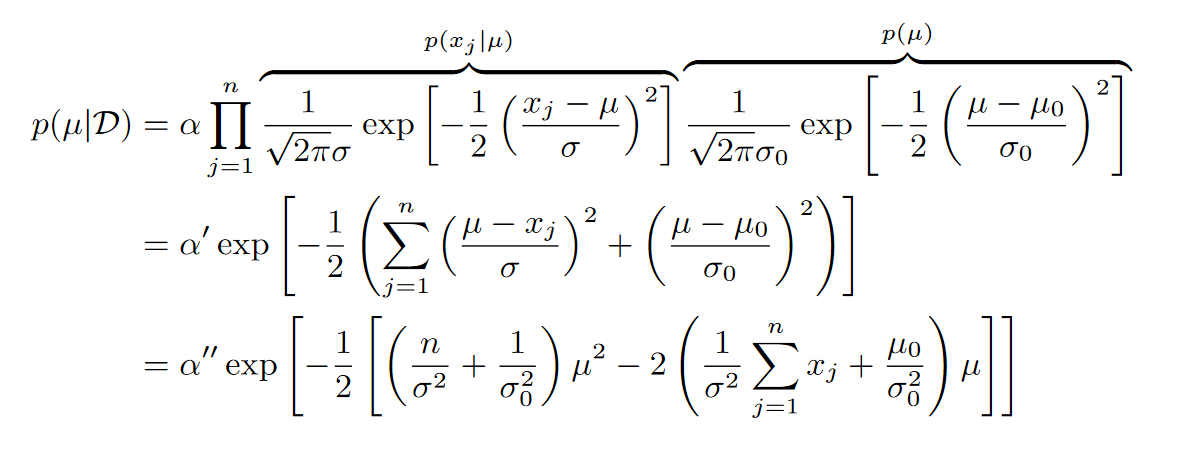
\includegraphics[scale=0.4]{images/bayesian_univariate_gaussian_inter_calculus.png}
    \end{figure}
    From the last step, we can see that this composition behaves like a normal distribution itself
    $$p(\mu|\mathcal{D}) = \frac{1}{\sqrt{2\pi}\sigma_n} e^{\frac{1}{2} (\frac{(\mu - \mu_n)}{\sigma^n})^2}$$
    then we can put the last two equation as equal (the step by step explanation is omitted). 
    
    Solving for $\mu_n$ and $\sigma_n^2$ we get
    $$\mu_n = \left( \frac{n\sigma_0^2}{n\sigma_0^2 + \sigma^2} \right)  \hat{\mu_n} + \frac{\sigma^2}{n\sigma_0^2 + \sigma^2} \mu_0$$
    and
    $$\sigma_n^2 = \frac{\sigma_0^2\sigma^2}{n\sigma_0^2 + \sigma^2}$$
    where $\hat{\mu_n}$ is the sample mean
    $$\hat{\mu_n} = \frac{1}{n} \sum_{j=1}^n x_i$$
    
    The interpretation of these results are the following:
    \begin{itemize}
        \item the mean is a \textbf{linear combination} of the \textit{prior} $\mu_0$ and the sample mean $\hat{\mu}_n$
        \item the higher the number of the training sample $n$, the more importance gets the sample mean $\hat{\mu}_n$, while $\mu_0$ loses importance
        \item the more training samples $n$ the more the variance decreases making the distribution less uncertain and more sharp.
    \end{itemize}
    
    \begin{figure}[H]
        \centering
        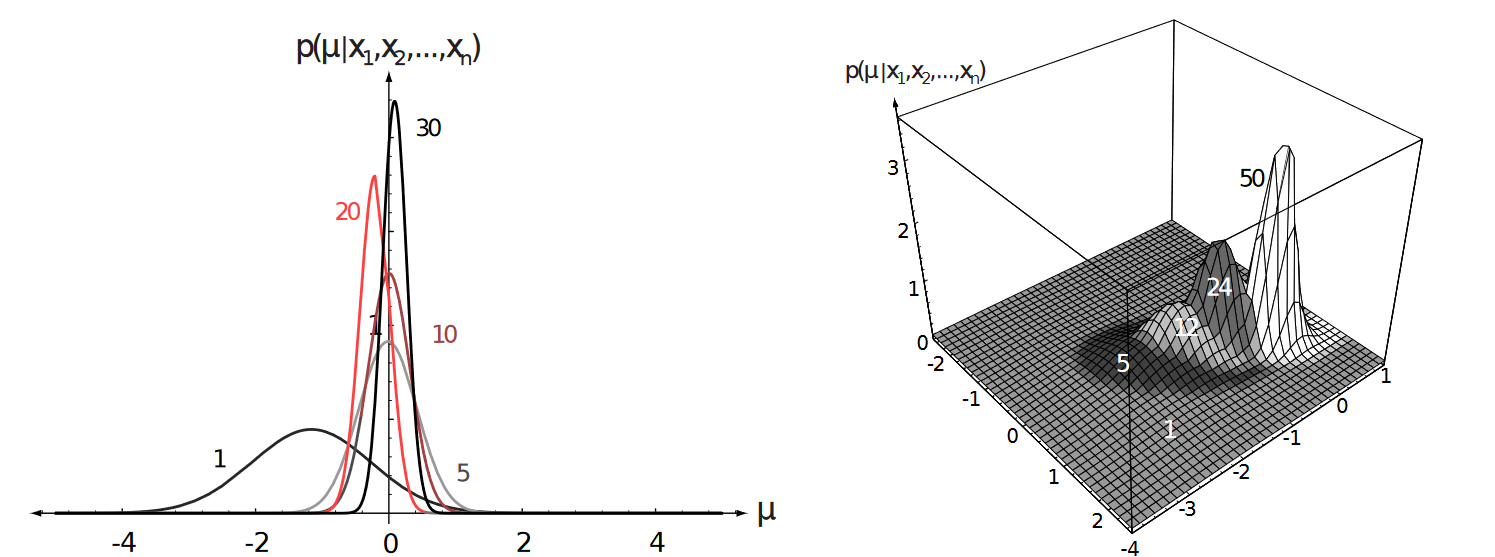
\includegraphics[scale=0.3]{images/bayesian_estimation.png}
        \caption{2D and 3D graphics of increasing number of $n$ samples seen for a Bayesian estimation of the mean $\mu$}
        \label{fig:bayesian_mean_estimate}
    \end{figure}
    
    \sumup{
    By this, we get that 
    $$p(x|\mathcal{D}) \sim \mathcal{N}(\mu_n, \sigma^2 + \sigma_n^2)$$
    therefore the Gaussian distribution of the probability for the new samples in the model is built with parameters $\Theta$ that are the mean (as the posterior mean) and the sum of the known variance and the variance of the mean as a random variable (aka the uncertainty over the mean.
    }
    
    \subsection{Generalization of univariate case}
    Since we know that
    $p(x|\mu) \sim \mathcal{N}(\mu, \Sigma)$\\
    $p(\mu) \sim \mathcal{N}(\mu_n, \Sigma_n)$\\
    therefore
    $p(\mu|\mathcal{D}) \sim \mathcal{N}(\mu_n, \Sigma_n)$\\
    and
    $p(x|\mathcal{D}) \sim \mathcal{N}(\mu_n, \Sigma + \Sigma_n)$
    
\section{Sufficient statistics}
    \defi{\textbf{Statistic}\label{def:statistic}\\
    Any function on a set of samples $\mathcal{D}$ is a statistic, a sufficient statistic
    $$\textbf{s} = \Phi(\mathcal{D})$$
    respects the following statement:
    $$P(\mathcal{D}|\textbf{s}, \Theta) = P(\mathcal{D}|\textbf{s})$$
    If $\Theta$ is a random variable, a sufficient statistic \textbf{s} contains all the relevant information about $\mathcal{D}$ in order to get the same and correct probability:
    $$p(\Theta|\mathcal{D}, \textbf{s}) = \frac{p(\mathcal{D}| \Theta, \textbf{s})p(\Theta|\textbf{s})}{p(\Theta|\textbf{s})} = p(\Theta|\textbf{s})$$
    }
    A sufficient statistic for a Gaussian distribution are sample mean and covariance. 
    
\section{Conjugate priors}
    \defi{\textbf{Conjugate prior}\label{def:conj_prior}\\
    Given the likelihood function $p(x|\Theta)$ and the prior distribution $p(\Theta)$, then
    $$p(\Theta)$$
    is a conjugate prior for $p(x|\Theta)$ if the posterior distribution $p(\Theta|x)$ is in the same family as the prior $p(\Theta)$
    }
    
    \begin{table}
        \centering
        \begin{tabular}{|c|c|c|}
            \hline
            \textbf{likelihood} & \textbf{Parameters} & \textbf{Conjugate prior}  \\
            \hline
            Binomial & p (\textit{probability}) & Beta  \\
            \hline
            Multinomial & p (\textit{probability vector}) & Dirichlet \\
            \hline
            Normal & $\mu$ (\textit{mean}) & Normal \\
            \hline
            Multivariate Normal & $\mu_i$ (\textit{mean vector}) & Normal \\
            \hline
        \end{tabular}
        \caption{examples of distributions and their conjugate priors}
        \label{table:conj_priors}
    \end{table}
    
    In Table \ref{table:conj_priors} we report some examples of distributions and their conjugate priors.\\

    \subsection{Example of a Bernoulli distribution}
        Given a Bernoulli distribution \ref{defi:bernoullo_dist} with events $x=1$ for \textit{success} and $x=0$ for \textit{failure}, parameters $\Theta$ for success and $1-\Theta$ for failure and probability mass distribution 
        $$P(x|\Theta) = \Theta^x(1-\Theta)^{1-x}$$
        then the conjugate prior is a Beta distribution \ref{def:beta_dist} that depends on $\alpha_h, \alpha_t$
        \begin{align*}
        P(\Theta|\psi)  &= P(\Theta|\alpha_h, \alpha_t)\\
                        &= \frac{\Gamma(\alpha)}{\Gamma(\alpha_h)\Gamma(\alpha_t)} \Theta^{\alpha_h -1} (1-\Theta)^{\alpha_t -1}
        \end{align*}
        
        \subsubsection{Maximum likelihood estimation}
        \label{par:maximum_likelyhood_estim}
            For example, we can prove that given a dataset $\mathcal{D} = \{H, H, T, T, T, H, H\}$ of $N$ iterations (like head/tail toss results), then the likelihood function becomes
            $$p(\mathcal{D}|\Theta) = \Theta^h(1-\Theta)^t$$
            The maximum likelihood parameter (maximizing the probability means compute the gradient and zeroing it), we are interested in the derivation with respect to $\Theta$, then the estimation becomes
            \begin{align*}
                \pdv{}{\Theta} \log p(\mathcal{D}| \Theta) \longrightarrow \pdv{}{\Theta}h\log \Theta + t \log(1-\Theta) &= 0\\
                h\frac{1}{\Theta} - t\frac{1}{1-\Theta} &= 0\\
                h(1-\Theta) &= t\Theta\\
                \Theta &= \frac{h}{h+t}
            \end{align*}
            By this we mean that $t, h$ are a sufficient statistic \ref{def:statistic}. The best maximum likelihood parameters is the number of successes in the data among the total.
        
        \subsubsection{Bayesian estimation}
            If we try to estimate the parameters through a Bayesian estimation \ref{par:Bayesian_estimation}, then the conjugate prior will still be a Beta distribution \ref{def:beta_dist}.\\
            The posterior is proportional to $P(\mathcal{D}|\Theta)P(\Theta|\psi)$ which comes from the Bayes' theorem \ref{theo:bayes} where $P(\mathcal{D})$ is omitted (therefore the $\propto$ property and not $=$), but it is also proportional to $P(\mathcal{D}|\Theta)P(\Theta,\psi)$ which is the prior Beta distribution
            \begin{align*}
                P(\Theta|\mathcal{D}, \psi) &\propto P(\mathcal{D}|\Theta)P(\Theta|\psi)\\
                &\propto \Theta^h (1-\Theta)^t \Theta^{\alpha_h -1} (1-\Theta)^{\alpha_t -1}
            \end{align*}
            This proportions gets together very easily collecting parameters until
            $$P(\Theta|\mathcal{D},\psi) \propto \Theta^{h+\alpha_h -1} (1 - \Theta)^{t + \alpha_t -1}$$
            that is a Beta distribution $\sim Beta(\alpha_h ',\alpha_t ')$ where parameters $\alpha_h '= h+\alpha_h$ and $\alpha_t ' = t + \alpha_t$. 
            The posterior of my parameters is again a Beta with a new pair of parameters $\alpha_h '$ and $\alpha_t '$ which are derived from the sum of the real counts ($h, t$) and the \textit{imaginary} counts ($\alpha_t, \alpha_h$).\\
            
            Then the prediction for a new event given the data is the expected value of the posterior Beta:
            \begin{align*}
                P(x|\mathcal{D})    &= \int_\Theta P(x,\Theta|\mathcal{D})d\Theta\\
                                    &= \int_\Theta P(\Theta|\mathcal{D}) P(\Theta|\mathcal{D})d\Theta
            \end{align*}
            Since we need to integrate on a binary output (success, fail), then let's focus of the success event ($P(x=1) =\Theta$) keeping in mind that $\Theta$ is a Beta distribution (therefore its expected value is $E[\Theta] = \frac{\alpha_h '}{\alpha_h ' + \alpha_t '}$):
            \begin{align*}
                P(x = 1 | \mathcal{D}) & = \int_\Theta \Theta P(\Theta|\mathcal{D}, \psi) d\Theta\\
                &= E[\Theta]\\
                &= \frac{h + \alpha_h}{h + t + \alpha_h + \alpha_t}
            \end{align*}
            by this we get that: 
            \begin{itemize}
                \item with high $t, h$ (seen results) then the parameters $\alpha_t, \alpha_h$ become irrelevant, so this estimation becomes closer to the maximum likelihood estimation,
                \item with small $t, h$ (seen results) that the prior estimate counts more.
            \end{itemize}
    
    \subsection{Example with a multinomial distribution}
        Let's remind the reader the settings for a multinomial distribution: we have a set with $r$ possible outcomes $x \in \{x^1, \dots, x^r\}$ and for each outcome a (possibly different) probability (the probability over the dataset given the parameters of the distribution).\\
        The one-hot encoding is defined as $x(x) = [z_1(x), \dots, z_r(x)]$ with $z_k(x) = 1$ if $x = x^k$, 0 otherwise.\\
        The probability mass function for this distribution is
        $$P(x|\Theta) = \prod_{k=1}^r \Theta_k^{z_k(x)}$$
        while its conjugate prior is a Dirichlet distribution \ref{def:diri_dist}:
        \begin{align*}
            P(\Theta|\psi)  &= P(\Theta|\alpha_1, \dots, \alpha_r)\\
                            &= \frac{\Gamma(\alpha)}{\prod_{k=1}^r \Gamma (\alpha_k)} \prod_{k=1}^r \Theta_k^{\alpha_k -1}
        \end{align*}
        
        Starting from an example: we have a series of data representing the forecast of the past $r$ days as $\mathcal{D} = \{R, C, C, S, S, S, R, C\}$ with R as rainy, C as cloudy and S as sunny.
        Each of the outcome has its own probability $\Theta_R, \Theta_C, \Theta_S$. Since we have the number of times that R, C and R were detected, overall we have probabilities $\Theta_C^{\#C}, \Theta_R^{\#R}, \Theta_S^{\#S}$ therefore $\Theta_C^{3}, \Theta_R^{2}, \Theta_S^{3}$.
        
        \subsubsection{Maximum likelihood estimation}
            We now try to estimate parameters for the multinomial distribution with the maximum likelihood method \ref{par:maximum_likelihood_estim}. We are trying to maximize the probability $P(\mathcal{D}|\Theta)$, therefore we look for the maximum of the logarithmic function that describes the probability.
            $$\nabla_\Theta \log P(\mathcal{D}|\Theta) = 0$$
            taking into account also that the sum of the probabilities need to be equal to 1
            $$\sum_{i=1}^n \Theta_i = 1$$
            From these assumptions we get:
            $$\Theta_i = \frac{N_i}{\sum_{i=1}^n N_i}$$
            which stands for the fraction of the outcomes in $\mathcal{D}$. Also, the numbers of the different outcomes in $\mathcal{D}$ are a sufficient statistic \ref{def:statistic}.
            
        \subsubsection{Bayesian estimation}
            Let's now try to estimate the parameters with the Bayesian method \ref{par:Bayesian_estimation}. In this case we have to consider that
            \begin{align*}
                P(\Theta|\mathcal{D}) &\propto P(\mathcal{D}|\Theta)P(\Theta)\\
                &\propto \prod_{i=1}^r \Theta_i^{N_i} \prod_{i=1}^r \Theta_i^{\alpha_i -1}
            \end{align*}
            where $ P(\Theta|\mathcal{D})$ is the posterior, $P(\Theta)$ is the prior (Dirichlet distribution \ref{def:diri_dist}) and $P(\mathcal{D}|\Theta)$ is the likelihood.\\
            Then we have that
            \begin{align*}
                \prod_{i=1}^r \Theta_i^{N_i} \prod_{i=1}^r \Theta_i^{\alpha_i -1} &= \prod_{i=1}^r \Theta^{N_i + \alpha_i -1}\\
                &= \prod_{i=1}^r \Theta^{\alpha' -1}
            \end{align*}
            Fixing $\alpha' = N_i + \alpha_i$.\\
            
            Let's take for example the computation for $x=R$, then 
            \begin{align*}
                P(x=R|\mathcal{D}) &= \int_{\Theta} P(x=R|\Theta)P(\Theta|\mathcal{D}) d\Theta\\
                &= \int_{\Theta} \Theta_R P(\Theta_R|\mathcal{D})d\Theta\\
                &= E[\Theta_R]
            \end{align*}
            we end up with the expected value for \textit{R}.
            \begin{align*}
                E[\Theta_R] &= \frac{\alpha_R '}{\sum_{i=1}^r \alpha_i '}\\
                &= \frac{N_r + \alpha_R}{\sum_{i=1}^r N_i + \alpha_i}
            \end{align*}
            
            Also in this case, the prediction ends up being influenced by the actual seen values in $N_R$ but also partially driven by the \textit{imaginary} value for the parameter estimation $\alpha_R$.
    \chapter{Bayesian Networks}
\label{cha:bay_net}
All probabilistic inference (i.e. finding the probability of a variable of interest given what we know in terms of the other variables) and learning amount at repeated applications of the basic rules of probability (sum and product rules). Hence, in principle we do not need an additional framework to deal with relationships between variables. However, \textit{probabilistic graphical models} simplify a lot the management of multiple interconnected variables. Probabilistic graphical models are graphical representations of the \textit{qualitative} aspects of probability distributions allowing to:
\begin{itemize}
    \item visualize the structure of a probabilistic model (i.e. relationships between variables) in a simple and intuitive way
    \item discover properties of the model, such as conditional indipendencies, by visually inspecting the graph
    \item express complex computations for inference and learning in terms of graphical manipulations (e.g. information flows inside the graphical model)
    \item represent multiple probability distributions with the same graph, abstracting from their quantitative aspects (e.g. discrete vs continuous distributions). In a sense probabilistic graphical models are able to detach the qualitative aspects of probabilistic relationships from the quantitative aspects (e.g. the shape of the probability distribution which relates two different variables)
\end{itemize}

A \textit{Bayesian Network} (BN) structure ($\mathcal{G}$) is a \textit{directed graphical model}, so the connections between variables are characterized by a direction. Each node of the graph represents a random variable $x_i$. Each edge of the graph represents a direct dependency between two variables. Notice that if there is not an edge between two random variables $x_i, x_j$ we can not conclude that there is no probabilistic relationship between $x_i$ and $x_j$. Indeed, we have to take into account indirect relationships. In Figure \ref{fig:bayesianNetworkExample} it is reported an example of Bayesian Network. \newline

\textbf{Remark:} $\mathcal{G}$ has no cycles, i.e. it is a \textit{directed acyclic graph}.\newline

The structure encodes these independence assumptions:
\begin{equation}
    \mathcal{I}_l(\mathcal{G}) = \{\forall i \; x_i \perp \mathit{NonDescendants}_{x_i} | Parents_{x_i}\}
\end{equation}
each variable is independent ($\perp$) of its non-descendants given its parents.

\begin{figure}
    \centering
    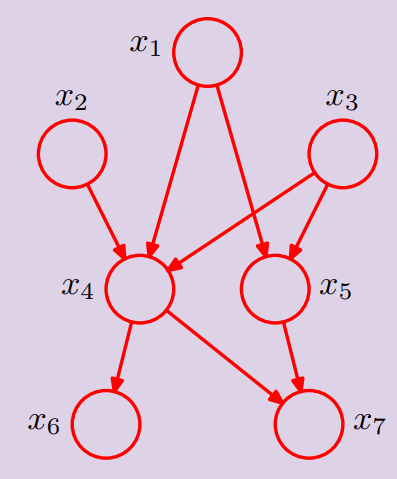
\includegraphics[width=0.5\textwidth]{images/bayesianNetworkExample.png}
    \caption{Bayesian Network example.}
    \label{fig:bayesianNetworkExample}
\end{figure}
The \textit{non-descendants} of a variable are the nodes which can not be reached following arrows from the variable. The subscript $l$ in $\mathcal{I}_l (\mathcal{G})$ stands for \textit{local} because, as discussed in the following, the model can also encode some global indipendences. \newline

Now we explain how to represent probabilistic relationships among a set of variables by means of a Bayesian Network.
\begin{itemize}
    \item Let $\mathcal{X}$ be a set of variables
    \item Let $p$ be a joint probability distribution over variables $\mathcal{X}$. Here we assume that $p$ is known, in practice we typically have to learn it from data
    \item Let $\mathcal{I}(p)$ be the set of independence assertions holding in $p$
    \item $\mathcal{G}$ is an \textit{independency map} (I-map) for $p$ if $p$ satisfies the local independences of $\mathcal{G}$:
    $$\mathcal{I}_l(\mathcal{G}) \subseteq \mathcal{I}(p)$$
    \textbf{Remark:} Note that given $\mathcal{I}_l(\mathcal{G}) \subseteq \mathcal{I}(p)$, the reverse is not necessarily true: there can be independences in $p$ that are not modelled by $\mathcal{G}$, perhaps we do not know them or the specific graphical model does not allow to encode them. Simmetrically, if we encode an independency in $\mathcal{G}$, this independecy should also hold in $p$.
\end{itemize}
Suppose we have to model a joint probability distribution $p(x_1, \hdots, x_m)$ among $m$ binary variables, we have to consider $2^m$ possible configurations which can soon become intractable. Our aim is to break down this joint probability into pieces. We say that $p$ \textit{factorizes} according to $\mathcal{G}$ if:
$$p(x_1, \hdots, x_m) = \prod_{i=1}^m p(x_i | \mathit{Pa}_{x_i})$$
where $\mathit{Pa}_{x_i}$ stands for the parents of $x_i$. Consider for example the Bayesian Network illustrated in Figure \ref{fig:bayesianNetworkExample}:
$$p(x_1, \hdots, x_7) = p(x_1)p(x_2)p(x_3)p(x_4|x_1,x_2,x_3)p(x_5|x_1,x_3)p(x_6|x_4)p(x_7|x_4,x_5)$$
Factorization is useful beacuse it breaks down a formula involving many variables into a product of formulas typically involving less values. In the example above, modeling $p(x_1,\hdots, x_7)$ as a single joint distribution, it would have required taking into consideration $2^7$ possible parameters (assuming only binary variables for simplicity), one for each possible configuration. On the other hand, the pieces on the left side of the equation involve significantly less paramaters:
\begin{itemize}
    \item $p(x_1),p(x_2),p(x_3)$ have 2 possible configurations
    \item $p(x_4|x_1,x_2,x_3)$ has $2^4$ possible configurations beacause it involves 4 variables
    \item $p(x_5|x_1,x_3), p(x_7|x_4,x_5)$ have $2^3$ possible configurations
    \item $p(x_6|x_4)$ has $2^4$ possible configurations
\end{itemize}
The order of complexity is around $2^4$ against $2^7$. \newline

This important result about factorization holds:
\begin{itemize}
    \item If $\mathcal{G}$ is an I-map for $p$, then $p$ factorizes according to $\mathcal{G}$
    \item If $p$ factorizes according to $\mathcal{G}$, then $\mathcal{G}$ is an I-map for $p$
\end{itemize}

The proof that this is the case follows: \newline

\textbf{I-map} $\Rightarrow$ \textbf{factorization}
\begin{enumerate}
    \item If $\mathcal{G}$ is an I-map for $p$, then $p$ satisfies (at least) these (local) independences:
    $$\{ \forall i \; x_i \perp \mathit{NonDescendants}_{x_i} | \mathit{Parents}_{x_i}\}$$
    
    \item Let us order variables in a \textit{topological order} relative to $\mathcal{G}$, i.e.:
    $$x_i \rightarrow x_j \Rightarrow i<j$$
    The variables in the Bayesian Network in Figure \ref{fig:bayesianNetworkExample} are already ordered topologically.
    
    \item Let us decompose the joint probability using the chain rule as:
    \begin{align*}
        p(x_1, \hdots, x_m) &= p(x_m | x_1, \hdots, x_{m-1})P(x_1,\hdots,x_{m-1})\\
        &= \prod_{i=1}^m p(x_i | x_1, \hdots, x_{i-1})
    \end{align*}
    
    \item Since nodes are topologically ordered, in $p(x_m | x_1, \hdots, x_{m-1})$ $x_m$ is conditioned on non-descendants. Local indipendences imply that for each $x_i$, in calculating $p(x_i | x_1, \hdots, x_{i-1})$, the only non-descendants $x_j \in \{x_1, \hdots, x_{i-1}\}$ which are relevant are the parents of $x_i$:
    $$p(x_i | x_1, \hdots, x_{i-1}) = p(x_i | \mathit{Pa}_{x_i})$$
\end{enumerate}

\textbf{factorization} $\Rightarrow$ \textbf{I-map}
\begin{enumerate}
    \item If $p$ factorizes according to $\mathcal{G}$, the joint probability can be written as:
    $$p(x_1, \hdots, x_m) = \prod_{i=1}^m p(x_i | \mathit{Pa}_{x_i})$$
    
    \item Let us consider the last variable $x_m$ (repeat steps for the other variables). By the product (chain) and sum rules:
    $$p(x_m|x_1, \hdots, x_{m-1}) = \frac{p(x_1, \hdots, x_{m})}{p(x_1, \hdots, x_{m-1})} = \frac{p(x_1, \hdots, x_{m})}{\sum_{x_m} p(x_1, \hdots, x_{m}))}$$
    
    \item Applying factorization and isolating the only term containing $x_m$ (the other terms which do not contain $m$ are constant with respect to the summation and can be taken out from the summation) we get:
    
    \begin{align*}
        \frac{p(x_1, \hdots, x_{m})}{\sum_{x_m} p(x_1, \hdots, x_{m}))} &= \frac{\prod_{i=1}^m p(x_i | \mathit{Pa}_{x_i})}{\sum_{x_m} \prod_{i=1}^m p(x_i | \mathit{Pa}_{x_i})} \\
        &= \frac{p(x_m | \mathit{Pa}_{x_m}) \cancel{\prod_{i=1}^{m-1} p(x_i|\mathit{Pa}_{x_i})}}{\cancel{\prod_{i=1}^{m-1} p(x_i | \mathit{Pa}_{x_i})} \cancel{\sum_{x_m}p(x_m | \mathit{Pa}_{x_m})}}
    \end{align*}
    
    \textbf{Remark:} $\sum_{x_m}p(x_m | \mathit{Pa}_{x_m})=1$ since we are summing over all possible values of $x_m$.\\
    \textbf{Remark:} In $p(x_m | x_1, \hdots, x_{m-1})$ all the variables in $\{x_1, \hdots, x_{m-1}\}$ are necessarily non-descendants of $x_m$ since we have defined a topological order.\\
    At the end of the day, we can conclude that the probability of $x_m$ given the non-descendants is equal to the probability of $x_m$ given the parents.
    
    \item If this property holds for $x_m$, for the same reasoning the property must holds for all the other variables. In other words, following this procedure we recover the set of independences that define an I-map.
\end{enumerate}

At this point we can conclude: factorization $\Leftrightarrow$ I-map.

\defi{\textbf{Bayesian Network} \label{def:bayesian_network}\\
A \textit{Bayesian Network} is a pair ($\mathcal{G}, p$) where $p$ factorizes over $\mathcal{G}$ (which is a Bayesian network structure) and it is represented as a set of conditional probability distributions (cpd) associated with the nodes of $\mathcal{G}$ ($p(x_1 | \mathit{Pa}_{x_1}), p(x_1 | \mathit{Pa}_{x_1}), \hdots, p(x_m | \mathit{Pa}_{x_m})$).

$$p(x_1, \hdots, x_m) = \prod_{i=1}^m p(x_i | \mathit{Pa}_{x_i})$$
}

\section{Example of Bayesian Network: toy regulatory network}
They are given three genes such that:
\begin{itemize}
    \item genes A and B have independent prior probabilities
    \item gene C can be enhanced by both A and B (if A and B are active, i.e. they are producing proteins, then it is more probable that also C is active)
\end{itemize}
We can represent this probabilistic setting with a Bayesian network as illustrated in Figure \ref{fig:geneBayesian}.
For the sake of simplicity, we assume that the variables are binary (active or inactive). In the context of binary variables, the conditional probability distribution becomes a conditional probability table, i.e. for each possible value of the variables there is a probability value.
According to the structure of the network, the joint probability decomposes as:
$$P(A,B,C) = P(C | A,B) P(A) P(B)$$
Since A and B have no parents, we simply build the two tables as follows:
\begin{center}
\begin{tabular}{c|c|c} 
 \hline
 gene & value & P(value)\\ 
 \hline
 A & active & 0.3\\ 
 A & inactive & 0.7
\end{tabular}
\end{center}

\begin{center}
\begin{tabular}{c|c|c} 
 \hline
 gene & value & P(value)\\ 
 \hline
 B & active & 0.3\\ 
 B & inactive & 0.7
\end{tabular}
\end{center}

On the other hand, mapping $P(C|A,B)$ is slightly more difficult. The conditional probability table has indeed 3 variables. The table is illustrated in Figure \ref{fig:geneBayesian_tableC}.\\
\textbf{Remark:} of course the columns of the conditional probability table proposed in Figure \ref{fig:geneBayesian_tableC} sum to one.

\begin{figure}
    \centering
    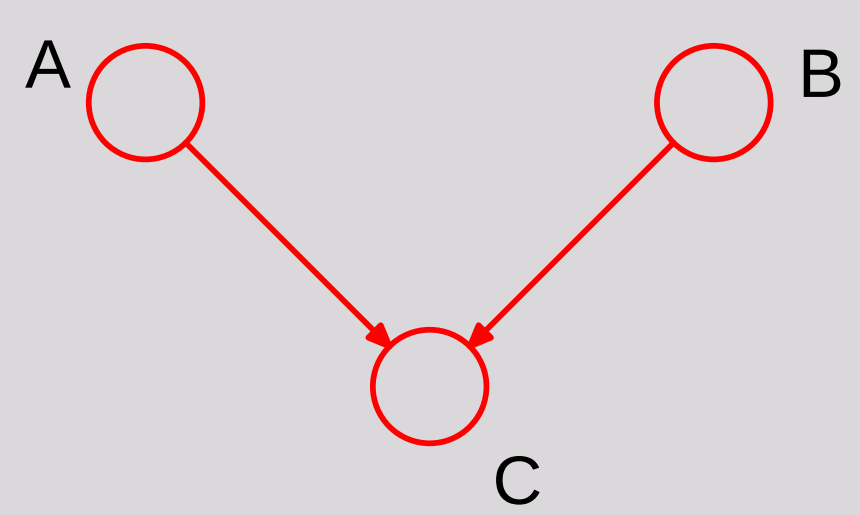
\includegraphics[width=0.5\textwidth]{images/geneBayesian.png}
    \caption{Toy regulatory network.}
    \label{fig:geneBayesian}
\end{figure}

\begin{figure}
    \centering
    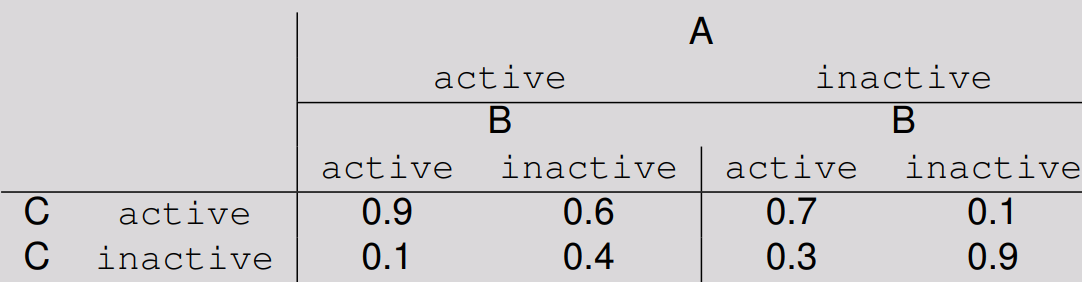
\includegraphics[width=\textwidth]{images/tabellaCGenes.png}
    \caption{Conditional probability table of gene C in the toy regulatory network proposed in Figure \ref{fig:geneBayesian}.}
    \label{fig:geneBayesian_tableC}
\end{figure}

\section{Conditional independence}
A graphical model is a way to make independences assumptions explicit in the structure of the model. \newline

Two variables $a,b$ are independent (written $a \perp b | \emptyset$) if:
\begin{equation}
    p(a,b) = p(a)p(b)
\end{equation}

Two variables $a,b$ are conditionally independent given $c$ (written $a \perp b | c$) if:
\begin{equation}
    \label{conditional_independence}
    p(a,b | c) = p(a|c) p(b|c)
\end{equation}

Independence assumptions can be verified by repeated applications of sum and product rules in order to see whether relations like \ref{conditional_independence} are actually true. However, doing these kind of mathematical derivations can become tedious. Whereas, with a graphical model which encodes the probability independences which we assume the distribution has, the procedure becomes simplier. Graphical models allow to directly verify independence assumptions through the \textit{d-separation} criterion.

\subsection{d-separation}
In order to introduce the process of d-separation, we start analyzing the base cases. The first relevant base case involves three variables. Indeed, the two variables case is trivial, since either the two variables are linked together and so they are related or there is no connection between the two variables and so they are not related. In a similar manner, also the case with three variables illustrated in Figure \ref{fig:trivialDSeparationThreeVariable} is trivial since each variable is related (i.e. there is a link) to the others. As a consequence everybody is dependent with respect to everybody else. There is nothing non-trivial to find out. The non-trivial case is when not all the three variables are connected to all the others (e.g. one link is missing). An example is illustrated in Figure \ref{fig:nonTrivialThreeVars}.

\begin{figure}
    \centering
    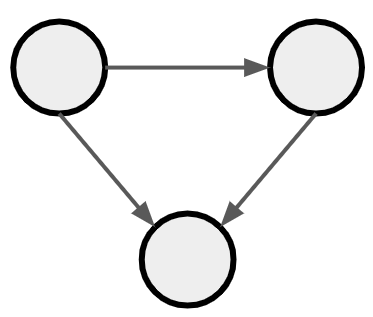
\includegraphics[width=0.5\textwidth]{images/exmpleTrivialThreeVariables.png}
    \caption{In this case although three variables are involved, verifying independency assumptions is trivial since each variable is related to the others.}
    \label{fig:trivialDSeparationThreeVariable}
\end{figure}

\begin{figure}
    \centering
    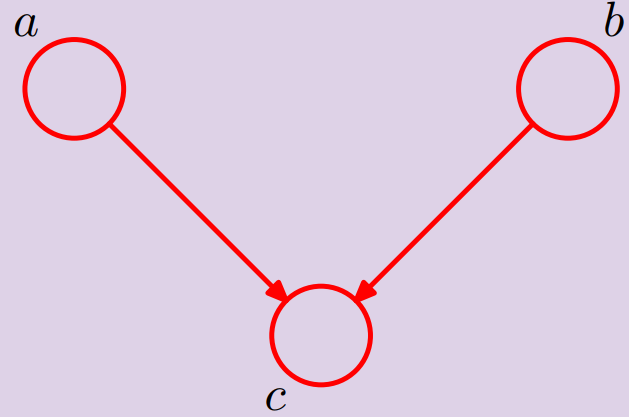
\includegraphics[width=0.5\textwidth]{images/nonTrivialThreeVars.png}
    \caption{In this case the independences among the three variables are not trivial.}
    \label{fig:nonTrivialThreeVars}
\end{figure}

In the following we discuss about the possible non trivial configurations of three variables. For consistency, we assume that the variable in the middle is identified with \textit{c}, while the variable on the left and the variable on the right are named \textit{a} and \textit{b} respectively.

\subsubsection{Tail-to-tail}
An example of this configuration is illustrated in Figure \ref{fig:tail-to-tail}.\\
The pattern is called \textit{tail-to-tail} because the central node \textit{c} is connected to the other variables by means of the tails of the two arrows.\\
Looking at the structure in Figure \ref{fig:tail-to-tail}, the joint probability distribution is:
$$p(a,b,c) = p(a|c)p(b|c)p(c)$$
At this point, our purpose is to understand whether $a$ and $b$ are independent ($a \perp b | \emptyset$) or not ($a \top\!\!\!\!\top b | \emptyset$). $a$ and $b$ are independent if:
$$p(a,b) = p(a)p(b)$$
Given $p(a,b,c)$ we get:
$$p(a,b) = \sum_c p(a,b,c)$$
According to the structure in Figure \ref{fig:tail-to-tail}, we can write:
$$p(a,b) = \sum_c p(a|c)p(b|c)p(c)$$

Actually, this formula does not simplify into $p(a)p(b)$:
$$p(a,b) = \sum_c p(a|c)p(b|c)p(c) \neq p(a)p(b)$$
as a result $a$ and $b$ are \textbf{not independent}. \newline
However, $a$ and $b$ are \textbf{conditionally independent given} $c$ (Figure \ref{fig:selectedTailToTail}):
\begin{equation*}
p(a,b|c) = \frac{p(a,b,c)}{p(c)} = \frac{p(a|c)p(b|c)p(c)}{p(c)} = p(a|c)p(b|c)
\end{equation*}

In other words, once $c$ is observed, $a$ and $b$ become independent. \newline

\textbf{Example 1:}
\begin{itemize}
    \item $a=$Bike
    \item $b=$Bus delay
    \item $c=$Rain
\end{itemize}

\textbf{Example 2:}
\begin{itemize}
    \item $a=$Cough
    \item $b=$Temperature
    \item $c=$Covid
\end{itemize}

\begin{figure}
\centering
\begin{subfigure}[t]{0.49\textwidth}
\centering
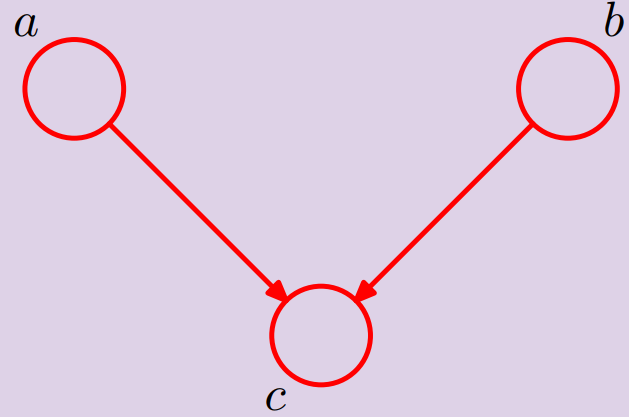
\includegraphics[width=\linewidth]{images/nonTrivialThreeVars.png} 
\caption{$a$ and $b$ are not independent.}
\label{fig:unSelectedTailToTail}
\end{subfigure}
\hfill
\begin{subfigure}[t]{0.49\textwidth}
\centering
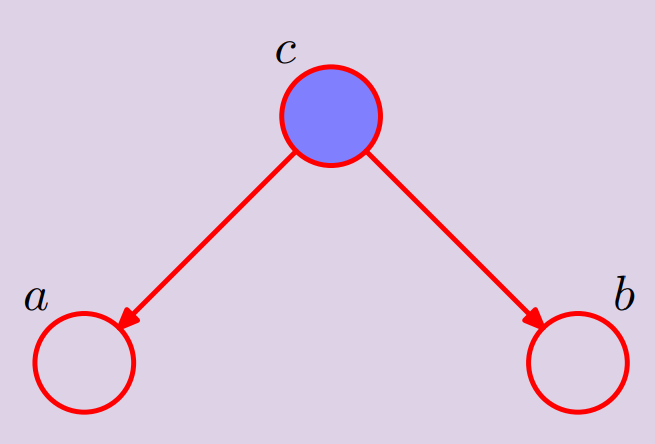
\includegraphics[width=\linewidth]{images/tailtToTailSelected.png}
\caption{$a$ and $b$ are conditionally independent given $c$.}
\label{fig:selectedTailToTail}
\end{subfigure}

\caption{Tail-to-tail}
\label{fig:tail-to-tail}
\end{figure}

\subsubsection{Head-to-tail}
In this case node $c$ is in the middle of a chain, Figure \ref{fig:head-to-tail}. Similarly to the previous case, this configuration is called \textit{head-to-tail} because variable $c$ is connected to $a$ and $b$ by means of the head of an arrow and a tail of another arrow. \newline

\textbf{Remark:} head-to-tail and tail-to-head are the same configuration because the labels $a$, $b$, $c$ are arbitrary. The only thing which matters is the chain that characterizes the structure. \newline

The joint probability $p(a,b,c)$ decomposes as follows:
$$p(a,b,c) = p(b|c)p(c|a)p(a)$$
We use this result to compute $p(a,b)$:
$$p(a,b) = \sum_c p(a,b,c) = p(a) \sum_c p(b|c)p(c|a)$$
There is no way applying probability rules to satisfy the equality $p(a) \sum_c p(b|c)p(c|a) = p(a)p(b)$. Given this, we can conclude that $a$ and $b$ are \textbf{not independent}:
$$p(a,b) = \sum_c p(b|c)p(c|a) \neq p(a)p(b)$$
On the other hand $a$ and $b$ are \textbf{conditionally independent given} $c$:
$$p(a,b | c) = \frac{p(a,b,c)}{p(c)} = \frac{p(b|c)p(c|a)p(a)}{p(c)}$$
Applying the Bayes rule we notice that:
$$\frac{p(c|a)p(a)}{p(c)} = p(a|c)$$
So:
$$p(a,b | c) = \frac{p(b|c)p(c|a)p(a)}{p(c)} = p(b|c)p(a|c)$$
Intuitively, if you have already observed the effects of a certain cause, you don't really care about the cause anymore in order to update the probability of the consequence. \newline

\textbf{Example:}
\begin{itemize}
    \item $a=$Cloudy
    \item $b=$Rainy
    \item $c=$Get wet
\end{itemize}
Assume that a student of the DISI department of the University of Trento named Giovanni Valer wakes up and notices that it's a cloudy day. He realizes that, if he goes to the university by bike, he could get wet. Indeed, since it is cloudy, it could rain. The fact that it is cloudy influences the chance of getting wet (causality reasoning).\\
Suppose not that Giovanni wakes up and it is raining but at the same time there is the sun. Even if it is not cloudy, Giovanni gets wet if he travels by bike to the university. Evidently, given that it is raining, the fact that it is not cloudy does not influence the probability of getting wet.

\begin{figure}
\centering
\begin{subfigure}[t]{0.49\textwidth}
\centering
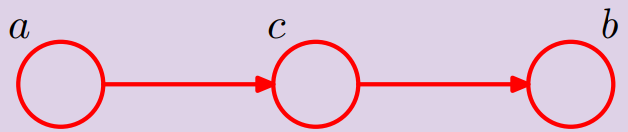
\includegraphics[width=\linewidth]{images/headToTail.png} 
\caption{$a$ and $b$ are not independent.}
\label{fig:unSelectedHeadToTail}
\end{subfigure}
\hfill
\begin{subfigure}[t]{0.49\textwidth}
\centering
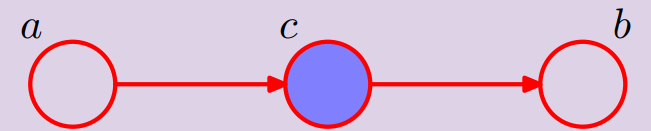
\includegraphics[width=\linewidth]{images/headToTailSelected.png}
\caption{$a$ and $b$ are conditionally independent given $c$.}
\label{fig:selectedHeadToTail}
\end{subfigure}

\caption{Head-to-tail}
\label{fig:head-to-tail}
\end{figure}

\subsubsection{Head-to-Head}
For the same reasons of the previous cases, the structure exemplified in Figure \ref{fig:head-to-head} is called \textit{head-to-head}. In this case the joint distribution decomposes as:
$$p(a,b,c) = p(c|a,b)p(a)p(b)$$
Calculating $p(a,b)$ summing over $c$ we notice that $p(a)$ and $p(b)$ can be extracted from the summation since they do not depend on $c$. Moreover, $\sum_c p(c|a,b) = 1$:
$$p(a,b) = \sum_c p(c|a,b) p(a) p(b) = p(a)p(b)$$

Therefore, we can conclude that $a$ and $b$ are \textbf{independent}. \newline

In this case we are not able to simplify $p(a,b|c)$ in order to verify the equality $p(a,b|c) = p(a|c)p(b|c)$. Actually, $a$ and $b$ are \textbf{not conditionally independent given} $c$:
$$p(a,b|c) = \frac{p(c|a,b)p(a)p(b)}{p(c)} \neq p(a|c)p(b|c)$$

Intuitively in this case $a$ and $b$ are competing causes of the effect $c$. At the beginning $a$ and $b$ are independent causes, but once the effect $c$ is observed they compete for the explanation. As a result, observing the result of one of them, reduces the probability of the other. This situation is usually referred to as \textit{explaining away effect}. \newline

\textbf{Example:}
\begin{itemize}
    \item $a=$Burglar
    \item $b=$Earthquake
    \item $c=$Alarm
\end{itemize}
Burglar and earthquake can be both possible causes for the alarm to ring. Of course, the burglar can decide to steal something from the house of Giovanni Valer regardless of the probability of an earthquake.\\
However, if the alarm rings Giovanni immediately thinks about a burglar. But if there is an earthquake in that moment, then the probability of a burglar in the mind of Giovanni decreases to 0.

\begin{figure}
\centering
\begin{subfigure}[t]{0.49\textwidth}
\centering
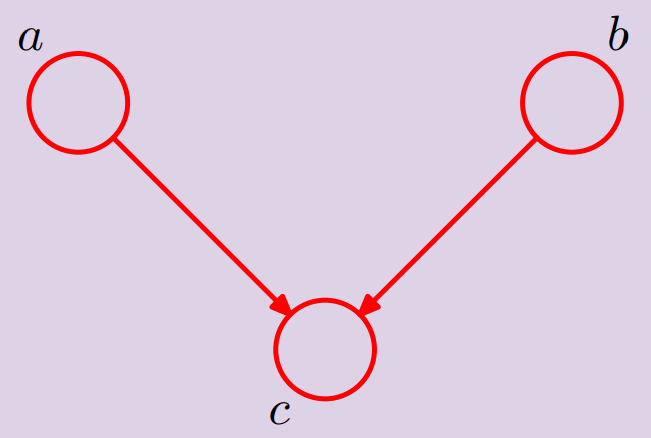
\includegraphics[width=\linewidth]{images/headToHead.png} 
\caption{$a$ and $b$ are independent.}
\label{fig:unSelectedHeadToHead}
\end{subfigure}
\hfill
\begin{subfigure}[t]{0.49\textwidth}
\centering
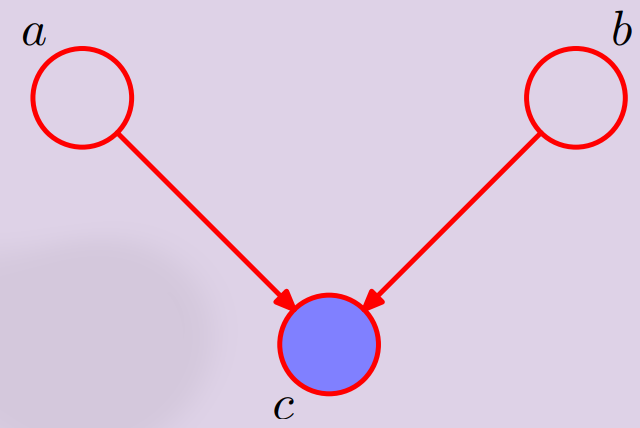
\includegraphics[width=\linewidth]{images/headToHeadSelected.png}
\caption{$a$ and $b$ are not conditionally independent given $c$.}
\label{fig:selectedHeadToHead}
\end{subfigure}

\caption{Head-to-head}
\label{fig:head-to-head}
\end{figure}

\begin{figure}
    \centering
    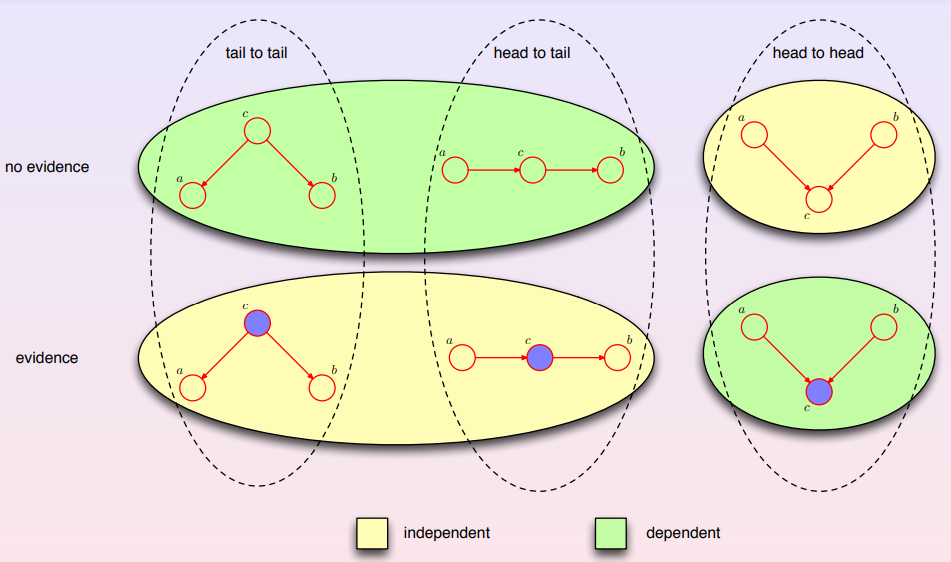
\includegraphics[width=\textwidth]{images/dSeparationSummary.png}
    \caption{d-separation: basic rules summary.}
    \label{fig:basicRulesSummary}
\end{figure}

\subsubsection{Example of head-to-head connection}
In this example we take into consideration a fuel system in a car. Our problem setting studies three random binary variables:
\begin{itemize}
    \item \textit{Battery}[B]: either charged (B=1) or flat (B=0)
    \item \textit{Fuel tank}[F]: either full (F=1) or empty (F=0)
    \item \textit{Electric fuel gauge}[G]: it indicates either full tank (G=1) or empty tank (G=0) 
\end{itemize}
The probabilistic dependences among these variables are represented by the Bayesian Network in Figure \ref{fig:fuelExample}. \newline

\textbf{Conditional probability tables (CPT)}
\begin{itemize}
    \item Battery and tank have independent prior probabilities:
    $$P(B=1) = 0.9$$
    $$P(F=1) = 0.9$$
    \item The fuel gauge is conditioned on both (unreliable):
    $$P(G=1 | B=1, F=1) = 0.8$$
    $$P(G=1 | B=0, F=1) = 0.2$$
    $$P(G=1 | B=1, F=0) = 0.2$$
    $$P(G=1 | B=0, F=0) = 0.1$$
\end{itemize}

\textbf{Probability reasoning} \newline

In this case the joint probability decomposes as follows:
$$P(F,G,B) = P(G | B,F)P(B)P(F)$$

Suppose that we are interesting in reasoning about the probability of empty tank.
\begin{itemize}
    \item The prior probability, without observing anything is:
    $$P(F=0) = 1 - P(F=1) = 0.1$$
    
    \item The posterior after observing empty fuel gauge (Figure \ref{fig:fuelExampleSelected}) is different:
    
    \begin{align*}
    P(F=0 | G=0) = \\
    &=\frac{P(G=0 | F=0) P(F=0)}{P(G=0)} =\\
    &=\frac{\sum_B [P(G=0,B | F=0)] P(F=0)}{P(G=0)} =\\
    &=\frac{\sum_B [P(G=0 | F=0, B) P(B|F=0)] P(F=0)}{P(G=0)}
    \end{align*}

    $F$ is not a descendant of $B$, as a result $P(B|F=0) = P(B)$. $B$ is independent with respect to its non descendants given the parents and $B$ has no parents.
    
    \begin{align*}
    P(F=0 | G=0) = \\
    &=\frac{\sum_B [P(G=0 | F=0, B) P(B|F=0)] P(F=0)}{P(G=0)} =\\
    &=\frac{\sum_B [P(G=0 | F=0, B) P(B)] P(F=0)}{P(G=0)}
    \end{align*}
    
    Now, we compute the denominator:
    \begin{align*}
    P(G=0) =\\
    &=\sum_{B \in \{0,1\}} \sum_{F \in \{0,1\}} P(G=0, B, F) =\\
    &= \sum_{B \in \{0,1\}} \sum_{F \in \{0,1\}} P(G=0 | B, F)P(B,F) = \\
    &= \sum_{B \in \{0,1\}} \sum_{F \in \{0,1\}} P(G=0 | B, F) P(F|B) P(B)
    \end{align*}
    Given the network, $F$ is independent with respect to its non descendants given its parents and $F$ has no parents.
    \begin{align*}
        P(G=0) =\\
        &= \sum_{B \in \{0,1\}} \sum_{F \in \{0,1\}} P(G=0 | B, F) P(F|B) P(B)\\
        &=\sum_{B \in \{0,1\}} \sum_{F \in \{0,1\}} P(G=0 | B, F)P(B)P(F)
    \end{align*}
    
    At the end of the day:
    \begin{align*}
    P(F=0 | G=0) =\\
    &=\frac{\sum_B [P(G=0 | F=0, B) P(B)] P(F=0)}{P(G=0)} =\\
    &=\frac{\sum_B [P(G=0 | F=0, B) P(B)] P(F=0)}{\sum_{B \in \{0,1\}} \sum_{F \in \{0,1\}} P(G=0 | B, F)P(B)P(F)} \simeq 0.257
    \end{align*}
    
\end{itemize}

The probability that the tank is empty increases from observing that the fuel gauge reads empty (not as much as expected because a strong prior and unreliable gauge). \newline

\textbf{Remark:} In real world applications, we typically observe the effects rather than the causes (e.g. we observe symptoms, not the pathology). We have to apply probability rules and in particular the Bayes theorem in order to reason about the probability of the causes. This is why this structures are named Bayesian Networks. \newline

\begin{figure}
\centering
\begin{subfigure}[t]{0.32\textwidth}
\centering
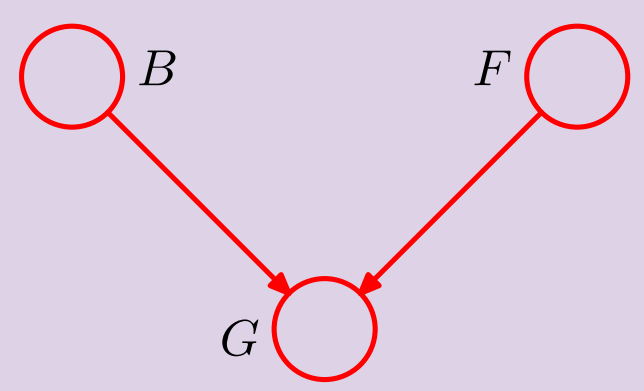
\includegraphics[width=\textwidth]{images/fuelExample.png}
\caption{Example of head-to-head connection.}
\label{fig:fuelExample}
\end{subfigure}
\hfill
\begin{subfigure}[t]{0.32\textwidth}
\centering
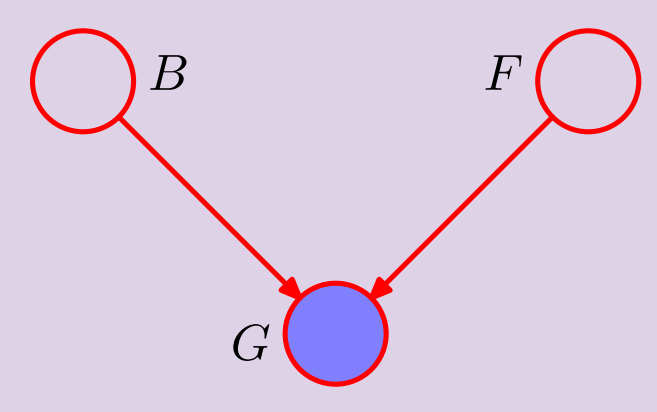
\includegraphics[width=\linewidth]{images/fuelExampleSelected.png}
\caption{The probability that the tank is empty increases from observing that the fuel
gauge reads empty.}
\label{fig:fuelExampleSelected}
\end{subfigure}
\hfill
\begin{subfigure}[t]{0.32\textwidth}
\centering
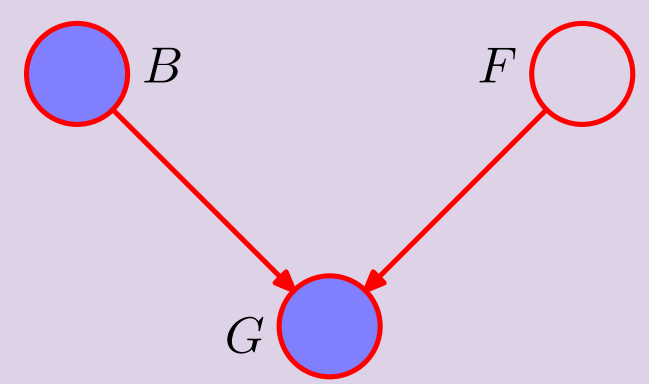
\includegraphics[width=\linewidth]{images/fuelExamplePart2.png}
\caption{The probability that the tank is empty decreases after observing that the battery is also flat.}
\label{fig:fuelExampleSelectedPart2}
\end{subfigure}

\caption{Head-to-head}
\label{fig:head-to-head-example}
\end{figure}

Suppose that now, we are interesting in the posterior probability after observing that the battery is also flat (Figure \ref{fig:fuelExampleSelectedPart2}).

\begin{align*}
P(F=0 | G=0, B=0) = \\
&=\frac{P(G=0|F=0,B=0)P(F=0|B=0)}{P(G=0|B=0) \simeq 0.111}
\end{align*}

From this we understand that $F$ and $B$ are related once $G$ is known. If they were unrelated, knowing something about $B$ would not change the probability value. On the contrary, the probability that the tank is empty decreases after observing that the battery is also flat. The battery condition \textit{explains away} the observation that the fuel gauge reads empty. The probability is sill greater than the prior one, because the fuel gauge observation still gives some evidence in favour of an empty tank.

\subsubsection{d-separation in networks with more than three variables}
Naturally, it is interesting to study more complex configurations involving more than three random variables. \newline

\textbf{General Head-to-head}
\begin{itemize}
    \item Let a descendant of a node $x$ be any node which can be reached from $x$ with a path following the direction of the arrows.
    \item A head-to-head node $c$ unblocks the dependency path between its parents if either itself or any of its descendants receives evidence.
\end{itemize}

Consider the example in Figure \ref{fig:generalHeadToHead1}. As we explained above, $A$ and $B$ are independent in principle. However, once $C$ receives evidence, then $A$ and $B$ are dependent one with respect to the other. Analogously, in Figure \ref{fig:generalHeadToHead2} variables $A$ and $B$ are initially independent, but when $D$, which is a child of $C$, is observed, then $A$ and $B$ becomes mutually dependent. For instance, the four variables could represent the following events:
\begin{itemize}
    \item $A=$ burglar
    \item $B=$ earthquake
    \item $C=$ alarm
    \item $D=$ phone call from the alarm company
\end{itemize}
If Giovanni Valer is not at home but he receives a phone call from the alarm company he immediately thinks about a burglar even if he does not hear the alarm. Evidently, burglar and earthquake both compete for an indirect effect. \newline

This rules is valid for every descendant, though probably the further the descendant the less influent is the indirect connection.

\begin{figure}
\centering
\begin{subfigure}[t]{0.49\textwidth}
\centering
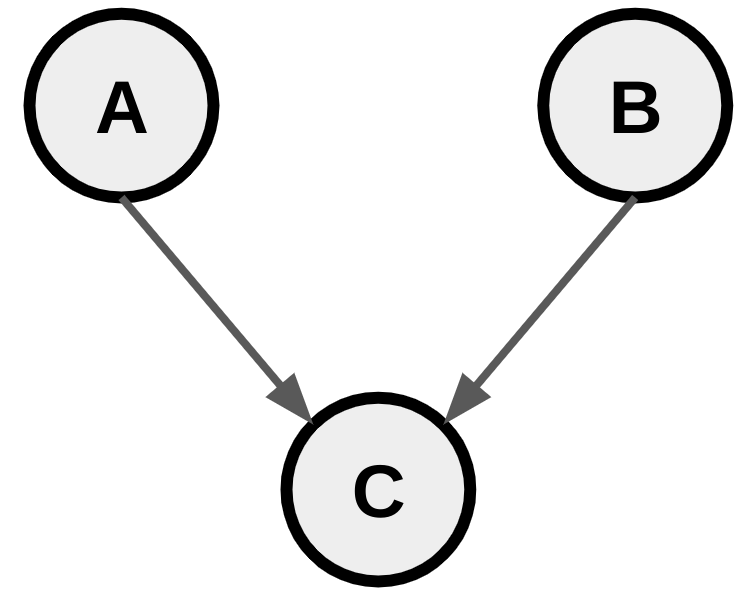
\includegraphics[width=\textwidth]{images/generalHeadToHead1.png}
\caption{Head-to-head connection among three random variables.}
\label{fig:generalHeadToHead1}
\end{subfigure}
\hfill
\begin{subfigure}[t]{0.49\textwidth}
\centering
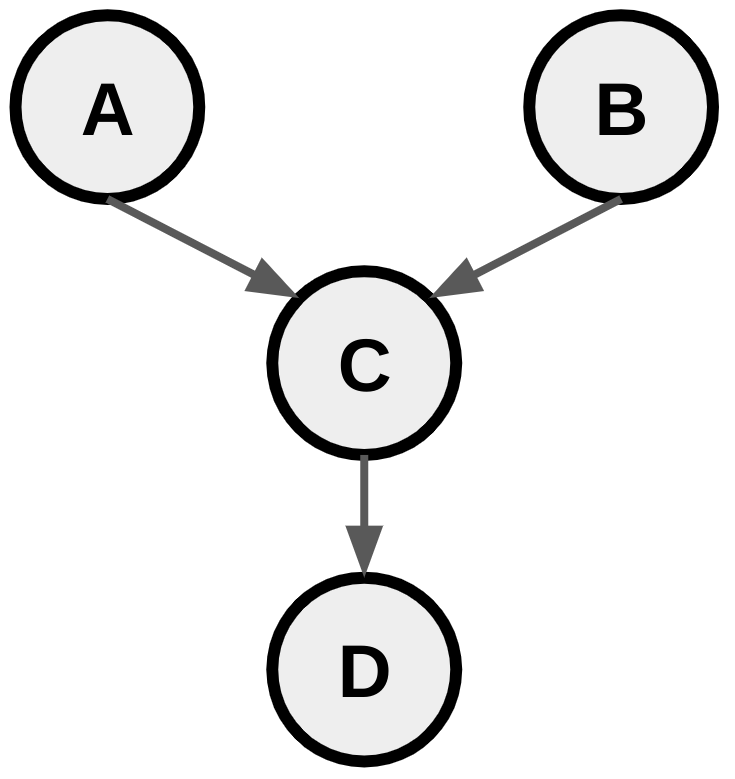
\includegraphics[width=\linewidth]{images/generalHeadToHead2.png}
\caption{Head-to-head connection among more than three random variables.}
\label{fig:generalHeadToHead2}
\end{subfigure}

\caption{General Head-to-head}
\label{fig:generalHeadToHead}
\end{figure}

\subsubsection{General d-separation criterion}
Given a generic Bayesian network. Given $A,B,C$ arbitrary nonintersecting sets of nodes. The sets $A$ and $B$ are \textit{d-separated} by $C$ ($\mathit{dsep}(A;B|C)$) if all paths from any node in $A$ to any node in $B$ are \textit{blocked} (there is no information flow along the path). Actually, if there is no information flow between $A$ and $B$, then $A$ and $B$ are independent given $C$.\\
A path is blocked if it includes at least one node s.t. either:
\begin{itemize}
    \item the arrows on the path meet tail-to tail (Figure \ref{fig:selectedTailToTail}) or head-to-tail (Figure \ref{fig:selectedHeadToTail}) at the node and it is in $C$, or
    \item the arrows on the path meet head-to-head at the node and neither it nor any of its descendants is in $C$ (Figure \ref{fig:selectedHeadToHead}).
\end{itemize}

\defi{\textbf{d-separation implies conditional independence} \label{def:d-separation}\\
The sets $A$ and $B$ are independent given $C$ ($A \perp B | C$) if they are d-separated by $C$.
}

In a sense, we are using the basic rules in Figure \ref{fig:basicRulesSummary} as building blocks to define the more general d-separation principle. The basic rules allow to understand if individual paths are blocked somewhere. It is sufficient that a path is blocked in one place to be completely blocked. \newline

\textbf{Example of general d-separation 1}

In this second example we consider the Bayesian Network in Figure \ref{fig:exampleDSeparation1}. In this case nodes $a$ and $b$ are not d-separated by $c$:
\begin{itemize}
    \item Node $f$ is tail-to-tail and not observed.
    \item Node $e$ is head-to-head and its child $c$ is observed.
\end{itemize}

We can conclude that $a \top\!\!\!\!\top b | c$. In other words, there is information flow from $a$ to $b$. \newline

\begin{figure}
    \centering
    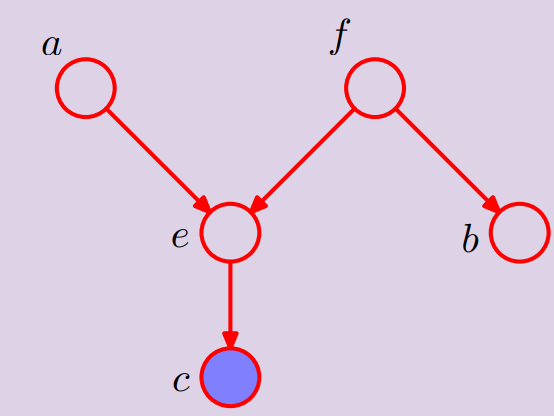
\includegraphics[width=0.5\textwidth]{images/exampleGeneralDSeparation1.png}
    \caption{Example of general d-separation. $a \top\!\!\!\!\top b | c$ }
    \label{fig:exampleDSeparation1}
\end{figure}

\textbf{Example of general d-separation 2} \newline
In this second example we consider the Bayesian Network in Figure \ref{fig:exampleDSeparation1.1}. In this case $a$ and $b$ are d-separated by $e$:
\begin{itemize}
    \item $e$ is head-to-head connected.
    \item $e$ is not observed.
    \item no children of $e$ are observed.
\end{itemize}

As a result there is no information flow via $e$. We can conclude that $\mathit{dsep}(A,B | \emptyset)$. \newline

\begin{figure}
    \centering
    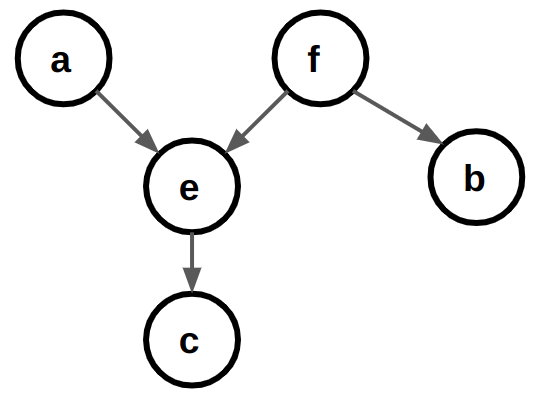
\includegraphics[width=0.5\textwidth]{images/exampleGeneralDSeparation1.1.png}
    \caption{Example of general d-separation. $a \perp b | c$ }
    \label{fig:exampleDSeparation1.1}
\end{figure}

\textbf{Example of general d-separation 3}

In this third example we consider the Bayesian Network in Figure \ref{fig:exampleDSeparation2}. In this case $a$ and $b$ are d-separated by $f$:
\begin{itemize}
    \item Node $f$ is tail-to-tail and observed.
\end{itemize}

In this case node $f$ blocks the flow of information. We can conclude that $a \perp b | f$. Intuitively, $a$ and $f$ are two possible causes for $b$. If $f$ is observed than the cause is already known. \newline

\begin{figure}
    \centering
    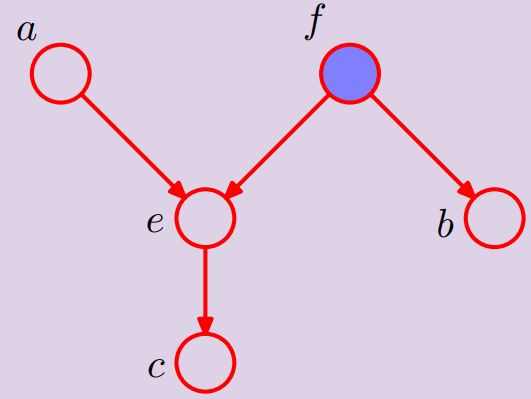
\includegraphics[width=0.5\textwidth]{images/exampleGeneralDSeparation2.png}
    \caption{Example of general d-separation. $a \perp b | c$ }
    \label{fig:exampleDSeparation2}
\end{figure}

\textbf{Example of general d-separation 4} \newline
In this fourth example, we consider the network in Figure \ref{fig:exampleDSeparation4} and we investigate if $A$ and $B$ are d-separated or not ($\mathit{dsep}(A,B|C)$). In order to answer to this question we have to examine all the possible paths between $A$ and $B$. In correspondence of $\alpha$ there is a head-to-head connection and node $\alpha$ is observed. Hence, we can conclude that information flows from $A$ to $B$ and the statement $\mathit{dsep}(A,B|C)$ is not true. \newline

\begin{figure}
    \centering
    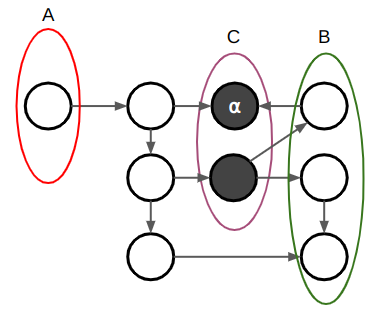
\includegraphics[width=0.5\textwidth]{images/exampleGeneralDSeparation3.png}
    \caption{Example of general d-separation. $A \top\!\!\!\!\top B | C$ }
    \label{fig:exampleDSeparation4}
\end{figure}

\textbf{Example of general d-separation 5} \newline
In this fifth example, we consider the network illustrate in Figure \ref{fig:exampleDSeparation5}. In this case the path 1-2-3-4 is blocked because in correspondence of node 3 there is a head-to-head connection but node 3 is not observed and it has no children. As a consequence we have to check other paths in order to understand whether or not $\mathit{dsep}(A,B|C)$. Moreover also paths 1-2-5-$\beta$-6 and 1-2-5-$\beta$-4 are blocked. However, along the chain 1-2-5-7-8 there are no observations. So along 1-2-5-7-8 information flows. We can conclude that $A$ and $B$ are not d-separated. \newline

\begin{figure}
    \centering
    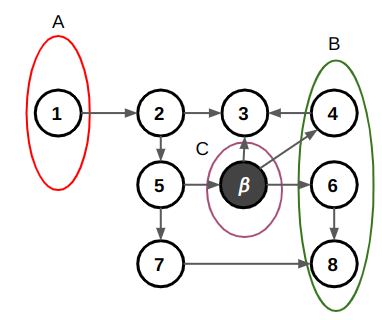
\includegraphics[width=0.5\textwidth]{images/exampleGeneralDSeparation4.png}
    \caption{Example of general d-separation. $A \top\!\!\!\!\top B | C$ }
    \label{fig:exampleDSeparation5}
\end{figure}

\textbf{Example of general d-separation 6} \newline
In this sixth example we consider the network illustrated in Figure \ref{fig:exampleDSeparation6}. Following the same reason as before, we understand that $A$ and $B$ are d-separated by $C$ this time.

\begin{figure}
    \centering
    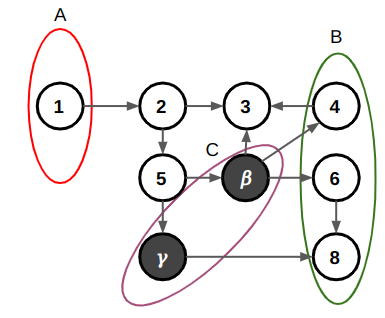
\includegraphics[width=0.5\textwidth]{images/exampleGeneralDSeparation5.png}
    \caption{Example of general d-separation. $A \perp B | C$ }
    \label{fig:exampleDSeparation6}
\end{figure}

\subsection{BN independences revisited}
\begin{itemize}
    \item A BN structure $\mathcal{G}$ encodes a set of \textit{local} independence assumptions:
    $$I_l(\mathcal{G}) = \{\forall i x_i \perp \mathit{NonDescendants}_{x_i}|\mathit{Parents}_{x_i}\}$$
    
    \item A BN structure $\mathcal{G}$ encodes a set of \textit{global} (Markov) independence assumptions:
    $$I(\mathcal{G}) = \{(A \perp B | C) : \mathit{dsep}(A;B|C)\}$$
\end{itemize}

\subsection{BN equivalence classes}
Quite different BN structures can actually encode the exact same set of independence assumptions. For example the three BNs in Figure \ref{fig:exampleIEquivalentBN} constitutes an equivalence class whose components encode the same independence assumptions. Figure \ref{fig:exampleIEquivalentBN2} represents the second independence class which encodes the opposite ($A$ and $B$ are not independent, they become independent when $C$ is observed) of the structures in Figure \ref{fig:exampleIEquivalentBN}. This concept can be generalized to arbitrary Bayesian Networks with more than three nodes. In general two BN structures (of course they have to be on the same set of nodes) $\mathcal{G}$ and $\mathcal{G}'$ are \textit{I-equivalent} if $I(G)=I(\mathcal{G}')$. Following this relation, the space of BN structures over $\mathcal{X}$ is partitioned into a set of mutually exclusive and exhaustive \textit{I-equivalence classes}.

\begin{figure}
\centering
\begin{subfigure}[t]{0.49\textwidth}
\centering
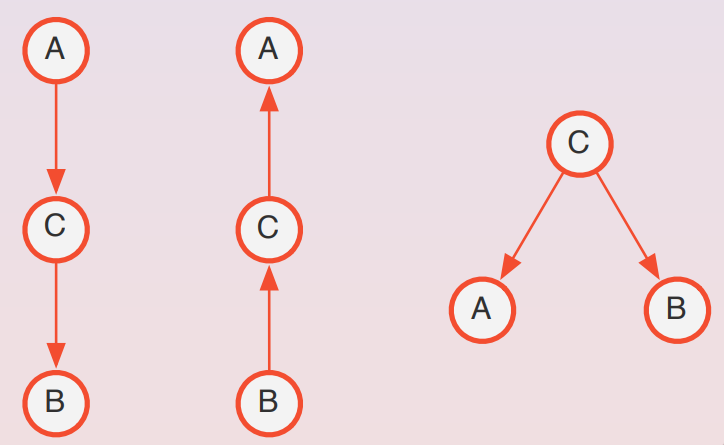
\includegraphics[width=\textwidth]{images/exampleIEquivalentBN.png}
\caption{The three BNs constitutes an equivalence class whose components encode the same independence assumptions.}
\label{fig:exampleIEquivalentBN}
\end{subfigure}
\hfill
\begin{subfigure}[t]{0.49\textwidth}
\centering
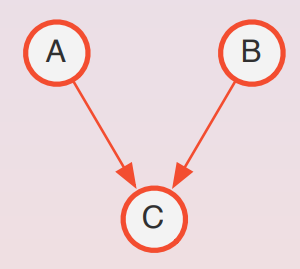
\includegraphics[width=0.7\linewidth]{images/exampleIEquivalentBN2.png}
\caption{A second independence class which encodes the opposite ($A$ and $B$ are not independent, they become independent when $C$ is observed) of the structures in Figure \ref{fig:exampleIEquivalentBN}.}

\label{fig:exampleIEquivalentBN2}
\end{subfigure}

\caption{BN equivalence classes}
\label{fig:BNequivalenceclasses}
\end{figure}

\section{I-maps vs distributions}
As explained above, for a structure $\mathcal{G}$ to be an I-map for $p$, it does not need to encode all its independences. As a consequence a fully connected graph is an I-map of any $p$i defined over its variables. Indeed, a fully connected graph does not encode any independency and so, for sure it does not encode an independency which is not in $p$. Obviously, a fully connected graph is not useful for our purposes.

\defi{\textbf{Minimal I-map} \label{def:minimalIMap}\\
A \textit{minimal I-map} for $p$ is an I-map $\mathcal{G}$ which can't be "reduced" into a $\mathcal{G}' \subset \mathcal{G}$ (by removing edges) that is also an I-map for $p$. In other words it is no more possible to remove edges from $\mathcal{G}$ without introducing independences which do not hold in $p$.
}

\textbf{Remark:} a minimal I-map for $p$ does not necessarily capture all the independences in $p$.

\defi{\textbf{Perfect Maps (P-maps)} \label{def:perfectMap}\\
A structure $\mathcal{G}$ is a \textit{perfect map} (P-map) for $p$ it captures all (and only) its independences:
$$I(\mathcal{G}) = I(p)$$
}

\textbf{Remark:} not all distributions have a P-map. Some cannot be modelled exactly by the BN formalism. In particular there are some independences which cannot be modelled by directed edges. \newline

There exists an algorithm for finding a P-map of a distribution which is exponential in the in-degree of the P-map. The algorithm returns an equivalence class of structures which are a perfect map rather than a single structure.

\section{Practical suggestions for building a Bayesian Network}
\label{sec::practicalSuggestions}
\begin{itemize}
    \item Get together with a domain expert.
    
    \item Define variables for entities that can be \textit{observed} (e.g. symptoms, age, weight) or that you can be interested in \textit{predicting} (e.g. pathology). Latent variables can also be sometimes useful. Latent variables are variables which we do not observe and we do not want to predict. However, they are mediators for what we need to predict. For instance, a certain pathology could depend on some groups of behaviours which could facilitate the prediction of the pathology.
    
    \item Try following \textit{causality} considerations in adding edges (edges which encode causalities are more interpretable and they tend to produce sparser networks).
    
    \item In defining probabilities for configurations (almost) never assign zero probabilities. Otherwise, every example with that configuration which we will observe in the future will have zero probability.
    
    \item It is usually difficult in real world applications to assign probabilities to certain variables configurations. As a result we typically refine or estimates these parameters using data. If data are available, use them to help in \textit{learning} parameters and structure of the network.
\end{itemize}
    \chapter{Inference in BN}
\label{cha:inter_BN}

The criteria with which a Bayesian Network (Chapter \ref{cha:bay_net}) is built, allows us to get information about the data.\\

We assume that we have evidence $e$ (what I observe) on the state of a subset of variables $E$ in the model. Therefore Inference amounts as computing the posterior probability of a subset $X$ of the non-observed variables given the observation:
$$P(X|E = e)$$
Inference is computing the probability of variable $X$ (one of more non-observed variables) given the observed variables (posterior probability of $X$ given the evidences).\\

A graphical model is designed as a network of joint probability, we can use messages to compute joint probability of the variable of interest and the evidence. Typically I need the conditional probability, then I need to compute (Bayes' theorem \ref{theo:bayes}):
$$P(X | E = e) = \frac{P(X, E=e)}{P(E=e)}$$
Then I need to compute $P(X, E=e)$ and $P(E=e)$, the denominator is easy (once I compute the numerator $P(E=e) = \sum_{X} P(X, E=e)$ (through a marginalization)), therefore I need to compute the nominator.\\
The nominator is a joint probability, I want to exploit the BN structure to compute this numerator easily, otherwise it will explode exponentially.
For this reason, we can exploit the structure of the Bayesian Network to get inference more easily, this will end up in a problem that can be solved using dynamic programming.

\section{Inference in chain-like structure}
    Let's start from a linear chain of nodes, which will be our BN (Bayesian Network).
    \begin{figure}[H]
        \centering
        \includegraphics[scale=0.3]{images/chain_inference_bn.png}
    \end{figure}
    We want to compute the probability for a certain node given some evidence:
    $$P(X| E=e) = \frac{P(X, E=e)}{P(E=e)}$$
    
    \subsection{Inference without evidence}
        Let's ignore the evidence first, then come back to that later.
        The probability of any of the nodes depends on the previous nodes as
        The joint distribution modelled on the BN is $P(X_1, \dots, X_n)$, then if I am interested in $P(X_n)$ I know that it possibly depends on all the other possible variables (marginalization)
        This is where the exponential problem would come up. 
        $$P(X_n) = \sum_{X_i \neq X_n} P(X_1, \dots, X_n)$$ 
        Considering joint probability decomposed according to the chain is
        $$P(X_n) = \sum_{X_1} \sum_{X_2} \dots \sum_{X_{n-1}} \sum_{X_{n+1}} \sum_{X_n} P(X_1)P(X_2|X_1)P(X_3|X_2)\dots P(X_n|X_{n-1})$$
        But we notice that the sum over $X_n$ has only a value in the decomposition which depends on it ($P(X_n|X_{n-1})$), the other probabilities are constant with respect to $X_n$. Therefore we represent this value as a function depending on $X_{n-1}$
        $$\mu_\beta (X_{n-1}) = \sum _{X_n} P(X_n|X_{n-1})$$
        So we get
        $$P(X_N) = \sum_{X_1} \sum_{X_2} \dots \sum_{X_{n-1}} P(X_1)P(X_2|X_1)P(X_3|X_2)\dots P(X_{n-1}|X_{n-2}) \mu_\beta (X_{n-1})$$
        We can proceed with the same intuition for all the previous members
        $$\mu_\beta (X_{i}) = \sum_{i+1} P(X_{i+1}|X_i)\mu_\beta(X_{i+1})$$
        I go back with this procedure until $n+1$.\\
        
        We can compute a similar procedure from the top to the bottom of the chain. Given
        $$P(X_n) = \sum_{X_1} \sum_{X_2} \dots \sum_{X_{n-1}} P(X_1)P(X_2|X_1)P(X_3|X_2)\dots P(X_n|X_{n-1})$$ 
        notice that the terms that depend on the first summation $\sum_{X_1}$ are only $P(X_1)P(X_2|X_1)$, then we can carry on the same reasoning
        $$\mu_\alpha (X_{2}) = \sum _{X_1} P(X_1)P(X_2|X_{1})$$
        where $\alpha$ stands for forward messages while $\beta$ for reverse messages.
        $$\sum_{X_2}\sum_{X_2}\dots \sum_{X_{n-1}} \mu_{\alpha}(X_2) P(X_3|X_2) \dots P(X_{n}|X_{n-1})$$
        In general: 
        $$\mu_\alpha (X_{i}) = \sum _{X_{i-1}} \mu_\alpha(X_{i-1}) P(X_i|X_{i-1})$$
        For the forward message we can stop when
        $$\mu_\alpha (X_{n}) = \sum_{X_{n-1}} \mu_\alpha (X_{n-1}) P(X_n|X_{n-1})$$
        The only term that is left from the two chain is $P(X_n)$ that can be written as
        $$P(X_n) = \mu_\alpha (X_n) \mu_\beta(X_n)$$
        this means that computing the local probabilities and summing them independently, using (for a binary problem) a number of operation equal to $2(n-1)$ instead of $2^n$. $\mu_\alpha$ and $\mu_\beta$ are message sent backwards or forward from node to node. 
        The message is always a function of the destination node: I am interested in computing the probability of the $i^{th}$ node and I collect the messages coming from the adjacent nodes.
        \begin{figure}[h]
            \centering
            \includegraphics[scale=0.3]{images/chain_inference_message_passing.png}
            \caption{Inference for the $i^{th}$ node based on the messages from the previous and next node passing}
            \label{fig:message_passing_inference_BN_chain}
        \end{figure}
        Nodes compute messages to be sent to the next node, as generalization, the message computed is a combination of a local probability of that node and the message received from the previous (or next) nodes: this is a standard way to send messages also for non-chain structures.\\
        
        It is clever to store the partial computations we can do the \textit{full message passing}: sending a message from the top to the end of the chain and vice versa, so we have already computed all the partial computation that we could need.\\
    
    \subsection{Inference adding evidence}
        Typically we have some observed values, and then we want to compute the probability: instead of the sum over the values for the variable that I observed we can plug in the value I actually observed.\\
        Let's say I observed $X_1 = x_{e1}, X_3 = x_{e3}$ in a chain of 4 elements and I what to compute $X_2$. This can be done as
        $$P(X_2|X_3 = x_{e3}, X_1 = x_{e1}) = \frac{P(X_1, X_2, X_3, X_4)}{P(X_3 = x_{e3}, X_1 = x_{e1})}$$
        the joint probability can be computed as
        $$\sum_{X_4} P(X_1, X_2, X_3, X_4) = P(X_1 = x_{e1}, X_2, X_3 = x_{e3}, X_4)$$ where for the observed values I can plug in the values
        $$\sum_{X_4} P(X_1 = x_{e1})P(X_2|X_3 = x_{e3}, X_1 = x_{e1})P(X_3 = x_{e3}))P(X_4|X_3 = x_{e3})$$
        The only term that depends of $X_4$ is the last probability, therefore
        $$\sum_{X_4} P(X_4|X_3 = x_{e3}) = \mu_\beta(X_3 = x_{e3})$$
        and for the latter I do have the value observed. 
        The inference procedure is actually the same, having evidence implies plugging in values instead of computing a summation.\\
        
        After all it is true that:
        \begin{equation}
            P(X_n|\textbf{X}_e = \textbf{x}_{e}) = \frac{P(X_n, \textbf{X}_e = \textbf{x}_{e})}{\sum_{X_n} P(X_n, \textbf{X}_e = \textbf{x}_e)}
        \end{equation}
        with bold values as evidence.
        
\section{Inference in trees-like structure}
    The solution highlighted for chains can be extended to trees. At this point we should consider different kind of structures:
    \begin{figure}
        \centering
        \includegraphics[scale=0.3]{images/trees_inferences.png}
        \caption{a) undirected trees b) directed trees c) directed poly-trees}
        \label{fig:trees_structure}
    \end{figure}
    
    \begin{enumerate}[label=(\alph*)]
        \item \textbf{undirected trees}: undirected graph with a single path for each pair of nodes
        \item \textbf{directed trees}: directed graph with a single node (root) with no parents, all other nodes with a single parent
        \item \textbf{directed poly-trees}: directed graphs with multiple parents, for node and multiple roots but still a single (undirected) path between each pair of nodes.
    \end{enumerate}
    
    The procedure that we will described will work for directed (BN) and undirected models (Markov's Models, \textit{MM}).\\
    
    In order to facilitate the description (and the implementation) we need to go through an alternative representation of the graphical model: a \textit{factor graph}. 
    \defi{\textbf{Factor graph}\label{def:factor_graph}\\
    It is a graphical representation of a graphical model highlighting its factorization. The factor graph is an undirected graph that has one node for each node in the original graph and also additional nodes for each factor (a factor node had undirected links to each of the node variables in the factor).
    }
    \begin{figure}[h]
        \centering
        \includegraphics[scale=0.3]{images/factor_graph.png}
        \caption{Example of two different factor graphs for the first directed graph.}
        \label{fig:factor_graph}
    \end{figure}
    A factor is a component of the joint distribution we are trying to represent. The value associated to the factor is a probability distribution.
    In Figure \ref{fig:factor_graph} we can look at two different realization of factor graphs for the easy directed graph on the left. The factor graph in the middle represent the following factorialization: \\
    $f(x_1, x_2, x_3) = p(x_3|x_1, x_2)P(x_1)P(x_2)$\\
    while the most right one stands for \\
    $f_a(x_1) = P(x_1)$\\
    $f_b(x_2) = P(x_2)$\\
    $f_c(x_1, x_2, x_3) = p(x_3|x_1, x_2)$\\
    This last one means that \\
    $P(x_1, x_2, x_3) = f_c(x_1, x_2, x_3)f_a(x_1)f_b(x_2)$\\
    The latter is the one that we will use ad default option since is the most complete.
    
    \subsection{The sum-product algorithm}
        If we think of the inference algorithm on chain, we took the incoming message, multiply over the local probability, summing over one variable and sending the message to another variable (\textit{sum-product alternation}): this procedure is efficient for tree-like structure (also chain as edge case).\\
        On factor graphs it still can be applied if the factor graph it belongs to one of the classes described in Figure \ref{fig:trees_structure} (a factor graph will not be directed).
        
        \subsubsection{Inference without evidence}
            At this point I have no evidence, and no sequence. I have a generic joint probability (marginalize on everything except $X$ in which I am interested)
            $$P(X) = \sum_{\textbf{X} \neq X} p(\textbf{X})$$
            Let us remind that in the chain case
            $$P(X_n) = \mu_\alpha (X_n) \mu_\beta(X_n)$$
            This version is the same but generalized to all the messages reaching the node (incoming), the node are only connected to factors (not nodes) therefore it is the product for all factors in the neighbourhood from the factor to $X$
            $$P(X) = \prod _{f_s \in adj(X)} \mu_{f_s \rightarrow X}$$
            where $f_s \rightarrow X$ stand for $f_s$ as source and $X$ as destination. The message is always a function of the variable \textit{node} because the factor has more variables.
            \begin{figure}[ht]
                \centering
                \includegraphics[scale=0.3]{images/message_BN_fwd.png}
                \caption{Collecting messages from the adjacent nodes of X (fwd message passing)}
                \label{fig:message_BN_fwd}
            \end{figure}
            The value corresponding to the message that $f_s \rightarrow X$ is the multiplication of the incoming messages from its adjacent nodes multiplied by the local probability of the factor.
            $$\mu_{f_s \rightarrow X} = \sum_{X_1}\dots\sum_{X_{m}} f(X, X_1, \dots, X_m) \prod _{X_i \in adj(f_s) \neq X} \mu_{X_i \rightarrow f_s}$$
            with $x_1, \dots, x_m$ the nodes that $f_s$ receives messages from (but the destination $X$).\\
            
            Computing the message from the node to a factor becomes simple: 
            I have a node that needs to send a message to a factor, then it will be connected only to factors node $f_1, \dots, f_n$. The message from $f \rightarrow X$ is always a function of the variable node, then we
            \begin{itemize}
                \item collect messages from the adjacent nodes, therefore multiply for all factors that are not the destination (this is the \textbf{product of the incoming messages} for all neighbours)
                $$\mu _ {X \rightarrow f} (X) = \prod _{f_i \in adj(X) \neq X} \mu _{f_i \rightarrow X} (X)$$
                \item if the messages is at the extremes, then we need to take care of leaves. We start sending messages from the leaves $X$, then the message will be equal to one since it has no incoming messages
                $$\mu _{X \rightarrow f}(X) = 1$$
                \item if the extreme is a factor, then we will not have any incoming messages and from this
                $$\mu_{f \rightarrow X} = \sum_{X_1}\dots\sum_{X_{m}} f(X, X_1, \dots, X_m) \prod _{X_i \in adj(f) \neq X} \mu_{X_i \rightarrow f}$$
                we get that it is only function of one variables
                $$\mu_{f \rightarrow X} = f(X)$$
            \end{itemize}
            We can start sending messages like this, and then things come together as sums and products.\\
            
            The message computation in a tree structure gets more complicated than a chain (in which it is enough to start from top and end of the chain). Given a tree, we have a root already defined, but in the factor graph we do not.\\
            Therefore we take one node (whatever) and use it as a root so we have leaves defined. From the leaves we send messages and each node will send messages further up. At some point the messages will reach the root. At this point we can compute the probability of the root as the product of the messages coming to the root.
            
            \sumup{Therefore the procedure for computing the probability for a generic node, is using it as root, making leaves send messages and eventually getting the messages from the adjacent factors of the node we are interested in.}
            
            In order to avoid useless computation, we send all messages up to the root, then from the root we send messages all down to the leaves. The same for the intermediate nodes: this is a \textit{full messages passing scheme}. At this point we do not care about who the root is because we will have received all partial messages to all nodes and factors in each direction. 
            Therefore we can compute whatever we want.\\
            
            \subsubsection{Example of inference without evidence}
            Let's consider the following graph as an example:
            \begin{figure}[ht]
                \centering
                \includegraphics[scale=0.25]{images/example_inference_BN.png}
                \caption{Example graph}
                \label{fig:example_graph_inference_BN}
            \end{figure}
            The joint probability encoded in this factor graph is the product of the three factors, with $f_a(x_1, x_2), f_b(x_2, x_3), f_c(x_4, x_2)$. Therefore it is the multiplication
            $$P(X) = f_a(x_1, x_2) f_b(x_2, x_3) f_c(x_4, x_2)$$
            Let's do inference choosing $x_3$ as root (by chance), then $x_1, x_4$ are leaves.  $x_1, x_4$ can start sending messages to the root $x_3$. 
            Since $x_1, x_4$ are (leaf) nodes, then their message is equal to 1
            $$\mu_{x_1 \rightarrow f_a} (x_1) = 1$$
            $$\mu_{x_4 \rightarrow f_c} (x_4) = 1$$
            Once these messages are received by $f_a, F_c$, then the factors can send messages to the next nodes.
            \begin{align*}
                \mu_{f_a \rightarrow x_2} (x_2) &= \mu_{x_1 \rightarrow f_a} (x_1) \sum _{x_1} f_a(x_1, x_2) \\
                & = \sum _{x_1} f_a(x_1, x_2) 
            \end{align*}
            and
            \begin{align*}
                \mu_{f_c \rightarrow x_2} (x_2) &= \mu_{x_4 \rightarrow f_c} (x_4) \sum _{x_4} f_c(x_4, x_2) \\
                & = \sum _{x_4} f_c(x_4, x_2) 
            \end{align*}
            At this point $x_2$ received two messages and can compute its own message to send to $f_b$ as
            \begin{align*}
                \mu_{x_2 \rightarrow f_b} (x_2) &= \mu_{f_a \rightarrow x_2} (x_2) \mu_{f_c \rightarrow x_2} (x_2)
            \end{align*}
            And now $f_b$ sends its message to $x_3$ multiplying it by its internal factor
            $$\mu_{f_b \rightarrow x_3} (x_3) = \mu_{x_2 \rightarrow f_b} (x_2) \sum_{x_2} f_b (x_2, x_3)$$
            This is the message reaching $x_3$, which has only one neighbour, so its probability it is only the incoming message $\mu_{f_b \rightarrow x_3} (x_3)$. Replacing bits of equations we get
            $$P(x_3) = \sum _{x_1} \sum_{x_2} \sum_{x_4} f_a(x_1, x_2) f_b(x_2, x_3) f_c(x_4, x_2)$$
            Please notice that the result is as expected the sum over all the variables except the destination.
            At this point we can propagate backwards until every node received messages from all neighbours. 
        
        \subsubsection{Another example}
            Let's consider now the following graph with its factor graph
            \begin{figure}[ht]
                \centering
                \includegraphics[scale=0.3]{images/inference example with evidence.png}
                \caption{Example graph with possible factor graph}
                \label{fig:inference_graph_evidence}
            \end{figure}
            Suppose we want to compute the probability for $B$. What we do is sending messages towards $B$ (both factors and intermediate nodes). Nodes $A, D$ propagate messages, while $C$ needs to wait the message from the previous factor $f_{C, D \rightarrow C}$ and then propagate.\\
            Once the middle factor received both messages from $A, C$ then can propagate the message to $B$ after multiplying by its factor over the adjacent variables that are not the destination node.
            \begin{align*}
                \mu_{f_{A, B, C} \rightarrow B} (B) &= \sum_{A} \sum_{C} P(B|A, C) \mu_{C \rightarrow f_{A, B, C}}(C) \mu_{A \rightarrow f_{A, B, C}} (A)\\
                & = \sum_{A} \sum_{C} P(B|A, C) P(A) \sum_{D} P(C|D) P(D)\\
                &= \sum_{A} \sum_{C}\sum_{D} P(A, B, C, D)
            \end{align*}
        
    \subsection{Most probable configuration, sum-product algorithm}
        Suppose that we have a BN network describing the probability of having a certain disease. I want to know if a person has a certain pathology. Suppose we have a number of pathologies that can be correlated to the same sets of symptoms. Maybe some symptom is indicative of a certain disease over another.
        I want to get the \textbf{most probable configuration} as the most probable configuration for the variable I do not know (having the disease). It is highly unlikely that the symptoms are caused from more than one disease.
        $$\textbf{X}^{max} = argmax _{\textbf{X}} p(X)$$
        this is the most probable explanation that \textit{jointly} maximizes the probability.
        Therefore we need to maximize on all possible causes.
        \begin{align*}
            p(\textbf{X}^{max}) &= max_{\textbf{X}} p(\textbf{X})\\
            &= max_{x_1} max_{x_2} \dots max_{x_m} p(\textbf{X})
        \end{align*}
        This means jointly maximizing over all variables. Depending on how $p(\textbf{X})$ gets decomposed, I can do some local computation independently from the rest. 
        I can apply the very same algorithm where I only replace $\sum \rightarrow max$.\\
        For the chain-like structure, we end up with the very same reasoning proposed in the previous sections:
        \begin{align*}
            max_{\textbf{X}} p(\textbf{X}) &= max_{x_1}\dots max_{x_n} [p(x_1)p(x_2|x_1)\dots p(x_n|x_{n-1})]\\
            &= max_{x_1}[p(x_1)p(x_2|x_1)]\dots max_{x_n}[p(x_{n-1}|x_n)]
        \end{align*}
        We can call these local computations, again, \textit{messages}:
        $$\mu_\beta (x_{n-1}) = max_{x_n}[p(x_n|x_{n-1})$$
        which won't be equal to one, but it is the probability.
        In the general message passing algorithm (sum-product algorithm), we replace the sum with a max:
        \begin{align*}
            \mu_{f \rightarrow x} (x) &= max_{x_1, \dots, x_m} \left[ f(x, x_1, \dots, x_m) \prod _{x_m \in adj(x) \neq x} \mu_{x_m \rightarrow f}(x_m) \right]\\
            \mu_{x \rightarrow f} (x) &= \prod_{f_j \in adj(x) \neq f} \mu_{f_j \rightarrow x}(x)
        \end{align*}
        
        There is however a problem with this operation: if I compute the maximization locally (starting from the end and going to to the top) I do not know the configuration that maximize the configuration. 
        What we need to do is backtracking the information to recover the values of the previous variables. Here is how we do it on a tree structure given a node that we decided to be the root.\\
        The probability with the maximum configuration is obtained as
        $$p(\textbf{X}^{max}) = max_{X_r} \left[ \prod_{f_j \in adj(X_r)} \mu_{f_j \rightarrow X_r}  (X_r) \right] $$
        The maximal configuration \textit{only} for a root $r$ is:
        $$X_r^{max} = argmax_{X_r} \left[ \prod_{f_j \in adj(X_r)}  \mu_{f_j \rightarrow X_r}  (X_r) \right] $$
        I need the configuration also for the other nodes. When I compute the messages, in principle I also know what is the configuration of the variables I am maximizing over that will give me a certain configuration for $x$. 
        I need to store the information of the argmax message that is the configuration of the other variables that gave me the configuration. I store another message $\Phi_{f\rightarrow X} (X)$ for this reason. For each step I store the max message in $\mu$ and its configuration in $\Phi$ in the argmax message.
        \subsubsection{Example}    
            When I get to the end of the chain, I have a message from the node $x_{n-1}$ coming from the last factor. If I maximize over $x_n$ I get the maximum probability, while if I compute the argmax I get the maximal configuration for $x_n$ (${f_{n-1, n}\rightarrow x_n}(x_n)$ stands for the factor that connects $n-1$ to $n$ nodes and that sends message to node $x_n$). 
            $$x_n ^{max} = argmax _{x_n} [\mu_{f_{n-1, n} \rightarrow x_n}(x_n)]$$
            If I use this other message $\Phi$ (configuration message) plugging $x_n ^{max}$ then I will get the configuration of the variable that maximized the value (therefore the most probable) 
            $$x_{n-1} ^{max} = \Phi_{f_{n-1, n} \rightarrow x_n}(x_n^{max})]$$
            The I do the same for the previous messages
            $$x_{n-2} ^{max} = \Phi_{f_{n-2, n-1} \rightarrow x_{n-1}}(x_{n-1}^{max})]$$
            $$\dots$$
            $$x_{1} ^{max} = \Phi_{f_{1, 2} \rightarrow x_2}(x_2^{max})]$$
            After all the variables, I got the most probable configuration on all the variables. The back propagation of the last value gives you the most probable configuration of the previous nodes.\\
            For better understanding, we now consider an example with three state of variables (\textit{trellis for linear chain}).
            \begin{figure}[ht]
                \centering
                \includegraphics[scale=0.3]{images/recovering maximal configuration.png}
                \caption{Trellis for linear chain}
                \label{fig:trellis}
            \end{figure}
            A trellis diagram shows $k$ possible states of a variable (in this case $k=3$), the states for each node are represented in $n$ columns, times goes left to right. For each state $k$ of a variable $X_n$, $\Phi_{f_{n-1, n} \rightarrow X_n} (X_n)$ defines a unique state which is maximal given the previous states (in the diagram is linked by an edge).
            Once the maximal states for the last variable $X_n$ is chosen, that I back-propagate through the links in order to get the most probable configuration of the previous nodes. \\
            This procedure works also for trees with the exception that we need to back-propagate multiple times. The reasoning is still the same. 
            
            \sumup{This is needed because if I want the most probable explanation, I do not just want the probability but I am also interested in the most probable configuration for that to happen. Therefore I propagate the probability message $\mu$ and the configuration message $\Phi$.}
        
        \subsubsection{Underflow issue}
            When we compute products of probabilities ($0 < p < 1$) the number becomes smaller and smaller: therefore we can get across the \textit{underflow issue}. In order to avoid this problem we typically use the $\log$ since it is monotonic and allows to replays multiplication with summation. 
        
    \subsection{Exact inference on general graphs}
        These algorithm can not be applied on graphs that do not produce tree-structure factor graphs. If we have BN that do not satisfy these conditions (like containing undirected loops) these algorithms can not be applied anymore but there are very similar algorithms (that use slightly similar intermediate structures as \textit{junction trees} instead of factor graphs). 
        In junction trees the nodes contain clusters of variables (which can contain loops) and the apply the very same idea described in the previous paragraphs. This algorithm becomes exponential with the size of the cluster. 
        What happens in reality is that we need to approximate because we can not afford exact inference in these cases. There is a lot of research going on that looks for the best way to approximate inference such as:
        \begin{itemize}
            \item \textbf{looply belief propagation} that consists in message passing on the original graph even if it contains loops
            \item \textbf{variational methods} that are deterministic approximations assuming the posterior probability factorizes in a particular way
            \item \textbf{sampling methods} that approximate posterior with getting samples from the network
        \end{itemize}
        In the looply belief propagation we build a factor graph, the message flows indefinitely. This methods allows the message passing through loops deciding a scheme of message sending. The node possibly recomputes some messages, this implies that for every iteration, values are recomputed. 
        If the value shrinks, the network is converging (all messages do not change), but there is no guarantee that this will happen. The maximal configurations and maximum probabilities will not be exact but approximations. \\
        
        In the sampling methods, I get a set of configuration of this network which is compatible with the probability. Then we can sample from the distribution and check if they are compatible with the configuration we intend to verify. It is tricky to sample from the distribution.
        So what we do is Monte Carlo Markov Chain (MCMC): we do not sample from posterior, but from a random process that get progressively closer to the posterior. This means that the state of the process is a configuration, and a new state is generated from moving some variables (change of state). 
        We move in this space according to a probabilistic model, given certain conditions, it converges to a configuration that can be used as samples.
        
    \chapter{Learning BN}
\label{cha:learning_BN}
As explained in Section \ref{sec::practicalSuggestions} when building a Bayesian Network it is crucial to collaborate with a domain expert in order to follow as much as possible causality relationships among variables. At the beginning of this section we assume that the structure of the model is given.\\
We are given a dataset (training set) of examples $\mathcal{D} = \{\pmb{x}(1), ..., \pmb{x}(N)\}$. Each example $\pmb{x}(i)$ is a configuration for \textit{all} (complete data) or \textit{some} (incomplete data) variables in the model (which is the Bayesian network). \newline

\textbf{Task:} we need to estimate the parameters of the model (conditional probability distributions) from the data. \newline

The simplest approach consists of learning the parameters maximizing the likelihood of the data:
$${\pmb{\theta}}^{\mathit{max}} = {\mathit{argmax}}_{\pmb{\theta}} p(\mathcal{D}|\pmb{\theta}) = \mathit{argmax}_{\pmb{\theta}} \mathcal{L} (\mathcal{D}, \pmb{\theta})$$
As we have discussed in Section \ref{par:maximum_likelyhood_estim} this method is referred to as \textit{Maximum likelihood estimation}. In the formula $\mathcal{L} (\mathcal{D}, \pmb{\theta})$ is the likelihood function to maximize with respect to the parameters. \newline

Probabilistic graphical models allow to graphically represent relationships among examples and parameters. Suppose we have three variables linked together with a tail-to-tail configuration as illustrated in Figure \ref{fig:tailToTailLearningBN}. 

\begin{figure}[h]
    \centering
    \includegraphics[width=0.5\textwidth]{images/tailToTailLearningBN.png}
    \caption{Three variables linked together with a tail-to-tail configuration.}
    \label{fig:tailToTailLearningBN}
\end{figure}

What is more, we have $N$ examples of this Bayesian network as schematized in Figure \ref{fig:learningBNExample1}. 

\begin{figure}[h]
    \centering
    \includegraphics[width=\textwidth]{images/learningBNExample1.png}
    \caption{$N$ examples of the Bayesian network reported in Figure \ref{fig:tailToTailLearningBN}.}
    \label{fig:learningBNExample1}
\end{figure}

At this point, our aim is to write down an expression for $p(\mathcal{D}|\pmb{\theta})$. Since data are iid given the parameters $\pmb{\theta}$, then we can write:
$$p(\mathcal{D}|\pmb{\theta}) = \prod_{i=1}^N p(\pmb{x}(i) | \pmb{\theta})$$
Now, we can go through the factorization of the BN to rewrite $p(\pmb{x}(i) | \pmb{\theta})$:
$$p(\mathcal{D}|\pmb{\theta}) = \prod_{i=1}^N \prod_{j=1}^m p(\pmb{x}_j(i) | \mathit{pa}_j(i), \pmb{\theta})$$
Notice that in Figure \ref{fig:learningBNExample1}, we replicate the model $N$ times. Each instance of the BN is related to a different example.\\
When computing $p(\pmb{x}_j(i) | \mathit{pa}_j(i))$, this probability depends only on a subset of the parameters $\pmb{\theta}_{X_j | \mathit{pa}_j}$ which are interesting (are part of the table) in that particular conditional probability distribution. So, the probability $p(\pmb{x}_j(i) | \mathit{pa}_j(i))$ depends only on $\pmb{\theta}_{X_j | \mathit{pa}_j}$ and does not depend on other parameters in the network.
\begin{equation}
\label{eq:factorizationLearningBN}
  p(\mathcal{D}|\pmb{\theta}) = \prod_{i=1}^N \prod_{j=1}^m p(\pmb{x}_j(i) | \mathit{pa}_j(i), \pmb{\theta}_{X_j | \mathit{pa}_j})  
\end{equation}
This concept is described graphically in Figure \ref{fig:learningBNExample1} as follows:
\begin{itemize}
    \item $\pmb{\Theta}_1$ are the parameters associated to $X_1$. Evidently, $X_1$ is not a conditional probability distribution.
    \item $\pmb{\Theta}_{2|1}$ are the parameters associated to $X_2$.
    \item $\pmb{\Theta}_{3|1}$ are the parameters associated to $X_3$.
\end{itemize}
It is important to notice that the directional arrows are from the parameters to the nodes in the network. Indeed, at a high level the structure models $p(\mathcal{D}|\pmb{\theta}) p(\pmb{\theta})$. So parameters are parents with respect to the data. \newline

\textbf{Remark:} If we try to build a Bayesian network which has the factorization of Equation \ref{eq:factorizationLearningBN} we would recover the network structure illustrated in Figure \ref{fig:learningBNExample1}. For instance, suppose we have three nodes $X_1$, $X_2$, $X_3$ and $N=2$ examples. Then from Equation \ref{eq:factorizationLearningBN} we get:
\begin{align*}
    p(\mathcal{D}|\pmb{\theta}) &= \prod_{i=1}^N \prod_{j=1}^m p(\pmb{x}_j(i) | \mathit{pa}_j(i), \pmb{\theta}_{X_j | \mathit{pa}_j}) \\
    &= p(X_1(1) | \theta_{X_1}) p(X_2(1)|X_1(1), \theta_{X_2|X_1}) p(X_3(1) | X_1(1), \theta_{X_3|X_1})\\
    & p(X_1(2) | \theta_{X_1}) p(X_2(2)|X_1(2), \theta_{X_2|X_1}) p(X_3(2) | X_1(2), \theta_{X_3|X_1})
\end{align*}
Notice that the parameters $\theta_{X_1}, \theta_{X_2|X_1}, \theta_{X_3|X_1}$, do not depend on the specific example.\\
If we try to draw the corresponding network we get the model illustrated in Figure \ref{fig:learningBNSmallExample}.

\begin{figure}
    \centering
    \includegraphics[width=\textwidth]{images/learningBNSmallExample.png}
    \caption{$N=2$ examples of the Bayesian network reported in Figure \ref{fig:tailToTailLearningBN}.}
    \label{fig:learningBNSmallExample}
\end{figure}

\section{Maximum likelihood estimation, complete data}
The parameters of each CPD (conditional probability distribution) can be estimated independently:
\begin{equation}
    \label{eq:maximum_likelihood_estimation_complete_data}
    \pmb{\theta}^{\mathit{max}}_{X_j | \mathit{pa}_j} = \mathit{argmax}_{\pmb{\theta}_{X_j | \mathit{pa}_j}} \prod_{i=1}^N p(\pmb{x}_j(i) | \mathit{pa}_j(i), \pmb{\theta}_{X_j | \mathit{pa}_j}) = \mathcal{L}(\pmb{\theta}_{X_j|\mathit{pa}_j}, \mathcal{D})
\end{equation}
In other words, if we want to maximize with respect to $\pmb{\theta}_{X_j | \mathit{pa}_j}$, we do not take care about other $\pmb{\theta}_{X_{j'} | \mathit{pa}_{j'}}$ such that $j \neq j'$. Indeed, we are maximizing $\prod_{i=1}^N \prod_{j=1}^m p(\pmb{x}_j(i) | \mathit{pa}_j(i), \pmb{\theta}_{X_j | \mathit{pa}_j})$ with respect to the parameters related to the $j^{\mathit{TH}}$ node. In the product, everything which is not $j$ is constant with respect to $j$, as a result we can ignore everything which is not $j$ when maximizing. In Equation \ref{eq:maximum_likelihood_estimation_complete_data} we remove the product over $j$, since we concentrate on a particular value of $j$.\\
We have to compute a maximization of this kind for each node of the network and so for each conditional probability distribution. A discrete CPD $P(X|\pmb{U})$, can be represented as a table (an example is reported in Figure \ref{fig:exampleMaximumLikelihoodEstimationCompleteData}) with:
\begin{itemize}
    \item a number of rows equal to the number $\mathit{Val}(X)$ (2 in the case of Figure \ref{fig:exampleMaximumLikelihoodEstimationCompleteData}) of configurations for $X$
    \item a number of columns equal to the number $\mathit{Val}(\pmb{U})$ (3 in the case of Figure \ref{fig:exampleMaximumLikelihoodEstimationCompleteData}) of configurations for its parents $\pmb{U}$ (one value if there is one parent, multiple values if there is more than one parent)
    \item each table entry $\theta_{X|\pmb{u}}$ indicating the probability of a specific configuration of $X=x$ and its parents $\pmb{U}=\pmb{u}$
\end{itemize}

Replacing $p(x(i)|\mathit{pa}(i))$ with $\theta_{x(i)|\pmb{u}(i)}$, the local likelihood of a single CPD becomes:
\begin{align*}
    \mathcal{L}(\pmb{\theta}_{X|\mathit{Pa}}, \mathcal{D}) &=\\
    &= \prod_{i=1}^N p(x(i)|\mathit{pa}(i), \pmb{\theta}_{X|\mathit{Pa}}) &=\\
    &= \prod_{i=1}^N \theta_{x(i)|\pmb{u}(i)} &=\\
    &= \prod_{\pmb{u} \in \mathit{Val}(\pmb{U})}[\prod_{x \in \mathit{Val}(X)} \theta^{N_{\pmb{u},x}}_{x|\pmb{u}}]
\end{align*}
where $N_{\pmb{u},x}$ is the number of times the specific configuration $X=x$, $\pmb{U}=\pmb{u}$ was found in the data. \newline

\textbf{Remark:} in principle we should keep the $j$ index. However, we omit it since node $j$ is independent with respect to all other nodes. As a result we can present results for a generic node. Following this approach, each node is treated independently. \newline

\begin{figure}
    \centering
    \includegraphics[width=0.8\textwidth]{images/exampleMaximumLikelihoodEstimationCompleteData.png}
    \caption{A discrete CPD represented as a table.}
    \label{fig:exampleMaximumLikelihoodEstimationCompleteData}
\end{figure}

In essence, for all possible parameter in the conditional probability distribution, the likelihood becomes $\mathit{parameter}^{\mathit{number of times I see that configuration in my dataset}}$ \newline

A column in the CPD table contains a multinomial distribution over values of $X$ for a certain configuration of the parents $\pmb{U}$. Thus, each column should sum to one:
$$\sum_x \theta_{x|\pmb{u}}=1$$
Parameters of different columns can be estimated independently. For each multinomial distribution, zeroing the gradient of the maximum likelihood and considering the normalization constraint, we obtain:
$$\theta^{\mathit{max}}_{x|\pmb{u}} = \frac{\pmb{N}_{\pmb{u},x}}{\sum_x \pmb{N}_{\pmb{u},x}}$$
At the end of the day, the maximum likelihood parameters are simply the fraction of times in which the specific configuration was observed in the data. \newline

\textbf{Example} \newline
In this example we consider the situation illustrated in Figure \ref{fig:exampleMaximumLikelihoodEstimationCompleteData}. Suppose that our dataset is populated as follows:
\begin{center}
\begin{tabular}{ |c|c|c| } 
 $X_1$ & $X_2$ & $X_3$ \\
 \hline
 T & R & F \\ 
 T & R & F \\ 
 T & G & T \\ 
 F & R & F \\ 
 T & B & T \\ 
 T & B & T \\
 T & B  & T \\ 
\end{tabular}
\end{center}
In this case the likelihood function which we want to maximize becomes:
\begin{equation}
  \label{eq:exampleTableMaximumLECompleteData}
  \mathcal{L}(\pmb{\theta}_{X|\mathit{Pa}}, \mathcal{D}) = \theta^2_{T|R} \theta_{T|G} \theta^3_{T|B} \theta_{F|R}  
\end{equation}
Remember that the columns in the table must sum to one. As a consequence, the purpose of the problem is to maximize Equation \ref{eq:exampleTableMaximumLECompleteData} subject to the fact that the columns in the table sum to one. As a result, there are no connections among columns. So, in \ref{eq:exampleTableMaximumLECompleteData} we consider $\theta^2_{T|R}$ and $\theta_{F|R}$ together because they have to sum to one. On the other hand, for $\theta_{T|G}$ and $\theta^3_{T|B}$ we have no constraints with respect to the other variables in the formula, so we can maximize them independently. In essence, in the maximization, each column (i.e. a configuration for the parents) can be treated independently. Maximizing a single column means maximizing over a single distribution which corresponds to the column. So, we face the maximization problem, dividing it into pieces until we end up maximizing individual distributions. \\
In this case:
\begin{equation}
  \label{eq:parameterMaximizationGraphicalModel}
  \theta^{\mathit{max}}_{x|\pmb{u}} = \frac{\pmb{N}_{\pmb{u},x}}{\sum_x \pmb{N}_{\pmb{u},x}}  
\end{equation}
\begin{itemize}
    \item $\theta_{T|R} = \frac{2}{3}$
    \item $\theta_{T|G} = \frac{1}{1}$
    \item $\theta_{T|B} = \frac{3}{3}$
    \item $\theta_{F|R} = \frac{1}{3}$
    \item $\theta_{F|G} = 0$
    \item $\theta_{F|B} = 0$
\end{itemize}

\textbf{Remark:} this is a toy example. In real world scenarios, it is not ideal to have probability 1 or probability 0. For example, if the estimation of a probability is zero it nullify the joint probability of the whole network. In order to deal with this problem, we introduce priors.

\subsection{Adding priors}
Maximum likelihood estimation tends to overfit the training set. Configuration not appearing in the training set will receive zero probability. A common approach consists of combining maximum likelihood with a prior probability on the parameters, achieving a maximum-a-posteriori estimate:
\begin{equation}
    \pmb{\theta}^{\mathit{max}} = \mathit{argmax}_{\pmb{\theta}} p(\mathcal{D}|\pmb{\theta})p(\pmb{\theta})
\end{equation}
In this case, our aim is to compute the configuration $\pmb{\theta}^\mathit{max}$ which maximizes not the likelihood but the posterior. \newline

\textbf{Remark:} the posterior is $p(\pmb{\theta}|\mathcal{D})$:
$$p(\pmb{\theta}|\mathcal{D}) = \frac{p(\mathcal{D}|\pmb{\theta}) p(\pmb{\theta})}{p(\mathcal{D})}$$
$p(\mathcal{D})$ does not depend on $\pmb{\theta}$. So, maximizing $p(\pmb{\theta}|\mathcal{D})$ is the same as maximizing $p(\mathcal{D}|\pmb{\theta})p(\pmb{\theta})$ since $p(\mathcal{D})$ is constant ($p(\pmb{\theta}|\mathcal{D}) \propto p(\mathcal{D}|\pmb{\theta}) p(\pmb{\theta})$). \newline

The conjugate (read natural) prior for a multinomial distribution is a Dirichlet distribution with parameters $\alpha_{x|\pmb{u}}$ for each possible value of $x$. The resulting maximum-a-posteriori estimate is:
\begin{equation}
    \theta^{\mathit{max}}_{x|\pmb{u}} = \frac{\pmb{N}_{\pmb{u},x} + \alpha_{x|\pmb{u}}}{\sum_x (\pmb{N}_{\pmb{u},x} + \alpha_{x|\pmb{u}})}
\end{equation}
The prior is like having observed $\alpha_{x|\pmb{u}}$ imaginary samples with configuration $X=x$, $\pmb{U}=\pmb{u}$. \\
For example, we could assume to have seen each configuration 1 (or a fraction of 1) times by coherently setting each $\alpha_{x|\pmb{u}}$. In this way we avoid to get zero probabilities.

\section{Maximum likelihood estimation, incomplete data}
Up to this point we have considered only complete data such that, for each example we have fully observed data (we know the value for every variable). With incomplete data, some of the examples miss evidence on some of the variables. Counts of occurrences of different configurations cannot be computed if not all data are observed. The full Bayesian approach of integrating (in the discrete case, sum up) over missing variables is often intractable in practice. We need approximate methods to deal with the problem. \newline

\textbf{Example:} for example we could have question marks for some configurations:
\begin{center}
\begin{tabular}{ |c|c|c| } 
 $X_1$ & $X_2$ & $X_3$ \\
 \hline
 T & R & F \\ 
 ? & R & F \\ 
 T & G & T \\ 
 F & ? & F \\ 
 T & B & T \\ 
 T & ? & T \\
 T & B  & T \\ 
\end{tabular}
\end{center}
This is the case of the medical domain where it is unlikely that a person does all the possible exams. This of course results in a lot of missing data. \newline

The idea is to take advantage of the graphical model in order to compute the probability of what we do not know given what we know. For instance, in the context of the table above, we could use the graphical model to compute $P(X_1=T | X_2=R, X_3=F)$. This latter becomes a replacement for the corresponding entry of the table. The question mark is replaced by a probability of being true or false. \\
However, in order to compute the probability $P(X_1=T | X_2=R, X_3=F)$ we need the parameters $\theta_{T|R}, \theta_{T|G}, \theta_{T|B} ,\theta_{F|R}, \theta_{F|G}, \theta_{F|B}$ which we are trying to estimate. This chicken and egg problem is solved using an iterative procedure. This last is called \textit{Expectation-Maximization}.

\subsection{Expectation-Maximization}
Sufficient statistics (counts) cannot be computed due to missing data. Remember that the counts are the sufficient statistics, i.e. all we need of the data. At the beginning we can initialize the parameters in some ways as we discuss in the following. After that, we fill-in missing data inferring them using current parameters by solving inference problem to get expected counts. In other words, we compute the probability of a certain configuration given the current parameters and what we already know (the non-missing data). Using these probabilities we can compute the so called \textit{expected counts}. These lasts are named "expected" since we do not have certain values for some variables. Then, we compute parameters maximizing likelihood (or posterior) of such expected counts (using the expected counts as if they are the exact counts). Finally, we iterate the procedure to improve the quality of the parameters. Indeed, with the updated parameters we can re-compute the expected counts. The procedure is iterated until nothing changes anymore (i.e. there is no parameters update). This procedure is guaranteed to converge to a local maximum of the likelihood. The quality of this local optimum depends significantly on the initial point which is the initial configuration of the parameters.

\subsection{Expectation-Maximization algorithm: e-step}
Our aim is to compute the expected sufficient statistics (i.e. the expected counts) for the complete dataset, with expectation taken with respect to the joint distribution for $\pmb{X}$ ($\pmb{X}_l$ is what I know about the $l^{\mathit{TH}}$ example, i.e. the evidence) conditioned of the current value of $\pmb{\theta}$ (current estimate of the parameter) and the known data $\mathcal{D}$:
\begin{equation}
    E_{p(\pmb{X}|\mathcal{D}, \pmb{\theta})}[N_{ijk}] = \sum_{l=1}^n p(X_i(l) = x_k, \mathit{Pa}_i(l) = \mathit{pa}_j | \pmb{X}_l, \pmb{\theta})
\end{equation}
\begin{itemize}
    \item In the formula $N_{ijk}$ is the count for the configuration where example $X_i$ takes value $x_k$ and the parents $\mathit{Pa}_i$ of the example $X_i$ takes value $\mathit{pa}_j$. So, $i$ is the node in the network, $k$ is the value for that node, $j$ is the value of the parent. $i$ identifies the table, $j$ and $k$ identify the entry of the table.
    
    \item If $X_i(l)$ and $\mathit{Pa}_i(l)$ are observed for $\pmb{X}_l$, it is either zero or one. (In the case of complete data, for each example we check if the particular configuration holds for that example and we sum up obtaining an integer which is the real count).
    
    \item Otherwise, run Bayesian inference to compute probabilities from observed variables. ($\sum_{l=1}^n$ is the sum over the set of examples) ($X_i(l)$ represents node $i$ in the $l^{\mathit{TH}}$ example) ($\mathit{Pa}_i(l)$ represents the parent of node $i$ in the $l^{\mathit{TH}}$ example)
\end{itemize}

This step is called \textit{expectation step} (e-step).

\subsection{Expectation-Maximization algorithm: m-step}
The second step is called \textit{maximization step} (m-step). The purpose of this step is to compute parameters maximizing the likelihood of the complete dataset $D_c$ using the expected counts.
\begin{equation}
    \pmb{\theta}^* = \mathit{argmax}_{\pmb{\theta}}p(D_c|\pmb{\theta})
\end{equation}
In the formula, $D_c$ represents the dataset filled with the expected counts.
For each multinomial parameter $\theta^*_{ijk}$ evaluates to:
\begin{equation}
    \theta^*_{ijk} = \frac{E_{p(\pmb{X}|\mathcal{D}, \pmb{\theta})}[N_{ijk}]}{\sum_{k=1}^{r_i} E_{p(\pmb{X}|\mathcal{D}, \pmb{\theta})}[N_{ijk}]}
\end{equation}
Actually, this is an extension of Equation \ref{eq:parameterMaximizationGraphicalModel} using expected counts instead of actual counts. \newline

\textbf{Remark:} maximum likelihood estimation can be replaced by maximum a-posteriori (MAP) estimation giving:
\begin{equation}
    \theta^*_{ijk} = \frac{\alpha_{ijk} + E_{p(\pmb{X}|\mathcal{D}, \pmb{\theta})}[N_{ijk}]}{\sum_{k=1}^{r_i} (\alpha_{ijk}+E_{p(\pmb{X}|\mathcal{D}, \pmb{\theta})}[N_{ijk}])}
\end{equation}

At the end of this step, we get a new estimate of the parameters $\pmb{\theta}$. We iteratively execute the e-step with the updated parameter estimation. The iterative procedure proceeds in this manner until convergence.

\section{Learning structure of graphical models}
So far, we have assumed that the structure of the network is given (and we try to learn the parameters). However, this is not always the case of course. If we have domain knowledge we could try to construct the graphical model. However, this is not always possible. Typically, we know some relationships, but we do not know everything. In order to face this problem, the literature suggests three main approaches:

\begin{itemize}
    \item \textbf{Constraint-based:} test conditional independencies on the data and construct a model satisfying them. With this approach we rely on hypothesis testing techniques to verify dependency or independency between pairs of variables. Then based on the result of these tests, we add connections to the network. Typically this method does not allow to learn the directions of the connections.
    
    \item \textbf{Score-based:} assign a (probabilistic) score to each possible structure, define a search procedure looking for the structure maximizing the score. With this approach we move in the space of possible structures guided by the score.
    
    \item \textbf{Model-averaging:} given that we do not know the network structure, we treat it as a random variable. We assign a prior probability to each structure, and average prediction over all possible structures weighed by their probabilities (full Bayesian, intractable since the number of possible structures is exponential with respect to the number of variables). This approach is a kind of ensemble learning method where we generate more than one structure and average the prediction in a similar way as we have seen for random forests. This could increase the robustness of the predictions but leads often to less explainable results.
\end{itemize}
    \chapter{Bayesian network lab}
\label{cha:bay_net_lab}

Let's now consider a simple classifier that can be used to exploit a BN.\\

\section{Naiive bayes}
We are facing the problem of classification. BN try to model the domain with variables and relationship that make sense of the data. 
When we have a set of input and an output to be computed (standard setting for supervised learning) starting from the knowledge. 
In plain classification we know that a set of known variables in input $\Vec{x}$ and a target $y$ with no ambiguity.\\
The idea of naiive bayes classifier is a probabilistic algorithm for classification. We decide we want to compute the argmax given the data. 
$$y* = argmax_{y \in Y} P(y|\Vec{x}) = argmax _{y \in Y} \frac{P(\Vec{x}|y)P(y)}{P(\Vec{x})}$$
but since $P(x)$ is constant (given) then we can simply consider 
$$y* = argmax_{y \in Y} {P(x|y)P(y)}$$
Now, here we are not able to model $P(\Vec{x}|y)$ the joint probability (when $\Vec{x}$ increases dramatically in dimension). 
$$P(\Vec{x}|y) = P(x_1, \dots, x_n| y) P(y)$$
When everything is binary I get $2^n$ configuration to be modelled, which is pretty complex. I would need tons of data in order to learn every configuration. This is not always feasible.\\

We consider a simplification as assumption: \textbf{a naiive bayes assumes that the different features ($x_1, \dots, x_n$) of the input are independent given the class}. This means that I can simplify the probability into: 
$$P(y|\Vec{x}) = \prod_{i=1}^n P(x_i|y)P(y)$$
with $n$ number of features. 
This is rather simple because we consider separate table for each features, therefore we can estimate parameters locally and this allows to have much less parameters. This classifier is not always accurate (it is indeed naiive) but it is a good starting point.
The bayesian network will look like this: \\
\begin{figure}[ht]
    \centering
    \includegraphics[scale=0.4]{images/naiive.png}
    \caption{basic representation of a naiive NB}
    \label{fig:naiive}
\end{figure}
where we have a connection from the class $y$ to each of the features $x_1, \dots, x_n$ but features are not connected to each other.

    \subsection{Text classification}
    Let' consider having a piece of text $x$ and we consider words as features
    $$\Vec{x} = (w_1, \dots, w_n)$$
    The naiive bayes assumption says that the probability of finding a word or another is the same (so the probabilities are independent). The piece of text is turned into a \textit{bag of words}, therefore we forget about the position.\\
    This is a simplifying assumption because words that are often associated together (machine + learning, artificial + intelligence ...) are learned independently but as a matter of fact they are not.
    The way to model a naiive bayes classifier is by saying that each word is modelled as independent items belonging to a greater set of words $\mathcal{V}$ (as vocabulary). 
    Each word can take a number of values corresponding at most with the size of the vocabulary.
    The naiive classifier will be
    $$\prod_{i=1}^{|\Vec{x}|} P(w_i|y)P(y)$$
    This is a multinomial distribution that is specific for every types of topic $y$ (biology, machine learning, mathematics, physics...) so we can get all possible words for all possible class. 
    \begin{figure}[ht]
        \centering
        \includegraphics[scale=0.4]{images/text classification.png}
        \caption{Example of recurrences of each word in the vocabulary for each class (topic) as independent variables}
        \label{fig:naiive_text}
    \end{figure}
    Each column is a multinomial distribution over size of $|\mathcal{V}|$ possible values. In this way the different elements in the product are modelled in the same distribution. Typically we have multiple times the same word in the document.
    The naiive bayes assumption can not always be applied as we have seen so far since in some cases the dataset is made as separate attributes (height, weight, hair color...) and need to be modelled with different models (continuous/discrete values).
    \chapter{Linear discriminant functions}
\label{cha:linear_discriminant_function}
We can distinguish learning models between \textit{generative learning models} and \textit{discriminative learning models}.
\begin{itemize}
    \item \textbf{Generative learning} assumes knowledge of the distribution governing the data. In essence the purpose of generative models is to model the distribution governing the data. For example, Bayesian network is a generative model since it models the joint probability among the variables in the network. In this manner it is possible to make prediction about the variables in the network. Moreover, with a generative model we can generate new data (samples) according to the distribution.
    
    \item \textbf{Discriminative learning} focuses on directly modeling the discriminant function. For example, for classification, the aim is to directly modeling the decision boundaries rather than inferring them from the modelled data distributions. We use discriminative learning models when we know that the purpose of our application is always to predict the output given the input (e.g. supervised learning). In this case we model the relationship between input and output, without taking into account the underlying generative process. In the context of classification, this means modeling the boundaries directly rather than the data distribution.
\end{itemize}
These distinction is graphically illustrated in Figure \ref{descriminative_generative_11}. In the case of Gaussian classifiers, the aim is to learn a Gaussian probabilistic distribution for each class. At this point, the Gaussian distributions allow to model the relationship between $X$ and $Y$, i.e. the joint probability $P(X,Y) = P(X|Y)P(Y)$, where $P(X|Y)$ are the Gaussian distributions and $Y$ is the set of all possible classes. This kind of model represents the joint probability between input and output. On the other hand, discriminative functions track boundaries between the possible classes. Indeed, in order to make predictions of $Y$ given $X$ it is not necessary to model the full joint probability. We can focus only on learning the boundaries. In essence, we learn a function (\textit{disicriminative function}) $f: X \rightarrow Y$ which directly models $P(Y|X)$.

\begin{figure}
    \centering
    \includegraphics[width=0.5\textwidth]{images/descriminative_generative.png}
    \caption{Discriminative \textit{vs} Generative Models}
    \label{descriminative_generative_11}
\end{figure}

\section{Advantages and disadvantages of discriminative learning}
In the following we discuss about some pros and cons related to the adoption of discriminative learning models. \newline

\textbf{Pros:}
\begin{itemize}
    \item When data are complex, modeling their underlying distribution can be very difficult (e.g. $P(X|Y)$ where $X$ represents high resolution images)
    
    \item If data discrimination is the goal, data distribution modeling is not needed
    
    \item As a consequence we can focus only on learning (using the available training examples) the parameters which are interesting to understand the mapping between input and output
\end{itemize}

\textbf{Cons:}
\begin{itemize}
    \item The learned model is less flexible in its usage. Indeed, discriminative models have fixed input and fixed output.
    
    \item It does not allow to perform arbitrary inference tasks. Really often in these scenarios there is not a precise distinction between inputs and outputs.
    
    \item It is not possible to efficiently generate new data from a certain class.
\end{itemize}

\section{Linear discriminant functions}
A linear discriminative model is a discriminative model which use a linear function to make predictions.\\
The \textit{discriminant function} is a linear combination of example features ($\pmb{x}$).
\begin{equation}
\label{eq:linear_discriminative_function}
    f(\pmb{x}) = \pmb{w}^T \pmb{x} + w_0
\end{equation}
In the formula, $w_0$ is called \textit{bias} or \textit{threshold}. Equation \ref{eq:linear_discriminative_function} is the simplest possible discriminant function. Depending on the complexity of the task and amount of data, it can be the best option available (at least it is the first to try).

\subsection{Linear binary classifier}
In binary classification the predictied class is obtained taking the sign of the linear function.
\begin{equation}
    f(\pmb{x}) = \mathit{sign}(\pmb{w}^T \pmb{x} + w_0)
\end{equation}
The decision boundary, which is a hyperplane ($H$), is achieved when $f(\pmb{x})=0$. \newline

\textbf{Remark:} the weight vector $\pmb{w}$ is orthogonal to the decision hyperplane (Figure \ref{fig:linearBinaryClassifier}). \textbf{Proof:} we take two points on the decision boundary:
$$\forall \pmb{x}, \pmb{x}' : f(\pmb{x}) = f(\pmb{x}') = 0$$
We can replace $f(\pmb{x})$ and $f(\pmb{x}') = 0$ according to Equation \ref{eq:linear_discriminative_function}:
$$\pmb{w}^T \pmb{x} + w_0 = \pmb{w}^T \pmb{x}' + w_0 = 0$$
$$\pmb{w}^T \pmb{x} + w_0 - \pmb{w}^T \pmb{x}' - w_0 = 0$$
$$\pmb{w}^T (\pmb{x} - \pmb{x}') = 0$$
This means that vector $\pmb{w}^T$ and vector $(\pmb{x} - \pmb{x}')$ are orthogonal.

\begin{figure}
    \centering
    \includegraphics[width=0.5\textwidth]{images/linearBinaryClassifier.png}
    \caption{The weight vector $\pmb{w}$ is orthogonal to the decision hyperplane.}
    \label{fig:linearBinaryClassifier}
\end{figure}

\defi{\textbf{Functional margin}\label{def:functionalMargin}\\
    The value $f(\pmb{x})$ of the function for a certain point $\pmb{x}$ is called \textit{functional margin}. It can be seen as a confidence in the prediction.
}

In a sense, the functional margin represents the margin before predicting the opposite class. The closer $f(\pmb{x})$ is to zero, the smaller the confidence of our prediction.

\defi{\textbf{Geometric margin}\label{def:geometricMargin}\\
    The distance from $\pmb{x}$ to the hyperplane is called \textit{geometric margin}:
    \begin{equation}
        r^x = \frac{f(\pmb{x})}{||\pmb{w}||}
    \end{equation}
    It is a normalize version of the functional margin.
}

\textbf{Remark:} the distance from the origin to the hyperplane is:
\begin{equation}
    r^0 = \frac{f(\pmb{0})}{||\pmb{w}||} = \frac{w_0}{||\pmb{w}||}
\end{equation}

These concepts can be further clarified looking at Figure \ref{fig:linearBinaryClassifier_geometricMargin}. Given an arbitrary point $\pmb{x}$, it can be expressed by its projection on $H$ ($\pmb{x}^p$) plus its distance to $H$ ($r^x$) times the unit vector in that direction ($\frac{\pmb{w}}{||\pmb{w}||}$): $$\pmb{x} = \pmb{x}^p + r^x \frac{\pmb{w}}{||\pmb{w}||}$$

At this point we can replace this value of $x$ into Equation \ref{eq:linear_discriminative_function}:
\begin{align*}
    f(\pmb{x}) = \pmb{w}^T \pmb{x} + w_0 &=\\
    = \pmb{w}^T (\pmb{x}^p + r^x \frac{\pmb{w}}{||\pmb{w}||}) + w_0 &=\\
    = \pmb{w}^T \pmb{x}^p + w_0 + r^x \pmb{w}^T \frac{\pmb{w}}{||\pmb{w}||}
\end{align*}
We can notice that $\pmb{w}^T \pmb{x}^p + w_0 = f(\pmb{x}^p)$. We know that $f(\pmb{x}^p) = 0$ because $\pmb{x}^p$ is on the decision boundary. Moreover:
$$\frac{\pmb{w}^T \pmb{w}}{||\pmb{w}||} = \frac{\pmb{w}^T \pmb{w}}{\sqrt{\pmb{w}^T \pmb{w}}} = \sqrt{\pmb{w}^T \pmb{w}} = ||\pmb{w}||$$
Given these, we can write:
$$f(\pmb{x}) = r^x ||\pmb{w}||$$
$$\frac{f(\pmb{x})}{||\pmb{w}||} = r^x$$

\begin{figure}
    \centering
    \includegraphics[scale=0.4]{images/linearBinaryClassifier_geometricMargin.png}
    \caption{A point (\pmb{x}) can be expressed by its projection on $H$ plus its distance to $H$ times the unit vector in that direction: $\pmb{x} = \pmb{x}^p + r^x \frac{\pmb{w}}{||\pmb{w}||}$}
    \label{fig:linearBinaryClassifier_geometricMargin}
\end{figure}

\section{Perceptron}
In order to introduce the perceptron, in the following we write about the biological motivation behind this concept.

\subsection{Biological motivation}
The human brain is composed of densely interconnected network of \textit{neurons} (Figure \ref{fig:brainNetwork}). A neuron is made of:
\begin{itemize}
    \item \textit{soma}: a central body containing the nucleus
    \item \textit{dendrites}: a set of filaments departing from the body
    \item \textit{axon}: a longer filament (up to 100 times body diameter)
    \item \textit{synapses}: connections between dendrites and axons from other neurons
\end{itemize}
Electrochemical reactions allow signals to propagate along neurons via axons, synapses and dendrites. Synapses can either \textbf{excite} or \textbf{inhibit} a neuron potential. Each neuron receives (and "accumulates") signals from other neurons. Once a neuron potential exceeds a certain \textbf{threshold}, a signal is generated and transmitted along the axon.

\begin{figure}
    \centering
    \includegraphics[scale=0.5]{images/brainNetwork.png}
    \caption{The human brain is composed of densely interconnected network of \textit{neurons}.}
    \label{fig:brainNetwork}
\end{figure}

\subsection{Single neuron architecture} 
Mathematically, the neuron structure can be implemented by the \textit{perceptron} (Figure \ref{fig:singleNeuronArchitecture}).
\begin{equation}
    \label{eq:SingleNeuronArchitecture}
    f(x) = \mathit{sign}(\pmb{w}^T \pmb{x} + w_0)
\end{equation}
The function is a linear combination of input features. The coefficients of the linear combination are the weights which can be seen as the synapses. Positive weights excite, negative weights inhibit. The weighted signals are summed up. The result of the summation is processed by an activation function to decide whether to fire or not. In this context "firing or not" means giving output $0$ or $1$. \newline

\textbf{Remark:} we always append to the values $\{x^1 \hdots x^m\}$ a bias $x^0 = 1$.

\begin{figure}
    \centering
    \includegraphics[scale=0.5]{images/singleNeuronArchitecture.png}
    \caption{Single neuron architecture.}
    \label{fig:singleNeuronArchitecture}
\end{figure}

\subsection{Representational power}
A single linear classifier can represent \textit{linearly separable} sets of examples (e.g. primitive boolean functions (AND, OR, NAND, NOT) - Figure \ref{fig:andPerceptron} and Figure \ref{fig:orPerceptron}). 

\begin{figure}
    \centering
    \includegraphics[scale=0.5]{images/andPerceptron.png}
    \caption{A single linear classifier can represent \textit{linearly separable} sets of examples. For example the AND boolean function.}
    \label{fig:andPerceptron}
\end{figure}

\begin{figure}
    \centering
    \includegraphics[scale=0.5]{images/orPerceptron.png}
    \caption{A single linear classifier can represent \textit{linearly separable} sets of examples. For example the OR boolean function.}
    \label{fig:orPerceptron}
\end{figure}

A linear classifier can not learn more complex boolean formula like the XOR (Figure \ref{fig:xorPerceptron}). \newline

\begin{figure}
    \centering
    \includegraphics[scale=0.5]{images/xorPerceptron.png}
    \caption{A linear classifier can not learn more complex boolean formula like the XOR.}
    \label{fig:xorPerceptron}
\end{figure}

However, the XOR can be represented in terms of AND and OR:
$$x_1 \oplus x_2 = (x_1 \wedge \Bar{x_2}) \vee (\Bar{x_1} \wedge x_2)$$
At this point $A=(x_1 \wedge \Bar{x_2})$ and $B=(\Bar{x_1} \wedge x_2)$ and $C = A \vee B$ can be represented by a neuron. In particular the input of neuron $C$ are the output of the neurons $A$ and $B$. This means that the XOR can be learnt by a network with two layers. \newline

In general, any logic formula $\phi$ can be written in DNF (disjunctive normal form) or CNF (conjunctive normal form). This means that any logic formula can be represented and learnt by a network of two levels of perceptrons. Unfortunately, it is extremely expensive to represent complex logic formula with two levels of perceptron. \newline

\textbf{Problems}
\begin{itemize}
    \item \textit{non-linearly separable} sets of examples cannot be separated
    \item representing complex logic formulas can require a number of perceptrons exponential in the size of the input. Having an exponential number of perceptron is definitely prohibitive for learning. This models are usually referred to as \textit{shallow models}. The solution is to build deeper models with several perceptron layers. 
\end{itemize}

It is useful to write down Equation \ref{eq:SingleNeuronArchitecture} in a shorter way. To do this, \textit{augmented/weight vectors} are used. The idea is to incorporate the bias in the augmented vector.
\begin{equation}
    f(x) = \mathit{sign}(\pmb{\hat{w}}^T \pmb{\hat{x}})
\end{equation}

\begin{align}
    \pmb{\hat{w}} =
    \begin{pmatrix}
        w_0 \\
        \pmb{w}
    \end{pmatrix}
\end{align}

\begin{align}
    \pmb{\hat{x}} =
    \begin{pmatrix}
        1 \\
        \pmb{x}
    \end{pmatrix}
\end{align}

For the sake of brevity, we skip the hat over $\pmb{x}$ and $\pmb{w}$ in the following, replacing the search for weight vector + bias with the search for the augmented weight vector.

\section{Parameter learning}
Similarly to what we have studied for maximum likelihood for probability distributions, we need to find a function of the parameters to be optimized. A reasonable function is the measure of the error on the training set $\mathcal{D}$. This function is called \textit{loss function} and it compares the ground truth with the output of our model. In few words, $l(y, f(\pmb{x}))$ represents the loss that we have to pay for predicting $f(\pmb{x})$ instead of $y$. As a consequence, the loss function is something to be minimized.
\begin{equation}
    \label{eq:parameterLearning_errorMinimization}
    E(\pmb{w}; \mathcal{D}) = \sum_{(\pmb{X},y) \in \mathcal{D}} l(y, f(\pmb(x))
\end{equation}
Finding the parameters to minimize the error function can easily lead to overfitting. However, keep in mind that linear classifier are simple models less prone to overfitting with respect to deep neural networks.

\subsection{Gradient descent}
The common approach to minimize the error function is the \textit{gradient descent}. In the context of optimization problems, the interesting points are where the gradient of the function becomes zero. Unfortunately, once we have this equation, there is no closed formula to solve and get the parameters. In order to face this situation we rely on gradient descent approach in order to progressively find a good local minima of the error function.\\
Gradient descent works as follows:
\begin{enumerate}
    \item initialize $\pmb{w}$ (e.g. $\pmb{w}=0$) (randomly)
    
    \item iterate until gradient is approximately zero:
    \begin{equation}
        \label{eq:gradient_descent}
        \pmb{w} = \pmb{w} - \eta \nabla E(\pmb{w}; \mathcal{D})
    \end{equation}
\end{enumerate}

\textbf{Remark:} the gradient points to the maximum of the function. As a result we have to explore the function in the opposite direction $- \eta \nabla E(\pmb{w}; \mathcal{D})$.

\begin{itemize}
    \item $\eta$ is called \textit{learning rate} and controls the amount of movement at each gradient step. In essence, the gradient gives us information about the \textit{direction} while the learning rate quantifies the \textit{size of the step} along the suggested direction.
    
    \item the algorithm is guaranteed to converge to a local optimum of $E(\pmb{w}; \mathit{D})$ (for small enough $\eta$)
    
    \item too low $\eta$ implies slow convergence. On the other hand, with too high values of $\eta$ we end up oscillating.
    
    \item techniques exist to adaptively modify $\eta$
\end{itemize}

In the case of the linear classifier, the misclassification loss is picewise constant and so it is a poor candidate for gradient descent. Indeed, applying gradient descent with a function like the one represented in Figure \ref{fig:scalini} the gradient is either 0 or it does not exist. In order to apply gradient descent approach, we need functions with a smoother behaviour. As a consequence we adopt a different training rule, the \textit{perceptron training rule}. Following this approach, the error is the sum of the functional margins ($f(\pmb{x})$) of incorrectly classified examples:
\begin{equation}
    \label{perceptronTrainingRule1}
    E(\pmb{w}; \mathcal{D}) = \sum_{(\pmb{X},y) \in \mathcal{D}_E} -y f(\pmb{x})s
\end{equation}
where $\mathcal{D}_E$ is the set of current training errors for which:
$$y f(\pmb{x}) \leq 0$$
Indeed, we do not consider the right predictions but we take into consideration only the wrong predictions. \newline

With this approach we are taking into consideration the confidence of our predictions. For this reason, we typically refer to this kind of loss functions as \textit{confidence loss}. We compare the confidence of the prediction with respect to the actual class. \newline

\textbf{Remark:} We write $ - y f(\pmb{x})$ because we want to maximize the confidence of the correct predictions (or analogously minimize the incorrect predictions characterized by high confidence). \newline

\begin{figure}
    \centering
    \includegraphics[width=\textwidth]{images/gradini.png}
    \caption{The misclassification loss is picewise constant and so it is a poor candidate for gradient descent.}
    \label{fig:scalini}
\end{figure}

We apply gradient descent on Equation \ref{perceptronTrainingRule1}:
\begin{align*}
    \nabla E(\pmb{w};\mathcal{D}) &=\\
    \nabla \sum_{(\pmb{X}, y) \in \mathcal{D}_E} -y f(\pmb{x}) &=\\
    \nabla \sum_{(\pmb{X}, y) \in \mathcal{D}_E} -y (\pmb{w}^T \pmb{x})
\end{align*}
The gradient of $\pmb{w}^T \pmb{x}$ with respect to $\pmb{w}$ is just $\pmb{x}$.
\begin{align*}
    \nabla E(\pmb{w};\mathcal{D}) &=\\
    \nabla \sum_{(\pmb{X}, y) \in \mathcal{D}_E} -y (\pmb{w}^T \pmb{x}) &=\\
    \sum_{(\pmb{X}, y) \in \mathcal{D}_E} -y \pmb{x}
\end{align*}
The amount of update is:
$$- \eta \nabla E(\pmb{w}; \mathcal{D}) = \eta \sum_{(\pmb{X},y) \in \mathcal{D}_e} y \pmb{x}$$
This last is the update of $\pmb{w}$ at each iteration.

\subsection{Stochastic perceptron training rule}
Following the approach we have presented so far, in order to update the vector of the weights, we have to iterate over all the training set at each iteration to compute the gradient of the error for each example. This results in slow convergence if we have many examples (e.g. deep learning). \textit{Stochastic perceptron training rule} is an alternative to this model.

\begin{enumerate}
    \item Initialize weights randomly
    \item Iterate until all examples are correctly classified:
    \begin{enumerate}
        \item for each incorrectly classified training example ($\pmb{x}$,y) update the weight vector:
        $$\pmb{w} \leftarrow \pmb{w}+\eta y \pmb{x}$$
    \end{enumerate}
\end{enumerate}

\textbf{Remark:} the update formula $\pmb{w} \leftarrow \pmb{w}+\eta y \pmb{x}$ is the same as before but there is not the summation over all the training data. We update the weight vector considering only one example. \newline

With this method, we make a gradient step for each training error, rather than on the sum of them in \textit{batch} learning. In this way, each gradient step is very fast. Moreover, stochasticity can sometimes help to avoid local minima (i.e. it could be more robust), being guided by various gradients for each training example (which won't have the same local minima in general). At each iteration we compute the gradient on a different error function. Following this approach, we stochastically optimize the error function. \newline

\textbf{Remark:} instead of considering one single example at each iteration, some implementations of stochastic gradient discent consider a \textit{minibatch} of training data.

\section{Perceptron regression}
Linear models are not used only for linear classification but also for \textit{linear regression}. \newline

Let $X \in \R^n \times \R^d$ be the input training matrix (i.e. $X = \begin{bmatrix} \pmb{x}^1 \hdots \pmb{x}^n \end{bmatrix}^T$ for $n=|\mathcal{D}|$ and $d=|\pmb{x}|$).\\
Let $\pmb{y} \in \R^n$ be the output training matrix (i.e. $y_i$ is output for example $\pmb{x}^i$) \newline

Regression learning could be stated as a set of linear equations:
\begin{equation}
    X \pmb{w} = \pmb{y}
\end{equation}
Giving as solution:
\begin{equation}
    \pmb{w} = X^{-1} \pmb{y}
\end{equation}

Unfortunately, this approach does not work:

\begin{itemize}
    \item $X$ is not square in general because not necessarily the number of examples is equal to the number of features. In general, matrix $X$ is rectangular, usually more rows than columns
    
    \item System of equations is overdetermined (more equations than unknowns)
    
    \item No exact solution typically exists
\end{itemize}

So, even if the matrix is square, it is not typically invertible. However, our aim is not necessarily to solve the system of equation exactly. It is enough to do the best that we can. Again, we are going to minimize an error function. When dealing with regression and loss minimization, the most common error function which is considered is the \textit{mean squared error} (MSE).
\begin{equation}
    E(\pmb{w}; \mathcal{D}) = \sum_{(\pmb{X},y) \in \mathcal{D}} (y-f(\pmb{x}))^2 = (\pmb{y}-X\pmb{w})^T (\pmb{y} - X \pmb{w})
\end{equation}
For this equation, there is a closed form solution. Moreover, it can also be always solved by gradient descent. This latter approach can be faster. \newline

\textbf{Remark:} Mean squared error can also be used as a classification loss.

\subsection{Closed form solution}
In order to calculate a closed form solution to our problem, the idea is to compute the gradient and make it equal to zero.
\begin{align*}
    \nabla E(\pmb{w}; \mathcal{D}) &=\\
    \nabla (\pmb{y}-X \pmb{w})^T (\pmb{y} - X \pmb{w}) &=\\
    2(\pmb{y}-X \pmb{w})^T (-X) = 0 \\
    -2 \pmb{y}^T X + 2\pmb{w}^T X^T X = 0 \\
    \pmb{w}^T X^T X = \pmb{y}^T X \\
    (\pmb{w}^T X^T X)^T = (\pmb{y}^T X)^T \\
    X^T X \pmb{w} = X^T \pmb{y} \\
    \pmb{w} = (X^T X)^{-1} X^{T} \pmb{y}
\end{align*}

\textbf{Remark:} $\pmb{w}$ is a column vector. \newline

$(X^T X)^{-1} X^{T}$ is a pseudo inverse which is called \textit{left-inverse}. \newline

\textbf{Remark:}
\begin{itemize}
    \item The left-inverse exists provided $(X^T X)\in \R^{d \times d}$ is full rank, otherwise we can't invert it. If $(X^T X)$ is not full rank is because features are linearly dependent. In order to make it full rank, we just remove the redundant features. In this way, all the features are linearly independent and $(X^T X)$ is full rank.
    
    \item If $X$ is square and nonsingular (i.e. invertible), inverse and left-inverse coincide ($(X^T X)^{-1} X^{T} = X^{-1}$) and the MSE solution corresponds to the exact one.
    $$\pmb{w} = X^{-1} \pmb{y}$$
    So, if there is an exact solution, MSE finds it, otherwise it will provide an approximation which minimizes the squared error.
\end{itemize}

In a context with a lot of features, inverting $(X^T X)$ could be very expensive. As a result, instead of solving the equation with the gradient equal to zero, as an alternative, we can compute the gradient and perform gradient descent. For a single weight, the gradient step is computed as illustrated in Figure \ref{fig:perceptronRegressionGradientDescent}. TODO: copiare la formula dell'immagine.

\begin{figure}
    \centering
    \includegraphics[scale=0.4]{images/perceptronRegressionGradientDescent.png}
    \caption{Solving perceptron regression with gradient descent.}
    \label{fig:perceptronRegressionGradientDescent}
\end{figure}

\section{Multiclass classification}
All the methods illustrated in this section, solve \textit{multiclass classification} by means of combination of binary classification tasks. \newline

\textbf{Remark:} the distinction between multiclass classification and binary classification is necessary in the case of discriminant models. On the other hand, in the generative model domain (e.g. Naive Bayes), there is not a different solution between binary classification and multiclass classification.

\subsection{ONE vs ALL}
The idea of this multiclass classification solution is to learn one binary classifier for each class such that:
\begin{itemize}
    \item positive examples are examples of the class
    \item negative examples are examples of all other classes
\end{itemize}

At this point we have a model with $m$ decision hyperplanes, one per class. Each classifier provides a confidence (score), and we take the class with maximal score. Figuratively, it is as if each classifier votes a class. More formally, the model predicts a new example in the class with maximum functional margin. \newline

Decision boundaries for which $f_i(\pmb{x}) = f_j(\pmb{x})$ are pieces of hyperplanes such that the confidence for class $i$ is equal to the confidence for class $j$. In these configurations, we do not know which of the two classes to choose.
$$\pmb{w}_i^T \pmb{x} = \pmb{w}_j^T \pmb{x}$$
$$(\pmb{w}_i - \pmb{w}_j)^T \pmb{x} = 0$$
From this last equation we observe that the boundary is actually a hyperplane (Figure \ref{fig:oneVsAllMulticlassClassification}).

\begin{figure}
    \centering
    \includegraphics[scale=0.3]{images/oneVsAllMulticlassClassification.png}
    \caption{Multiclass classification decision boundaries.}
    \label{fig:oneVsAllMulticlassClassification}
\end{figure}

\subsection{ONE vs ALL (all pairs)}
The aim of this multiclass classification solution is to learn one binary classifier for each pair of classes:
\begin{itemize}
    \item positive examples from one class
    \item negative examples from the other
\end{itemize}
If there are $m$ classes, there will be $\frac{m(m-1)}{2}$ binary classifier. The model predicts a new example in the class winning the largest number of pairwise classifications as in a tournament.

\subsection{ONE vs ONE - ONE vs ALL comparison}
In ONE vs ALL we have to train $m$ classifiers each with all examples. On the other hand, in ONE vs ONE we have to train $\mathcal{O}(m^2)$ classifiers, each with much fewer examples (only the examples of the two classes). If the training procedure complexity is high with respect to the number if examples, all pairs is faster.

\section{Generative linear classifiers}
What kind of generative models produce linear classifiers? At the beginning of this section, we write about \textit{Gaussian classifier}: we have a Gaussian distribution $P(\pmb{x}|y)$ for each class. The task is to compute the posterior $P(y | \pmb{x})$. In the case of Gaussian distributions, linear decision boundaries are obtained when covariance is shared among classes ($\Sigma_i = \Sigma$). This defines a general spread in the space which does not depend on the class. So, only under this assumption the Gaussian classifier becomes a linear classifier. \newline

\textbf{Remark:} Gaussian has the exponential in its formulation, so we typically adopt log-linear Gaussian classifiers. Log-linear classifiers are characterized by the same expressive capability with respect to linear classifiers since the logarithm is a monotonic function. \newline

Another generative model which is also linear is Naive Bayes classifier. In this case, it is required to assume that all features are independent one with respect to the other given the class.
\begin{align*}
    f_i(\pmb{x}) = P(\pmb{x} | y_i) P(y_i) &= \\
    = \prod_{j=1}^{|\pmb{x}|} P(x_j | y_i) P(y_i) &= \\
    = \prod_{j=1}^{|\pmb{x}|} \prod_{k=1}^{K} \theta_{ky_i}^{z_k(x[j])} \frac{|\mathcal{D}_i|}{|\mathcal{D}|} &= \\
    = \prod_{k=1}^{K} \theta_{ky_i}^{N_{k\pmb{x}}} \frac{|\mathcal{D}_i|}{|\mathcal{D}|}
\end{align*}
where $N_{k\pmb{x}}$ is the number of times feature $k$ (e.g. a word) appears in $\pmb{x}$. \newline

\textbf{Remark:}
\begin{itemize}
    \item $\prod_{j=1}^{|\pmb{x}|}$ product over all the possible features
    
    \item $\prod_{k=1}^{K}$ :  $x_j$ is a discrete variable with $k$ possible values
    
    \item $z_k(x[j])$ is a hot encoding of a categorical variable (a categorical variable is a variable which can be represented as a hot encoding). $z_k(x[j])=1$ if the variable takes the $k$ value and zero otherwise
    
    \item $\theta_{ky_i}$ parameter of the kth value for $y_i$ class. It is the probability that feature $k$ of $x_j$ is true given $y_i$. In essence $\theta_{ky_i}$ is raised to the power of 1 when $x_j$ has the kth feature, otherwise $\theta_{ky_i}$ is raised to the power of 0. (Figure \ref{fig:parameterOfTheKthValueForYiClass})
    
    \item $\frac{|\mathcal{D}_i|}{|\mathcal{D}|}$ is equal to $P(y_i)$
\end{itemize}

\begin{figure}
    \centering
    \includegraphics[width=0.5\textwidth]{images/parameterOfTheKthValueForYiClass.png}
    \caption{Parameter of the kth value for $y_i$ class. In this figure we assume $y_i$ is a binary class.}
    \label{fig:parameterOfTheKthValueForYiClass}
\end{figure}

In the formula there are too many expensive exponents. As result we take the log:
\begin{equation*}
    \log{f_i(\pmb{x})} = \sum_{k=1}^K N_{k \pmb{x}} \log{\theta_{k y_i}} + \log{(\frac{|\mathcal{D}_i|}{\mathcal{D}})}
\end{equation*}
Note that the term $\log{(\frac{|\mathcal{D}_i|}{\mathcal{D}})}$ is a scalar which does not depend on $x$. We can replace it with $w_0$ (bias). Moreover, we can define:
\begin{itemize}
    \item $\pmb{x}' = \begin{bmatrix} N_{1 \pmb{x}} \hdots N_{k \pmb{x}} \end{bmatrix}^T$ : vector of the number of times I have seen each feature (e.g. word in a document).
    
    \item $\pmb{w} = \begin{bmatrix} \log{\theta_{1 y_i}} \hdots \log{\theta_{k y_i}}\end{bmatrix}^T$
\end{itemize}

So, we can rewrite the above formula as:
$$\log{f_i(\pmb{x})} = \pmb{w}^T \pmb{x}' + w_0$$

Naive Bayes is a \textit{log-linear} model (as Gaussian distributions with shared $\Sigma$).
    \chapter{Support vector machines}
\label{cha:SVMs}

Support Vector Machines (SVM) are a very popular method for linear (and non-linear) classification. They have some properties:
\begin{itemize}
    \item they are \textbf{large margin classifiers}: the separating hyperplane is setted withing the largest margin possible between classes
    \item the \textbf{support vector} are the training examples (also only a small subset), the decision boundary is identified on few support vectors
    \item the \textbf{large margin} properties are formally showed to imply some generalization properties
    \item can easily be extended to non-linear separation (also with \textit{kernel machines} \ref{cha:kernel_machines})
\end{itemize}

\section{Hyperplanes}
    All the hyperplanes that can separate the two subsets in Figure \ref{fig:hyperplanesSVMs} classify correctly every example. If I use a perceptron I could end up with every of there planes, depending on the starting position. 
    \begin{figure}[ht]
        \centering
        \includegraphics[scale=0.3]{images/hyperplanes_SVMs.png}
        \caption{Possible hyperplanes separating two subsets}
        \label{fig:hyperplanesSVMs}
    \end{figure}
    SVMs learns the central hyperplane, the one that has the greater \textit{margin}. The margin is the distance  of the closest point to the hyperplane. SVM tries to maximize this distance from both classes.
    This is intuitively a good choice: leaves the most space between samples.
    
    \defi{\textbf{Classifier margin}\label{def:classifier_margin}\\
    Given a training set $\mathcal{D}$, a classifier confidence margin is
    $$\rho = min_{(\pmb{x}, y) \in \mathcal{D}} yf(\pmb{x})$$
    This is the minimal confidence of the classifier in a correct prediction (which corresponds to $yf(\pmb{x})$ as for perceptrons) and has to be positive in order to correctly separate the classes.\\
    The \textit{geometric margin} is the same value divided my the norm of $\pmb{w}$: 
    $$\frac{\rho}{||\pmb{w}||} = min_{(\pmb{x}, y) \in \mathcal{D}} \frac{yf(\pmb{x})}{||\pmb{w}||}$$
    }

\section{Hard margin SVMs}    
    We want intuitively learn a classifier that learns correct prediction with a large margin. We need to fix degrees of freedom of hyperplanes in the space. 
    \defi{\textbf{Canonical hyperplane}\label{def:canonical_hyperplane}\\
    There is a infinite number of equivalent hyperplanes that encode for the same hyperplane (\textit{fascio di piani}): 
    $$\alpha(\pmb{w}^T \pmb{x} + w_0) = 0$$
    for any $\alpha \neq 0$. 
    The \textit{canonical hyperplane} is the hyperplane having the confidence (classifier margin \ref{def:classifier_margin}) equal to 1
    $$\rho = min_{(\pmb{x}, y) \in \mathcal{D}} yf(\pmb{x}) = 1$$
    and its geometric margin is
    $$\frac{\rho}{||\pmb{w}||} = \frac{1}{||\pmb{w}||}$$
    }
    We basically want to remove the degree of freedom because it would lead us to compute for the same hyperplane multiple times. Therefore we will set $\rho = 1$ in order to use only the canonical hyperplane. We can always do it until $\rho$ it is not negative and provided that the samples are linearly separable. 
    \begin{figure} [ht]
        \centering
        \includegraphics[scale=0.4]{images/SVM_margins.png}
        \caption{Canonical hyperplane for each subsets}
        \label{fig:canonical_hyperplanes}
    \end{figure}
    As Figure \ref{fig:canonical_hyperplanes} shows, the dashed lines are the hyperplanes for which the confidence margins are smallest and equal to 1 (and -1). They are the hyperplanes with confidence 1 for class red (labelled as -1) and class blue (as +1). Overall it always mean that $yf(x) = 1$ (taking into account the labels of the classes). 
    The geometric margin becomes $\frac{2}{||w||}$. 

    \theo{\textbf{Margin error bound (theorem)}\label{theo:margin_error_SVM}\\
    TODO
%     Consider the set of decision functions $f(x) = signw\pmb{w}^T\pmb{x}$ with $||\pmb{w}|| \geq \ $ and ||x|| ≤ R, for some R,Λ > 0. Moreover, let ρ > 0
% and ν denote the fraction of training examples with margin
% smaller than ρ/||w||, referred to as the margin error.
% For all distributions P generating the data, with probability at
% least 1 − δ over the drawing of the m training patterns, and for
% any ρ > 0 and δ ∈ (0, 1), the probability that a test pattern
% drawn from P will be misclassified is bound from above by
    }
    (you are not supposed to know the theorem by heart).\\
    Basically, this theorem shows a bound on the generalization error of a classifier which is trained to be a hard margin SVM maximized. It happens that the generalization error (expected error) for unseen example is a combination of:
    \begin{enumerate}
        \item \textbf{sum of margins errors $\nu$} that stands for the component of all margin errors (training errors or examples with not enough confidence)
        \item \textbf{the second term} depends on number of training examples $m$ (the greater is $m$, the smaller is this factor) and $\rho^2$ which has to do with the margin (the larger the margin, the smaller the error)
    \end{enumerate}
    
    \textbf{Remark:} if $\rho$ is fixed to 1 (canonical hyperplane), maximizing margin corresponds to minimizing $||\pmb{w}||$.

    \subsection{Learning problem}
        The learning objective of SVMs is indeed: 
        \begin{equation}
            min_{\pmb{w}, w_0} \frac{1}{2} ||\pmb{w}||^2
        \end{equation}
        since when $\rho$ is fixed to 1 (canonical hyperplane), maximizing margin corresponds to minimizing $||\pmb{w}||$.
        This is subject to 
        $$y_i (\pmb{w}^T \pmb{x}_i) + w_0 \geq 1$$ 
        for all $(\pmb{x}_i, y_i) \in \mathcal{D}$. The hard margin is called this way because it require all the example to have a confidence at least equal to 1. Hard because it is not always possible. 
        It there is no hyperplane that has this property, the problem has no solution. Hard stands for the hard constraint, difficult to obtain. 
        This problem is a quadratic optimization problem (in $w$), with quadratic objective so overall it is a quadratic optimization problem (reasonably efficient with no local optima, but only one overall optima).\\
        We could solve it for standard tool for quadratic optimization, since it is a convex problem, it is guaranteed that one we find a solution, is globally optimal. 
        
        \subsubsection{Techniques for solving the problem}
            \textbf{Karush-Kuhn-Tucker approach (KKT)}\\
            A constrained optimization problem (of which I can minimize the objective but not guaranteeing that it satisfy the constraints) can be addresses by converting it into an \textit{unconstrained} problem with the same solution. 
            Let's have a general constrainted optimization problem with objective
            $$min_z f(x)$$
            subject to (some constraint, in this case non-negativity constraints)
            $$g_i(z) \geq 0 \quad \forall i$$
            Let's introduce a non-negative variable $\alpha_i \geq 0$ (called \textit{Lagrange multiplier}) for each constraint and rewrite the optimization problem as Lagrangian as putting constraint inside the objective in this way:
            $$min_z max_{\alpha \geq 0} f(z) - \sum_{i} \alpha_i g_i(x)$$
            where $i$ are the possible constraints and $\alpha_i$ varies depending on the constraint. 
            Basically we remove the constraint by adding it into the objective. This problem has $z$ parameter that we want to minimize and $\alpha s$. We want to minimize $z$ and maximize with respect to $\alpha$ which has to be non-negative. \\
            The optimal solution(s) $x^*$ for this problem are also optimal solution for the original constrained problem. $x^*$ will minimize the original problem and satisfy the constraints.\\

            Suppose that we find $x'$, let's check whether it is an optimal solution if it does \textbf{not} satisfy the constraints. 
            If there is at least one constraint that $x'$ does not satisfy, then there is some $i$ for which  $g_i(z) < 0$ (it is negative). 
            If $g_i$ is negative, therefore the summation becomes positive and I can set $\alpha$ to an infinite value. 
            This leads to a non-valid solution for the original problem.\\

            Suppose now that $x'$ does satisfy all the constraints. Then the equivalent problem formalized by KKT results in a finite number and therefore we know for sure that the constraints are satisfied.\\
            If we set all $\alpha s$ to zero, then the summation goes to zero, therefore we have all constraint satisfied and also $z'$ will be a solution of $min_z f(z)$ (which is what we were looking for at the beginning).\\

            Applying the KKT approach to SVMs, then we can formalize out learning objective as:
            $$min_{\pmb{w}, w_0} \frac{1}{2} ||\pmb{w}||^2$$
            subject to:
            $$y_i(\pmb{w}^T \pmb{x}_i + w_0 \geq 1)$$
            $$\forall (\pmb{x}_i, y_i) \in \mathcal{D}$$
            We now apply KKT and bring 1 to the other side. 
            \begin{equation}
                L(\pmb{w},  w_0, \alpha) = \frac{1}{2} ||\pmb{w}||^2 - 
                \sum_{i=1}^m \alpha_i (y_i (\pmb{w}^T \pmb{x}_i + w_0) - 1)
                \label{eq:Lagrangian}
            \end{equation}
            with L as \textit{Lagrangian} equivalent problem.\\
            Again, $L$ gets minimized with respect to \pmb{w}, $w_0$ and maximized from $\alpha_i$ (then we get the solution for a saddle point).\\

            We now try to solve the Lagrangian equivalent form. Let's take the gradient with respect to $\pmb{w}, w_0$ and set it to zero. 
            \begin{align*}
                L &= \frac{1}{2} ||\pmb{w}||^2 - 
                \sum_{i=1}^m \alpha_i (y_i (\pmb{w}^T \pmb{x}_i + w_0) - 1)\\
                \nabla_{\pmb{w}} L &=  \nabla_{\pmb{w}} \left (\frac{\pmb{w}^T \pmb{w}}{2} \right) - \nabla_{\pmb{w}}\sum_{i=1}^m \alpha_i y_i \pmb{w}^T \pmb{x}_i\\
                &= \frac{2\pmb{w}}{2} - \sum_{i=1}^m \alpha_i y_i \pmb{x}_i \\
                &=\pmb{w} - \sum_{i=1}^m \alpha_i y_i \pmb{x}_i = 0\\
                \pmb{w} &=  \sum_{i=1}^m \alpha_i y_i \pmb{x}_i
            \end{align*}

            \textbf{Remark:}
            $$\nabla_{\pmb{w}} \sum_{i=1}^m \alpha_i (y_i (\pmb{w}^T \pmb{x}_i + w_0) - 1) = \nabla_{\pmb{w}}\sum_{i=1}^m \alpha_i y_i \pmb{w}^T \pmb{x}_i$$ because $\alpha_i y_i \pmb{w}^T \pmb{x}_i$ is the only term which depends on $\pmb{w}$. \\
            
            Now we get 
            \begin{equation}
                \pmb{w} =  \sum_{i=1}^m \alpha_i y_i \pmb{x}_i
                \label{ref:important_intermediate_result}    
            \end{equation}
            defined in terms of alphas, but this is a way to write primal variables in terms of secondary (dual) variables (the $\alpha$s). 
            Let's also take the derivative of the Lagrangian formulation with respect to $w_0$

            \begin{align*}
                L &= \frac{1}{2} ||\pmb{w}||^2 - 
                    \sum_{i=1}^m \alpha_i (y_i (\pmb{w}^T \pmb{x}_i + w_0) - 1)\\
                \pdv{L} {w_0} &= \pdv{(- \sum_{i=1}^m \alpha_i y_i w_0)}{w_0}\\
            \end{align*}
            
            \textbf{Remark:} also in this case we take into account only the terms where $w_0$ appears. \newline
            
            Since it is linear, it becomes
            \begin{equation}
                \sum_{i=1}^m \alpha_i y_i = 0
                \label{ref:second important result}
            \end{equation}

            What we can do, is replacing $\pmb{w}$ with the formulation in terms of alphas ($w = \sum_{i=1}^m \alpha_i y_i \pmb{x}_i$), getting

            \begin{align*}
                L &= \frac{\pmb{w}^T \pmb{w}}{2}  - 
                    \sum_{i=1}^m \alpha_i (y_i (\pmb{w}^T \pmb{x}_i + w_0) - 1)\\
                & = \frac{1}{2} \left( \sum_{i=1}^m \alpha_i y_i \pmb{x}_i \right)^T {\sum_{j=1}^m \alpha_j y_j \pmb{x}_j}  - 
                    \sum_{i=1}^m \alpha_i y_i (\sum_{j=1}^m \alpha_j y_j \pmb{x}_j)^T \pmb{x}_i - \sum_{i=1}^m \alpha_i y_i w_0 + \sum_{i=1}^m \alpha_i \\
            \end{align*}
            
            Considering the first term,  $\alpha, y$ are scalars (their transpose is still a scalar) only $\pmb{x_i}, \pmb{x_j}$ are vectors. 
            We compute the product excluding the scalar part, therefore
            
            $$L = \frac{1}{2} \sum_{i} \sum_{j} \alpha_i y_i \alpha_j y_j x_i ^T x_j \dots$$
            
            But the second term $ -\sum_{i=1}^m \alpha_i y_i (\sum_{i=j}^m \alpha_j y_j \pmb{x}_j)^T \pmb{x}_i$ it is actually twice the quantity described by the first term.
            In the third term, we get that $w_0$ does not depend on $i$, we can take it outside.
            At this point we get:
            
            $$L = \frac{1}{2} \sum_{i} \sum_{j} \alpha_i y_i \alpha_j y_j \pmb{x_i} ^T \pmb{x_j}  - 
                \sum_{i} \sum_{j} \alpha_i y_i \alpha_j y_j \pmb{x_i} ^T \pmb{x_j} - 
                w_0 \sum_{i=1}^m \alpha_i y_i + \sum_{i=1}^m \alpha_i$$

            Since we defined $\pmb{w} =  \sum_{i=1}^m \alpha_i y_i \pmb{x}_i$ (\ref{ref:important_intermediate_result}), and also $\sum_{i=1}^m \alpha_i y_i = 0$ \ref{ref:second important result}, therefore our objective becomes:

            $$L(\alpha) =  \sum_{i=1}^m \alpha_i - 
                \frac{1}{2} \sum_{i} \sum_{j} \alpha_i y_i \alpha_j y_j \pmb{x_i} ^T \pmb{x_j} $$

            Which is the final formulation for the Lagrangian. This has to be minimized with respect to $\pmb{w}, w_0$ and maximized with respect to $\alpha$. We did get rid of the minimization, we are now going to maximize with respect to $\alpha$.\\

            Our objective becomes:
            $$max_{\alpha \in \R^m}\sum_{i=1}^m \alpha_i - 
                \frac{1}{2} \sum_{i} \sum_{j} \alpha_i y_i \alpha_j y_j \pmb{x_i} ^T \pmb{x_j} $$
            and our constraints:
            $$\alpha_i \geq 0 \quad i = 1, \dots, m$$
            $$\sum_{i=1}^m \alpha_i y_i = 0$$
            This is a dual formulation ($\alpha s$ are in this case the dual variables, because they did not appear in the original problem but introduced in the Lagrangian), while the original formulation was only in terms of the primal variables. 
            So we can formulate the constrained optimization problem in two ways (as primal or dual), there forms are mediated via the Lagrangian.
            This is still a quadratic optimization problem, the constraints are simpler then in the primal problem: we had linear constraints which were not easy to keep updated.
            In the dual problem we have easier constraint (non-negativity and bounding box constraint).
            The dual formulation is easier to deal with. Overall there are many ways in which we can solve it.
            Depending on the number of feature and number of samples (alphas depend on $m$ number of examples, and $\pmb{w}$ depends on number of features $d$) we can address this problem more easily from the primal or from the dual. \\

            %If we solve for it we find the $\alpha s$, but eventually we need $\pmb{w}, w_0$. 
            We can write $f(\pmb{x})$ (the decision function) in term of the primal or the dual (remember \ref{ref:important_intermediate_result})
            
            $$f(\pmb{x}) = \pmb{w}^T \pmb{x} + w_0 = \sum_{i_1}^m \alpha_i y_i \pmb{x}_i^T \pmb{x} + w_0$$

            \textbf{Why do we call this method \textit{support vector}?}\\
            By the KKT conditions, we get a Lagrangian and the Lagrangian multipliers ($\alpha s$). The Lagrangian \ref{eq:Lagrangian} contains a combination that stand for the margin (the inverse of the margin) and the constraints with Lagrangian multipliers. 
            This is a min-max problem (min wrt $\pmb{w}$ and minimize wrt $\alpha $s), the results is a \textit{saddle point}. 
            What we know is that at this point (optimum), each of the conditions (constraint) should be equal to zero, therefore each element in the summation should be zero. This happens in two ways:
            \begin{enumerate}
                \item $\alpha_i$ are equal to zero, which means that the example $x_i$ does not contribute to the final solution.
                \item $y_i(\pmb{w}^T \pmb{x}_i + w_0) - 1 = 0$ (the other component of the product is equal to zero), which means that $y_i(\pmb{w}^T \pmb{x}_i + w_0) = 1$. 
                This means that the confidence for the examples should be one. There are two hyperplanes with confidence equal to one (positive and negative \ref{fig:canonical_hyperplanes}) but both satisfy this condition (\textbf{positive examples} with confidence $+1$ and \textbf{negative examples} with confidence $-1$). These are the only points (with exact confidence $=+1$ or $=-1$) with $\alpha_i > 0$ and these are the \textbf{support vectors} (SV).
            \end{enumerate}
            My decision hyperplane $f(x) = 0$ is defined only in terms of the support vectors. 
            All other points do not contribute in defining the decision function. This mean that if I remove every other example from the training set (leaving only the support vectors) I would get the very same classifier.           
            SVMs are \textit{sparse}, this means that only few of the training example will end up in SV. In many cases the number of SV become much less than the training examples.\\

            If we look at $f(\pmb{x})$ (which is the decision on x), is basically taken as a linear combination of dot products between training data and $\pmb{x}$ this value is high if the two values are similar. 
            If $\pmb{x_i}$ is similar to $\pmb{x}$, the high value will be multiplied by $y_i$ (class of $\pmb{x_i}$) and $\alpha_i$. Basically each train example pulls towards its own class based on how similar the new example is to him and proportionally to $\alpha_i$ (as weight).
            This prediction is therefore performed on weighted similarity.\\

            We previously calculated $\pmb{w}$ but we still need to compute $w_0$. 
            I can use the condition $y_i(\pmb{w}^T \pmb{x}_i + w_0) = 1$ considering cases in which $\alpha_i > 0$. 
            Therefore the bias $w_0$ is:
            \begin{align*}
                 y_i(\pmb{w}^T \pmb{x}_i + w_0) &= 1\\
                 y_i\pmb{w}^T \pmb{x}_i  + y_i w_0 &= 1\\
                 w_0 = \frac{1 - y_i\pmb{w}^T \pmb{x}_i}{y_i}
            \end{align*}
            For each of the samples, we get a different $w_0$, therefore, out final value will be their average.

\section{Soft margin SVMs}
    There is one big problem with hard margin SVMs.
    \begin{figure}[ht]
        \centering
        \includegraphics[scale=0.3]{images/hardSVMs_problems.png}
        \caption{By adding an additional blue point, the previous hyperplane is no longer a valid solution, by computing it again we get the black new hyperplane}
        \label{fig:hardSVM_problem}
    \end{figure}
    By adding an additional blue point as shown in Figure \ref{fig:hardSVM_problem}, the previous hyperplane is no longer a valid solution, by computing it again we get the black new hyperplane which has a significantly smaller confidence and it is tilted. Is it worth it?
    We should not assume that all labels are correct, we are maybe \textbf{overfitting} training examples. 
    A solution is using \textbf{soft margin} SVMs.\\

    We want to maximize the margin but with a soft constraint: some exceptions of falsely classified samples are allowed.
    This intuition can be formalized as minimizing the inverse of the margin subject to all examples being predicted in the correct class with a confidence at least one, \textbf{but} we add a slack variable $\xi_i$ for each sample in the dataset, then we will sum them up according to a multiplicative factor C which is a hyperparameter.
    $$min_{\pmb{w} \in \mathcal{X}, w_0 \in \R, \xi \in \R^m} \frac{||\pmb{w}||^2}{2} + C\sum_{i=1}^m \xi_i$$
    subject to: 
    \begin{align*}
        y_i(\pmb{w}^T \pmb{x}_j + w_0) &\geq 1 - \xi_i \quad i = 1, \dots, m\\
        \xi_i &\geq 0 \quad i = 1, \dots, m
    \end{align*}
    $- \xi_i$ the slack is measuring how far we are from satisfying the constraint:
    \begin{itemize}
        \item if it is equal to zero we are correctly classifying the example
        \item if it is greater than zero we are miss-classifying that example
        \item the larger is $\sum_{i=1}^m \xi_i$, the larger is the number of miss-classified examples
    \end{itemize}
    By collecting all the slack variables $C\sum_{i=1}^m \xi_i$ (sum of penalties) we are trying to combine margin maximization and penalty minimization. 
    The summation is weighted based  on $C$ a regularization parameter constant greater than zero, that gives a trade off between maximizing the margin and fitting the examples. 
    If $C = \infty$ we will have to correctly predict every example (we are back to hard margins SVMs). The smaller the $C$, the more exception we allow.\\
    
    The idea is that in this objective we are combining a large margin and having few exception to the rule of large margin separation. 
    Of course they are conflicting objectives. 
    There is a more general theory under this concept: \textbf{regularization theory}. In regularization theory we have objectives to be learned that combine a \textbf{complexity term} (in this case the norm of the weight vectors, the margin but in general is a complexity of the solution) and \textbf{training errors} (in term of a loss function, measure of the error is the case of SVMs). 
    $$min_{\pmb{w} \in \mathcal{X}, w_0 \in \R, \xi \in \R^m} \frac{||\pmb{w}||^2}{2} + C\sum_{i=1}^m loss(y_i, f(\pmb{x}_i))$$

    In soft margin SVMs, then we need to specify that is the loss function $loss(y_i, f(\pmb{x}_i))$. 
    Basically $\xi_i$ is the loss of false predictions
    $$\xi_i = loss(y_i, f(\pmb{x}_i))$$
    considering the constraint
    $$y_i(\pmb{w}^T \pmb{x}_j + w_0) \geq 1 - \xi_i$$
    $$y_i f(\pmb{x}_i) \geq 1 - \xi_i$$
    therefore 
    $$\xi_i \geq 1 - y_i (\pmb{w}^T \pmb{x}_i + w_0)$$
    remember also that $\xi$ is non-negative, so if we combine these things basically we get that 
    \begin{equation}
        loss(y_i, f(\pmb{x}_i)) = |1 - y_i f(\pmb{x}_i)|_{+} = |1 - y_i(\pmb{w}^T \pmb{x}_j + w_0)|_{+}
    \end{equation}
    
    where $|\dots|_{+}$ stands for the value itself if it is positive and zero otherwise.
    If we look at this loss function graphically we can plot it in terms of $y f(\pmb{x})$
    \begin{figure}[ht]
        \centering
        \includegraphics[scale=0.5]{images/loss_fun_plot_SVMs.png}
        \caption{Plotting loss function (hinge loss)}
        \label{fig:plot_loss_fun}
    \end{figure}
    the loss function is zero if the confidence in the correct prediction is at least one. If the confidence is less than one, then it is $|1 - y_i f(\pmb{x}_i)|_{+}$.\\
    This loss function is called \textbf{hinge loss function} since it is not a smooth loss function. 
    It also shows why SVMs are sparse: the loss function is zero in a part of a space helps having a sparse solution (means that you don't care about differences, so the complexity term will dominate). 
    Still, this loss function can be minimized. 

    \subsection{Lagrangian for soft margin SVMs}
    Let's compute the same calculation described before also for soft margin SVMs. 
    Our KKT formulation will be
    $$L = \frac{1}{2} ||\pmb{w}||^2 + C \sum_{i=0}^m \xi_i -
        \sum_{i=1}^m \alpha_i (y_i (\pmb{w}^T \pmb{x}_i + w_0) - 1 + \xi_i)
        -\sum_{i=0}^m \beta_i \xi_i
        $$

    where $\sum_{i=0}^m \beta_i \xi_i$ are the Lagrangian multipliers for the constraints $\xi_i \geq 0$.
    In this case, the primal variable are again $\pmb{w}, w_0$, while the dual are $\alpha, \beta$.
    Let's now compute the gradient of the Lagrangian
    \begin{align*}
        \nabla_{\pmb{w}} L &= \nabla_{\pmb{w}} {\frac{1}{2} ||\pmb{w}||^2 + C \sum_{i=0}^m \xi_i -
        \sum_{i=1}^m \alpha_i (y_i (\pmb{w}^T \pmb{x}_i + w_0) - 1 + \xi_i)
        -\sum_{i=0}^m \beta_i \xi_i}\\
        &= \nabla _{\pmb{w}} \left( \frac{\pmb{w}^T \pmb{w}}{2} - \sum_{i=1}^m \alpha_i y_i \pmb{w}^T \pmb{x}_i \right)\\
        &= \pmb{w} - \sum_{i=1}^m \alpha_i y_i x_i
    \end{align*}
    
    therefore it does not change from hard margin
    \begin{equation}
        \pmb{w} = \sum_{i=1}^m \alpha_i y_i x_i
        \label{eq:soft_margin_w_result}
    \end{equation}
    Then, we compute the derivative wrt $w_0$, but again does not change, since there is only one term containing $w_0$, then zeroing it we get. 
    \begin{equation}
        \sum_{i=1}^m \alpha_i y_i = 0
        \label{eq:soft_margin_w_0_result}
    \end{equation}

    Then, we need to compute also for slack variables. Here we compute gradients wrt each of the $\xi_i$

    $$\pdv{L}{\xi_i} = \pdv{}{\xi_i} (C\xi_i - \alpha_i \xi_i - \beta_i \xi_i)$$

    By zeroing we get
    \begin{equation}
        c - \alpha_i - \beta_i = 0
        \label{eq:soft_margin_xi_gradient}
    \end{equation}    

    If we replace this result \ref{eq:soft_margin_xi_gradient} in the Lagrangian (missing calculations), for $\pmb{w}$ we get simplified results:
    $$L(\alpha) =  -\frac{1}{2} \sum_{i}\sum_{j} \alpha_i \alpha_j y_i y_j \pmb{x}_i^T \pmb{x}_j + \sum \alpha_i$$
    that fully correspond exactly to the hard margin case. 
    Therefore the dual formulation is:
    \begin{equation}
        max_{\alpha_{i=1}^m \in \R ^m} \sum_{i=1}^m \alpha_i - \frac{1}{2} \sum_{i, j = 1} ^m \alpha_i \alpha_j y_i y_j \pmb{x}_i^T \pmb{x}_j
        \label{eq:dual_formulation_object_soft}
    \end{equation}
    subject to 
    $$0 \leq \alpha_i \leq C \quad i = 1, \dots, m$$
    $$\sum_{i=1}^m \alpha_i y_i = 0$$
    In this soft constraint, $\alpha_i$ needs to be non-negative, but also at most equal $C$ (from \ref{eq:soft_margin_xi_gradient}). 
    This box constraint is the only difference from the hard case when we transform the problem in the dual form.\\

    The interesting fact is that the support vectors:
    in the Lagrangian (KKT conditions), when we get to the saddle point it holds that 
    $$\alpha_i(y_i (\pmb{w}^T \pmb{x}_i + w_0) - 1 + \xi_i) = 0 \quad \forall i$$
    and
    $$\beta_i\xi_i = 0 \quad \forall i$$
    This implies that the support vectors, if $\alpha_i = 0$, the example does not contribute to the decision. 
    If $\alpha_i > 0$ than it is necessarily true that $(y_i (\pmb{w}^T \pmb{x}_i + w_0) - 1 + \xi_i) = 0$. 
    This happens because we have and additional constraint (\ref{eq:soft_margin_xi_gradient}) that is not a KKT condition but comes directly from the derivative. 
    Suppose that $\alpha_i < C$, then 
    $$C - \alpha_i - \beta_i = 0 \implies \beta_i > 0$$
    If $\beta_i > 0$, then to satisfy $\beta_i\xi_i = 0$ we need $\xi_i = 0$. 
    Therefore 
    $$y_i (\pmb{w}^T \pmb{x}_i + w_0) = 1 $$
    which is the same condition of the hard margin SVMs. The examples stay on the hyperplane with confidence one.
    For any example that has a confidence greater than zero but smaller than $C$, this example stays on the hyperplane with confidence equal to one. \\

    For the examples for which $\alpha_i = C$, it means that $\beta_i = 0$, then $\xi_i$ does not have to be equal to zero (typically it is not). Therefore the example won't be on the confidence one hyperplane, but closer to the decision hyperplane (the confidence is less than one). 
    These are called \textit{margin errors}.\\
    \begin{figure}
        \centering
        \includegraphics[scale=0.35]{images/soft_margin_SVM.png}
        \caption{soft margin SVM with decision hyperplane, hyperplanes with confidence equal to one, bounded (on the hyperplanes) and unbounded support vectors (miss-labelled that training and margin errors or closer to the decision hyperplane that are margin error)}
        \label{fig:SVM_soft}
    \end{figure}

    Both the examples with $\alpha_i \leq 0$ belong to the so called \textit{support vector} because they contribute to the definition of the separation hyperplane (bound and unbound support vectors).  
    All other having $\alpha_i > 0$ do not contribute to the decision hyperplane. 

\section{Large scale SVM learning}
    Training SVMs is not very efficient (it is more than quadratic problem) for large dataset. If we consider millions of example, SVMs training is not something feasible. 
    People have developed also procedures for large-scale SVMs which is a stochastic gradient descent (GD).\\

    The objective for SVMs is the following minimization
    $$min_{\pmb{w} \in \mathcal{X}} \frac{\lambda}{2} ||\pmb{w}||^2 + \frac{1}{m} |1 - y_i \langle \pmb{w}, \pmb{x}_i \rangle|_{+}$$
    where
    \begin{itemize}
        \item the notation $\langle \dots \rangle$ stands for a dot product.
        \item in addition, $C = \frac{1}{m}$ for a large scale problem, since the training error could dominate. We normalize by the number of examples.
        \item $\lambda = \frac{1}{C}$
        \item there is no $w_0$, since with high dimensional problem this would mean preventing passing through the origin (not needed)
        \item we perform feature augmenting via adding $1$ in the sum.
    \end{itemize}
    Performing stochastic GD means that we compute gradient on single examples (not all together). Therefore we are only considering $x_i y_i$

    $$E(\pmb{w}, (\pmb{x}_i, y_i)) = \frac{\lambda}{2} ||\pmb{w}||^2 + |1 - y_i \langle \pmb{w}, \pmb{x}_i \rangle|_{+}$$

    This is the error only on \textbf{one} example. By computing the gradient on the error 
    
     $$\nabla_{\pmb{w}} E(\pmb{w}, (\pmb{x}_i, y_i)) = 
     \lambda \pmb{w} + \mathbb{1} [y_i \langle \pmb{w}, \pmb{x}_i \rangle < 1] y_i \pmb{x}_i$$

    At this point we do not know how to carry on, so we will compute a \textbf{subgradient}. 
    Whenever we do not have a single gradient in a point, we can perform a subgradient. Its indicator function will be
    \[
        \mathbb{1} [y_i \langle \pmb{w}, \pmb{x}_i \rangle < 1] =
    \begin{cases}
        1               & \text{if } y_i \langle \pmb{w}, \pmb{x}_i \rangle < 1 \\
        0               & \text{otherwise}
    \end{cases}
    \]
    The subgradient of a function $f$ in a point $\pmb{x}_0$ is any vector $\pmb{v}$ such that for any $\pmb{x}$ hold the condition:
    $$f(\pmb{x}) - f(\pmb{x}_0) \geq \pmb{v}^T (\pmb{x} - \pmb{x}_0)$$
    This means that when we have discontinuity for the derivative (gradient) we could find subgradients. 
    \begin{figure} 
        \centering
        \includegraphics[scale = 0.3]{images/subgradient.png}
        \caption{Visual representation of a subgradient for a point $x_0$, the voice of $\pmb{v}$ is among the red lines}
        \label{fig:subgradient}
    \end{figure}
    We could use any of the (red) vectors that satisfy the condition. 
    The selection of $\pmb{v}$ is defined by the indicator function that tells me if the confidence is smaller than one.
    We then can get the exact gradient in each point and then perform subgradient descent.

    This means that we update along with the error rate. The only additional piece, is that the learning rate is not constant, but decreases with $\lambda = \frac{1}{C}$ and on $t$, which is pretty common in GD. 
    This has some theoretical guarantees, but there is no need for theoretical details.\\
    \chapter{Non-linear SVMs}
\label{cha:non_linear_SVM}
Up to this point we have written about linear discriminative machine learning model. In this section we introduce a non-linear discriminative model. One of the good properties of SVMs is that they have a theoretically grounded extension to the non-linear domain. \newline

Hard-margin SVM can address linearly separable problems. Using these kind of SVMs we must assume that training data are linearly separable. \newline

Soft-margin SVM can address linearly separable problems with outliers. \newline

Non-linearly separable problems need a higher expressive power. These problems are characterized for example by more complex feature combinations. \newline

Facing the problem of non-linearly separable problems, we do not want to loose the advantages of linear separators (i.e. large margin, sparsity of the support vectors, theoretical guarantees). To achieve these purposes, the solution is to map input examples (input space) in higher dimensional feature space (this procedure is called \textit{feature mapping}). Once data are represented in the feature space, we perform linear classification in this higher dimensional space.

\defi{\textbf{Feature map}\label{def:feature_map}\\
\begin{equation}
    \Phi : \mathcal{X} \rightarrow \mathcal{H}
\end{equation}
$\Phi$ is a function mapping each example to a higher dimensional space $\mathcal{H}$ (potentially infinite dimensional).
}

Examples $\pmb{x}$ are replaced with their feature mapping $\Phi(\pmb{x})$. The feature mapping should increase the expressive power of the representation (e.g. introducing features which are combinations of input features). Examples should be (approximately) linearly separable in the mapped space.

\section{Example: polynomial mapping}
Sometimes we are interested in considering jointly more variables when building a predictor on top of them. This can be done with polynomial mapping which maps features (input vectors) to all possible conjunctions (i.e. products) of features. There are two types of polynomial mapping:
\begin{enumerate}
    \item \textit{Homogeneous mapping}: maps features to all possible conjunctions of features of a certain degree $d$. For example if $d=2$ and we consider two features:
    $$\Phi(\begin{matrix}x_{1} \\ x_{2}\end{matrix}) = \begin{pmatrix} x_1^2 \\ x_1 x_2 \\ x_2^2 \end{pmatrix}$$
    
    \item \textit{Inhomogeneous mapping}: maps features to all possible conjunctions of features up to a certain degree. For example if $d=2$ and we consider two features:
    $$\Phi(\begin{matrix}x_{1} \\ x_{2}\end{matrix}) = \begin{pmatrix} x_1 \\ x_2 \\ x_1^2 \\ x_1 x_2 \\ x_2^2 \end{pmatrix}$$
\end{enumerate}

\textbf{Remark:} the higher the degree, the larger the feature space, the higher the degree of interactions that we are able to model with the mapping. \newline

In Figure \ref{fig:example_polinomial_mapping} there is no chance to linearly separate the examples in the input space. However, if we apply a polynomial ($d=2$) mapping representing the data in a three dimensional space, examples become linearly separable. \newline

\begin{figure}
    \centering
    \includegraphics[width=\textwidth]{images/esempio_polynomial_mapping.png}
    \caption{If we apply a polynomial mapping representing the data in a three dimensional space, examples become linearly separable.}
    \label{fig:example_polinomial_mapping}
\end{figure}

SVM algorithm is applied just replacing $\pmb{x}$ with $\Phi(\pmb{x})$:
\begin{equation}
    f(\pmb{x}) = \pmb{w}^T \Phi(\pmb{x}) + w_0
\end{equation}

\textbf{Remark:} $\pmb{w}$ in this case is a vector in a three dimensional space. \newline

A linear separation (i.e. hyperplane) in a feature space corresponds to a non-linear separation in an input space (Figure \ref{fig:fromHighToLowSpace}) :
$$f(\begin{matrix} x_1 \\ x_2\end{matrix}) = \text{sign}(w_1 x_1^2 + w_2 x_1 x_2 + w_3 x_2^2 + w_0)$$

Indeed $w_1 x_1^2 + w_2 x_1 x_2 + w_3 x_2^2 + w_0$ (obtained solving the dot product between $\pmb{w}^T$ and $\Phi(\pmb{x})$) in terms of input features, is an ellipsoid. \newline

\begin{figure}
    \centering
    \includegraphics[width=\textwidth]{images/fromHighToLowSpace.png}
    \caption{A linear separation (i.e. hyperplane) in a feature space corresponds to a non-linear separation in an input space.}
    \label{fig:fromHighToLowSpace}
\end{figure}

Once data are mapped in a higher dimensional space, we can apply the same SVM solvers that we saw in the linearly separable case.

\section{Non-linear SVM in the case of regression}
In the previous chapter we introduced the regularization theory. In that context, our aim was to combine fitting of the training data, which was measured by means of weighted penalties, and model complexity which in the classification problem was the size of the margin.\\
The purpose is the same in the regression case. The aim is to retain combination of regularization and data fitting (i.e. correctly approximating the output given the input). Analogously to the classification case, the result is a trade-off between model complexity (smoothness of the function) and data fitting. In essence, regularization means smoothness (i.e. smaller weights, lower complexity) of the learned function. Moreover, the focus is to search for sparsifying loss to have few support vector. For example, in the previous chapter, the fact that support vectors were sparse was a consequence of the hinge loss. \newline

In order to achieve this property in support vector regression, we adopt the $\epsilon$-\textit{intensive loss}. A commonly used loss function in regression, for example in the deep learning context, is the square loss ($l(f(\pmb{x}), y) = (f(\pmb{x})-y)^2$) or the mean square error (sum up all the square losses which characterizes all the training examples and divide by the number of examples) due to its useful properties (e.g. smoothness). However, if we apply this loss function in the case of SVM we miss an area where we do not pay anything. The only case when we do not pay anything is when $f(\pmb{x})$ is exactly equal to $y$, but when dealing with a regression problem we are considering the continuous domain. The idea is to adopt a loss function which is more tolerant than this in order to achieve the sparsity property. We introduce a regression version of the hinge loss which is called $\epsilon$-\textit{intensive loss} (Figure \ref{fig:insensitive_loss}).

\defi{\textbf{$\epsilon$-insensitive loss}\label{def:eps_insensitive_loss}\\
\begin{equation}
    \ell (f(\pmb{x}, y)) = |y-f(\pmb{x})|_\epsilon = \begin{cases}
        0  & \text{if} |y-f(\pmb{x})| \leq \epsilon  \\
        |y - f(\pmb{x})| - \epsilon & \text{otherwise}
    \end{cases}
\end{equation}
}

\begin{figure}
    \centering
    \includegraphics[scale=0.5]{images/insensitive_loss.png}
    \caption{The idea is to adopt a loss function which is more tolerant than this in order to achieve the sparsity property. We introduce a regression version of the hinge loss which is called $\epsilon$-\textit{intensive loss}.}
    \label{fig:insensitive_loss}
\end{figure}

The $\epsilon$-intensive loss depends on the difference between $y$ and $f(\pmb{x})$ because we are speaking about regression and not classification. \newline

\textbf{Remark:} in $|y - f(\pmb{x})|_\epsilon$, the $\epsilon$ reminds the positive sign which we have in the hinge loss $|1 - yf(\pmb{x})|_+$. \newline

The result is that we are able to tolerate small ($\epsilon$) deviations from the true value (i.e. in this tolerance region we pay no penalty). This is reasonable, remember that in regression the data are typically the result of measurements. \newline

On the other hand if $|y-f(\pmb{x})|>\epsilon$ we pay a linear penalty as in the hinge loss. The obtained structure is in some ways a two sided hinge loss. \newline

In the middle of the function it is defined an $\epsilon$-tube of insensitiveness around true values. If the difference stays within this tube we do not pay anything. \newline

The larger the $\epsilon$ the more tolerant is our model. As well as $C$ in the linearly separable SVM, also $\epsilon$ is something that we have to configure beforehand (hyperparameter). Hyperparameters are configured in the model selection stage (basically, try out different values and evaluate the performance on a validation set). Playing on $\epsilon$ value allows to trade off function complexity with data fitting.

\subsection{Support Vector Regression optimization problem}
Let's start with the constraints:
\begin{itemize}
    \item $|y-f(\pmb{x})|_\epsilon$ means that for all $i$ it must hold $y_i - f(\pmb{x_i}) \leq \epsilon$ and $f(\pmb{x_i}) - y_i \leq \epsilon$
\end{itemize}

The complexity term is again related to the minimization of the norm of the weights.
$$\text{min} \frac{||w||^2}{2}$$
In the SVM for classification, the complexity term, the norm of the weights, corresponds to the inverse of the margin. In regression, the norm of the weights corresponds to the complexity of the function (the number of bumps which we have, a lot of bumps require a lot of weights). \newline

With this formulation, we are assuming that all the training examples has to lie in the $\epsilon$-tube. However, as well as in the case of hard margin SVMs, in order to be learnable, this formulation could require really large values of $\epsilon$. As a result, as in the soft margin SVMs, we can introduce slack variables and penalties for non-satisfied constrains. If we want to relax the condition $y_i - f(\pmb{x_i}) \leq \epsilon$, we can write:
$$y_i - f(\pmb{x_i}) \leq \epsilon + \xi$$ and symmetrically: $$f(\pmb{x_i}) - y_i \leq \epsilon + \xi^*$$

\textbf{Remark:} we write $\xi^*$ in this latter formula to highlight the fact that $\xi \neq \xi^*$. \newline

Overall, the resulting learning problem is:
\begin{equation}
    \text{min}_{\pmb{w} \in \mathcal{X}, w_0 \in \R, \pmb{\xi}, \pmb{\xi^*} \in \R^m} \frac{1}{2} ||\pmb{w}||^2 + C \sum_{i=1}^m (\xi_i + \xi_i^*) \end{equation}
    subject to
    $$\pmb{w}^T \Phi(\pmb{x_i}) + w_0 - y_i \leq \epsilon + \xi_i$$
    $$y_i - (\pmb{w}^T \Phi(\pmb{x_i})+w_0) \leq \epsilon + \xi_i^*$$
    $$\xi_i , \xi_i^* \geq 0$$

\textbf{Remark:} we get two constraints for each example for the upper and lower sides of the tube. Slack variables $\xi_i$, $\xi_j^*$ penalize predictions out of the $\epsilon$-insensitive tube. \newline

\textbf{Remark:} again the obtained formula is a quadratic optimization problem with linear constraints.

\subsection{Lagrangian in the regression case}
As well as in the classification case, we can address the regression optimization problem using Lagrange multipliers. We include constraints in the minimization function using Lagrange multipliers ($\alpha_i, \alpha_i^*, \beta_i, \beta_i^*, \beta_i^* \geq 0$).

\begin{itemize}
    \item \textbf{constraint 1:} $$f(\pmb{x_i})-y_i \leq \epsilon + \xi_i$$
    $$\epsilon + \xi_i-f(\pmb{x_i})+y_i \geq 0$$
    
    \item \textbf{constraint 2:}
    $$y_i - f(\pmb{x_i}) \leq \epsilon + \xi_i$$
    $$\epsilon + \xi_i -y_i + f(\pmb{x_i}) \geq 0$$
    
    \item \textbf{constraint 3:}
    $$\xi_i \geq 0$$
    
    \item \textbf{constraint 4:}
    $$\xi_i^* \geq 0$$
\end{itemize}

The Lagrangian is:
\begin{align*}
    L = \frac{||\pmb{w}||^2}{2} + C \sum_i (\xi_i + \xi_i^*) &\\
    - \sum_i \alpha_i (\epsilon + \xi_i - y_i + f(\pmb{x_i})) &\\
    - \sum_i \alpha_i^* (\epsilon + \xi_i^* - f(\pmb{x_i})+y_i) &\\
    - \sum_i \beta_i \xi_i &\\
    - \sum_i \beta_i^* \xi_i^*
\end{align*}

In this case the primal variables are:
\begin{itemize}
    \item $\pmb{w}$
    \item $w_0$
    \item $\pmb{\xi}$
    \item $\pmb{\xi}^*$
\end{itemize}

I compute the gradient of the Lagrangian with respect to $\pmb{w}$. Some terms disappear because they do not depend on $\pmb{w}$.

$$\nabla_{\pmb{w}} L = \pmb{w} - \nabla_{\pmb{w}} \sum_i \alpha_i (\pmb{w}^T \Phi(\pmb{x_i}) + w_0) + \nabla_{\pmb{w}} \sum_i \alpha_i^* (\pmb{w}^T \Phi(\pmb{x_i}) + w_0) = $$
$$\pmb{w} - \sum_i \alpha_i \Phi(\pmb{x_i}) + \sum_i \alpha_i^* \Phi(\pmb{x_i})$$

We now vanish the gradient setting it to zero.

$$\nabla_{\pmb{w}} L = \pmb{w} - \sum_i \alpha_i \Phi(\pmb{x_i}) + \sum_i \alpha_i^* \Phi(\pmb{x_i}) = 0$$

$$\pmb{w} = \sum_i (\alpha_i-\alpha_i^*) \Phi(\pmb{x_i})$$

Again $\pmb{w}$ is a linear combination of training examples with coefficients $(\alpha_i - \alpha_i^*)$. \newline

Now we compute the derivative of the Lagrange with respect to $w_0$.
$$
\frac{\partial L}{\partial w_0} = \frac{\partial}{\partial w_0} - \sum_i \alpha_i (w_0) + \frac{\partial}{\partial w_0} \sum_i \alpha_i^* (w_0)
$$

Setting this latter result equal to zero we get:
$$\frac{\partial L}{\partial w_0} = - \sum_i \alpha_i + \sum_i \alpha_i^* = 0$$
$$\sum_i (\alpha_i^* - \alpha_i) = 0$$

The result is a constraint on the sum of the alphas. \newline

Now we compute the derivative with respect to $\pmb{\xi}$.

$$\frac{\partial L}{\partial \xi_i} = \frac{\partial }{\partial \xi_i} (C \xi_i - \alpha_i \xi_i - \beta_i \xi_i)$$

If we set this equal to zero we obtain the same result as in the classification case:
$$C - \alpha_i - \beta_i = 0$$ \newline

The derivative with respect to $\pmb{\xi}^*$ is the more or less the same.
$$\frac{\partial L}{\partial \xi_i^*} = C - \alpha_i^* - \beta_i^* = 0$$

At this point we have to replace the obtained result in the Lagrangian. \newline

First of all we think about $\pmb{w}$ highlighting where it appears:
$$\frac{\pmb{w}^T \pmb{w}}{2} - \sum_i \alpha_i \pmb{w}^T \Phi(\pmb{x_i}) + \sum_i \alpha_i^* \pmb{w}^T \Phi(x_i)$$

Now we replace $\pmb{w}$ with the expression discovered above.
$$(\frac{1}{2}\sum_i (\alpha_i - \alpha_i^*) \Phi(x_i))^T (\sum_j (\alpha_j - \alpha_j^*) \Phi(x_j)) - \sum_i(\alpha_i - \alpha_i^*) (\sum_j (\alpha_j - \alpha_j^*) \Phi(x_j))^T \Phi(x_i)$$

This expression contains two pieces which are the same only one is twice with respect to the other:
$$(\frac{1}{2}\sum_i (\alpha_i - \alpha_i^*) \Phi(x_i))^T (\sum_j (\alpha_j - \alpha_j^*) \Phi(x_j)) - \sum_i(\alpha_i - \alpha_i^*) (\sum_j (\alpha_j - \alpha_j^*) \Phi(x_j))^T \Phi(x_i) = $$
$$-\frac{1}{2} \sum_i \sum_j (\alpha_i - \alpha_i^*) (\alpha_j - \alpha_j^*) \Phi(x_i)^T \Phi(x_j)$$

The obtained result is really similar to the one obtained in the classification case. \newline

Now we do the same thing for $w_0$. First of all we highlight where it appears:
$$- \sum_i \alpha_i w_0 + \sum_i \alpha_i^* w_0 = w_0 \sum_i (\alpha_i^* - \alpha_i)$$
Since $\sum_i (\alpha_i^* - \alpha_i) = 0$ we get:
$$w_0 \sum_i (\alpha_i^* - \alpha_i) = 0$$

Then we examine the component with $\xi_i$.
$$\sum_i \xi_i (C - \alpha_i - \beta_i) = 0$$

The same holds for $\xi_i^*$.
$$\sum_i \xi_i^* (C - \alpha_i^* - \beta_i^*) = 0$$

We now consider the pieces where $\epsilon$ appears:
$$- \sum_i \alpha_i \epsilon - \sum_i \alpha_i^* \epsilon + \sum_i \alpha_i y_i - \sum_i \alpha_i^* y_i$$

At the end of the day we get the dual formulation which il reported in Figure \ref{fig:svm_regression_dual}.

\begin{figure}[ht]
    \centering
    \includegraphics[scale=0.4]{images/svm_regression_dualFormulation.png}
    \caption{Dual formulation support vector regression}
    \label{fig:svm_regression_dual}
\end{figure}

$\alpha_i, \alpha_i^* \in [0,C]$ because of $C - \alpha_i - \beta_i = 0$ and $C - \alpha_i^* - \beta_i = 0$ \newline

As well as in the classification case, the obtained result is still a quadratic optimization problem with box constraints. \newline

It we replace $\pmb{w}$ in the decision function with its dual formulation $\pmb{w} = \sum_i (\alpha_i-\alpha_i^*) \Phi(\pmb{x_i})$ we get:
$$f(\pmb{x}) = \pmb{w}^T \Phi(\pmb{x}) + w_0 = \sum_{i=1}^m (\alpha_i - \alpha_i^*) \Phi(\pmb{x_i})^T \Phi(\pmb{x}) + w_0$$

\textbf{Remark:} if $\Phi$ is the identity function then this is linear regression. So, we can do linear regression with SVM. If $\Phi$ is not the identity function we are doing non linear regression.

\subsection{Karush-Khun-Tucker conditions (KKT) in the case of support vector regression}
In this subsection we reason about the support vectors properties in the dual formulation which we have just introduced. The KKT conditions requires that all terms where the Lagrange multipliers appear should be equal to zero. So, at the saddle point it holds that for all $i$:
$$\alpha_i (\epsilon + \xi_i + y_i - \pmb{w}^T \Phi(\pmb{x_i}) - w_0) = 0$$
$$\alpha_i^*(\epsilon + \xi_i^* - y_i + \pmb{w}^T \Phi(\pmb{x_i}) + w_0) = 0$$
$$\beta_i \xi_i = 0$$
$$\beta_i^* \xi_i^* = 0$$

Combined with $C - \alpha_i - \beta_i = 0$, $\alpha_i \geq 0$, $\beta_i \geq 0$ and $C - \alpha_i^* - \beta_i^* = 0$, $\alpha_i^* \geq 0$, $\beta_i^* \geq 0$ we get:
$$\alpha_i \in [0,C]$$
$$\alpha_i^* \in [0,C]$$
and
$$\alpha_i = C \quad \text{ if } \xi_i > 0$$
$$\alpha_i^* = C \quad \text{ if } \xi_i^* > 0$$

Notice that in $f(\pmb{x}) = \sum_{i=1}^m (\alpha_i - \alpha_i^*) \Phi(\pmb{x_i})^T \Phi(\pmb{x}) + w_0$ in order for an example to not be a support vector both $\alpha_i$ and $\alpha_i^*$ must be zero. Indeed, an example could be over the tube or below the tube and not satisfy the constraints. To satisfy the constraint the example should be inside the tube. If this is not the case, only one of the two alphas can be non zero because the example cannot be over and below the tube at the same time. \newline
If for example $\alpha_i \neq 0$ then $(\epsilon + \xi_i + y_i - \pmb{w}^T \Phi(\pmb{x_i}) - w_0) = 0$.\\ If also $\xi_i = 0$, than it means that the difference between $f(\pmb{x_i})$ and $y_i$ is exactly $\epsilon$. In this case there is no penalty because we are on the boundary of the tube.\\If instead $\xi_i > 0$ the difference between $y_i$ and $f(\pmb{x_i})$ is larger than $\epsilon$. In this case $\beta_i = 0$ and so $\alpha_i = C$.\\
The same reasoning works symmetrically for the $*$ case. \newline

\textbf{Remark:} according to the professor $\alpha_i \in [0,C]$ is not only a consequence of $C - \alpha_i - \beta_i = 0$, $\alpha_i \geq 0$, $\beta_i \geq 0$, but also of $\beta_i \xi_i = 0$. At this moment, the author is not convinced about this claim. Maybe in the future I will understand. \newline

We can sum up the obtained results as follows:
\begin{itemize}
    \item All patterns within the $\epsilon$-tube, for which $|f(\pmb{x_i})-y_i| < \epsilon$, have $\alpha_i, \alpha_i^* = 0$ and thus don't contribute to the estimated function $f$. All the examples which lie inside the tube are not support vectors.
    
    \item Patterns for which either $0 < \alpha_i < C$ or $0 < \alpha_i^* < C$ (they cannot be both non-zero at the same time) are on the border of the $\epsilon$-tube, that is $|f(\pmb{x_i})-y_i| = \epsilon$. They are the unbound support vectors. (It is like staying exactly on the confidence one hyperplane).
    
    \item The remaining training patterns are margin errors (either $\xi_i > 0$ or $\xi_i^* > 0$), and reside out of the $\epsilon$-insensitive region. They are bound support vectors, with corresponding $\alpha_i = C$ or $\alpha_i^* = C$.
\end{itemize}

For the sake of clarity, Figure \ref{fig:svm_regression_graphically} illustrates the concept graphically.

\begin{figure}[ht]
    \centering
    \includegraphics[width=\textwidth]{images/svm_regression_graphically.png}
    \caption{The solid curve corresponds to the regions where $y - \pmb{w}^T \Phi{\pmb{x}} - w_0 = 0$. The two parallel curves are where $y - \pmb{w}^T \Phi{\pmb{x}} - w_0 = \epsilon$ and $\pmb{w}^T \Phi{\pmb{x}} - w_0 - y = - \epsilon$.}
    \label{fig:svm_regression_graphically}
\end{figure}

The solid curve corresponds to the regions where $y - \pmb{w}^T \Phi{\pmb{x}} - w_0 = 0$. The two parallel curves are where $y - \pmb{w}^T \Phi{\pmb{x}} - w_0 = \epsilon$ and $\pmb{w}^T \Phi{\pmb{x}} - w_0 - y = - \epsilon$. The space between the two parallel curves with the solid curve in the middle is the $\epsilon$-insensitive tube. This structure reminds the classification case. In this last, examples must be outside the margin. In this case we look for examples which stay inside the tube.\\ All the shaded points, which correspond to the points inside the tube, are not support vectors. \\ The examples which stay exactly on the border of the tube are unbound support vectors. \\ The red point which is slightly out of the tube is a bound support vector. \newline

Looking at Figure \ref{fig:svm_regression_decreasing_eps} we notice that reducing $\epsilon$ the tube becomes smaller. The function can accommodate more bumps if needed (it has more flexibility). As a result the number of support vector increases. Indeed, if the tube becomes smaller it is difficult that examples stay inside the tube. In the third case the tube is really small, as a result almost all the points are support vectors. \\
In conclusion we understood that the complexity of the function is regulated by the minimization of the weights and by the configuration of the hyperparameter $\epsilon$ which corresponds to the size of the tube. \newline

\textbf{Remark:} in the last case of Figure \ref{fig:svm_regression_decreasing_eps} it is clear that we are allowing too much flexibility. In this case we tend to interpolate all the examples including their noise.

\begin{figure}
    \centering
    \includegraphics[width=\textwidth]{images/svm_regression_example_decreasing_epsilon.png}
    \caption{Reducing $\epsilon$, the size of the tube reduces.}
    \label{fig:svm_regression_decreasing_eps}
\end{figure}
    \chapter{Kernel machines}
\label{cha:kernel_machines}

SVMs allow both linear and non linear problems. We saw a solution for non-linear SVMs that consists in a map in non-linear features as combination of features. This is a solution that is valid also for perceptrons. 
Therefore is not specific to SVMs but it becomes computationally unfeasible in high dimensional cases.
Also you need to find the correct map and it is a non trivial procedure.
The dual formulation of the SVMs (both classification and regression), the feature map only appear in dot products, which gets really expensive.\\

For SVMs we can do non-linear learning in a different way, this allows with infinite dimention spaces (the \textit{kernel} trick).\\

\defi{\textbf{Kernel trick}\label{def:kernel_trick}\\
The \textit{kernel trick} consists in replacing the dot products that appear in the dual formulation of non-linear SVMs with an equivalent kernel function:
$$k(\pmb{x}, \pmb{x'}) = \Phi(\pmb{x})^T \Phi(\pmb{x'})$$
The kernel function uses example in \textit{input space} (not feature). We can build a function that can compute this without to explicitly build the map.
}

As before, the dual optimization problem is 
$$max_{\alpha \in \R^m}\sum_{i=1}^m \alpha_i - 
    \frac{1}{2} \sum_{i} \sum_{j} \alpha_i y_i \alpha_j y_j \Phi(\pmb{x_i}) ^T \Phi(\pmb{x_j}) $$
in which $\Phi$ only appears as dot product.
subejct to:
$$\alpha_i \geq 0 \quad i = 1, \dots, m$$
$$\sum_{i=1}^m \alpha_i y_i = 0$$
The dual decision function is
$$f(\pmb{x}) = \sum _{i=1} ^m \alpha_i y_i \Phi(\pmb{x}_i)^T \Phi(\pmb{x'}) = \sum _{i=1} ^m \alpha_i y_i k(\pmb{x}_i , \pmb{x'})$$
in which $\Phi(\pmb{x}_i)^T \Phi(\pmb{x'})$ is in fact the dot product. I can replace the dot product with $k(\pmb{x}, \pmb{x'}) = \Phi(\pmb{x}_i)^T \Phi(\pmb{x'})$, since $\pmb{x}$ does not appear anywhere else, we are done.\\

\textbf{Kernelizing different SVMs}\\
This procedures also works for different types of SVMs, therefore we can make appear $\Phi$ only in dot products. In Figure \ref{fig:SVM_regression_kernel} an example for regression.\\
\begin{figure}[ht]
    \centering
    \includegraphics[scale=0.5]{images/kernel_SVM_regression.png}
    \caption{Procedure applied for SVM used in a regression case}
    \label{fig:SVM_regression_kernel}
\end{figure}

\textbf{Kernelizing a perceptron}\\
The kernel procedure can be also be applied on perceptrons: a linear function of a perceptron \textit{kernelized} becomes a non-linear function.\\
We can take the dual formulation of the perceptron. Remember that in kernel machines (in both regression and classification), $f(x)$ is a combination of the sum over the train examples coefficient times the kernel function.
For a classic stochastic perceptron, the procedure is the following: at first we set 
$$\pmb{w} = 0$$
then we iterate until all examples are correctly classified (stochastic perceptron) and we update each incorrectly classified examples: 
$$\pmb{w} \leftarrow \pmb{w} + \eta y_i \pmb{x}_i$$
We learn this coefficient going through the data. \\

For a kernel perceptron it becomes: 
at first we initialize
$$\alpha_i = 0 \quad \forall i$$
then we iterate through the examples and for each miss-classified example we perform an update:
$$\alpha_i \leftarrow \alpha_i + \eta y_i$$
The kernel perceptron classification function becomes
$$f(\pmb{x}) = \sum _{i=1} ^m \alpha_i k(\pmb{x}_i, \pmb{x})$$


\section{What are kernels}
    Let's see and example of a polynomial mapping (both homogeneous and inhomoeneous). 
    \begin{figure} [ht]
        \centering
        \includegraphics[scale=0.5]{images/homo_poly.png}
        \caption{Example of homogeneous polynomial kernel}
        \label{fig:homo_poly_kernel}
    \end{figure}
    We can substitute the $k(\pmb{x}, \pmb{x}')$ with $(\pmb{x}^T, \pmb{x}')^d$ (dot product in input space) at the power of $d$, whose result is a scalar. The number of operations depends on the number of input features, not on the size of the features space.\\
    \textbf{A kernel it always correspond to a dot product in some feature space.}
    For each piece of the sum of the second line, we need to to separate $\pmb{x}$ from $\pmb{x}'$. 
    Therefore, in this case the dot product corresponds to $\Phi(\pmb{x})^T \Phi(\pmb{x}')$, which makes it a dot product (polynomial mapping, aside from the coefficient). 
    We did not explicitely compute $\Phi$ but we computed only at input-space level.\\
    In this case we compute two summation instead of three, bit with greater feature spaces and powers then we get a large advantage.
    We are computing a polynomial mapping in a non-explicit way.\\

    It is also more effective in the case of an inhomogeneous polynomial kernel, in which not only we have combination of degree $d$ but also all combination with degree\textit{ up to} d $\leq d$. This increases a lot the number of features. 
    We can compute it by summing $1$ to the dot product in input space before raising to the power of $d$. Adding $1$ corresponds to a dot product in a inhomogeneous polynomial mapping. The procedure is similar.
    Again, we separate $\pmb{x}$ from $\pmb{x}'$ and we get two $\Phi$ functions, which contain term with degree up to $d$. Also in this case we did explicitly computed in feature-space level.
    \begin{figure}[ht]
        \centering
        \includegraphics[scale=0.5]{images/inho_kernel.png}
        \caption{Example of inhomogeneous polynomial kernel}
        \label{fig:inhomo_poly_kernel}
    \end{figure}

    The fact that we rise in an $\R ^n$ dimensional space does not change complexity since we are raising scalars. Usual we do not use high complexity spaces because we would get too many features and we risk overfitting.\\

    This is possible only because we are working in the \textit{dual form} and we get $\pmb{x}$ only as dot products.

    \defi{\textbf{Kernel}\label{def:kernel}\\
    A valid \textbf{kernel} what works properly, is a function defined over the cartesian product of the input space
    $$k: \mathcal{X} \times \mathcal{X} \rightarrow \R $$
    that correspond to a dot product in \textit{some} feature space
    $$k(\pmb{x}, \pmb{x}')= \Phi(\pmb{x})^T \Phi(\pmb{x}')$$
    Kernels can be seen as similarities between objects.  
    }
    Indeed, you can apply kernels to input that are not vectors at all (as sequences or graphs). We can define kernels on arbitrary structures. 
    In practice, we can apply several algorithms to these object via this kernel that implicitly maps these object in some vectors.

\section{Validity of a kernel}
    In many cases, if we build learning systems on non-vector object we have to invent the kernel ourselves, therefore we need to verify that it is a valid one. 
    
    \defi{\textbf{Gram matrix}\label{def:gram_matrix}\\
    Given examples $\{\pmb{x}_1, \dots, \pmb{x}_m\}$ and a kernel function $k$, the \textit{Gram matrix K} is the symmetric matrix pf pairwise kernels between examples:
    $$K_{ij} = k(\pmb{x}_i, \pmb{x}_j) \quad \forall i, j$$ 
    This matrix is symmetric. 
    }
    
    \defi{\textbf{Positive definite matrix}\label{def:pos_def_matrix}\\
    A symmetric $m \times m$ matrix $K$ is a positive (\textit{semi-})definite if
    $$\sum_{i, j = 1} ^m \pmb{c}_i \pmb{c}_j K_{ij} \geq 0 \quad \forall \pmb{c} \in \R^m$$
    If equality only holds for $\pmb{c} = 0$, the matrix is \textit{strictly positive definite}.
    All eigenvalues of $K$ are non negative, or are positive (for strictly positive definite). 
    }
    
    It is not enough to see what happens only on the training set matrix: we would like to show that the \textit{function} is positive definite, that it is indeed a function.
    There is a direct way to do it which is an eigen-decomposition for functions, which will not be discussed and could be tricky.\\
    
    The easier way to show this validity is checking the satisfaction of at least one of these conditions and requisites:
    \begin{itemize}
        \item prove its positive definiteness (difficult)
        \item find corresponding feature map: explication of $\Phi$ dot-product combination by making the feature map explicit
        \item use kernel combination properties in order to build a new kernel, the operation that we can perform on kernels will preserve their properties.
    \end{itemize}

\section{Types of kernels}
    Two principal types of kernels are 
    \begin{itemize}
        \item linear $$k(\pmb{x}, \pmb{x}') = \pmb{x}^T \pmb{x}'$$
        \item polynomial, that can be parameterized 
        $$k_{c, d} (\pmb{x}, \pmb{x}') = (\pmb{x}^T \pmb{x}' + c) ^d$$
        \item Gaussian kernel \ref{cha:gaussian_kernel}
    \end{itemize}

    \subsection{Gaussian kernel}
        \label{cha:gaussian_kernel}
        Apart from the coefficients typical of the normal, it is the same as a Gaussian distribution.  
        We can assume that one of the two input is the sample and the other the mean (the Gaussian is symmetric, so it does not matter the order).
        \begin{align*}
            k_{\sigma} (\pmb{x}, \pmb{x}') &= exp {\left(- \frac{||\pmb{x} - \pmb{x}'||^2}{2 \sigma^2} \right) } \\
                &= exp {\left( - \frac{\pmb{x}^T \pmb{x} - 2 \pmb{x}^T \pmb{x}' + \pmb{x}'^T\pmb{x}' }{2\sigma^2} \right)}
        \end{align*}
        This is an exponential detection of the difference between the values. This is an exponentially decaying kernel.\\
        
        First: if we unroll the square norm, we get a Gaussian kernel that can be computed as dot products in input space, and then we operate scalar operation that produce a Gaussian kernel.
        Once again, the complexity is bounded to the input space.\\
        A Gaussian kernel has an infinite dimension feature space, this determines a useful property called \textit{universality}: this means that it can uniformly approximate any function (provided it is continuous). 
        In principle, with a Gaussian kernel, we can approximate any (continuous) function.\\

        The problem of this kernel is finding the correct value of $\sigma$, the larger the value, the more tolerance we allow (on the other hand: the higher, the stricter, then only the closest training sample will impact the prediction, more similar to kNN). 

    \subsection{How to choose}
        The choice of the kernel (also the choice of $\sigma$ for a Gaussian kernel) has to be made before the training, so we need to specify them in term of cross-validation.

\section{Kernels on structured data}
    We previously said that kernel machines come with the nice feature of the possibility of being applied on data structures different than vectors. 
    By working in the dual we can replace $\pmb{x}$ with the kernel function, I can apply the learning algorithm and I am sure to compute large margin solution in feature space, even if the input space is a non-vector space.
    In this case, the kernel can be seen as a way of generalizing the dot product in arbitrary spaces. 
    This is the driving principle of designing a kernel.\\

    A kernel of a structure is typically built in terms of \textit{combination of kernels over pieces} (structures have lot of pieces, and then combined). Here some types of kernels on structures ($x$ are not vectors anymore)
    \begin{itemize}
        \item \textbf{match kernel} (or \textit{delta}) which consists in a delta function: 
        \begin{equation}
          k_{\sigma} (x, x') = \delta(x, x') =\left\{
          \begin{array}{@{}ll@{}}
            0, & \text{if}\ x=x' \\
            1, & \text{otherwise}
          \end{array}\right.
        \end{equation} 
        This does not make sense with vectors (low generalization). It makes sense indeed when we use this in combination.
        \item \textbf{string kernel 3-gram spectrum kernel} which basically looks at frequencies.
        \begin{figure}[ht]
            \centering
            \includegraphics[scale=0.5]{images/string_kernel.png}
            \caption{example of kernel applied on sequences}
            \label{fig:string_kernel}
        \end{figure}
        It looks at how many times the triplet appears as continuous sub-sequences in $x$ and compare them with same sub-sequences in $x'$. Then the kernel does a dot-product in this feature space. 
    \end{itemize}

    \subsection{Building kernel as combination}
        Build a kernel by combining pieces means build a valid kernel by following some rules that ensure validity. 
        \begin{enumerate}
            \item simpler kernel can be combined using certain operation ($+, \times, \dots$) 
            \item Kernel combination allows to design complex kernels on structures from simpler ones
            \item correctly using combination operators guarantees that complex kernels are preserved
        \end{enumerate}

        \subsubsection{Kernel summation}
            The sum of two kernels corresponds to the \textit{concatenation} of their respective feature space.
            \begin{figure}[ht]
                \centering
                \includegraphics[scale=0.7]{images/kernel_sum.png}
                \caption{Summation of two kernels}
                \label{fig:kernel_sum}
            \end{figure}
            The assumption is of course the combination of valid kernels. 
            $k_1, k_2$ could look at different part of the input, not necessarily the same (example two different portion or characteristic of strings).

        \subsubsection{Kernel multiplication}
            The product of valid kernel is a valid kernel. 
            \begin{figure}[ht]
                \centering
                \includegraphics[scale=0.4]{images/kernel_mul.png}
                \caption{Multiplication of two kernels}
                \label{fig:kernel_mul}
            \end{figure}
            where $\Phi_{12}(x) = \Phi_1 (x) \times \Phi_2 (x)$ is the cartesian product between the spaces of the two kernels.
            We have to compute over every combination of features. The feature space that comes out of it is more complex. This already explodes the feature spaces. \\
            Still, this is a valid combination. 

        \subsubsection{Liner combination}
            We can always multiply a kernel by a scalar, provided that the scalar is non-negative (would invert every prediction). We can define a kernel as linear combination of kernels. 
    		$$k_{sum}(x, x') = \sum_{k=1}^K\beta_k k_k(x,x')$$
            Since understanding which kernel to use for a specific problem is non trivial, we can use a linear combination of different kernels and then learn parameters of kernels $\beta$ along with learning $\alpha$. 
            We can learn both coefficient jointly to select which kernel is more useful (\textbf{kernel learning}). 

        \subsubsection{Decomposition kernels}
            We need to decompose our structure in some way we can apply different kernels. 
            We can do it hierarchically, another way to formalizing the decomposition is using a \textbf{decomposition kernel} or \textbf{convolutional} kernels. 
            This works by having a \textit{decomposition relationship} that takes one object and brakes it into \textit{parts} 
            $$R(x)= (x_1, x_2, \dots, x_D)$$
            A decomposition kernel is 
            $$(k_1 * \dots * k_D)(x, x') = 
                \sum _{(x_1, \dots, x_D) \in R(x)} \sum _{(x'_1, \dots, x'_D) \in R(x')} 
                \prod_{d=1} ^ D k_d(x_d, x'_d) $$
            We compute a kernel, we sum over every possible decomposition of the two objects according to their decomposition function and then we compare the two decomposition (in the convolution case) as the products of the single pieces. 
            $k_d$ is a kernel on pieces that could be hierarchically defined (or simply the match kernel).\\ 

            \textbf{Set kernel}\\
            This is a very simple example, basically the decomposition relationship is the set - membership. Therefore the overall kernel is the sum of overall combinations of the kernel between them. 
            $$k_{set} (X, X') = \sum _{\xi \in X} \sum _{\xi' \in X'} k_{member} (\xi, \xi')$$
            This becomes easy when the $k_{member}$ function is a delta function. 

        \subsubsection{Kernel normalization}
            When working with structures, a problem could be that you use different dimensional objects (the similarity of a ling sequence will be higher than the one computed on a short sequence). 
            Therefore we need to normalize our kernels by taking into account the size of the structure
            $$\hat{k}(x,x') = \frac{k(x,x')}{\sqrt{k(x,x)k(x',x')}}$$
            At the denominator we get exactly the norm. 
            This particular normalization is the \textit{cosin normalization} because it takes into account the angle between the two (we are getting rid of th esize of the object). 

        \subsubsection{Kernel composition}
            We can build not only by combining, but also via composition. Instead of having $x^T x$ in the Gaussian kernel, we can plug another kernel and put is as input of the Gaussian kernel. 
            
    		$$(k_{d,c}\circ k)(x,x') = (k(x,x')+c)^d$$
    		$$(k_\sigma\circ k)(x,x') = exp\left({-\frac{k(x,x)-2k(x,x')+k(x',x')}{2\sigma^2}}\right)$$

            This gets us to a composition of kernels. This project us in higher dimensional space. 
            
            
    % \chapter{SKlearn lab}
\label{cha:scikit}


    \chapter{Deep learning}
\label{cha:deep_learning}
A crucial limitation of the perceptron is that it can only model linear functions. Hence, as we have discussed, we cannot for example provide a linear separation for the XOR. We introduced non-linearity by means of feature mapping. Moreover, we studied how to implicitly provide non-linearity via kernels. To do this we need to design appropriate kernels (possibly selecting from a set, i.e. kernel learning) able to produce reasonable similarity measures. The most common solution (i.e. the decision function) is \textit{linear combination of kernels}.
$$f(\pmb{x}) = \sum_i \alpha_i y_i K(\pmb{x_i}, \pmb{x})$$
\textbf{Remark:} this formula is meaningful for the classification case. In regression the coefficient for $K(\pmb{x_i}, \pmb{x})$ is different. \newline

There are two main drawback regarding kernels:
\begin{itemize}
    \item We need to design appropriate kernels, perhaps selecting from a set.
    \item Once the appropriate kernels are selected, the decision function is a linear combination of them. The kernel structure is constant and it is not learned or progressively refined.
\end{itemize}

The \textit{multilayer perceptron} (MLP) is the simplest network of interconnected neurons.  It is a layered architecture: neurons from one layer send outputs to the following layer (this structure is named \textit{feed forward neural network}). The input layer is at the bottom of the architecture (input features). One or more hidden layers are placed in the middle (learned features). Finally on the top there is the output layer (where the prediction takes place). A graphical representation of the multilayer perceptron is illustrated in Figure \ref{fig:mlp}. \newline

\begin{figure}
    \centering
    \includegraphics[width=\textwidth]{images/mlp.png}
    \caption{Multilayer Perceptron (MLP)}
    \label{fig:mlp}
\end{figure}

\textbf{Remark:} the neuron in the input layer are not exactly neuron. Indeed, they represent the features of the given input. \newline

\textbf{Remark:} the connections are always from one layer to the following layer. Each neuron has a connection with each of the neurons of the following layer. This structure is called \textit{densely connected architecture}. This is in contrast to the case of convolutional neural networks for example, where the structure of connections is template based. \newline

\textbf{Remark:} on the right of the structure there are the formulas which describe the behaviour of the neural network.
\begin{itemize}
    \item Note that each $W_i$ is a matrix of weights. For example $W_1$ represents the weights of the first layer. Each row of the matrix represents the weights of one neuron in the layer. The weights values are the weights of each input of the given neuron. The product $W_1 \pmb{x}$ returns a vector which is a value for each of the hidden neurons.
    
    \item $\sigma$ is a non linear function called \textit{activation function} which is applied to the weighted sum of the inputs. Overall, the operation in the first layer is represented by $\phi_1(x)$.
\end{itemize}

\textbf{Remark:} a beautiful aspect of this structure is the following:
\begin{itemize}
    \item In non-linear kernel machines the decision function is described by: $$f(\pmb{x}) = w^T \phi(\pmb{x})$$
\end{itemize} In the multilayer perceptron, the final output layer is described by $$f(\pmb{x}) = w^T \phi_3(\pmb{x})$$
However in the case of multilayer perceptron the function $\phi_3(\pmb{x})$ is not fixed but it is learned. Indeed all the weights of the structure are learned. We have not to design a kernel, we delegate to the neural network the task of defining a proper data representation (more flexibility). The downside is that, in order to learn this representation, a lot of data is needed. \newline

\textbf{Remark:} without $\sigma$ the decision function would look like a linear function:
$$f(\pmb{x}) = \pmb{w}^T W_3 W_2 W_1 \pmb{x} = W_{\text{all}}^T \pmb{x}$$

\section{Activation Function}
In Figure \ref{fig:perceptron_activation_function} it is illustrated a single perceptron which is composed of a summation and an activation function. The activation function is the \textit{threshold activation}.
$$f(\pmb{x}) = \mathit{sign}(\pmb{w}^T \pmb{x})$$
The derivative of the function is zero everywhere apart from zero, where it is not differentiable. As a result, it is impossible to run gradient-based optimization. Hence, we cannot minimize the error function, there is not chance to propagate a gradient. In conclusion, the threshold activation is not a valid activation function for a deep neural network. \newline

\begin{figure}
    \centering
    \includegraphics[width=0.7\textwidth]{images/perceptron_activation_function.png}
    \caption{Single perceptron.}
    \label{fig:perceptron_activation_function}
\end{figure}

\textbf{Remark:} $\mathit{sign(x)}$ is equal to +1 if $x$ is positive and $\mathit{sign(x)}$ is equal to -1 if $x$ is negative. This function is clearly non-linear \newline

We need a smoother function. The literature proposed the \textit{sigmoid} function as a reasonable alternative.
\begin{equation}
    f(\pmb{x}) = \sigma(\pmb{w}^T \pmb{x}) = \frac{1}{1+\text{exp}(-\pmb{w}^T \pmb{x})}
\end{equation}
The function is illustrated in Figure \ref{fig:sigmoid}. Actually, the curve is a smooth version of threshold. The behaviour is approximately linear around zero and it saturates for large and small values. \newline

\begin{figure}
    \centering
    \includegraphics[scale=0.2]{images/sigmoid.png}
    \caption{Sigmoid activation function.}
    \label{fig:sigmoid}
\end{figure}

\textbf{Remark:} this function is derivable and can be plugged into the deep network architecture. \newline

\textbf{Remark:} a problem of this function is that the gradient is almost zero on the left and on the right of its domain. This result in the problem of vanishing gradient. \newline

\section{Output layer}
The deep network architecture can be adopted for many kinds of machine learning problems. \newline

\subsection{Binary classification}
In the case of binary classification we use a single output neuron $o(\pmb{x})$. The sigmoid activation (which allows us to get values between 0 and 1) function becomes:
$$f(\pmb{x}) = \sigma(o(\pmb{x})) = \frac{1}{1+\text{exp}(-o(\pmb{x}))}$$
Then we put a decision threshold at $0.5$.
$$y^* = \text{sign}(f(\pmb{x}) - 0.5)$$

\subsection{Multiclass classification}
In the case of multiclass classification we use one output neuron per class (called \textit{logits} layer):
$$[o_1(\pmb{x}), \hdots, o_c(\pmb{x})]$$
We adopt an activation function which ensures that each output neuron outputs a value between zero and one and that the output of the neurons sum to one. Basically, they represent a probability distribution among the possible classes. The way to do that is to use an activation function:

\begin{equation}
    f_i(x) = \frac{\text{exp}(o_i(\pmb{x}))}{\sum_{j=1}^c \text{exp} (o_j(\pmb{x}))}
\end{equation}

\textbf{Remark:} This is an activation function which is not computed independently for each neuron. It is a layer wise activation function (it requires a normalization step). \newline

\textbf{Remark:} The exponential makes the terms non-negative. Moreover, the normalization ensures that results are between 0 and 1. \newline

The decision is the highest scoring class:
\begin{equation}
    y^* = \text{argmax}_{i \in [1,c]} f_i(\pmb{x})
\end{equation}

\subsection{Regression}
Typically, in the regression case, we take the output of the last layer as it is, using the identity as activation function. \\
We use one output neuron $o(\pmb{x})$. The activation function is linear, \textbf{we delegate to the previous hidden layers the non-linearity of the prediction}. Overall, the decision is the value of output neuron:
\begin{equation}
    f(\pmb{x}) = o(\pmb{x})
\end{equation}

\textbf{Remark:} we do not constraint the values to be in a certain range.

\section{Representational power of MLP}
The purpose of this section is to reason about the representational power of multi-layer perceptrons.
\begin{itemize}
    \item \textbf{boolean functions} Any boolean function can be represented by some network with two layers of units. Indeed, each boolean formula can be written in DNF or CNF form (Figure \ref{fig:brutto_deep_boolean_fun}). For example we can represent a boolean formula expressed in CNF with one neuron for each clause (OR gate), with negative weights for negated literals and one neuron at the top (AND gate). The problem is that these representations can need an exponentially big number of terms. Some functions require an exponential number of gates (e.g. parity function). On the other hand, we can express these functions with linear number of gates with a deep network (e.g. combination of XOR gates).
    
    \item \textbf{continuous functions} Every bounded continuous function can be approximated with arbitrary small error by a network with two layers of units (sigmoid hidden activation, linear output activation).
    
    \item \textbf{arbitrary functions} any function can be approximated to arbitrary accuracy by a network with three layers of units (sigmoid hidden activation, linear output activation).
\end{itemize}

At the end of the day we theoretically need few layers in a deep neural network. However if we adopt few layers, the weights become very difficult to learn. Moreover, we would get an exponentially big number of nodes in each of the layers. In practice, we prefer deep structures rather than shallow networks with exponential number of nodes.

\begin{figure}
    \centering
    \includegraphics[scale=0.5]{images/brutto_deep_boolean_fun.png}
    \caption{Any boolean function can be represented by some network with two layers of units.}
    \label{fig:brutto_deep_boolean_fun}
\end{figure}

\section{Training MLP}
Similarly to other machine learning models we need to define a loss function and apply gradient based minimization. Some common choices for loss functions are the followings:
\begin{itemize}
    \item \textbf{Cross entropy} for binary classification ($y \in \{0,1\}$)
    \begin{equation}
        \ell(y,f(\pmb{x})) = -(y \log{f(\pmb{x})} + (1-y)\log{(1-f(\pmb{x}))})
    \end{equation}
    Note that the formula compares the expected output with the actual output of the network. If $y=1$ then we take into account the term $\log{f(\pmb{x})}$ otherwise if $y=0$ we take into account the term $\log{(1-f(\pmb{x}))}$. In some ways, the cross entropy tells us the confidence of the given prediction. There is a minus in the front because the higher the value the better the confidence is (secondo me è sbagliata questa frase). We can extend cross entropy also to the case of multiclass classification as explained in the following point.
    
    \item \textbf{Cross entropy} for multiclass classification ($y \in [1,c]$):
    \begin{equation}
        \ell(y, f(\pmb{x})) = -\log{f_y(\pmb{x})}
    \end{equation}
    The minus is to express the cross entropy as an error function instead of a scoring function.
    
    \item \textbf{Mean squared error} for regression:
    \begin{equation}
        \ell(y, f(\pmb{x})) = (y-f(\pmb{x}))^2
    \end{equation}
\end{itemize}
\textbf{Remark:} minimizing cross entropy corresponds to maximizing likelihood. \newline

So, in order to train the neural neural network we identify a proper training error for example $(x,y)$ (e.g. regression):
\begin{equation}
    E(W) = \frac{1}{2} (y - f(x))^2
\end{equation}
and use stochastic gradient descent. Given a learning rate $\nabla$, the gradient update is:
\begin{equation}
    w_{lj} = w_{lj} - \eta \frac{\partial E(W)}{\partial w_{lj}}
\end{equation}
We represent a generic weight in the network with $w_{lj}$ representing the weight of the edge which connects node $j$ of one layer with node $l$ of the following layer (Figure \ref{fig:MLP_stochastic_gradient_descent_brutto}).

\begin{figure}
    \centering
    \includegraphics{images/MLP_stochastic_gradient_descent_brutto.png}
    \caption{$w_{lj} = w_{lj} - \eta \frac{\partial E(W)}{\partial w_{lj}}$}
    \label{fig:MLP_stochastic_gradient_descent_brutto}
\end{figure}

The difficult thing is to compute the partial derivative because the weights could be really far from the output layer where we actually compute the error. The solution of this problem is faced with \textit{backpropagation}. The idea is to use the chain rule for derivation. Each weight of the network is updated according to the error computed at the output layer. The notation used in the following formula refers to Figure \ref{fig:backpropagation}.

\begin{equation}
    \frac{\partial E(W)}{\partial w_{li}} = \frac{\partial E(W)}{\partial a_l} \frac{\partial a_l}{w_{lj}} = \delta_l \phi_j
    \label{eq:backpropagation}
\end{equation}

\begin{figure}
    \centering
    \includegraphics[width=0.5\textwidth]{images/backpropagation.png}
    \caption{The idea of backpropagation is to use the chain rule for derivation.}
    \label{fig:backpropagation}
\end{figure}

\textbf{Remark:} the big circle in Figure \ref{fig:backpropagation} is the node $l$ and $\phi_l$ is the output of node $l$. \newline

Looking inside node $l$ we find the weighted sum of the inputs of the node including $\phi_j w_{lj}$. The result of the summation $a_l$ is the input of an arbitrary activation function. The output of node $l$ is $\phi_l$.\\
In Equation \ref{eq:backpropagation} the aim is to compute the derivative of the error with respect to $w_{ij}$. According to the chain rule this is equale to $\frac{\partial E(W)}{\partial a_l} \frac{\partial a_l}{w_{lj}}$. $a_l$ is the sum of each input of the layer times its weight. As a result the derivative with respect to the weight $w_{lj}$ is the input $\phi_j$. \\
We represent the fraction $\frac{\partial E(W)}{\partial a_i}$ with $\delta_l$. The computation of $\delta_l$ is different if $l$ is a hidden neuron or an output neuron. In what follows, we examine both these cases:
\begin{itemize}
    \item \textbf{Output units}
    Delta is easy to compute on output units. E.g. for regression with linear outputs:
    $$\delta_o = \frac{\partial E(W)}{\partial a_0} = \frac{\partial \frac{1}{2} (y-f(x))^2}{\partial a_0}$$
    Actually $f(x)$ is the result of the application of the non linearity on $a_o$. However, as we said above, in regression we typically do not apply non-linearity at the output layer. As a consequence in this case $f(x)=a_o$.
    $$\delta_o = \frac{\partial \frac{1}{2} (y-a_o)^2}{\partial a_0} = -(y-a_0)$$
    This value allows us to compute the derivative of the error for the weights of the last layer.
    $$\frac{\partial E(W)}{\partial w_{oj}} = \delta_o \phi_j$$
    
    \item \textbf{Hidden units} here we consider the contribution to error through all outer connections (sigmoid activation). Here $l$ is not an output node but an internal node. The error $E$ is computed at the very top of the graph illustrated in Figure \ref{fig.training_mld_hidden_units}, in the red node. As a result we have to backpropagate this error through the network structure.\\
    The derivative of the error $\frac{\partial E(W)}{\partial a_l}$ is decomposed into the derivative of the error with respect to each of the nodes which follow $l$.
    $$\delta_l = \frac{\partial E(W)}{\partial a_l} = \sum_{k \in \text{ch}[l]} \frac{\partial E(W)}{\partial a_k} \frac{\partial a_k}{\partial a_l}$$
    Intuitively we are calculating the contribution of $l$ to the error at the end of the structure.\\
    Now we notice that the $\frac{\partial E(W)}{\partial a_k}$ is actually $\delta_k$ (recursion). Moreover, remember that the output of $l$ is represented with $\phi_l$.
    $$\delta_l = \sum_{k \in \text{ch}[l]} \frac{\partial E(W)}{\partial a_k} \frac{\partial a_k}{\partial a_l} = \sum_{k \in \text{ch}[l]} \delta_k \frac{\partial a_k}{\partial \phi_l} \frac{\partial \phi_l}{\partial a_l}$$
    We assign weight $w_{kl}$ to the edge $(k,l)$. As a consequence $\frac{\partial a_k}{\partial \phi_l} = w_{kl}$. Moreover, $\frac{\partial \phi_l}{\partial a_l}$ is essentially the derivation of the activation function with respect to its input.
    $$\delta_l = \sum_{k \in \text{ch}[l]} \delta_k \frac{\partial a_k}{\partial \phi_l} \frac{\partial \phi_l}{\partial a_l} = \sum_{k \in \text{ch}[l]} \delta_k w_{kl} \frac{\partial \sigma(a_l)}{\partial a_l}$$
    In this case we take into account the sigmoid activation function.
    $$\delta_l = \sum_{k \in \text{ch}[l]} \delta_k w_{kl} \frac{\partial \sigma(a_l)}{\partial a_l} = \sum_{k \in \text{ch}[l]} \delta_k w_{kl} \sigma(a_l) (1 - \sigma(a_l))$$
\end{itemize}

\begin{figure}
    \centering
    \includegraphics[scale=0.7]{images/mlp_learning_hidden_layer.png}
    \caption{Consider contribution to error through all outer connection.}
    \label{fig.training_mld_hidden_units}
\end{figure}

In deep neural network, the neural architectures are really seen as combinations of modules (Figure \ref{fig:deep_architectures:modular structure}). Each of these modules has an interface to interact with the outside. The aim is to combine modules in order to construct a deep architecture. In Figure \ref{fig:deep_architectures:modular structure} we understand how this architecture looks like and how it is updated.

\begin{itemize}
    \item We have a first layer $F_1(x, W_1)$ which takes input $x$ and weight matrix $W_1$ and computes $\phi_1$.
    
    \item The second layer $F_2(\phi_1, W_2)$ takes as input $\phi_1$ and weight matrix $W_2$ and computes the new representation of the input $\phi_2$.
    
    \item In the output layer we apply a loss function $\text{Loss}(\phi_3, y)$. With this module we compute the error for having predicted a certain value instead of $y$. With this error value we can compute $\frac{\partial E}{\partial \sigma_3}$.
    
    \item At this point, the $\frac{\partial E}{\partial W_j}$ can be decomposed as:
    $$\frac{\partial E}{\partial W_j} = \frac{\partial E}{\partial \phi_j} \frac{\partial \phi_j}{\partial W_j} = \frac{\partial E}{\partial \phi_j} \frac{\partial F_j(\phi_{j-1}, W_j)}{\partial W_j}$$
    At the very end of the chain the output layer produces $\frac{\partial E}{\partial \phi_j}$. However, each arbitrary layer needs this information from the following layer. Each layer should be able to propagate this information to the layer below. So, each layer can compute $\frac{\partial E}{\partial \phi_{j-1}}$. For example layer three in Figure \ref{fig:deep_architectures:modular structure} is able to compute $\frac{\partial E}{\partial \phi_{2}}$.
    $$\frac{\partial E}{\partial \phi_{j-1}} = \frac{\partial E}{\partial \phi_{j}} \frac{\partial \phi_j}{\partial \phi_{j-1}} = \frac{\partial E}{\partial \phi_{j}} \frac{\partial F_j(\phi_{j-1}, W_j)}{\partial \phi_{j-1}}$$
    
    \item Each module should be able to compute the derivative of its output with respect to its weights ($\frac{\partial F_j(\phi_{j-1}, W_j)}{\partial W_j}$). Moreover, each module should be able to compute the derivative of its output with respect to its inputs ($\frac{\partial F_j(\phi_{j-1}, W_j)}{\partial \phi_{j-1}}$). The former is used by the module to update its own weights and the latter is used by the module to backpropagate the error. This allows to following layers down in the hierarchy to update their own weights.
\end{itemize}

Overall, this is a modular architecture: we do not care about what $F_j$ does internally. \newline

\begin{figure}
    \centering
    \includegraphics[width=0.6\textwidth]{images/deep_modules.png}
    \caption{In deep neural network, the neural architectures are really seen as combinations of modules.}
    \label{fig:deep_architectures:modular structure}
\end{figure}

At the end of the day with backpropagation we perform gradient descent. Hence, backpropagation is only guaranteed to converge to a local minimum. Moreover, the error surface of a multilayer neural network can contain several minima. The literature proposes heuristic attempts to address the problem (the problem in question is that backpropagation is only guaranteed to converge to a local minimum):
\begin{itemize}
    \item use stochastic instead of true gradient descent
    \item train multiple networks with different random weights and average or choose best
    \item random restart of the weights
    \item many more...
\end{itemize}

\textbf{Remark:} training kernel machines requires solving quadratic optimization problems. As a result, finding the global optimum is guaranteed (convex problem). On the other hand deep networks are more expressive in principle, but harder to train.

\subsection{Stopping criterion and generalization}
Commonly the validation set is used to choose the best configuration of the hyperparameters. In deep learning we can still use the validation set to configure the hyperparameters. However, in deep learning we can use the validation set to choose the training termination condition. Actually, overtraining the network increases possibility of overfitting training data (we could progressively fit noise penalizing generalization). Neural network models are really expressive, which means that they are complex, which means that they are prone to overfitting. In particular, overfitting occurs at later iterations, when increasingly complex surfaces are being generated. Note that at the beginning, the network is initialized with small random weights and so the decision surface is very simple. Overall, the aim is to stop learning before starting learning the noise. To do this, we use a separate validation set to estimate performance of the network and choose when to stop training. As we can seen in Figure \ref{fig:deep_training_test_valudation}, the error on the validation set at some point (when the model begins to overfit) starts to increase. In practice, we keep track of the validation error; we periodically save the best weights seen in the validation set; we stop learning when we notice that the validation error starts to increase. Probably in the case of Figure \ref{fig:deep_training_test_valudation} we keep learning until epoch 9 and then we keep the weights learned at epoch 5.\\ This technique is referred to as \textit{early stopping}. \newline

\textbf{Remark:} in backpropagation we typically do not take into account all the examples of the training set in order to compute the error in the output layer and update the weights. Typically, we perform as an alternative, mini-batch gradient descent.

\begin{figure}
    \centering
    \includegraphics[width=0.5\textwidth]{images/deep_training_test_valudation.png}
    \caption{Training error, validation error, test error in deep learning.}
    \label{fig:deep_training_test_valudation}
\end{figure}

\subsection{The problem of vanishing gradient}
Training a neural network is not a convex problem, hence there are more things that might go wrong than SVMs. The problem of vanishing gradient together with the lack of training data and the limited amount of computation power are perhaps the most common reasons why deep learning has become a hot research topic only in the last ten years. As we discussed above, the main idea of backpropagation is that the error gradient (somehow a signal) is backpropagated through layers. At each step gradient is multiplied by derivative of sigmoid. A problem of the sigmoid function is that it saturates for small values and large values of its input. The gradient is informative where the sigmoid behaves almost linearly, but it is zero or close to zero in the saturation areas. At some point of the training process we might start propagating values of the gradient which are almost zero. This problem is known as \textit{vanishing gradient}: the gradient vanishes in lower layers. \newline

In the following we present few simple suggestions:
\begin{itemize}
    \item Do not initialize weights to zero, but to small random values around zero. In this way we somehow inject diversity inside the network avoiding that all the neurons learn in the same way.
    
    \item It is possible to have to deal with datasets characterized by inputs with very different range. Some numbers between 0 and 100, some other numbers between -10000 and 100000 for instance. This results in a high probability to fall in the saturation area of the activation functions or in very high (or very small) values of the weights to balance the structure. A valid trick is to standardize inputs to avoid saturating hidden units:
    $$x' = \frac{(x - \mu_x)}{\sigma_x}$$
    In order to standardize an input, for each possible feature, we have to subtract the mean and divide by the standard deviation. In this way each feature is 0 mean and 1 standard deviation.
    
    
    \item Randomly shuffle training examples before each training epoch. In this way we ensure that at each epoch examples are presented in a different order.
\end{itemize}

Perhaps, one of the main reasons why this architecture started to be trainable is the realization of the community that the saturated areas of the sigmoid were the main caveats for which backpropagation did not work properly. As a result the literature came out with an alternative (still non linear) activation function. This last is called \textit{ReLU} (rectified linear unit):
\begin{equation}
    f(x) = \text{max}(0, \pmb{w}^T \pmb{x})
\end{equation}

\textbf{Remark:} Essentially, the ReLU returns the maximum between zero and the input of the activation function ($\pmb{w}^T \pmb{x}$) where $\pmb{x}$ is the input of the neuron. \newline

\textbf{Remark:} somehow this function is similar to the hinge loss. \newline

As we can see in Figure \ref{fig:relu} this function brings everything to zero if the input is negative, while on the right is linear. The function saturates only on the left. As a consequence we have more chance to avoid vanishing gradient problem. \newline

To sum up:
\begin{itemize}
    \item Linearity is nice for learning
    \item Saturation (as in sigmoid) is bad for learning (gradient vanishes implies no weight update)
    \item Neuron employing rectifier activation called rectified linear unit (ReLU)
\end{itemize}

\begin{figure}
    \centering
    \includegraphics[scale=0.5]{images/relu.png}
    \caption{Rectified Linear Unit (ReLU)}
    \label{fig:relu}
\end{figure}

Another trick of the trade to face the problems related to the training of a deep neural network is regularization. As discussed above in the text, the aim of regularization theory is to minimize both model complexity and training error. So the objective function ($J(W)$) is composed by two terms: the error ($E(W)$) on the training set and the complexity of the model ($\lambda ||W||_2$) with the tradeoff parameter $\lambda$:
$$J(W) = E(W)+\lambda ||W||_2$$

For the sake of simplicity, in Figure \ref{fig:deep_regularization} we assume to have two weights ($W_1$ and $W_2$). The Euclidean norm (or 2-norm) of the weights is something that is minimal at zero and grows in circles. This means that points on the same circle have the same norm, they are indistinguishable with respect to the minimization of the regularization term $||W||_2$. Then, suppose the error function is an ellipsoid which is minimal in the center. Depending on the value of $\lambda$ we decide a tradeoff between the two objectives to minimize. With this procedure we end up choosing a point where the regularization circle touches the error ellipsoid. \newline

In essence \textit{2-norm regularization} penalizes weights by Euclidean norm. Weights with less influence on error get smaller values. \newline

\begin{figure}
    \centering
    \includegraphics[scale=0.5]{images/deepRegularization.png}
    \caption{Regularization allows us to penalize weights by Euclidean norm: weights with less influence on error get smaller values.}
    \label{fig:deep_regularization}
\end{figure}

There is an alternative form of regularization that can be used which is \textit{1-norm regularization} (Figure \ref{fig::1NormRegularization}):
$$J(W) = E(W) + \lambda |W|$$
In this case the regularization penalizes weights by sum of absolute values ($|w| = \sum_i |w_i|$). In this case the ball around zero is no more a circle but something like a square. Of course, points on the same square have the same norm. This encourages less relevant weights to be exactly zero (sparsity inducing norm). Indeed, in the previous case the circle touches the ellipsoid at a random point, on the other hand in this case the square is more likely to touch the ellipsoid at the vertices. Note that if we touch the square at a vertex some of the weights are zero. This is called \textit{sparsifying norm}: a norm which encourages sparse solutions. This kind of regularization can be useful when we want to minimize the number of weights in the solution for instance for interpretability or for feature selection. \newline

\begin{figure}
    \centering
    \includegraphics[scale=0.5]{images/1NormRegularization.png}
    \caption{Regularization penalizes weights by sum of absolute values. This encourages less relevant weights to be exactly zero (sparsity inducing norm).}
    \label{fig::1NormRegularization}
\end{figure}

Another trick of the trade to face the problems related to the training of a deep neural network is initialization. First of all it is important to randomly initialize weights. In this way we break symmetries between neurons. Indeed, if we initialize all weights to zero they might all learn the same thing becoming redundant. This would reduce the overall expressiveness of the network. In order to carefully set the initialization range to preserve forward and backward variance we use the following formula:
$$W_{ij} \sim U(- \frac{\sqrt{6}}{\sqrt{n+m}}, \frac{\sqrt{6}}{\sqrt{n+m}})$$
where $n$ and $m$ are number of inputs and outputs. Overall, the aim is to ensure sparse initialization: enforce a fraction of weights to be non-zero (this encourages diversity between neurons). \newline

Another trick of the trade to face the problems related to the training of a deep neural network is minibatch gradient descent. Batch gradient descent updates parameters after seeing all examples (of the training set). This procedure is too slow for large datasets. On the other hand, full stochastic gradient descent updates parameters after seeing each example. In a large network, the error that we compute for a single example can be quite different from the error that is averaged over many examples. Overall, the objective would be too different from the true one. A valid solution is an intermediate technique between batch and fully stochastic gradient descent. \textit{Minibatch} gradient descent divides the training set into minibatches and updates parameters after seeing a minibatch of $m$ examples. The proper value of $m$ depends on many factor, e.g. size of GPU memory. Indeed, our architectural consideration is that we do not want a minibatch too large which does not fit the GPU memory. \newline

Another trick of the trade to face the problems related to the training of a deep neural network is a proper configuration of the learning rate. With this aim an popular approach is the usage of the \textit{momentum} concept. The idea is to update the weights not only depending on the current direction of the gradient but also partially according to the directions of the previous iterations. The tradeoff is regulated by a coefficient $\alpha$ called momentum.
$$v_{ji} = \alpha v_{ji} - \eta \frac{\partial E(W)}{\partial w_lj}$$
$$\pmb{w}_{ji} = w_{ji} + v_{ji}$$
where $0 \leq \alpha < 1$.
The adoption of the momentum tends to keep the updating of the weights in the same direction. Think of a ball rolling on an error surface. The possible effects could be:
\begin{itemize}
    \item roll through small local minima without stopping
    
    \item traverse flat surfaces instead of stopping there
    
    \item increase step size of search in regions of constant gradient
\end{itemize}

Another trick of the trade to face the problems related to the training of a deep neural network is the usage an adaptive (decreasing) learning rate. The idea is to use larger learning rate at the beginning (when we are far from the optimum) for faster convergence towards attraction basin. Then, smaller learning rate at the end to avoid oscillation close to the minimum. Indeed with too big oscillation, we could miss the optimum.

$$\eta_t =
\begin{cases}
    (1-\frac{t}{\tau})\eta_0 + \frac{t}{\tau} \eta_{\tau} &\text{if $t<\tau$}\\
    \eta_\tau &\text{otherwise}
\end{cases}$$

In the formula, after a certain number of iterations $\tau$, $\eta_t$ becomes $\eta_\tau$. Before, the learning rate is a combination of the two. While the procedure progressively reaches the optimum, the learning rate progressively goes from $\eta_0$ to $\eta_\tau$. \newline

Another trick of the trade to face the problems related to the training of a deep neural network is related to the \textit{Adagrad} approach.

$$r_{ji} = r_{ji} + (\frac{\partial E(W)}{\partial w_{lj}})^2$$
$$\pmb{w}_{ji} = w_{ji} - \frac{\eta}{\sqrt{r_{ji}}} \frac{\partial E(W)}{\partial w_{lj}}$$

Using momentum we vary the learning rate only with respect to time, but the learning rate value is the same for all the directions. In high-dimensional problems, the behaviour of the function can be very different in each direction. From this, we understand that using the same learning rate for all directions is clearly suboptimal. The idea of the adagrad approach is to develop an adaptive gradient such that:
\begin{itemize}
    \item Reduce learning rate in steep directions
    \item Increase learning rate in gentler directions
\end{itemize}

Intuitively $r_{ji}$ accumulates the square of the partial derivatives for a certain dimension. This means that if a certain dimension has a high value of the derivative for a lot of iterations, the function is steep along that dimension. So, the learning rate is divided by this size of the gradient ($\frac{\eta}{\sqrt{r_{ji}}}$). (The square root is needed to scale the value in the order of the weights, avoiding the square term).\\
Overall, adagrad is actually a good solution to speed up convergence in high dimensional spaces. However, we can highlight a problem of this procedure:
\begin{itemize}
    \item The square gradient is accumulated over all iterations. This could lead to non-local decisions. This means that the reduction of the learning rate could become too large at some point. For non-convex problems, learning rate reduction can be excessive/premature.
\end{itemize}
To solve this problem, the literature propose an alternative called \textit{RMSProp}.

$$r_{ji} = \rho r_{ji} + (1 - \rho) (\frac{\partial E(W)}{\partial w_{ij}})^2$$
$$\pmb{w}_{ji} = w_{ji} - \frac{\eta}{\sqrt{r_{ji}}} \frac{\partial E(W)}{\partial w_{lj}}$$
The most relevant difference with respect to the previous approach is that we calculate a linear combination ($\rho r_{ji} + (1 - \rho) (\frac{\partial E(W)}{\partial w_{ij}})^2$) of the current value and the new squared gradient. In this way, we obtain an exponentially decaying accumulation of squared gradient ($0<\rho<1$). The squared gradient is exponentially decaying with respect to how far we are from the current position. So, old values of the gradient do not count anymore in order to decide whether to slow down or not. In this way the update of the learning rate becomes more local. Doing this, RMSProp avoids the premature reduction of Adagrad and the respective slowing down. Poi sulle slide c'è scritto Adgrad-like behaviour when reaching convex bowl, ma non so bene cosa si intenda. \newline

The update rule for neural networks which is the defacto standard is a variant of the methods we have discussed, which is called ADAM. \newline

Another trick of the trade to face the problems related to the training of a deep neural network is \textit{batch normalization}. This concept is related to the so called \textit{covariate shift problem}. Covariate shift problem is when the input distribution to your model changes over time and the model does not adapt to the change. The fact that the input distribution changes over time is problematic. Indeed, when we train a model we typically assume that examples are independent and identically distributed (i.i.d.). If we consider examples whose distribution changes over time, they are no more identically distributed. The learning model should adapt continuously to the change of the data. In (very) deep networks, internal covariate shift takes place among layers when they get updated by backpropagation. Basically, the update of a layer refers to a representation of the data which is old with respect to the current collection of examples. This leads to a slower convergence: we need to keep adjusting the weights according to the changes in the network. \newline

\textbf{Remark:} according to the web the term covariate refers to an independent variable that can influence the outcome of a given statistical trial, but which is not of direct interest. Other definitions more related to the topic at hand are welcome. \newline

Batch normalization is a solution proposed by the literature to solve this problem. The idea is to normalize each node activation (input to activation function) by its batch statistics in order to keep it always in the same range. This prevents the covariate shift since for each layer the activation to the activation function stays in the same range.

$$\hat{x_i} = \frac{x_i - \mu_B}{\sigma_B}$$

where:
\begin{itemize}
    \item $x$ is the activation of an arbitrary node in an arbitrary layer
    
    \item $\mathcal{B} = \{x_1, \hdots, x_m\}$, is a batch of values for that activation
    
    \item $\mu_\beta$, $\sigma_B^2$ are batch mean and variance (for each neuron)
\end{itemize}

Keeping the activation always in the same range is in contrast with respect to the aim of learning a suitable configuration of the deep neural network. Perhaps, we could end up to concentrate the activation in the same range too much. To avoid this we combine the normalization with scale and shift parameters ($\gamma$, $\beta$).
$$y_i = \gamma \hat{x}_i + \beta$$
In this manner, we scale and shift each activation with adjustable parameters. In this way the standardized activation is adjusted before being processed by the activation function. \newline

\textbf{Remark:} the scale $\gamma$ and shift $\beta$ coefficients become part of the network parameters and they have to be learnt. \newline

Some advantages of batch normalization are:
\begin{itemize}
    \item More robustness of parameter initialization
    
    \item Allows for faster learning rates without divergence
    
    \item Keeps activations in non-saturated region even for saturating activation functions. In this sense, in some cases, we could use the sigmoid activation function if we adopt batch normalization
    
    \item Regularizes the model
\end{itemize}

Another trick of the trade to face the problems related to the training of a deep neural network is \textit{layerwise pre-training}. Modern solution for pre-training are:
\begin{itemize}
    \item Supervised pre-training: layerwise training with actual labels
    
    \item Transfer learning: train network on similar task, discard last layers and retrain on target task
    
    \item Multi-level supervision: auxiliary output nodes at intermediate layers to speed up learning
\end{itemize}
Nota: non ho capito benissimo questi punti. Non vengono spiegati o approfonditi molto bene ma non credo siano importanti ai fini dell'esame.

\section{Many different architectures}
At this point we overview the main deep neural network architectures as an alternative of the multilayer perceptron. In this context, the literature proposes many different architectures:

\begin{itemize}
    \item \textit{convolutional networks} for exploiting local correlations (e.g. for images).
    
    \item \textit{recurrent} and \textit{recursive} networks for collective predictions (e.g. sequential labelling). This model are useful for inputs which are not vectors but sequences (sequential data) or other structures (e.g. graph neural network).
    
    \item \textit{deep Boltzmann machines} as probabilistic generative models (can also generate new instances of a certain class). Another example of deep generative model are variatonal autoencoders. These kind of generative models do not need to model directly the probabilistic relationships between single variables in terms of conditional probability distributions as we studied in the case of Bayesian networks.
    
    \item \textit{generative adversarial networks} to generate new instances as a game between discriminator and generator. In general, the aim is to learn a model which is able to generate objects which are similar to the ones which are seen in input.
\end{itemize}

\subsection{Autoencoder}
The \textit{autoencoder} is a deep neural architecure whose purpose is to train shallow network to reproduce input in the output. In other words, the autoencoder is trained to recunstruct its intput. As we can see in Figure \ref{fig:autoencoder} the structure has the same number of inputs and outputs. Moreover, we can notice that there is only one internal layer, called \textit{coding layer}. \\ Once the autoencoder is trained, its purpose is to process $x$ as input and provide $x$ as output. This process can be done with unlabelled examples in a \textit{unsupervised learning} fashion.\\
As an example, one can structure the code layer in such a way that handwritten digits are encoded in the hidden layer with a binary representation. In general, the aim of the autoencoder is to learn to map inputs into a sensible hidden representation (\textit{representation learning}). From this representation it should be possible to reconstruct the original input. As a consequence, the autoencoder is often used to map data in a different dimensional space. Another typical application of autoencoders is to generate data from the representation that has been learned. Autoencoders were also adopted to perform layerwise pre-training (Figure \ref{fig:autoencoder_layerwise1}, Figure \ref{fig:autoencoder_layerwise2}):
\begin{enumerate}
    \item train the autoencoder
    \item discard the output layer
    
    \item freeze hidden layer weights
    
    \item add another hidden layer and another output layer
    
    \item train network to reproduce input
\end{enumerate}
In this way we learn a representation of the input which is more abstract than the first one, but that can still reconstruct the original input. \\ We can use the output of this approach (as deep as we want) in supervised learning task:
\begin{enumerate}
    \item discard autoencoder output layer
    \item add appropriate output layer for supervised task (e.g. one-hot encoding for multiclass classification)
    \item learn output layer weights and refine all internal weights by backpropagation algorithm
\end{enumerate}
Intuitively, the hidden layers of the final network are designed to conserve as much information of the input as possible. \newline

\textbf{Remark:} studying autoencoders we can highlight a crucial difference with respect to kernel machines. With autoencoders the model learns a suitable data representation, on the other hand kernel machines propose an engineered representation $\phi(x)$ which is given and not learnt. In general, in neural network the architecture is engineered while the feature mapping is learnt. \newline

Nowadays, autoencoders are no more used to perform layerwise pre-training.

\begin{figure}
    \centering
    \includegraphics[scale = 0.5]{images/autoencoder.png}
    \caption{Autoencoder}
    \label{fig:autoencoder}
\end{figure}

\begin{figure}
    \centering
    \includegraphics[width=\textwidth]{images/autoencoder_layerwise1.png}
    \caption{Layerwise pre-training with autoencoder 1.}
    \label{fig:autoencoder_layerwise1}
\end{figure}

\begin{figure}
    \centering
    \includegraphics[width=\textwidth]{images/autoencoder_layerwise2.png}
    \caption{Layerwise pre-training with autoencoder 2.}
    \label{fig:autoencoder_layerwise2}
\end{figure}

\subsection{Convolutional network (CNN)}
\textit{Convolutional neural networks} (Figure \ref{fig:cnn}) are a consolidated architecture in the field of image processing and image classification. Images are seen as two dimensional matrices of pixels or as multidimensional objects. For example, we can imagine an image as a structure composed by an additional channel representing image color (we often use a matrix for each channel). CNNs allow to understand correlations among spatially closed pixels. Moreover, convolutional neural network has to implement location invariance (e.g. translation inside the image): if we detect a boat, its position inside the image does not affect the classification output. In order to achieve these purposes CNNs use \textit{convolution filters}. These are matrices of weights which are used to scan the image from the very top down to the end. Each input portion of the image inside the matrix is combined (aggregated) into one value. A convolutional neural network can adopt more than one filter. Every filter produces its own representation for the given image. The purpose of convolution filters is to extract local features. \\ In addition to convolution, CNNs perform also pooling to provide invariance to local variations. Pooling allow us to combine the local prediction in a small area, and this leads to more robustness against translations for example. A common pooling implementation is \textit{max pooling} where we take the maximum value of the matrix in a certain area. The maximum value is used to produce a new smaller representation of the matrix. \\ Overall, convolution filters and pooling are the two main components of a CNN such that:
\begin{itemize}
    \item filters should learn to identify patterns inside the input image
    
    \item the pooling process tries to understand if in the given area it has been found something 
\end{itemize}

A combination of filters and convolution layers is repeated along the network in order to progressively find higher level patterns. The first layers understand simple patterns like straight lines; subsequently, further layers can combine patterns to construct more complex and higher level patterns. In this way we obtain a hierarchy of filters to compose complex features from simpler ones (e.g. pixels to edges to shapes). All these matrices are learnt in an end to end fashion. \\
At some point the convolutional neural network ends with a multi layer perceptron architecture: all the features are placed in a vector and processed with densely fully connected layers. Finally, at the output level we reach a representation which allows us to perform the (e.g. classification) task.

\begin{figure}
    \centering
    \includegraphics[width=\textwidth]{images/cnn.png}
    \caption{Convolutional neural network.}
    \label{fig:cnn}
\end{figure}

\subsection{Long Short-Term Memory Networks (LSMT)}
Recurrent neural networks allow to make predictions about objects which are not fixed size vectors but for example sequences. We discussed about kernel techniques which are used to process sequences. In this subsection we introduce a template based model which is used to process sequences to obtain representations which are suitable for learning. As illustrated in Figure \ref{fig:lsmt} the architecture is composed by the same unit repeated a number of times equal to the number of inputs. Each unit processes an input obtaining an output which is sent to the following unit. The result is a propagation of information from input to output. Looking inside an unit:

\begin{itemize}
    \item $\sigma$ are parametric layers which end with the sigmoid. The sigmoid function restricts the input in a range between zero and one. We can see this value as a probabilistic value.
    
    \item Somewhere inside the unit products are computed. In Figure \ref{fig:lsmt} they are are represented with a X. These are element wise products.
    
    \item These operations allow to learn a state inside the unit and propagate it along the network.
    
    \item During the multiplications, if the value (I think of the sigmoid) for a certain dimension is zero, we reset that dimension (I think the state associated with that dimension). On the other hand, if the value (I think of the sigmoid) is one we keep that dimension as it is. Then, if the value (I think of the sigmoid) is between zero and one, the dimension is down-weighted.
\end{itemize}

At the end of the day we obtain a recurrent computation with selective memory such that:
\begin{itemize}
    \item a cell state is propagated along the chain
    
    \item a forget gate selectively forgets parts of the cell state. Implicitly we also select which part of the state to remember to go to the next state.
    
    \item an input gate selectively chooses parts of the candidate (i.e. input) for cell update (i.e. update the state, actually, after the multiplication there is a plus operation). In essence, the same concept of the forget gate is applied to the input itself. Indeed, in Figure \ref{fig:lsmt} we can notice a sigma layer which is multiplied with the input. 
    
    \item Finally output gate selectively chooses parts of the cell state for output
\end{itemize}

Inside a cell, the overall state is a combination of the part of the previous state which has been not forgotten (this is represented by the first X inside the second network unit in Figure \ref{fig:lsmt}) and a selected part of the information that we get from the input (this is represented by the plus after the first X in Figure \ref{fig:lsmt}). This combination produces the updated state which is propagated to the next unit. Before being propagated, this state is combined with the output gate (that depends also on the input, look at the arrow from $\sigma$ in the top right of the figure to output in Figure \ref{fig:lsmt}) to decide what parts of the cell state have to be sent as the output of the given unit. Moreover, the output of the current unit will become part of the combination of the local input and the propagated state of the following unit. \\
In Figure \ref{fig:lsmt}, letter $h$ at each unit is the representation at each state that has been learnt. According to the task at hand, we can add (for example) a classification or a regression layer on top of $h$ (basically everything we need to perform the final prediction). \newline

The most relevant thing of this gate architecture is that all the gates are parametric, are learnt. In this way, the network decides what to remember, what to use to update, what to output, at each unit. This kind of architecture is commonly referred to as \textit{long short-term memory} because it adaptively decides what to remember. We can use this structure for example to avoid forgetting a signal which is propagated too long in time. The selective memory can decide what to remember, simplifying the task of remembering something for a long time. In this sense, this architecture works well in sequential prediction tasks.

\begin{figure}
    \centering
    \includegraphics[width=\textwidth]{images/lsmt.png}
    \caption{Long Short-Term Memory Networks (LSMT).}
    \label{fig:lsmt}
\end{figure}

\subsection{Generative Adversarial Networks (GAN)}
Another popular deep architecture is the \textit{generative adversarial network} (Figure \ref{fig:generative_adversarial_network}). The goal of GANs is to generate new objects. The task of generating new data can become extremely complicated when dealing with high dimensions. The architecure is composed by:
\begin{itemize}
    \item a \textit{generator} network which learns to generate items (e.g. images) from random noise. The generator is trained in order to fool the discriminator. Sometimes we refer to the generator as the \textit{forger}.
    
    \item a \textit{discriminator} network which learns to distinguish between real items and generated ones. The discriminator is trained taking as input a dataset of real images (positive examples) and images generated by the generator neural network (negative examples). Sometimes we refer to the generator as the \textit{detective}.
\end{itemize}
The two networks are jointly learnt as in an adversarial game. Along the process no human supervision is needed.

\begin{figure}
    \centering
    \includegraphics[width=\textwidth]{images/gan.png}
    \caption{Generative Adversarial Networks (GAN).}
    \label{fig:generative_adversarial_network}
\end{figure}

\subsection{Transformers}
In this subsection we write about a particular neural network model which has been proven to be especially effective for common natural language processing tasks. The model is called \textit{Transformer} and it makes use of several methods and mechanisms that we introduce here (Figure \ref{fig:transformers}).

\subsubsection{Sequence to Sequence Learning Attention}
The paper \textit{Attention is all you Need} describes transformers and what is called a sequence-to-sequence architecture. Sequence-to-Sequence (or Seq2Seq) is a neural network that transforms a given sequence of elements, such as the sequence of words in a sentence, into another sequence. Seq2Seq models are particularly good at translation, where the sequence of words from one language is transformed into a sequence of different words in another language. A popular choice for this type of model is Long-Short-Term-Memory (LSTM)-based models. With sequence-dependent data, the LSTM modules can give meaning to the sequence while remembering (or forgetting the parts it finds important (or unimportant). Sentences, for example, are sequence-dependent since the order of the words is crucial for understanding the sentence. LSTM are a natural choice for this type of data. \newline

Seq2Seq models consist of an Encoder and a Decoder. The Encoder takes the input sequence and maps it into a higher dimensional space (n-dimensional vector). That abstract vector is fed into the Decoder which turns it into an output sequence. The output sequence can be in another language, symbols, a copy of the input, etc. \newline

Imagine the Encoder and Decoder as human translators who can speak only two languages. Their first language is their mother tongue, which differs between both of them (e.g. German and French) and their second language an imaginary one they have in common. To translate German into French, the Encoder converts the German sentence into the other language it knows, namely the imaginary language. Since the Decoder is able to read the imaginary language, it can now translates from that language into French. Together, the model (consisting of Encoder and Decoder) can translate German into French! \newline

Suppose that, initially, neither the Encoder nor the Decoder of the Seq2Seq model is very fluent in the imaginary language. To learn it, we train them (the model) on a lot of examples. \newline

A very basic choice for Encoder and the Decoder of the Seq2Seq model is a single LSTM for each of them. \newline

We need one more technical detail to make the Transformers easier to understand: \textit{Attention}. The attention-mechanism looks at an input sequence and decides at each step which other parts of the sequence are important. It sounds abstract, but let us clarify with an easy example: when reading this text, you always focus on the word you read but at the same time your mind still holds the important keywords of the text in memory in order to provide context. An attention-mechanism works similarly for a given sequence. For our example with the human Encoder and Decoder, imagine that instead of only writing down the translation of the sentence in the imaginary language, the Encoder also writes down keywords that are important to the semantics of the sentence, and gives them to the Decoder in addition to the regular translation. Those new keywords make the translation much easier for the Decoder because it knows what parts of the sentence are important and which key terms give the sentence context. \newline

In other words, for each input that the LSTM (Encored) reads, the attention-mechanism takes into account several other inputs at the same time and decides which ones are important by attributing different weights to those inputs. The Decoder will them take as input the encoded sentence and the weighs provided by the attention-mechanism.

\subsubsection{The Transformer}
The paper \textit{Attention is All You Need} introduces a novel architecture called Transformer. As the title indicates, it uses the attention-mechanism we saw earlier. Like LSTM, Transformer is an architecture for transforming one sequence into another one with the help of two parts (Encoder and Decoder), but it differs from the previously described/exisiting sequence-to-sequence models because it does not imply any Recurrent Networks (GRU, LSTM, etc.). \textit{Recurrent Networks} were, until now, one of the best ways to capture the timely dependencies in sequences. However, the team presenting the paper proved that an architecture with only attention-mechanisms without any RNN (Recurrent Neural Network) can improve on the results in translation task and other tasks. \\ The purpose of this subsection is to describe what a Transformer is. For the sake of clarity, look at the structure depicted in Figure \ref{fig:transformerMedium}. \newline

The Encored is on the left and the Decoder is on the right. Both Encoder and Decoder are composed of modules that can be stacked on top of each other multiple times, which is described by $Nx$ in the figure. We see that the modules consist mainly of Multi-Head Attention and Feed Forward layers. The inputs and outputs (target sentences) are first embedded into an n-dimensional space since we cannot use strings directly. \\ One slight but important part of the model is the positional encoding of the different words. Since we have no recurrent networks that can remember how sequences are fed into a model, we need to somehow give every word/part in our sequence a relative position since a sequence depends on the order of its elements. These positions are added to the embedded representation (n-dimensional vector)of each word. \newline

In Figure \ref{fig:multiHeadAttentionBricks} we take a closer look at the Multi-Head Attention bricks. Let's start with the left description of the attention-mechanism. It's not very complicated and can be described by the following equation:
\begin{equation}
    \text{Attention}(Q,K,V) = \text{softmax}(\frac{QK^T}{\sqrt{d_k}}) V
\end{equation}
$Q$ is a matrix that contains the query (vector representation of one word in the sequence), $K$ are all the keys (vector representations of all the words in the sequence) and $V$ are the values, which are again the vector representations of all the words in the sequence. For the encoder and decoder, multi-head attention modules, $V$ consists of the same word sequence than $Q$. However, for the attention module that is taking into account the encoder and the decoder sequence, $V$ is different from the sequence represented by $Q$.\\ To simplify this a little bit, we could say that the values in $V$ are multiplied and summed with some attention-weights $a$, where our weights are defined by:
\begin{equation}
    a = \text{softmax}(\frac{QK^T}{\sqrt{d_k}})
\end{equation}
This means that the weights $a$ are defined by how each word of the sequence (represented by $Q$) is influenced by all the other words in the sequence (represented by $K$). Additionally, the SoftMax function is applied to the weights $a$ to have a distribution between 0 and 1. Those weights are then applied to all the words in the sequence that are introduced in $V$ (same vectors than $Q$ for encoder and decoder but different for the module that has encoder and decoder inputs). \newline

The righthand picture describes how this attention-mechanism can be parallelized into multiple mechanisms that can be used side by side. The attention mechanism is repeated multiple times with linear projections of $Q$, $K$ and $V$. This allows the system to learn from different representations of $Q$, $K$ and $V$, which is beneficial to the model. These linear representations are done by multiplying $Q$, $K$ and $V$ by weight matrices $W$ that are learned during the training. \newline

Those matrices $Q$, $K$ and $V$ are different for each position of the attention modules in the structure depending on whether they are in the encoder, decoder or in-between encoder and decoder. The reason is that we want to attend on either the whole encoder input sequence or a part of the decoder input sequence. The multi-head attention module that connects the encoder and decoder will make sure that the encoder input-sequence is taken into account together with the decoder input-sequence up to a given position. \newline

After the multi-attention heads in both the encoder and decoder, we have a pointwise feed-forward layer. This little feed-forward network has identical parameters for each position, which can be described as a separate, identical linear transformation of each element from the given sequence.

\subsubsection{Training}
The purpose of this section is to understand how to train such a structure. We know that to train a model for translation tasks we need two sentences in different languages that are translations of each other. Once we have a lot of sentence pairs, we can start training our model. Let's say we want to translate French to German. Our encoded input will be a French sentence and the input for the decoder will be a German sentence. However, the decoder input will be shifted to the right by one position. One reason is that we do not want our model to learn how to copy our decoder input during training, but we want to learn that given the encoder sequence and a particular decoder sequence, which has been already seen by the model, we predict the next word/character. If we don’t shift the decoder sequence, the model learns to simply ‘copy’ the decoder input, since the target word/character for position $i$ would be the word/character $i$ in the decoder input. Thus, by shifting the decoder input by one position, our model needs to predict the target word/character for position $i$ having only seen the word/characters $1, \hdots, i-1$ in the decoder sequence. This prevents our model from learning the copy/paste task. We fill the first position of the decoder input with a start-of-sentence token, since that place would otherwise be empty because of the right-shift. Similarly, we append an end-of-sentence token to the decoder input sequence to mark the end of that sequence and it is also appended to the target output sentence. In a moment, we’ll see how that is useful for inferring the results. \newline

This is true for Seq2Seq models and for the Transformer. In addition to the right-shifting, the Transformer applies a mask to the input in the first multi-head attention module to avoid seeing potential ‘future’ sequence elements. This is specific to the Transformer architecture because we do not have RNNs where we can input our sequence sequentially. Here, we input everything together and if there were no mask, the multi-head attention would consider the whole decoder input sequence at each position. \newline

The target sequence we want for our loss calculations is simply the decoder input (German sentence) without shifting it and with an end-of-sequence token at the end.

\begin{figure}
    \centering
    \includegraphics[width=\textwidth]{images/transormers.png}
    \caption{Transformers.}
    \label{fig:transformers}
\end{figure}

\begin{figure}
    \centering
    \includegraphics[width=\textwidth]{images/transformerMedium.png}
    \caption{The Transformer model architecture.}
    \label{fig:transformerMedium}
\end{figure}

\begin{figure}
    \centering
    \includegraphics[width=\textwidth]{images/multiHeadAttentionBricks.png}
    \caption{(left) Scaled Dot-Product Attention. (right) Multi-Head Attention consists of several attention layers running in parallel.}
    \label{fig:multiHeadAttentionBricks}
\end{figure}

\subsubsection{Inference}
Inferring with those models is different from the training, which makes sense because in the end we want to translate a French sentence without having the German sentence. The trick here is to re-feed our model for each position of the output sequence until we come across an end-of-sentence token. \newline

A more step by step method would be:
\begin{itemize}
    \item Input the full encoder sequence (French sentence) and as decoder input, we take an empty sequence with only a start-of-sentence token on the first position. This will output a sequence where we will only take the first element.
    
    \item That element will be filled into second position of our decoder input sequence, which now has a start-of-sentence token and a first word/character in it.
    
    \item Input both the encoder sequence and the new decoder sequence into the model. Take the second element of the output and put it into the decoder input sequence.
    
    \item Repeat this until you predict an end-of-sentence token, which marks the end of the translation.
\end{itemize}

We see that we need multiple runs through our model to translate our sentence.

\subsubsection{Professor slide}
\begin{itemize}
    \item Use attention mechanism to learn input word encodings that depend on other words in the sentence
    
    \item Use attention mechanism to learn output word encodings that depend on input word encodings and previously generated output words
    
    \item Predict output words sequentially stopping when the "word" end-of-sentence is predicted
\end{itemize}

\subsection{Graph Neural Networks}
At this point we understood that deep learning is good at capturing hidden patterns of Euclidean data (images, text, videos). But what about applications where data is generated from non-Euclidean domains, represented as graphs with complex relationships and interdependencies between objects? That’s where \textit{Graph Neural Networks} (GNN) come in, which we’ll explore in this subsection (Figure \ref{fig:graph_neural_networks}). \newline

Sometimes the nodes of the represented graph have a set of features (for example, a user profile). If the node has $f$ numbers of features, then the node feature matrix $X$ has a dimension of ($n \times f$). \newline

Graph data is so complex that it’s created a lot of challenges for existing machine learning algorithms (Figure \ref{fig:networksVsImages}). \newline

The reason is that conventional Machine Learning and Deep Learning tools are specialized in simple data types. Like images with the same structure and size, which we can think of as fixed-size grid graphs. Text and speech are sequences, so we can think of them as line graphs. \newline

But there are more complex graphs, without a fixed form, with a variable size of unordered nodes, where nodes can have different amounts of neighbors. \newline

It also doesn’t help that existing machine learning algorithms have a core assumption that instances are independent of each other. This is false for graph data, because each node is related to others by links of various types. \newline

Graph Neural Networks (GNNs) are a class of deep learning methods designed to perform inference on data described by graphs. \newline

GNNs are neural networks that can be directly applied to graphs, and provide an easy way to do node-level, edge-level, and graph-level prediction tasks.\newline

GNNs can do what Convolutional Neural Networks (CNNs) failed to do. \newline

CNNs can be used to make machines visualize things, and perform tasks like image classification, image recognition, or object detection. This is where CNNs are the most popular. \newline

The core concept behind CNNs introduces hidden convolution and pooling layers to identify spatially localized features via a set of receptive fields in kernel form (Figure \ref{fig:cnnOnAnImage}). \newline

How does convolution operate on images that are regular grids? We slide the convolutional operator window across a two-dimensional image, and we compute some function over that sliding window. Then, we pass it through many layers. \newline

Our goal is to generalize the notion of convolution beyond these simple two-dimensional lattices. \newline

The insight allowing us to reach our goal is that convolution takes a little sub-patch of the image (a little rectangular part of the image), applies a function to it, and produces a new part (a new pixel). \newline

What happens is that the center node of that center pixel aggregates information from its neighbors, as well as from itself, to produce a new value. \newline

It’s very difficult to perform CNN on graphs because of the arbitrary size of the graph, and the complex topology, which means there is no spatial locality. \newline

There’s also unfixed node ordering. If we first labeled the nodes A, B, C, D, E, and the second time we labeled them B, D, A, E, C, then the inputs of the matrix in the network will change. Graphs are invariant to node ordering, so we want to get the same result regardless of how we order the nodes. \newline

In graph theory, we implement the concept of Node Embedding. It means mapping nodes to a d- dimensional embedding space (low dimensional space rather than the actual dimension of the graph), so that similar nodes in the graph are embedded close to each other. \newline

Our goal is to map nodes so that similarity in the embedding space approximates similarity in the network.  \newline

Let’s define $u$ and $v$ as two nodes in a graph.  \newline

$x_u$ and $x_v$ are two feature vectors. \newline

Now we’ll define the encoder function $\text{Enc}(u)$ and $\text{Enc}(v)$, which converts the feature vectors to $z_u$ and $z_v$ (Figure \ref{fig:fromInputNetworkToEmbeddingSpace}). \newline

Note: the similarity function could be Euclidean distance. \newline

So the challenge now is how to come up with the encoder function? \newline

The encoder function should be able to perform : \newline

\begin{itemize}
    \item Locality (local network neighborhoods)
    
    \item Aggregate information
    
    \item Stacking multiple layers (computation)
\end{itemize}

Locality information can be achieved by using a \textit{computational graph}. As shown in the graph of Figure \ref{fig:computationalGraph}, $i$ is the red node where we see how this node is connected to its neighbors and those neighbors’ neighbors. We’ll see all the possible connections, and form a computation graph. \newline

By doing this, we’re capturing the structure, and also borrowing feature information at the same time. \newline

Once the locality information preserves the computational graph, we start aggregating. This is basically done using neural networks (Figure \ref{fig:computationalGraphNeuralNetwork}). \newline

Neural Networks are presented in grey boxes. They require aggregations to be order-invariant, like sum, average, maximum, because they are permutation-invariant functions. This property enables the aggregations to be performed. \newline

Let’s move on to the forward propagation rule in GNNs. It determines how the information from the input will go to the output side of the neural network (Figure \ref{fig:computationalGraphNeuralNetwork1}). \newline

Every node has a feature vector. \newline

For example, ($X_A$) is a feature vector of node $A$. \newline

The inputs are those feature vectors, and the box will take the two feature vectors ($X_A$ and $X_c$), aggregate them, and then pass on to the next layer. \newline

Notice that, for example, the input at node $C$ are the features of node $C$, but the representation of node $C$ in layer 1 will be a hidden, latent representation of the node, and in layer 2 it’ll be another latent representation. \newline

Now, to train the model we need to define a loss function on the embeddings. We can feed the embeddings into any loss function and run stochastic gradient descent to train the weight parameters. Training can be unsupervised or supervised.

\begin{figure}[H]
    \centering
    \includegraphics[width=\textwidth]{images/graphNeuralNetworl.png}
    \caption{Graph Neural Networks.}
    \label{fig:graph_neural_networks}
\end{figure}

\begin{figure}[H]
    \centering
    \includegraphics[width=\textwidth]{images/networksVsImages.png}
    \caption{Conventional Machine Learning and Deep Learning tools are specialized in simple data types. Like images with the same structure and size, which we can think of as fixed-size grid graphs. Text and speech are sequences, so we can think of them as line graphs.}
    \label{fig:networksVsImages}
\end{figure}

\begin{figure}[H]
    \centering
    \includegraphics[width=\textwidth]{images/cnnOnAnImage.png}
    \caption{The core concept behind CNNs introduces hidden convolution and pooling layers to identify spatially localized features via a set of receptive fields in kernel form.}
    \label{fig:cnnOnAnImage}
\end{figure}

\begin{figure}[H]
    \centering
    \includegraphics[width=\textwidth]{images/fromInputNetworkToEmbeddingSpace.png}
    \caption{The encoder function $\text{Enc}(u)$ and $\text{Enc}(v)$, converts the feature vectors to $z_u$ and $z_v$.}
    \label{fig:fromInputNetworkToEmbeddingSpace}
\end{figure}

\begin{figure}[H]
    \centering
    \includegraphics[width=\textwidth]{images/computationalGraph.png}
    \caption{Locality information can be achieved by using a \textit{computational graph}.}
    \label{fig:computationalGraph}
\end{figure}

\begin{figure}[H]
    \centering
    \includegraphics[width=\textwidth]{images/computationalGraphNeuralNetwork.png}
    \caption{Once the locality information preserves the computational graph, we start aggregating. This is basically done using neural networks.}
    \label{fig:computationalGraphNeuralNetwork}
\end{figure}

\begin{figure}[H]
    \centering
    \includegraphics[width=\textwidth]{images/computationalGraphNeuralNetwork1.png}
    \caption{The forward propagation rule in GNNs. It determines how the information from the input will go to the output side of the neural network.}
    \label{fig:computationalGraphNeuralNetwork1}
\end{figure}

\subsubsection{Graph Convolutional Networks}
GCNs were first introduced in "Spectral Networks and Deep Locally Connected Networks on Graphs" (Bruna et al, 2014), as a method for applying neural networks to graph-structured data.

The simplest GCN has only three different operators:
\begin{itemize}
    \item Graph convolution 
    \item Linear layer 
    \item Nonlinear activation
\end{itemize}
The operations are usually done in this order. Together, they make up one network layer. We can combine one or more layers to form a complete GCN.

\subsubsection{Applications of GNNs}
Graph-structured data is present everywhere. The problems that GNNs resolve can be classified into these categories:

\begin{enumerate}
    \item Node Classification: the task here is to determine the labeling of samples (represented as nodes) by looking at the labels of their neighbors. Usually, problems of this type are trained in a semi-supervised way, with only a part of the graph being labeled.
    
    \item Graph Classification: the task here is to classify the whole graph into different categories. It’s like image classification, but the target changes into the graph domain. The applications of graph classification are numerous and range from determining whether a protein is an enzyme or not in bioinformatics, to categorizing documents in NLP, or social network analysis.
    
    \item Graph visualization: is an area of mathematics and computer science, at the intersection of geometric graph theory and information visualization. It is concerned with the visual representation of graphs that reveals structures and anomalies that may be present in the data and helps the user to understand the graphs.
    
    \item Link prediction: here, the algorithm has to understand the relationship between entities in graphs, and it also tries to predict whether there’s a connection between two entities. It’s essential in social networks to infer social interactions or to suggest possible friends to the users. It has also been used in recommender system problems and in predicting criminal associations.
    
    \item Graph clustering:  refers to the clustering of data in the form of graphs. There are two distinct forms of clustering performed on graph data. Vertex clustering seeks to cluster the nodes of the graph into groups of densely connected regions based on either edge weights or edge distances. The second form of graph clustering treats the graphs as the objects to be clustered and clusters these objects based on similarity. 
\end{enumerate}

\subsubsection{Professor slide}
Task: learning with graph convolution (Figure \ref{fig:graph_neural_networks}):
\begin{itemize}
    \item Allow to learn feature representations for nodes
    
    \item Allow to propagate information between neighbouring nodes
    
    \item Allow for efficient training (with respect to e.g. graph kernels)
\end{itemize}






    % \chapter{Deep learning lab}
\label{cha:deep_learning_lab}


    \chapter{Unsupervised learning}
\label{cha:unsupervised}

While for supervised models we use labelled examples, for unsupervised we do not have any labels, but only data.

\section{Clustering}
    \subsection{Distance metrics}
        In order to compute some clustering, we need to define a metric for the concept of "distance" (aka notion of \textit{similarity}), here we report the main metrics that can be used:
        \begin{enumerate}
            \item \textbf{standard euclidean distance in $\R^d$}: is the most natural choice, it is a instance of a more general metric (Minkowski, see next point)
            $$d(\pmb{x}, \pmb{x}') = \sqrt{\sum _{i=1} ^ d (\pmb{x}_i - \pmb{x}_i ')^2}$$
            \item \textbf{generic Minkowski metric for $p \geq 1$}:
            $$d(\pmb{x}, \pmb{x}') = \left(\sum _{i=1} ^ d |\pmb{x}_i - \pmb{x}_i '|^p \right)^{1/p}$$ If we replace $p=2$ we get the euclidean distance while if $p=1$ we get the Manhattan distance.
            \item \textbf{Cosine similarity (cosine  of the angle between two vectors)}: this is just the dot product divided by the two norms.
            $$s(\pmb{x}, \pmb{x}') = \frac{\pmb{x}^T \pmb{x}'}{||\pmb{x}|| ||\pmb{x}'||}$$
      \end{enumerate}

      It is also possible to use metric learning: instead of assuming a pre-defined metric, we can learn metric from data.

    \subsection{Quality of clustering}
        There are a number of criteria for defining a quality of clusters, here we present just one, quite intuitive: \textbf{Sum-of-squared error criterion}. 
        This method tells me how bad the approximation of the cluster is using the means.\\

        For each cluster, we take the mean $\mu_i$ (as general measure, not only k-means) within each cluster. I compare all examples ($n_i$ number of samples) in the cluster with the mean of the cluster they are in. The error will be computed as the squared error (sample and mean): 
        $$\mu_i = \frac{1}{n_i} \sum_{\pmb{X} \in \mathcal{D}_i} \pmb{x}$$
        The sum-of-squared errors is defined as the sum over the totality of clusters
        $$E = \sum _{i=1}^k \sum_{\pmb{X} \in \mathcal{D}_i} || \pmb{x} - \mu_i|| ^ 2$$
        This basically tells us how bad the approximation of a cluster is using the means. 

    \subsection{K-means clustering}
        This is a quite popular naiive approach for clustering. This method assumes that you decide a priori the number of clusters. Each cluster will be represented by its mean $\mu_i$. The idea is to assign example to the clusters with the closer mean.\\

        The algorithm works within this line:
        \begin{enumerate}
            \item initialize cluster means $\mu_1, \dots, \mu_n$ (a way of doing it is at random)
            \item iterate until no mean changes:
            \begin{enumerate}
                \item assign each example to cluster with nearest mean
                \item update cluster means according to assigned examples
            \end{enumerate}
        \end{enumerate}

        This is a very simple approach, it is still used especially when we have some form of processing (dimensionality reduction ...) that maps example in low dimensional space, where k-means is sufficient. \\
        Combined with other approached is still something that is currently used frequently.
        
    \section{Gaussian Mixture Model (GMM)}
        The idea is again assuming a priori the number of clusters I want to get, then I suppose that each cluster is represented as a Gaussian distribution. I need to estimate the mean and possibly the variance (or co-variance) of the Gaussian distribution.

        \begin{figure}[ht]
            \centering
            \includegraphics[scale=0.5]{images/GMM.png}
            \caption{GMM clustering for the same data with different parameters}
            \label{fig:GMM}
        \end{figure}

        In this Figure \ref{fig:GMM}, we represent ways in which we can use variances in different dimensions:
        \begin{enumerate}
            \item \textbf{Spherical}: we use same variance for each dimension and for each cluster
            \item \textbf{Diagonal}: we use diagonal variance (axis aligned gaussians), we can still have different spreads in different dimensions
            \item \textbf{Tied}: in this case we also introduce covariance (estimate relationships between features), shared (tied) between different clusters. 
            \item \textbf{Full}: in this example we see a full solution, in which we can have different co-variances matrices for different clusters.
        \end{enumerate}
        This is an example of different ways of fitting the same data, so based on the approach we select we can get different solutions.\\

        \subsection{Spherical GMM}
            This is the easier way of using GMM, therefore mean estimation. Of course the problem of applying GMM, we need to estimate parameter, but we can no longer use maximum likelyhood estimation because we do not have any label for the data. 
            Here is an example of the so called \textit{Latent Variables} (which consists in a probability of assigning the sample to each cluster). Based on this, we can do Expectation Maximization.
            \begin{enumerate}
                \item start with initialization of parameters, 
                \item we compute the expected value for the latent variables (expected value for clusters assignment)
                \item using this expected value, we maximize the likelyhood through the parameters
                \item this gives me a new value of the parameter and then iterate until convergence
            \end{enumerate}
            

            \textbf{Settings}:
            \begin{itemize}
                \item A dataset of $n$ examples
                \item for each example $x_i$, a cluster assignment (the latent variable) is modelled as $z_i1, \dots, z_ik$ (for each sample, a value for each cluster) modelled with a one-hot encoding (vector of binary variables, we have 1 only for the correct class, 0 otherwise)
                \item we assume for simplicity that we are only estimating the mean of the gaussian, the variance is assumed to be known
            \end{itemize}
            

            \textbf{General Algorithm}:
            \begin{enumerate}
                \item initialize $h = {\mu_1, \dots, \mu_k}$ as hypothesis, initialization randomly
                \item iterate until the difference in maximum likelihood is below a certain threshold:
                \begin{enumerate}
                    \item \textbf{E-step}: calculate the expected value $E[z_{ij}]$ of each latent variable assuming that the current hypotheses holds.
                    \item \textbf{M-step}: calculate new maximum likelyhood values (new hypothesis) $h' = {\mu_1, \dots, \mu_k}$ assuming values of latent variables are their expected values. Replace $h$ with $h'$.
                \end{enumerate}
            \end{enumerate}
            

            \textbf{Compute the expected value $z_{ij}$}
            \begin{enumerate}
                \item \textbf{E-step}: computing the probability that example $x_i$ comes from Gaussian$_j$, assuming that we known the means and the variances of the Gaussian
                $$E[z_{ij}] = \frac{p(x_i|\mu_j)}{\sum _{l=1} ^ k p(x_i|\mu_l)} =   
                \frac   {e^{- \frac{1}{2 \sigma^ 2} (x_i -\mu_j)^2 }}
                        { \sum _{l=1} ^ k e^{- \frac{1}{2 \sigma^ 2} (x_i - \mu_l)^2 }}$$
                The coefficients of the Gaussian distributions is omitted because can be simplified (is the variance is shared).
                This is a soft assignment. 
                \item \textbf{M-step}: perform maximum likelihood of the means $\mu_j '$ assuming that the latent variables are given by the expectations. The result is:
                $$\mu_j ' = \frac{ \sum_{i=1}^ n E[z_{ij}] x_i} {\sum _{i=1} ^ n E[z_{ij}]}$$
                If we know which example comes from which Gaussian, therefore we can be satisfied with the sample mean, but we do not know the belongings of the sample to the class. Here we know an \textit{expectation} of belonging to classes (in terms of probability), therefore we do not have a zero-one value, but as continuous probability, which can be seen as an assignment to a class weighted to a certain probability.
            \end{enumerate}
            
            \textbf{Expectation maximization}:\\
            This is a general strategy used to deal with optimization and maximization of the parameters of the hypothesis, in a setting in which I have unobserved data. Generally I have a dataset made of observed part $X$ and unobserved part $Z$.
            We would like to estimate the hypothesis maximizing the (log) likelyhood of the data, where the latter include both $X, Z$. 
            $$h^* = \text{argmax}_h E_Z [ln \quad p(X, Z | h)]$$
            We want to maximize given the expectation of $Z$. Unobserved data $Z$ should be treated as random variables governed by the distribution depending on both $X, h$. The fact is that we do not know $h$, which is indeed the variable we want to estimate.\\
            The iterative procedure is described as follows:
            \begin{enumerate}
                \item initialize hypothesis $h$
                \item iterate until convergence
                \begin{enumerate}
                    \item \textbf{E-step}: compute the expected (log) likelyhood of an hypothesis $h'$ for the full data, where the unobserved data distribution is modelled according to the current hypothesis $h$ (from previous iterations) and the observed data as
                    $$Q(h', h) = E_Z[ln (p(X, Z | h'))|h, X]$$
                    The expectation for the missing data $Z$ (in GMM is the cluster assigment vector) is computed with respect to $h, Z$ which are given by the last iteration and the known data.
                    \item \textbf{M-step}: replace the current hypothesis with the one maximizing $Q(h', h)$
                    $$h \leftarrow \text{argmax}_{h'} Q(h', h)$$
                \end{enumerate}
            \end{enumerate}

            This procedure is guaranteed to converge but it is likely to get to a local optimum. We can start with a good initialization coming from different methods. \\

            The results for a GMM are:
            $$p(x_i, z_{i1}, \dots, z_{ik} | h') = 
            \frac{1}{\sqrt{2 \pi} \sigma}       
            e^ {
            \left[ 
                - \sum _{j=1} ^k z_{ij} \frac{(x_i - \mu_j ') ^2}{2 \sigma ^2}
            \right]}
            $$

            In which any generic $x$ is $x_i$ and $z$ is a vector for each $x$ and each of the possible clusters (one-hot encoding). We can model the right end side with a Gaussian distribution, but instead of having a single mean, we get all differences $(x_i - \mu_j ') ^2$ and then we sum them up in some way that is weighted with the cluster assignment probability $z_{ij}$. 
            If $z_{ij}$ is one-hot, we will recover a single Gaussian, otherwise we will have a mixture. \\

            If I compute the log likelyhood on the full dataset: 
            $$ln(p(X, Z| h)) = 
            \sum _{i=1} ^n 
            \left(
            ln \frac{1}{\sqrt{2 \pi} \sigma}
                - \sum _{j=1} ^k z_{ij}
                    \frac{(x_i - \mu_j ' )^2}{2 \sigma ^ 2}
            \right)
            $$
            This is just log of product over the example of the likelyhood (properties of logarithm used on the previous formula). \\
            
            What we still need is the expectation over $E_Z[\dots]$. This is computed as follows: 
            \begin{align*}
                E_Z [ln ( p (Z, X| h'))] & = E_Z 
                                            \left[ \sum _{i=1} ^ n \left(
                                            ln \frac{1}{\sqrt{2 \pi} \sigma}
                                            - \sum _{j=1} ^k z_{ij}
                                                \frac{(x_i - \mu_j ' )^2}{2 \sigma ^ 2}
                                            \right) \right]\\
                                        & = \sum _{i = 1} ^ n 
                                        \left( 
                                        ln \frac{1}{\sqrt{2 \pi} \sigma}
                                        - \sum _{j=1} ^k E [z_{ij}]
                                                \frac{(x_i - \mu_j ' )^2}{2 \sigma ^ 2}
                                        \right)
            \end{align*}    
            While the expectation of the $x_i$ data comes from the $j$-th cluster, given current hypothesis $h$ and observed data $X$ is computed as:
            \begin{align*}
                E[z_{ij}]   &= \frac{p(x_i | \mu_j)}{\sum _{l=1} ^ k p(x_i | \mu_l)}\\
                            &= 
                            \frac   {e^{- \frac{1}{2 \sigma^ 2} (x_i -\mu_j)^2 }}
                                    { \sum _{l=1} ^ k e^{- \frac{1}{2 \sigma^ 2} (x_i - \mu_l)^2 }}
            \end{align*}
            The expectation of the log-likelyhood is computed with $h'$ while the second is computed starting from $h$ (the old one, therefore this quantity is computable). Given that I have the formula of the likelyhood, then I can maximize it.\\
            The next step is taking this expectation and then I perform maximization over the new hypothesis. \\
            The likelyhood maximization gives this first result (since there is a minus sign, we can minimize instead of maximize), then we can set the derivation equal to zero with respect to $\mu_j '$ in order to find the maximum (in the example we are considering just one specific $\mu_j$ instead summing for every component).
            \begin{figure} [ht]
                \centering
                \includegraphics[scale=0.4]{images/m-step_GMM_maximization.png}
            \end{figure}
            \begin{figure} [ht]
                \centering
                \includegraphics[scale=0.4]{images/m-step_GMM_zeroing.png}
            \end{figure}

        \subsection{How to choose the number of clusters}
            Up to now, we only assumed that we are given in advanced the number of clusters, but of course it is not always the case. 
            In some cases, having background helps us to understand the number of clusters should use, in general we can try to find out the number of cluster automatically by trying different values and look for the best one.
            There are some methods that can be used for this purpose: 
            \begin{itemize}
                \item \textbf{Elbow method}: based on the squared errors, if we increase the number of clusters, this quality measure drops (the edge case in which every example is by its own a cluster has an error equal to zero). 
                We need to find a solution for the trade-off between the number of  clusters and the means squared error: this method checks whether increasing the number of clusters is worth it or not. 
                We run the clustering (any kind) with an increasing number of clusters and we plot (Figure \ref{fig:elbow_method}) the error measure: in the curve we get we look for an "elbow", therefore a threshold for which we should stop increasing the number of clusters (drop in error starts to be less important).
                This method is a bit ambiguous, there is no formal procedure to do decide a point over another.
                \begin{figure}
                    \centering
                    \includegraphics[scale=0.3]{images/elbow method.png}
                    \caption{Plot of the error rate within the increase of the number of clusters}
                    \label{fig:elbow_method}
                \end{figure}
                \item \textbf{Average silhouette}: this method gives us a precise definition for the number of clusters. This is based on the fact that by increasing the number of clusters, each of them becomes more homogeneous. But on the other hand also different clusters also become similar to each other (splitting data further). We need to look for inter-clusters dissimilarity (not only intra-clusters similarity).\\
                The procedure is pretty simple:
                \begin{enumerate}
                    \item compute the average similarity between $i$ and examples if its cluster (defined in terms of distances $d$), this is the \textbf{intra-cluster} similarity: 
                    $$a_i = d(i, C) = \frac{1}{|C|} \sum_{j \in C} d(i, j)$$
                    \item compute the average dissimilarity between $i$ ans examples of each cluster $C'$ different from its own cluster $C$ and take the minimum (\textbf{inter-cluster} dissimilarity). We take the minimum to get the lower dissimilarity:
                    $$b_i = \text{min}_{C' \neq C} d(i, C')$$
                    \item the silhouette coefficient is:
                    $$s_i = \frac{b_i - a_i}{\text{max}(a_i, b_i)}$$
                \end{enumerate}
                $s_i$ will be averaged over all samples and clusters. We plot this coefficient within the increase of the number of cluster (Figure \ref{fig:silhouette}), that represent the trade-off between the inter e intra similarity. Eventually, we get the higher coefficient as final choice.
                \begin{figure}[ht]
                    \centering
                    \includegraphics[scale=0.3]{images/silhouettemethod.png}
                    \caption{Plot the average silhouette coefficient according to an increasing number of clusters}
                    \label{fig:silhouette}
                \end{figure}
            \end{itemize}

    \section{Hierarchical clustering}
        This approach gives a lot of information about the structure of the data. The underline idea is that the groups often are hierarchical (as taxonomy). 
        There are two main greedy procedure to build hierarchical clustering: 
        \begin{enumerate}
            \item \textbf{Top-down approach}: starts with a single cluster and recursively splits the cluster in two groups according to a certain measure and then it repeats the procedure until we reach a maximum numbers of clusters or we reach clusters represented as single example.
            \item \textbf{Bottom-up approach}: starts with a number of clusters equal to the numbers of examples, and tries to merge the most similar clusters. Again, this procedure is recursive.
        \end{enumerate}

        This is something very common in computational biology, we end up with some kind of tree.
        The procedure for a bottom-up approach is pretty simple:
        \begin{enumerate}
            \item initialize:
            \begin{enumerate}
                \item final cluster number $k$ (the minimum final number of clusters)
                \item initial cluster number $\Tilde{k} = n$
                \item initial clusters $\mathcal{D}_i = \{ x_i \}, i \in 1, \dots, n$
            \end{enumerate}
            \item while $\Tilde{k} > k$:
            \begin{enumerate}
                \item find pairwise nearest clusters $\mathcal{D}_i, \mathcal{D}_j$ based on certain similarity measure
                \item merge $\mathcal{D}_i, \mathcal{D}_j$
                \item update $\Tilde{k} = \Tilde{k} - 1$
            \end{enumerate}
        \end{enumerate}

        The similarity measure is computed between clusters, there are several methods that we can use:
        \begin{itemize}
            \item nearest neighbours, computes the similarity between sets as the minimal distance between the elements in the two sets (sensible to outliers and expensive)
            \item furthest neighbors, computes the similarity between sets as the maximum distance between the elements in the two sets (sensible to outliers, expensive)
            \item average distance, computes the average distances between the elements in the two sets (expensive)
            \item distance between means of clusters (more efficient)
        \end{itemize}
        Each of this approaches has pros and cons, depending on the problem one way could be better than another. 
        We can also use some external and specific evaluation metric in order to find the clusters to merge (or to divide).
        This approach is \textbf{greedy} but not necessarily optimal. 
    \chapter{Reinforcement learning}
\label{cha:reinforcement}

The main character of a reinforcement learning setting is an \textit{agent}, usually referred to in the slide as the \textit{learner}. The learner interacts with an environment by means of actions. At any given point of time $t$, the learner is in a state $s_t$ which belongs to a set of possible states $\mathcal{S}$. For each state $s_t \in \mathcal{S}$ the learner can perform a set of possible actions $a_t \in \mathcal{A}$ in order to move to a next state $s_{t+1}$. In performing action $a$ from state $s$, the learner is provided an immediate \textit{reward} $r(s,a)$ (possibly negative). The behaviour of the agent is regulated by a \textit{policy function} $\pi: \mathcal{S} \rightarrow \mathcal{A}$. The task of a reinforcement learning algorithm is to learn a policy allowing to choose for each state $s$ the action $a$ maximizing the overall reward. A high level graphical representation of this learning setting is depicted in Figure \ref{fig:reinforcementLearning}. \newline

The typical challenges faced by the leaner during this process are:
\begin{itemize}
    \item \textit{delayed reward} coming from future moves
    \item trade-off between \textit{exploitation} and \textit{exploration}
\end{itemize}

\begin{figure}
    \centering
    \includegraphics[width=\textwidth]{images/reinforcementLearning.png}
    \caption{High level idea of a reinforcement learning setting}
    \label{fig:reinforcementLearning}
\end{figure}

\section{Applications}
Reinforcement learning has several real world applications. The main research fields where reinforcement learning solutions are adopted are:

\begin{itemize}
    \item videogames:
    \begin{itemize}
        \item objective = complete the game with the highest score
        \item state = raw pixel inputs of the game state
        \item action = game controls (left, right, up, down)
        \item reward = score increase/decrease
    \end{itemize}
    \item robotics
    \item board games (e.g. Go):
    \begin{itemize}
        \item objective = win the game
        \item state = position of all pieces
        \item action = where to put the next piece down
        \item reward = 1 if win at the end of the game, 0 otherwise
    \end{itemize}
\end{itemize}

\section{Markov Decision Process MDP}
\textit{Markov Decision Process} (MDP) is a framework used to help to make decision on a \textit{stochastic environment}. In a stochastic environment there is uncertainty in the result of a decision.\\
Formally a MDP is defined by a tuple of five elements: ($\mathcal{S}, \mathcal{A}, \mathcal{R}, \mathcal{P}, \gamma$):
\begin{itemize}
    \item a set of states $\mathcal{S}$ in which the agent can be at each time instant. At the beginning the learner is at the initial state $s_0$. In $S$ there is a (possibly empty) set of \textit{teminal states} $\mathcal{S}_G \subset \mathcal{S}$
    
    \item a set of actions $\mathcal{A}$ the agent can make
    
    \item a reward function $R(s,a,s')$ for making action $a$ in state $s$ and reaching state $s'$
    
    \item a \textit{transition} model providing the probability of going to a state $s'$ with action $a$ from state $s$. \textit{Markov assumption} is that the probability of going to $s'$ from $s$ depends only on $s$ and not on any other past actions or states.
    \begin{equation}
        P(s'|s,a) \; s,s' \in \mathcal{S}, a \in \mathcal{A}
    \end{equation}
    
    \item \textit{discount factor} $\gamma$: a scalar (optional)
\end{itemize}

In Figure \ref{fig:mdpExample} there is illustrated an example of MDP. In this case, we have an agent moving in a room. The elements of the MDP are:
\begin{itemize}
    \item state = occupied cell
    \item terminal states (row, column) = (4,2), (4,3)
    \item actions = UP, DOWN, LEFT, RIGHT
    \item transitions probabilities = 0.8 in direction of action, 0.1 in each orthogonal direction
    \item rewards = $R((4,2)) = -1$, $R((4,3)) = +1$
\end{itemize}

\begin{figure}
    \centering
    \includegraphics[width=\textwidth]{images/mdpExample.png}
    \caption{MDP Example}
    \label{fig:mdpExample}
\end{figure}

An \textit{environment history} is a sequence of states. For example, a certain policy $\pi$ starting in state $s_0$ could lead to a sequence of states $s_0, s_1, s_2, \hdots$. \textit{Utilities} are defined over environment histories. In the following of the section we are going to take into account the following assumptions:
\begin{itemize}
    \item we assume an \textit{infinite horizon} (no constraints on the number of time steps)
    
    \item we assume \textit{stationary} preferences, i.e. if one history is preferred to another at time $t$, the same should hold at time $t'$ provided they start from the same state
\end{itemize}

Given an environment history $s_0, s_1, s_2, \hdots$, the utility can be computed in two main ways:
\begin{itemize}
    \item \textit{additive rewards}
    \begin{equation}
        U([s_0, s_1, s_2, \hdots]) = R(s_0) + R(s_1) + R(s_2) + \hdots
    \end{equation}
    \item \textit{discounted rewards}
    \begin{equation}
        U([s_0, s_1, s_2, \hdots]) = R(s_0) + \gamma R(s_1) + \gamma^2 R(s_2) + \hdots
    \end{equation}
\end{itemize}

\textbf{Remark:} in the more general case each reward should be written as $R(s_t, a_t, s_{t+1})$ \newline

\textbf{Remark:} the lower the discount factor $\gamma$ is, the less important future rewards are, and the agent will tend to focus on actions which will yield immediate rewards only.

\subsection{Taking decisions}
A \textit{policy} $\pi$ is a full specification of what action to take at each state. \newline

The \textit{expected utility} of a policy is the utility of an environment history, taken in expectation over all possible histories generated with that policy. \newline

An \textit{optimal policy} $\pi*$ is a policy maximizing expected utility. In Figure \ref{fig:optimalPolicy} we propose an example of optimal policy:
\begin{itemize}
    \item utility is made with additive rewards
    \item $r$ is the reward of non-terminal states
    \item arrows indicate the best action to take
    \item star indicates all actions are equally optimal
\end{itemize}
From the proposed structure we can make the following observations:
\begin{itemize}
    \item if moving is very expensive, optimal policy is to reach any terminal state as soon as possible
    
    \item if moving is very cheap, optimal policy is avoiding the bad terminal state at all costs
    
    \item if moving gives positive reward, optimal policy is to stay away of terminal states
\end{itemize}

\textbf{Remark:} for infinite horizons, optimal policies are \textit{stationary}, i.e. they only depend on the current state.

\begin{figure}
    \centering
    \includegraphics[width=\textwidth]{images/optimalPolicy.png}
    \caption{Optimal policy example}
    \label{fig:optimalPolicy}
\end{figure}

\section{Learning the optimal policy}
As opposed to supervised learning methods, in reinforcement learning, the learning loop does not allow us to define a loss function directly. As a result the learning procedure is more complicated. In general the solution is to let the agent exploring the environment and update the policy according to the achieved reward. More in depth, the literature proposes two main learning approaches:
\begin{itemize}
    \item \textbf{value-based methods:}
    \begin{itemize}
        \item the goal of the agent is to optimize the utility of a state $U(s)$ which quantifies "how good" is a state
        \item the value of each state $s$ is the total amount of the reward an agent can expect to collect over the future from $s$
        \item maximizing $U(s)$ for each state, we indirectly optimize the policy
    \end{itemize}
    \item \textbf{policy base methods}: we define a policy which we need to optimize directly. To do this, we typically learn a neural network which outputs a \textit{stochastic policy}, i.e. a probability distribution over different actions.
    $$\pi_\theta (s,a) \approx P(a|s)$$
\end{itemize}

\subsection{Value based methods}
The utility function gives the total amount of reward the agent can expect from a particular state to all possible state from that state. With the utility function we are going to find a policy. More formally, the utility $U$ of a state $s$ given a policy $\pi$ is the expected cumulative reward we can get following policy $\pi$ starting from $s$:
\begin{equation}
    U^{\pi}(s) = E[\sum_{t=0}^{\infty} \gamma^t r(s_t) | s_0 = s, \pi] 
\end{equation}
with: $a_t = \pi(s_t)$ ; $s_{t+1} \sim P(\cdot | s_t, a_t)$ \newline

The true utility of a state is its utility under an optimal policy:
\begin{equation}
    U(s) = U^{\pi^{*}}(s) = \text{max}_{\pi} E[\sum_{t=0}^{\infty} \gamma^t r(s_t) | s_0 = s, \pi]
\end{equation}
Given the true utility, an optimal policy is as follows:
\begin{equation}
    \pi^*(s) = \text{argmax}_{a \in \mathcal{A}} \sum_{s' \in \mathcal{S}} p(s' | s, a) U(s')
\end{equation}

For each state $s \in S$ we define a \textbf{Bellman equation}: \textit{the utility of a state is its immediate reward plus the expected discounted utility of the next state, assuming that the agent chooses an optimal action}.
\begin{equation}
    U(s) = R(s) + \gamma * \text{max}_{a \in \mathcal{A}} \sum_{s' \in S} p(s' | s,a) U(s')
\end{equation}
Utilities of states are solutions of the set of Bellman equations. The solutions to the set of Bellman equations are unique. However, directly solving the set of equations is hard. As a consequence, we rely on a dynamic programming algorithmic approach (\textit{value iteration}):
\begin{itemize}
    \item \textbf{step 1:} initialize $U_0(s)$ to zero for all $s$
    \item \textbf{step 2:} repeat until max utility difference is below a threshold
    \begin{itemize}
        \item \textbf{step 2.1:} do Bellman update for each state $s$:
        $$U_{i+1}(s) \leftarrow R(s) + \gamma * \text{max}_{a \in \mathcal{A}} \sum_{s' \in \mathcal{S}} p(s'|s,a)U_i(s')$$
        \item \textbf{step 2.2:} $i \leftarrow i+1$
    \end{itemize}
    \item \textbf{step 3:} return $U$
\end{itemize}

This latter algorithm is used as a subroutine of the following algorithm (\textit{policy iteration}) which is used to learn the optimal policy:
\begin{itemize}
    \item \textbf{step 1:} initialize $\pi_0$ randomly
    \item \textbf{step 2:} repeat until no policy improvement
    \begin{itemize}
        \item \textbf{step 2.1: policy evaluation} solve set of linear equations (as explained in the previous algorithm):
        $$U_i(s) = R(s) + \gamma \sum_{s' \in \mathcal{S}} p(s' | s, \pi_i(s))U_i(s') \; \forall s \in \mathcal{S}$$
        where $\pi_i(s)$ is the action that policy $\pi_i$ prescribes for state $s$
        
        \item \textbf{step 2.2: policy improvement}
        $$\pi_{i+1}(s) \leftarrow \text{argmax}_{a \in \mathcal{A}} \sum_{s' \in \mathcal{S}} p(s'|s,a)U_i(s') \; \forall s \in \mathcal{S}$$
        
        \item \textbf{step 2.3:} $i \leftarrow i+1$
    \end{itemize}
    \item \textbf{step 3:} return $\pi$
\end{itemize}

\section{Reinforcement learning in an unknown environment}

Value iteration and policy iteration assume perfect knowledge (environment, transition model, rewards). However, in most cases, some of these aspects are not known. In order to face this limitation, reinforcement learning aims at learning policies by space exploration.
\begin{itemize}
    \item \textbf{policy evaluation:} the policy is given and the passive agent explores the environment
    \item \textbf{policy improvement:} the policy is learnt while the active agent explores the environment
\end{itemize}

\subsection{Adaptive Dynamic Programming (ADP) algorithm}
In this case we assume that the environment is unknown and that the policy is given. The fact that we don't know the environment means that we don't know the states, the transitions probabilities and so on. The idea in this case is to explore the space collecting rewards $r$ and saving them as a reward function $R(s)=r$. Then we take the action given by the policy (that is given) bringing the agent to state $s'$. Now we update the counts that allows to compute the transition probability function $p$ incrementing by one the number of times we are in state $s$ and we take action $a$, i.e.
\begin{equation}
    N_{sa} \leftarrow N_{sa}+1    
\end{equation}

In addition we keep track of the number of times we are in state $s$ and take an action $a$ brings the agent to state $s'$:
\begin{equation}
    N_{s'|sa} \leftarrow N_{s'|sa}+1
\end{equation}

At this point we have all the information that we need to update the transition model, by using maximum likelihood estimation. The probability of reaching state $s''$ being in state $s$ taking action $a$ is given by the fraction of times in which the agent is in state $s$ and take an action $a$ that brings the agent to state $s''$ divided by the number of times we are in state $s$ and we take action $a$:
\begin{equation}
    p(s''|s,a) = \frac{N_{s''|sa}}{N_{sa}} \; \forall s'' \in \mathcal{S}
\end{equation}

The last step is to run \textit{policy-evaluation} to obtain the utility estimate $U$ ($U$ is initially empty). Each step is expensive as it runs policy evaluation. 

\begin{itemize}
    \item \textbf{step 1:} initialize $s$
    \item \textbf{step 2:} repeat until $s$ is terminal
    \begin{itemize}
    \item \textbf{step 2.1:} receive reward $r$, set $R(s) = r$
    \item \textbf{step 2.2:} choose next action $a \leftarrow \pi(s)$
    \item \textbf{step 2.3:} take action $a$, reach step $s'$
    \item \textbf{step 2.4:} update counts
    $$N_{sa} \leftarrow N_{sa} +1$$
    $$N_{s' | sa} \leftarrow N_{s' | sa} +1$$
    \item \textbf{step 2.5:} update transition model $\forall s'' \in \mathcal{S}$
    $$p(s'' | s,a) \leftarrow \frac{N_{s''|sa}}{N_{sa}}$$
    \item \textbf{step 2.6:} update utility estimate
    $$U \leftarrow \text{policyEvaluation}(\pi, U, p, R, \gamma)$$
    \end{itemize}
\end{itemize}

\subsection{Temporal-difference (TD) policy evaluation}
This is an approximate method that avoids to run policy evaluation at each iteration to compute the correct utility (expensive). The algorithms instead approximates the utility of the state which is based on the intuition that if we are in state $s$ and the policy suggests to take action $a$ and reach $s'$, then if $s'$ was \textit{always} the successor of $s$ the utility of $s$ should be computed as:
\begin{equation}
    U(s) = R(s) + \gamma U(s')
\end{equation}
Note that this is a rough approximation, not the exact utility of the state $s$.\\
Now the idea is to try to make the utility closer to the above approximation. Making the current $U(s)$ closer to $R(s)+ \gamma U(s')$ can be possible by updating the current $U(s)$ in such a way that the difference between what we want ($R(s)+ \gamma U(s')$) and what we have (the current $U(s)$)
\begin{equation}
    U(s) = U(s) + \alpha(R(s) + \gamma U(s') - U(s))
\end{equation}
where $\alpha$ is a learning rate (possibly decreasing over time). \newline

\textbf{Remark:} Note that we do not need a perfect estimate of the utility $U$ of the states, the only think that we want is a good utility of the states that allows to find the best policy. \newline

\textbf{Remark:} One of the main benefits of this algorithm is that it does not need a transition model to update the utility. As a consequence, each step is much faster than ADP. However, depending on the learning rate $\alpha$, TD policy evaluation algorithm takes longer to converge. In a sense, this algorithm can be seen as a rough efficient approximation of ADP. \newline

\begin{itemize}
    \item \textbf{step 1:} initialize $s$
    \item \textbf{step 2:} repeat until $s$ is terminal
    \begin{itemize}
        \item \textbf{step 2.1:} receive reward $r$
        \item \textbf{step 2.2:} choose next action $a \leftarrow \pi(s)$
        \item \textbf{step 2.3:} take action $a$, reach step $s'$
        \item \textbf{step 2.4:} update local utility estimate
        $$U(s) \leftarrow U(s) + \alpha(r+\gamma U(s') - U(s))$$
    \end{itemize}
\end{itemize}

\subsection{Exploration vs exploitation trade-off}
Up to this point we know that policy learning requires combining learning the environment and learning the optimal policy for the environment. Learning the environment and performing policy evaluation (which requires solving system of linear equations) are expensive tasks to accommodate. A simple trick is the one followed by \textit{greedy agents}. The idea is to replace the policy evaluation in ADP with optimal policy computation given the current knowledge of the environment:
\begin{equation}
    U(s) = R(s) + \gamma \text{max}_{a \in \mathcal{A}} \sum_{s' \in \mathcal{S}} p(s' |s,a)U(s')
\end{equation}

The problem is that the knowledge of the environment is incomplete. As a consequence, a greedy agent usually learns a suboptimal policy. More technically, this is a result of lack of \textit{exploration}. \newline

In Figure \ref{fig:greedyAgent} we propose an example of greedy agent behaviour. The algorithm finds a policy reaching the +1 terminal state along the lower route (2,1), (3,1), (3,2) and (3,3). It never learns the utilities of the other states. As a result, it fails to discover the optimal route (1,2), (1,3) and (2,3).

\begin{figure}
    \centering
    \includegraphics[width=\textwidth]{images/greedyAgent.png}
    \caption{Greedy agent behaviour.}
    \label{fig:greedyAgent}
\end{figure}

The solution to face this problem is a good trade-off between \textit{exploitation} and \textit{exploration}.
\begin{itemize}
    \item \textbf{Exploitation:} consists in following promising directions given current knowledge.
    
    \item \textbf{Exploration:} consists in trying novel directions looking for better (unknown) alternatives.
\end{itemize}

In order to find a good trade-off between the twos there are two approaches:
\begin{enumerate}
    \item $\epsilon$-greedy strategy: with probability $\epsilon$ the agent moves randomly (exploration) and with probability $1 - \epsilon$ goes greedy.
    
    \item another approach is to assign high utility estimates to unexplored state-action pairs and decrease the utility on an action if you already did it a lot of times, i.e. a high value of $N_{sa}$ causes the utility on that state to reduce.
\end{enumerate}

\begin{equation}
    U^+(s) = R(s) + \gamma \text{max}_{a \in \mathcal{A}} f(\sum_{s' \in \mathcal{S}} p(s' | s,a) U^+(s'), N_{sa})
\end{equation}
with $f$ increasing over the first argument and decreasing over the second.

\subsection{Q-learning}
As an alternative to what we have learnt so far, it is convenient to define the utility of a state-action $(s,a)$ pair and not only of a state $s$. The value of a state-action pair is written $Q(s,a)$. Given policy $\pi$, the utility of a state action pair $(s,a)$ is computed as follows:
\begin{equation}
    Q^{\pi}(s,a) = E[\sum_{t=0}^{\infty} \gamma^t r(s_t) | s_0 = s, a_0 = a, \pi]
\end{equation}

The true utility of a state-action pair $(s,a)$ is its utility under an optimal policy:
\begin{equation}
    Q(s,a) = Q^{\pi*}(s,a) = max_{\pi} E[\sum_{t=0}^{\infty} \gamma^t r(s_t) | s_0 = s, a_0 = a, \pi]
\end{equation}

Once $Q(s,a)$ has been computed for each state action pair, the optimal policy corresponds to:
\begin{equation}
    \pi*(s) = \text{argmax}_{a \in \mathcal{A}} Q(s,a)
\end{equation}

The task is to progressively learn a table where we have the maximum expected future reward, for each action at each state. As we are going to see in the next algorithmic procedure, the update of the utility of a state action pair $(s,a)$ is again computed by means of the Bellman equation:
\begin{equation}
    Q(s,a) = R(s) + \gamma \text{max}_{a \in \mathcal{A}}\sum_{s' \in \mathcal{S}} p(s'|s,a) U(s')
\end{equation}
The procedure is recursive:
\begin{itemize}
    \item \textbf{step 1:} initialize the $Q$ matrix with zeros
    
    \item \textbf{step 2:} select a random initial state and a discount factor
    
    \item \textbf{step 3:} for each \textit{episode} (set of actions that starts on the initial state and ends in the goal state)
    \begin{itemize}
        \item \textbf{step 3.1:} while state is not a goal state
        \begin{itemize}
            \item \textbf{step 3.1.1} select a random possible action for the current state
            
            \item \textbf{step 3.1.2} using this possible action consider going to this next state $s$
            
            \item \textbf{step 3.1.3} get maximum $Q$ value for this next state $s$ (taking into account all actions from this next state). This is computed solving Bellmann equation.
        \end{itemize}
    \end{itemize}
\end{itemize}

After some episode, my \textit{Q-table} encodes the optimal policy:
\begin{itemize}
    \item \textbf{step 1:} set current state = initial state
    
    \item \textbf{step 2:} repeat until current state = goal state
    
    \begin{itemize}
        \item \textbf{step 2.1:} from current state find the action with the highest $Q$ value
        \item \textbf{step 2.2:} set current state = next state (state from action chosen on step 2)
    \end{itemize}
\end{itemize}

This procedure assumes perfect knowledge of the environment, transition model, rewards. However, this is not the case in most of the application. As a consequence we can use ADP and TD algorithms also in this scenario. In particular TD SARSA algorithm is implemented in this context as follows:

\begin{itemize}
    \item \textbf{step 1:} initialize $s$
    \item \textbf{step 2:} repeat until $s$ is terminal
    \begin{itemize}
        \item \textbf{step 2.1:} receive reward $r$
        \item \textbf{step 2.2:} choose next action $a \leftarrow \pi^\epsilon(s)$
        \item \textbf{step 2.3:} take action $a$, reach step $s'$
        \item \textbf{step 2.4:} choose action $a' \leftarrow \pi^\epsilon(s')$
        \item \textbf{step 2.5:} update local utility estimate
        $$Q(s,a) \leftarrow Q(s,a) + \alpha(r+ \gamma Q(s',a') - Q(s,a))$$
    \end{itemize}
\end{itemize}

This is an \textbf{on-policy} solution. On the other hand we introduce here an alternative, referred to as \textit{Q-learning} which implements an \textbf{off-policy} solution.

\begin{itemize}
    \item \textbf{step 1:} initialize $s$
    \item \textbf{step 2:} repeat until $s$ is terminal
    \begin{itemize}
        \item \textbf{step 2.1:} receive reward $r$
        \item \textbf{step 2.2:} choose next action $a \leftarrow \pi^\epsilon(s)$
        \item \textbf{step 2.3:} take action $a$, reach step $s'$
        \item \textbf{step 2.5:} update local utility estimate
        $$Q(s,a) \leftarrow Q(s,a) + \alpha(r+ \gamma \text{max}_{a' \in \mathcal{A}} Q(s',a') - Q(s,a))$$
    \end{itemize}
\end{itemize}

The main difference between SARSA and Q-learning is that SARSA is \textit{on-policy}, meaning that it updates $Q$ using the current policy's action. On the other hand Q-learning is \textit{off-policy}, meaning that it updates $Q$ using the greedy policy's action (which is NOT the policy it uses to search). \newline

Off-policy methods are more flexible. On the other hand, on-policy methods tend to converge faster, and are easier to use for continuous-state spaces and linear function approximators about which we discuss in the following of this chapter.

\section{Scaling to large state spaces}
All techniques seen so far assume a tabular representation of utility functions (e.g. state-action pairs). However, tabular representations do not scale to large state spaces. For example Backgammon has an order of $10^{20}$ states.

\subsection{Function approximation}
The first solution to deal with this limitation is to rely on \textit{function approximation} (Figure \ref{fig:functionApproximation}). In essence, our aim is to approximate $U(s)$ or $Q(s,a)$ with a parametrized function. The function takes a state representation as input. For example $(x,y)$ coordinates of a maze. With this formulation, the function allows to generalize to unseen states.

\begin{figure}
    \centering
    \includegraphics[width=\textwidth]{images/functionApproximation.png}
    \caption{State utility function approximation.}
    \label{fig:functionApproximation}
\end{figure}

\subsection{Deep Q-learning}
A refinement of the previous idea is to approximate $U(s)$ and $Q(s,a)$ with a parametric function and introduce a \textbf{deep neural network} to learn the parameters (Figure \ref{fig:reinforcementLearningDeep}).

\begin{figure}[H]
    \centering
    \includegraphics[width=\textwidth]{images/deepQLearning.png}
    \caption{Q learning and deep Q learning comparison.}
    \label{fig:reinforcementLearningDeep}
\end{figure}

\subsubsection{state utility}
\begin{equation}
    U(s) \approx U_\theta(s)
\end{equation}

It is not straightforward to define a proper loss function for this problem. The professor in the slide writes this formula:

\begin{equation}
    E(s,s') = \frac{1}{2} (R(s) + \gamma U_{\theta} (s') - U_{\theta}(s))^2
\end{equation}

This formulation allows us to learn by means of stochastic gradient descent procedure.

\begin{equation}
    \nabla_{\theta} E(s,s') = (R(s) + \gamma U_{\theta} (s') - U_{\theta}(s)) (- \nabla_{\theta}U_{\theta}(s))
\end{equation}

In this implementation of stochastic gradient descent, we sample \textit{experiences} $(s,a,s')$ instead of training set examples.  \newline

The stochastic gradient update rule is:
\begin{equation}
    \theta = \theta - \alpha \nabla_{\theta}E(s, s')
\end{equation}

\subsubsection{action utility}
\begin{equation}
    Q(s,a) \approx Q(s,a)_\theta(s)
\end{equation}

It is not straightforward to define a proper loss function for this problem. The professor in the slide writes this formula:

\begin{equation}
    E((s,a),s') = \frac{1}{2} (R(s) + \gamma \text{max}_{a' \in \mathcal{A}} Q_{\theta} (s', a') - Q_{\theta}(s,a))^2
\end{equation}

This formulation allows us to learn by means of stochastic gradient descent procedure.

\begin{equation}
    \nabla_{\theta} E((s,a),s') = (R(s) + \gamma \text{max}_{a' \in \mathcal{A}} Q_{\theta} (s', a') - Q_{\theta}(s,a)) (- \nabla_{\theta}Q_{\theta}(s,a))
\end{equation}

In this implementation of stochastic gradient descent, we sample \textit{experiences} $(s,a,s')$ instead of training set examples. \newline

The stochastic gradient update rule is:
\begin{equation}
    \theta = \theta - \alpha \nabla_{\theta}E((s,a), s')
\end{equation}



\end{document}